\documentclass[12pt,a4paper,oneside,openright,fleqn]{report}

%----------------------------------- Loading packages==============================
\usepackage[a4paper,left=40mm,right=20mm,top=25mm,bottom=25mm,headheight=15pt,headsep=15pt,footskip=10mm,columnsep=1cm]{geometry}
\usepackage[backend=bibtex,style=authoryear,citestyle=authoryear,maxbibnames=8,maxcitenames=2,natbib=true,dashed=false,firstinits=true]{biblatex} %
\usepackage{latexsym,amssymb,amsmath,pifont} 				% Package of symbols
\usepackage[notintoc]{nomencl}										   % Insertion of List of Symbols
\usepackage{subcaption}                   								   % Captions in subfigures        
\usepackage{eurosym,wasysym}                                          % For the Euro symbol and other symbols
\usepackage[hidelinks,pdfencoding=auto]{hyperref}			 % Creation of hyperlink for citation
\usepackage{indentfirst} 		   		          							 % Indent first paragraph of a chapter
\usepackage{mathtools} 												        % Edition of equation environment
\usepackage{enumitem} 							  						   % Edition of lists (spacing, indentation)
\usepackage[nodisplayskipstretch]{setspace}	                       % Edition of spacing between lines	  
\usepackage{titlesec} 						      								% Edition of titles and subtitles
\usepackage{mathptmx}     												  % Times new roman for text/formulas
\usepackage{txfonts} 						                                  % More symbols
\usepackage{fancyhdr}						      							  % Edition of headers and footnotes
\usepackage{relsize}															 % Edition of size of symbols
\usepackage{graphicx}														  % Enhanced insertion of figures
\usepackage{easyfig}															% A way of inserting figure: \Figure
\usepackage{multirow} 						      							  % More edition of tables
\usepackage{hhline}																% Insertion of horizontal line
\usepackage{etoolbox}
\usepackage{tikz}																 % Insertion of graphs, flowcharts, etc.
\usepackage{tikz-3dplot}
\usepackage{makecell}


%\usepackage{pgf}
%\usepackage{graphics} 						                                % Insertion of figures \includegraphics
%\usepackage{amsthm} 
%\usepackage{multicol}    													 % Split the page into columns
%\usepackage{longtable} 						      						% Long tables (more than 1 page)
%\usepackage{subfigure}		      
%\usepackage{enumerate}													 % Other ways to edit lists (bullets)
%\usepackage{rotating} 				              							% Rotation of figures
%\usepackage{fontenc}
%\usepackage{color} 						          						 % Edition of color in figures, pages, etc.
%\usepackage{yfonts}
%\usepackage{adjustbox}                                                   % Box an item (figure, text, etc.)
%\usepackage[bf]{caption} 												   % Edition of captions
%\usepackage{tablefootnote}												% Insertion of footnote in tables
%\usepackage{epstopdf}													  % Convert EPS to PDF file		
%\usepackage{url}
%\usepackage{fncychap} 
%\usepackage{lmodern} 
%\usepackage{bm}
%\usepackage{shorttoc} 
%\usepackage{lastpage} 
%\usepackage{changepage}
%\usepackage[normalem]{ulem} 
%\usepackage{microtype}

% ------------------------------------- Page settings =======================
\parindent 1cm          
\doublespacing	   	   
\captionsetup[table]{skip=0pt}
\setlength{\emergencystretch}{8pt}


% ---------------------------------- List settings =========================
\setlist{align=left,leftmargin=*,noitemsep,nosep,topsep=6pt}
\renewcommand{\labelitemi}{$\checked$}
\newcounter{descriptcount}
\renewcommand*\thedescriptcount{Step \arabic{descriptcount}:}

%------------------------------ Nomenclature settings =====================
\makenomenclature
\renewcommand{\nomname}{List of Symbols}
\renewcommand\nomgroup[1]{%
	\vspace{0.6cm}
	\item[\bfseries
	\ifstrequal{#1}{N}{\Large \hspace*{1.5cm} Latin}{%
		\ifstrequal{#1}{P}{\Large \hspace*{1.5cm} Greek}{%
			\ifstrequal{#1}{S}{\Large \hspace*{1.5cm} Subscripts}{%
				\ifstrequal{#1}{A}{\Large \hspace*{1.5cm} Acronyms}}}}]}
\setlength{\nomitemsep}{-8pt}
%\renewcommand*\nompreamble{\begin{multicols}{1}}
%\renewcommand*\nompostamble{\end{multicols}}
%\setlength{\columnsep}{0.8cm}

%-------------------------------------- List of references settings ====================
\addbibresource{References.bib}
\renewbibmacro{in:}{}
\DeclareNameAlias{sortname}{last-first}

%-----------------------------------Title and subtitle settings ======================
\setcounter{tocdepth}{3}
\setcounter{secnumdepth}{3}
\titleformat{\chapter}[display]{\normalfont\Huge\filcenter \bfseries}
{\vspace{-1.5cm} \titlerule[4pt] \vspace{3pt} \titlerule \vspace{1pc}%
	\Huge\MakeUppercase{\chaptertitlename} \thechapter}
{1pc}{\titlerule[2pt] \vspace{1pc} \Huge \MakeUppercase}
\titlespacing{\section}{0pc}{1pc}{1pc}
\titlespacing{\subsection}{0pc}{1pc}{0.75pc}
\titlespacing{\subsubsection}{0pc}{0.75pc}{0.5pc}

%------------------------------------------Tikz settings ==============================
\usetikzlibrary{shapes.arrows,shapes.geometric,positioning,arrows.meta,shapes,backgrounds,angles, quotes, decorations.pathreplacing,datavisualization}
\let\svtikzpicture\tikzpicture
\def\tikzpicture{\noindent\svtikzpicture}
\tikzset{
	ultra thin/.style= {line width=0.1pt}, very thin/.style=  {line width=0.2pt},
	thin/.style= {line width=0.4pt},% thin is the default
	semithick/.style=  {line width=0.6pt}, thick/.style=      {line width=0.8pt},
	very thick/.style= {line width=1.2pt}, ultra thick/.style={line width=1.6pt}
}
\tikzstyle{startstop} = [draw, rounded rectangle, minimum width=1.75cm, minimum height=1cm,text centered, draw=black,very thick]
\tikzstyle{input} = [trapezium, trapezium left angle=70, trapezium right angle=110, text width=7cm, minimum height=1cm, text centered, draw=black,very thick, node distance = 5.25cm]
\tikzstyle{decision} = [diamond, text width = 2.5cm, draw=black,very thick, text centered, node distance = 3.5cm, inner sep = 0pt]
\tikzstyle{block} = [rectangle, draw=black,very thick, text width = 2cm, text centered, text height = 0.5cm]
\tikzstyle{line} = [draw=black,very thick, -latex]
\tikzstyle{arrow} = [very thick,->,>=stealth]

\tdplotsetmaincoords{60}{110}
\pgfmathsetmacro{\rvec}{1.25}
\pgfmathsetmacro{\thetavec}{40}
\pgfmathsetmacro{\phivec}{40}

%------------------------------------------------ Initiating text ==========================

\begin{document}
	\raggedbottom
	\setlength{\belowdisplayskip}{10pt}      \setlength{\abovedisplayskip}{-4pt}
	\pagenumbering{gobble}
	
%\thispagestyle{empty}
\begin{center}
	\Figure[scale=0.40,placement=!ht,label={logoDIT}]{figs/TUD-logo}
	{\Huge {\bf Building Integration of a Solar Air \\ Heating System}} \\
	\vspace{3cm}
	{\LARGE {\bf Fernando Superbi Guerreiro BSc MSc}} \\
	\vspace*{1.5cm}
	\vfill
	{\large Supervisors: Dr. Michael McKeever, Prof. David Kennedy, \\
	    Prof. Brian Norton \\
		School of Electrical and Electronic Engineering \\
		Technological University Dublin \\
		Republic of Ireland \\
		December 2023 \\
	}
\end{center}

%\newpage
\chapter*{Abstract}
%\thispagestyle{empty}
\vspace*{1cm}

In order to achieve the global carbon emission target, the high fraction of locally available renewable energy sources will become necessary to meet energy demand. Solar energy is one of the most important renewable sources locally available for use in space heating, cooling, hot water supply and power production. Building integrated solar thermal systems (BISTS) can be a potential solution towards the enhanced energy efficiency and reduced operational cost in built environment. The current research aimed at developing an active solar air heating collector for building integration. This system consisted of several asymmetric compound parabolic concentrating collectors with inverted transpired absorber stacked on the top of each other capable of receiving direct solar insolation for 8 hours/day during the summer season. An optical analysis was carried out with the assistance of a 3D ray tracing technique in order to investigate the optical performance through a parametric analysis, and thus to decide the design to be used as a prototype. It has dimensions of 0.42 m x 0.40 m x 1.25 m and concentration ration 2.28, able to absorb up to 67\% of direct solar radiation in the period of operation. Subsequently, the prototype was experimentally tested by using five different air flow rates (22 -- 60 kg/h) in open loop configuration. Experimental results show that, on clear days and in periods of high solar insolation (greater than 800 W/m$^{\rm{2}}$), the airflow temperature rise varied between 12 $\rm{^oC}$ (at the highest airflow rate) and 27 $\rm{^oC}$ (at the smallest rate), characterising thus thermal efficiencies between 52 -- 62\%. After experimental characterisation, a thermal modelling based on energy balance was undertaken with the objective of simulating the collector’s thermal performance for further control of multiple units connected altogether. Validation of this model indicates that it predicts data of air temperature delivered and energy collected with uncertainties of $\pm$ 2 $\rm{^oC}$ and $\pm$ 50 W/m$^{\rm{^2}}$ of absorber area, respectively. The thermal modelling was also used to predict the thermal performance of three collectors connected in series and in parallel. The connection in series was able to deliver higher outlet airflow temperatures (higher than 70 $\rm{^oC}$ on a clear day), whereas the connection in parallel can collect more useful heat but delivering the same airflow temperature as if it is leaving the first collector in series. Lastly, this model was used for simulating barley drying. Three scenarios were employed to fulfill energy requirements: using only a gas burner to heat the airflow to 60°C, combining a solar heating system with a gas burner to achieve the same temperature, and solely relying on the solar heating system without an air temperature limit. For a specific airflow level, the gas burner system consumed the most gas and had a solar fraction of 0, indicating full reliance on gas for heating. Conversely, the standalone Solar Air Heating System (SAHS) yielded less dried mass, but both configurations achieved a solar fraction of 1, signifying exclusive reliance on solar energy. Results demonstrate that incorporating solar air heating systems can significantly reduce the need for natural gas heating. Specifically, the gas burner + SAHS in parallel exhibited the lowest gas consumption and the highest solar fraction among all the gas burner-based systems.

 %Lastly, the collector was evaluated by a CFD analysis to have a better understanding of heat transfer within the collector. The results show that the use of the forced air flowing through the collector’s cavity enhances the convective losses suppression of the system.

%\newpage
%\relax
\chapter*{Declaration}
%\thispagestyle{empty}
\vspace*{1cm}

I certify that this thesis which I now submit for examination for the award of PhD, is entirely my own work and has not been taken from the work of others, save and to the extent that such work has been cited and acknowledged within the text of my work.

This thesis was prepared according to the regulations for graduate study by research of the Technological University Dublin and has not been submitted in whole or in part for another award in any other third level institution.

The work reported on in this thesis conforms to the principles and requirements of the TU Dublin's guidelines for ethics in research.


Signature

Date

Candidate

%\newpage
\chapter*{Acknowledgement}
%\thispagestyle{empty}
\vspace*{1cm}

I would like to express my sincere appreciation to the individuals and organizations who have provided support and guidance throughout my PhD journey. I am deeply grateful to my supervisors, Professor Mick McKeever, Professor David Kennedy, and Professor Brian Norton, for their unwavering encouragement, support, and valuable insights.

In addition, I would like to thank my thesis committee members for their constructive criticism and feedback, which significantly improved the quality of my research.

I am thankful for the welcoming and supportive research environment created by the staff and students of TU Dublin. Working with inspiring and talented individuals has been a privilege, and I am grateful for the collaborations and friendships that have emerged from this community.

My family has been a constant source of love, support, and encouragement throughout my academic journey, and I am deeply indebted to them for their sacrifices and unwavering belief in my abilities.

I would also like to acknowledge the invaluable support and encouragement of my friends, who have provided inspiration and motivation during the ups and downs of my research journey.

Finally, I would like to acknowledge the National Council for Scientific and Technological Development (CNPq: process number 233789/2014-6) for providing me financial support to complete this PhD.


	
	\newpage
	\thispagestyle{empty}
	\printnomenclature[1.5cm]
	\newpage
	
	\setcounter{page}{1}       \pagenumbering{arabic}
	\pagestyle{fancy}		\lhead{}		\rhead{\nouppercase{\rightmark}}
	
	\clearpage     						\renewcommand*\contentsname{Table of contents}
	\tableofcontents				 \addtocontents{toc}{~\hfill\textbf{Page}\par}
	
	\clearpage     \addcontentsline{toc}{chapter}{List of Figures} 	  \listoffigures
	
	\clearpage     \addcontentsline{toc}{chapter}{List of Tables}      \listoftables
	
	\newpage
	\rhead{\nouppercase{\rightmark}}      \lhead{Chapter \thechapter}
	\chapter{Introduction}
\label{Cap:Int}

%To achieve the carbon emission target, high fraction of locally available renewable energy sources will become necessary to reduce energy demand. Solar energy is one of the most important renewable sources for use in building heating, cooling, hot water supply and power production. Solar thermal systems for water and air heating are well established technologies. Their use promotes environmental sustainability, as it eliminates the need to provide heat by combusting of fossil fuels therefore contributing to reducing greenhouse gases emissions. Building integrated solar thermal systems (BISTS) can be a potential solution towards the enhanced energy efficiency and reduced operational cost in contemporary built environment. According to the vision plan issued by European Solar Thermal Technology Platform (ESTTP), by 2030 up to 50\% of the low and medium temperature heat will be delivered through solar thermal systems (\cite{ESTTP2009}).

To achieve the carbon emission target, a high fraction of locally available renewable
energy sources will become necessary to reduce energy demand. Solar energy is one of
the most important renewable sources for building heating, cooling, hot water
supply, and power production. Solar thermal systems for water and air heating are
well-established technologies. Their use promotes environmental sustainability, eliminating the need to provide heat by combusting fossil fuels, thereby reducing greenhouse gas emissions. Building integrated solar thermal systems (BISTS)
can be a potential solution towards enhanced energy efficiency and reduced operational
costs in the contemporary built environment. According to the vision plan issued by the
European Solar Thermal Technology Platform (ESTTP), by 2030, up to 50\% of low and
medium-temperature heat will be delivered through solar thermal systems (\cite{ESTTP2009}).

%To achieve the carbon emission target, a high fraction of locally available renewable energy sources will become necessary to reduce energy demand. Solar energy is one of the most important renewable sources for use in building heating, cooling, hot water supply, and power production. Solar thermal systems for water and air heating are well-established technologies. Their use promotes environmental sustainability, as they eliminate the need to provide heat by combusting fossil fuels, thereby contributing to the reduction of greenhouse gas emissions. Building integrated solar thermal systems (BISTS) can be a potential solution towards enhanced energy efficiency and reduced operational costs in the contemporary built environment. According to the vision plan issued by the European Solar Thermal Technology Platform (ESTTP), by 2030, up to 50\% of low and medium-temperature heat will be delivered through solar thermal systems (\cite{ESTTP2009}).

%Solar air heating collectors transfer solar thermal energy from an absorbing surface to an airflow. The heated air can be used for applications, such as space heating, timber seasoning, curing of industrial products and food drying (\cite{Shams2016}), as can be seen in Table \ref{air-application} with the corresponding air temperature range. A solar air heater can integrate to a concentrator to produce air at medium or high temperatures (\cite{Duffie2013}). A concentrating collector combining inverted absorber and asymmetric compound parabolic concentrator (IACPC), in which solar radiation is reflected to be incident from below onto the absorbing surface, has been proposed by \citet{Rabl1976}. Although there are optical losses due to the multiple reflections of incident solar energy (\cite{Kothdiwala1996}), this type of concentrator is able to achieve higher absorber temperatures by suppressing convective and radiative heat losses (\cite{Kothdiwala1999}). A competing technology for this application is on evacuated tube collectors (ETC). This also has optical losses due to reflection from the tubular aperture. An ETC's low heat losses arise from a vacuum between the glass tube envelope and an absorber. As well as limiting long-term durability, this is challenging to fabricate and to envelope the large cross-section duct required for airflow. 

Solar air heating collectors transfer solar thermal energy from an absorbing surface to an airflow. The heated air can be used for applications such as space heating, timber seasoning, curing industrial products, and food drying (\cite{Shams2016}), as shown in Table \ref{air-application} with the corresponding air temperature ranges. A solar air heater can integrate with a concentrator to produce air at medium or high temperatures (\cite{Duffie2013}). A concentrating collector combining an inverted absorber and asymmetric compound parabolic concentrator (IACPC), in which solar radiation is reflected to be incident from below onto the absorbing surface, was proposed by \citet{Rabl1976}. Although there are optical losses due to the multiple reflections of incident solar energy (\cite{Kothdiwala1996}), this type of concentrator can achieve higher absorber temperatures by suppressing convective and radiative heat losses (\cite{Kothdiwala1999}). A competing technology for this application is evacuated tube collectors (ETC). These also have optical losses due to reflection from the tubular aperture. An ETC’s low heat losses arise from a vacuum between the glass tube envelope and the absorber. However, the design limits long-term durability and poses challenges for fabricating and enclosing the large cross-section duct required for airflow.

\begin{table}[!ht]
	\caption{Application for air heating and operating air temperature range. From \citet{Norton2012} and \citet{Pranesh2019}}
	\centering
	\begin{tabular}{p{4cm}p{4cm}}
		\hline \\[-10pt]
		Application & Temperature range ($^{\rm{o}}$C) \\
		\hline \\[-10pt]
		Timber drying & 60 -- 100 \\ [3pt]
		Food drying & 30 -- 90 \\ [3pt]
		Brick curing & 60 -- 140 \\ [3pt]
		Space heating & 30 -- 100 \\ [3pt]
		\hline
	\end{tabular}
\label{air-application}
\end{table}

An IACPC was designed to be used as a solar air heater collector by \citet{Shams2013}. This collector had a perforated absorber surface made of carbon fibre placed at a fixed cavity height, a glazed aperture, a concentration ratio of 2.0, and was optically characterised and experimentally tested at different airflow rates. In this design, the air inlet was located at one end below the absorber, and the outlet was placed at the top near the other end. The lowest experimental airflow rate (0.03~kg/(m\textsuperscript{2}·s)) resulted in the highest temperature rise of 38 \textdegree C at a radiation level of 1000~W/m\textsuperscript{2}. The highest experimental operating flow rate (0.09~kg/(m\textsuperscript{2}·s)) resulted in a temperature rise of 19.6 \textdegree C at a radiation level of 1000~W/m\textsuperscript{2}.

%An IACPC was designed to be used as a solar air heater collector by \citet{Shams2013}. This collector had a perforated absorber surface made of carbon fibre placed at a fixed cavity height, a glazed aperture, a concentration ratio of 2.0, and was optically characterised and experimentally tested at different airflow rates. In this design, the air inlet was located at one end below the absorber and the outlet was placed at the top near the other end. The lowest experimental airflow rate (0.03 kg/(m$^2$.s)) resulted in the highest temperature rise of 38 $^{\rm{o}}$C at a radiation level of 1000 W/m$^2$. The highest experimental operating flow rate (0.09 kg/(m$^2$.s)) resulted in a temperature rise of 19.6 $^{\rm{o}}$C at a radiation level of 1000 W/m$^2$.

%This current research designed IACPC collectors to be stacked on a wall. The collector had a vertical aperture so that shading could be avoided when two or more collectors are stacked on a vertical wall, enabling the full façade area available to be harnessed (as shown in Figure \ref{array1}). The concentration ratio was increased to receive more solar radiation. However, solar air heating systems comprising more than one interconnected IACPC collector have not been thermal characterised to date. The number of collectors needed to meet air temperature requirement for specified conditions is not known nor is the cost involved. The behaviour of the airflow and the heat transfer mechanism inside the collector have never been studied in sufficient detail to enable detailed parametric analysis. Such understanding will allow designers to propose improvements to the system. Based on the scale and size of the collector developed, the system has the potential application for pre-heating fresh air for buildings.

This current research designed IACPC collectors to be stacked on a wall. The collector has a vertical aperture so that shading can be avoided when two or more collectors are stacked on a vertical wall, enabling the entire façade area to be harnessed (as shown in Figure \ref{array1}). The concentration ratio was increased to receive more solar radiation. However, solar air heating systems comprising more than one interconnected IACPC collector have not yet been thermally characterised. The number of collectors needed to meet air temperature requirements for specified conditions is unknown, nor is the cost involved. The behaviour of the airflow and the heat transfer mechanism inside the collector have never been studied in sufficient detail to enable detailed parametric analysis. Such understanding will allow designers to propose improvements to the system. Based on the scale and size of the collector developed, the system has potential applications for pre-heating fresh air for buildings and agricultural purposes.


\Figure[scale=0.40,placement=!ht,label={array1},caption={Array of 3 collectors stacked on a 1-m$^2$ fa\c{c}ade wall.}]{figs/array1.png}

\section{Aim and objectives of this research}
This research aims to design a solar air heating system (SAHS) comprising  an asymmetric compound parabolic concentrator with an inverted transpired absorber. The intended application constraint is a building integrated system consisting of multiple collectors capable of collecting solar radiation for eight hours per day during summer, delivering heated airflow. An array of three collectors, as depicted in Figure \ref{array1}, exemplifies a system configuration. The specific objectives are to:

\begin{itemize}
	\item create a robust mathematical model capable of accurately designing the collector's shape, ensuring that the geometry aligns with the desired operational and application constraints;
	\item use the developed model for evaluating the optical performance of the collector using a 3D ray tracing technique. This assessment will help identify and optimise the collector’s design parameters, including its ability to collect and concentrate solar radiation efficiently;
	\item fabricate a prototype of the solar collector and conduct field tests. These tests aim to characterise the collector and gain a thorough understanding of the key operational variables affecting its performance under real-world conditions;
	\item simulate the transient thermal behaviour of the collector through heat transfer modelling. The simulation results will be validated against experimental data obtained from the prototype, ensuring the model’s accuracy and reliability;
	\item extend the validated thermal model for simulating the performance of systems with multiple collectors connected in series and parallel. This simulation will provide insights into how such configurations can achieve higher airflow temperatures or increase the total energy output;
	\item apply the validated thermal model to simulate the system’s performance in a practical agricultural context -- specifically, a barley drying process. The simulation will determine how effectively the SAHS can meet the energy demands of this application.

\end{itemize}

\section{Significant new knowledge to the research area}

%The significant new contribution to knowledge in the research area of solar thermal energy for air heating are:
%
%\begin{itemize}
%	\item development of an accurate model capable of bulding the shape of CPCs, ACPCs and coupled with inverted absorbers. It considers design parameters, such as parabolic shape, concentration ratio, truncation, length, inclination and absorber position;
%	\item coupling of this model to a 3D ray tracing technique that simulates direct solar radiation using solar angles (azimuth and altitude) from the Sun's position;
%	\item additional results obtained from an optical modelling in 3D when compared to the modelling in 2D, such as end losses and energy distribution along the absorber area;
%	\item thermal modelling and simulation of more than one collector connected in series and in parallel to deliver higher airflow temperatures or more useful energy rate;
%	\item use of the thermal modelling to simulate barley drying application to find how much energy can be replaced by the solar air heating system.
%\end{itemize}

The significant new contributions to knowledge in the field of solar thermal energy for air heating are detailed as follows:

\begin{itemize}
	\item \textbf{Advanced Modelling for Concentrator Design}:	development of an accurate computational model to design CPCs, ACPCs and inverted absorber configurations. It considers key design parameters such as reflectors' shape, concentration ratio, truncation, length, glazing inclination, and absorber positioning, enabling adaptability and performance optimisation across applications;
	
	\item \textbf{Integration with 3D Ray Tracing Technique}: integration of the model with a 3D ray tracing technique capable of accurately simulating direct solar radiation. This integration accounts for the Sun’s position using solar angles, including azimuth and altitude, to predict how sunlight enters the collector. Such simulations provide valuable insights into the optical efficiency of the concentrator system, enabling the optimisation of designs for enhanced energy collection;
	
	\item \textbf{Enhanced Insights from 3D Optical Modelling}: by employing 3D optical modelling, the research has uncovered additional phenomena not captured by traditional 2D modelling. These include detailed end-loss effects and a comprehensive understanding of energy distribution across the absorber surface. Such insights enable accurate system performance predictions and inform design improvements that minimise energy losses;
	
	\item \textbf{Thermal Modelling of Complex Collector Configurations}: development of a thermal model to simulate systems comprising multiple collectors arranged in series and parallel configurations. These setups provide enhanced versatility in addressing a variety of heating needs, such as reaching elevated airflow temperatures or boosting the overall useful energy collection. These innovations make the systems more suitable for use in industrial and agricultural sectors;
	
	\item \textbf{Application to Agricultural Drying Systems}: application of the thermal modelling to a practical case study involving barley drying, demonstrating the potential of solar air heating systems to replace conventional energy sources. The simulations quantify the energy savings achievable through this technology, highlighting its economic and environmental benefits. This application highlights the effectiveness of solar air heating systems as a sustainable option for agricultural processes.
\end{itemize}

The collective contributions enhance the understanding of solar thermal energy systems, establishing a basis for ongoing research and innovation. The findings offer practical solutions to improve energy efficiency and promotes the implementation of renewable energy technologies across different sectors.


\section{Thesis overview}

%\Figure[scale=0.47,placement=!ht,label={schematics_intro},caption={Research Methodology.}]{figs/schematics_intro.eps}

The research methodology is shown in Figure \ref{scheme-intro}, which provides the key topics of the systematic steps undertaken throughout the research process. The Thesis' chapters are depicted as follows:

\newpage

\begin{figure}[!ht]
	\centering
	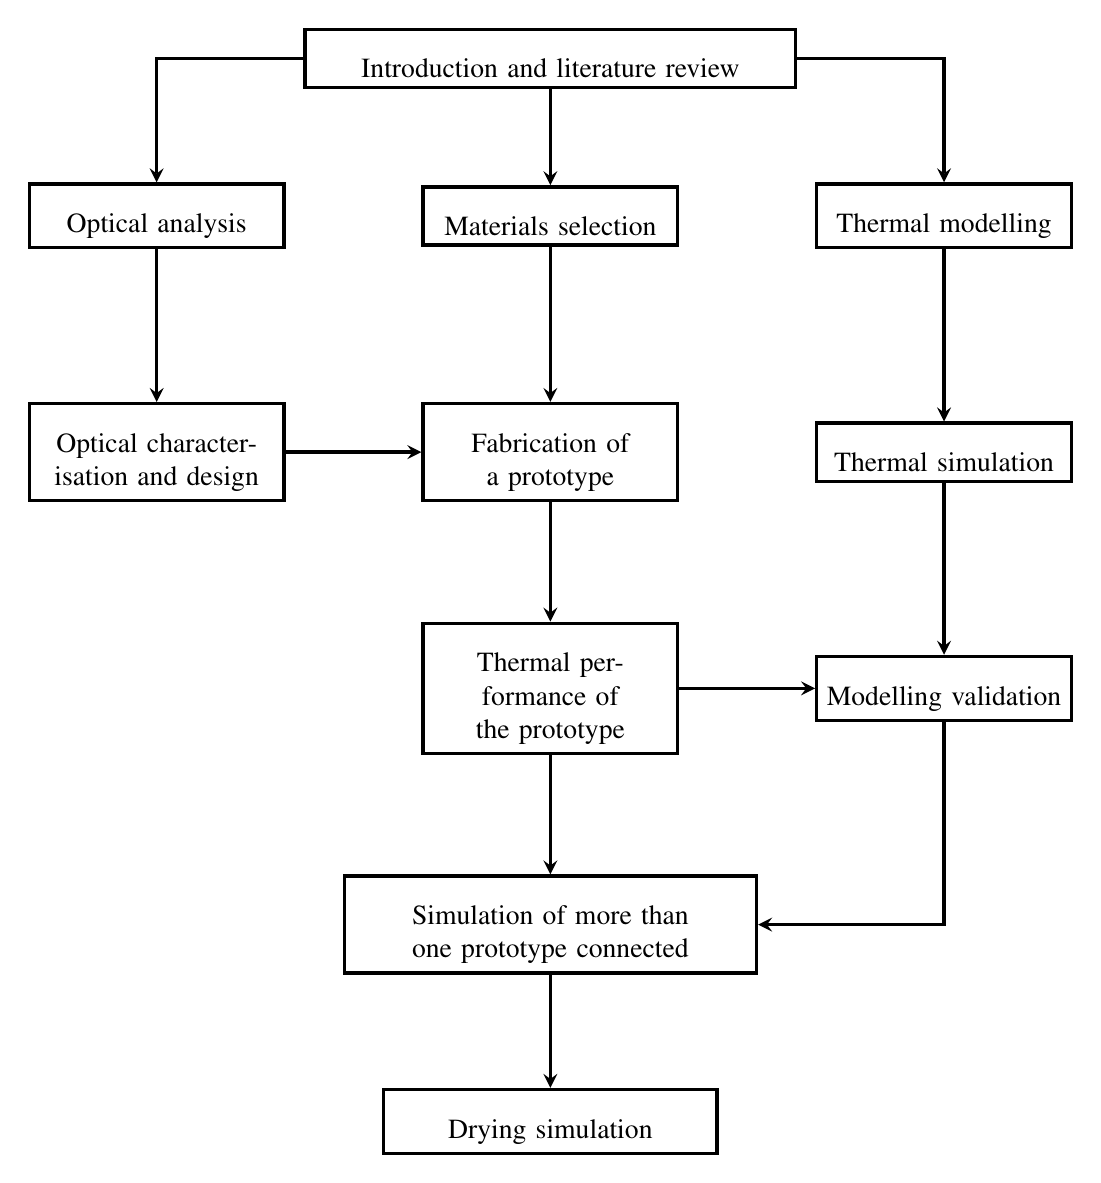
\begin{tikzpicture}[scale=1, node distance = 5 cm, very thick]
		\node[block, text width=6cm] (intro) {Introduction and literature review};
		\node[block, below of=intro,text width=3cm,yshift=3cm] (mat) {Materials selection};
		\node[block, below of=mat,text width=3cm,yshift=2cm] (fab) {Fabrication of a prototype};
		\node[block, below of=fab,text width=3cm,yshift=2cm] (exp) {Thermal performance of the prototype};
		\node[block, left of=mat,text width=3cm] (opt) {Optical analysis};
		\node[block, left of=fab,text width=3cm] (opt2) {Optical characterisation and design};
		\node[block, right of=mat,text width=3cm] (thermal) {Thermal modelling};
		\node[block, right of=fab,text width=3cm] (thermal2) {Thermal simulation};
		\node[block, right of=exp,text width=3cm] (vali) {Modelling validation};
		\node[block, below of=exp,text width=5cm,yshift=2cm] (two) {Simulation of more than one prototype connected};
		\node[block, below of=two,text width=4cm,yshift=2.5cm] (dry) {Drying simulation};
		\draw[arrow] (intro) -- (mat);
		\draw[arrow] (mat) -- (fab);
		\draw[arrow] (fab) -- (exp);
		\draw[arrow] (exp) -- (two);
		\draw[arrow] (intro) -| (opt);
		\draw[arrow] (opt) -- (opt2);
		\draw[arrow] (opt2) -- (fab);
		\draw[arrow] (intro) -| (thermal);
		\draw[arrow] (thermal) -- (thermal2);
		\draw[arrow] (thermal2) -- (vali);
		\draw[arrow] (exp) -- (vali);
		\draw[arrow] (vali) |- (two);
		\draw[arrow] (two) -- (dry);
	\end{tikzpicture}
	%\label{scheme-intro}
	\caption{Research methodology.}
	\label{scheme-intro}
\end{figure}

\begin{itemize}
	\item Chapter \ref{Cap:Int} introduces the research topic, highlighting the motivation for the study and clearly defining the problem statement. It presents the research aim, outlines the specific objectives, emphasizes the contribution of new knowledge to the research area, and provides an overview of the methodology used to achieve these goals;
	\item Chapter \ref{Cap:Lit} -- Literature review: It comprehensively surveys the state-of-the-art in solar thermal collectors for medium-temperature applications, focusing on the key factors influencing thermal performance. It presents the optical characteristics of compound parabolic concentrators (CPCs) and explores methodologies for conducting optical analyses. Different designs for optical concentrators are assessed to discover other methods for focusing solar radiation onto an inverted absorber. In conclusion, the chapter presents a summary of building-integrated solar thermal collectors, emphasising their possible applications and advantages;
	\item Chapter \ref{Cap:Opt} -- Optical modelling and design analysis: presents the design of the solar air heating concentrator and the development of a model to calculate optical efficiency. It also depicts details of the concentrator's geometric specification. A 3D ray tracing technique implemented in Matlab software was developed to calculate the energy distribution at the absorber surface and the effect of the end plates on the optical performance;
	\item Chapter \ref{Cap:Exp} -- Experimental performance analysis: it describes the physical properties of the materials, fabrication and experimental characterisation of the built collector prototype at different airflow rates. The performance of the system depends on wind speed, solar radiation, inlet air and ambient temperatures;
	\item Chapter \ref{Cap:Thermal} -- Heat transfer modelling and simulation: depicts the heat transfer model developed to characterise and simulate the thermal performance of the proposed solar air heater in operation. This model was used to calculate the outlet airflow temperature and thermal efficiency, and experimental data was used to validate the model. Then, the model was used to simulate the thermal performance of collectors connected in series and parallel. Lastly, the validated model was used as an energy input for simulating barley drying to meet the energy demand for an application;
	\item Chapter \ref{Cap:Con} -- Conclusions: It concisely summarises each chapter and key findings, and offers thoughtful recommendations for future work to build on the study's outcomes.
\end{itemize}



	\chapter{Literature Review}
\label{Cap:Lit}
%

This chapter depicts the concept and characteristics of solar air heating collectors -- unglazed and glazed collectors. Considerations were given to:

\begin{itemize}
	\item Elements and factors to affect collector's performance;
	\item Optical concentrator, specifically ACPC with inverted absorber;
	\item Building integration of solar thermal systems.
\end{itemize}


\section{Solar air heating collectors}

Solar air heating collectors (SAHCs) are equipment designed to receive solar radiation and convert it into heat for working air heating. They are widely applied in many commercial applications, such as hot air supply to shopping malls, agricultural barns, industrial drying, etc. They are usually low-cost, with no freezing and high-pressure problems. Compared to water-heating solar collectors, SAHCs are outperformed due to their air thermal properties (\cite{Buker2015}). To overcome this challenge, the heat transfer from the hot absorber surface of the collector to the air needs to be enhanced while the collector's overall heat losses are minimised. (\cite{Shams2013}).

SAHCs can be classified into two main types: unglazed and glazed. The fundamental difference between these types is the presence of a glazing cover and the shape of the absorber surface. Unglazed air heating collectors (also known as Unglazed Transpired Solar Collectors -- UTSCs) do not have any glazing cover; they are composed of a perforated (transpired) absorber plate, as shown in Figure \ref{unglazed-glazed}(a). The absorber plate can be integrated into building fa{\c c}ades. The contact between the absorber plate and ambient air is increased by drawing air through the multiple perforations into the cavity (also called plenum) between the plate and the fa{\c c}ade (\cite{Shukla2012}). A fan pulls this heated air in the plenum into the building (\cite{Buker2015}).

The other main type is the glazed SAHC (or Glazed Air Heating Collector -- GAHC), which has at least a flat glazing cover to prevent the absorber from being exposed to the ambient and avoid efficiency losses. A typical design can be seen in Figure \ref{unglazed-glazed}(b). The air is pulled into the collector by a fan to be heated after contact with the absorber plate, which can have different shapes and/or other modifications to enhance the transfer mechanism.

\Figure[scale=0.58,placement=!ht,label={unglazed-glazed},caption={Illustration of (a) an unglazed and (b) a glazed solar air heating collector. From \citet{Kutscher1994} and \citet{SolarTribune2011}.}]{figs/unglazed-glazed.png}    

To improve the heat transfer from the hot absorber surface to the working air, a wide range of designs for SAHCs has been studied and reported in the literature: glazed, unglazed, bare plate, back-pass, perforated, un-perforated, single, double or triple passes, etc. (\cite{Kutscher1994}; \cite{Christensen1997}; \cite{Gawlik2005}; \cite{Koyuncu2006}; \cite{Leon2007}; \cite{Tchinda2008}; \cite{El-Sebaii2010}; \cite{Athienitis2011}; \cite{Zheng2016}; \cite{Li2016}). %To understand how SAHCs' thermal efficiency is improved, it is worthy defining the response variables to quantify the performance, depicted as follows: 

\subsection{Energy analysis}

Defining the response variables is worth quantifying to understand how SAHCs' thermal performance is improved. The thermal efficiency is defined as the ratio of useful energy rate collected by the working fluid to the incoming total solar radiation $\rm{I_{\!_T}}$ (W/m$^{2}$) received on the aperture area $\rm{A_{apt}}$ (m$^{2}$), calculated by Eq. (\ref{ThermalEf0}). Such efficiency can be evaluated either instantaneously or as an average over a certain period (\cite{Goswami2015}):

\begin{equation}
	\mathrm{\mathlarger{\eta}_{\mathrm{th}} = \frac{Q_u}{I_{\!_T}A_{apt}}}
	\label{ThermalEf0}
\end{equation}

\noindent where the useful energy rate $\rm{Q_u}$ (W) can be calculated considering the airflow rate $\rm{m_{air}}$ (kg/s), the temperature difference between outlet and inlet (\textdegree C), and the specific heat of the air (J/(kg.\textdegree C)) at constant pressure:

\begin{equation}
	\mathrm{{Q_u} = {m_{air}}{C_{p,air}}({T_{out}} - {T_{in}})}
	\label{usefulenergy0}
\end{equation}

The thermal characterisation of an SAHC relates the thermal efficiency under steady-state conditions to each temperature rise normalised by the corresponding solar radiation according to the Hottel-Whillier-Bliss equation, expressed by Eq. (\ref{hottel-whiller-eq0}).

\begin{equation}
	\mathrm{\eta_{\rm{th}} = \eta_o - {U_{\!_L}}\frac{(T_{abs} - T_{amb})}{I_{\!_T}}}
	\label{hottel-whiller-eq0}
\end{equation}

\noindent where $\rm{U_{\!_L}}$ is the collector's overall heat loss coefficient (W/(m$^2$.\textdegree C)) and both absorber and ambient temperatures ($\rm{T_{abs}}$ and $\rm{T_{amb}}$) are in \textdegree C. The $\rm{U_{\!_L}}$ value depends weakly on temperature, and, in most cases, it is considered constant at typical operating conditions (\cite{Rabl1985}). Lastly, the optical efficiency $\eta_{\rm{o}}$ is the ratio between the absorbed and the incident solar radiation. From this equation, $\eta_{\rm{th}}$ can be plotted against $\rm{(T_{abs} - T_{amb})/I_{\!_T}}$, resulting in a linear curve, with $\eta_{\rm{o}}$ and $\rm{{U_{\!_L}}}$ as the linear coefficient and the slope, respectively (\cite{Goswami2015}). 

Another way to calculate the efficiency is based on the air temperature, particularly $\rm{T_{in}}$ and $\rm{T_{out}}$ at the inlet and outlet of the collector, respectively (\cite{Duffie2013}). Eq. (\ref{hottel-whiller-eq0}) can be rewritten by adding a multiplicative term known as the heat removal factor or heat exchange effectiveness. It is defined as the ratio of the heat transferred to the airflow to the maximum possible heat transfer if the outlet air temperature was heated to the absorber surface temperature (\cite{Kutscher1994}). In practice, as the air temperature approaches the absorber temperature, the heat transfer rate slows, requiring infinitely large surface areas or time to achieve the maximum possible heat transfer. This effectiveness is calculated as follows:

\begin{equation}
	\mathrm{\varepsilon_{\!_{HX}} = {\frac{{{T_{out}} - {T_{in}}}}{{{T_{abs}} - {T_{in}}}}}}
	\label{heat-exchange}
\end{equation}

This effectiveness can also be written as a function of the airflow rate and the convective heat transfer coefficient ($\rm{h_{\!_{HX}}}$):

\begin{equation}
	\mathrm{\varepsilon_{\!_{HX}} = 1 - exp\left(-\frac{h_{\!_{HX}}A_{abs}}{m_{air}C_{p,air}}\right)}
	\label{effectiveness}
\end{equation}

\noindent where this convective coefficient $\rm{h_{\!_{HX}}}$ (W/(m$^2$.\textdegree C)) considers the heat transfer mechanism between the airflow and the hot absorber plate. It is related to the Nusselt number, which is the ratio of convective to conductive heat transfer (\cite{Incropera2006}). This is calculated by Eq. (\ref{Nusselt}):
	
\begin{equation}
	\mathrm{Nu = \frac{L_c}{k_{air}}{h_{\!_{HX}}}}
	\label{Nusselt}
\end{equation}

\noindent where $\rm{L_c}$ is the characteristic length of the heat transfer (m) and $\rm{k_{air}}$ is the air thermal conductivity (W/(m.\textdegree C)). The Nusselt number is usually a function of the Reynolds number, which is proportional to the air velocity. Therefore, operating a solar collector with higher airflow rates is desirable to enhance heat transfer. In addition to that, many other factors influence the heat transfer mechanism. The following section describes the elements of a SAHC and how they influence its thermal performance. These elements are the absorber plate, glazing cover, air flow rate and system modifications.

\subsection{Effect of absorber surface}  

As the airflow to be heated goes through a perforated absorber surface, the heat transfer mechanism between the holes and the air is more effective compared to flat plate collectors. The absorber design considers the following factors: i) material and coatings, ii) shape, iii) thickness of the absorber, and iv) modified area.

\subsubsection{Absorber material and coatings} 

It was previously assumed that a collector's high performance resulted from highly thermally conductive materials. This assumption was based on the fact that a significant portion of the thermal energy was transferred to the airflow. Plus, it would considerably increase the average surface temperature and, consequently, the radiative heat loss to the ambient (\cite{Gawlik2002}; \cite{Gawlik2005}).

\citet{Christensen1997} compared experimentally the thermal performance of an UTSC for two absorber materials: aluminium (k = 216 W/(m.K)) and styrene plastic (k~=~0.16~W/(m .K)), where both surfaces had the same geometry. Results show that the UTSC's efficiency is relatively insensitive to low thermal conductivity materials. This means sufficient thermal energy is from the absorber surface to the air, so high thermal conductivity materials are not as critical as previously assumed.

\citet{Arulanandam1999} simulated a UTSC's thermal performance in CFD under no wind conditions, varying the absorber's thermal conductivity from 0.196 to 15.121~W/(m.K)). They concluded that, for low porosity plates, the heat exchange effectiveness dropped by 10 -- 20\%, but the thermal efficiency only decreased by approximately 5\%.

The temperature distribution along the absorber surface can vary for low-conductive materials. The local convective heat transfer is higher in regions of higher surface temperature and lower in regions of lower surface temperature. This effect is reduced if the hole pitch is small so that a large temperature gradient is not achieved. \citet{Gawlik2005} showed that the effect of material conductivity on thermal performance is negligible. The study then concluded that low thermal conductivity materials can be used with no thermal efficiency penalty but a significant benefit in cost savings and corrosion resistance.

One or both of the front and back surfaces of the absorber may be dark in colour to absorb solar radiation. Surfaces may be treated or coated to have a low emittance of infrared radiation to reduce heat losses. The effect of the radiative properties absorptivity and emissivity has also been reported. \citet{Leon2007} simulated a UTSC varying the values of both properties and found that absorptivity substantially affects thermal efficiency more than emissivity. \citet{El-Sebaii2010} simulated a single-pass GAHC comparing absorber surfaces using different coatings. They concluded that the highest daily efficiency was achieved using nickel–tin (absorptivity and emissivity of 0.98 and 0.14). Compared to a black-painted galvanized iron absorber (0.88 of absorptivity and emissivity), the nickel-tin coated absorber outperformed by 29.23\%. \citet{Li2016} simulated a glazed TSC and found that painting the absorber plate with a selective coating of higher absorptivity and lower emissivity would enhance the heat transfer mechanism from the absorber plate to the plenum and reduce the radiative losses from the absorber surface to the glazing cover. The effect of coating absorptivity on thermal efficiency is more considerable than emissivity's.

\subsubsection{Effect of porosity, perforation diameter and pitch} 

The plate porosity for flat plates is defined as the ratio of perforation area to the total surface area. It can only be calculated by setting values of perforation diameter and pitch. Smaller perforation diameters strengthen the jet impingement and thus increase the heat transfer mechanism (\citet{Li2016}). The pitch (or perforation spacing) more substantially influences heat exchange effectiveness than thermal efficiency. With larger pitches, hot spots tend to develop on regions of the absorber surface away from the perforations (\citet{Arulanandam1999}). However, this effect can be avoided if the distance between the holes is small enough.

\citet{Kutscher1994} investigated the effect of increasing perforation diameter (1.6 mm to 3.2 mm) and pitch (13.5 mm to 27 mm) and verified that the heat exchange effectiveness decreased. \citet{Arulanandam1999} discovered that the Nusselt number was increased in a range of plate porosity from 0.5\% to 2\%. \citet{Decker2001} simulated an UTSC and found that the heat exchange effectiveness decreased with increasing pitch (7 mm to 24 mm) and perforation diameter (0.8 mm to 3.6 mm). They also concluded that 28\% of the air temperature rise occurs in holes of the perforated plate. \citet{Gawlik2005} tested two plates of different porosities (0.3\% and 5\%) and concluded that there was no significant difference in air temperature rise because the perforation diameter was increased and the pitch was decreased by the same proportion. 

According to \citet{Leon2007}, simulation results showed that the airflow temperature rise and heat exchange effectiveness increased with decreasing pitch and perforation diameter. For a constant solar radiation and airflow rate, changing the pitch from 12 to 24 mm with a corresponding change in perforation diameter from 0.8 mm to 1.55 mm resulted in a drop of 5.5 $^{\rm o}$C in the airflow temperature rise. Furthermore, when the porosity was increased, the effectiveness and the thermal efficiency decreased.

\subsubsection{Effect of absorber thickness}   

The effect of the absorber thickness on thermal effectiveness is insignificant when it is smaller than 1.5 mm (\cite{Kutscher1994}). However, for thick absorbers (between 1.6 and 3.6 mm), the heat transfer varies between different perforation areas, thus affecting the collector's thermal performance. \citet{Zomorodian2012} tested UTSCs with two different absorber plate thicknesses and concluded that the thicker was more efficient.

\subsubsection{Effect of the absorber-modified area}

One way to enhance the heat transfer from the absorber to the airflow is to introduce obstacles in the air stream to increase the absorber surface area. These obstacles can be fixed either on the internal face of the absorber, on the back plate or as a combination. These obstacles aim to increase the outlet air temperature and efficiency with minimum losses (\cite{Karsli2007}). Modifications of the absorber area include using finned, wavy, or V-corrugated shapes, as seen in Figure \ref{modified}.

\Figure[scale=0.62,placement=!ht,label={modified},caption={Illustration of GAHCs with different absorber areas: (a) wired, (b) wavy, (c) finned, and (d) V-shaped (or V-corrugated). From \citet{Pottler1999}.}]{figs/modified_area.png}

\citet{Karim2004} studied and compared three types of GAHCs: flat plate, finned and V-corrugated to achieve an efficient design suitable for a solar dryer. They found that the V-corrugated collector is the most efficient and the flat plate one the least. Results show that the V-corrugated collector has 7 -- 12\% higher efficiency than flat plate collectors. \citet{Kurtbas2004} also studied different absorber geometries and concluded that all GAHCs outperform the flat plate collector. \citet{Karsli2007} compared the thermal performance of a finned absorber collector to a flat plate one with no fins and concluded that the finned GAHC is more efficient than the flat plate. This is because the fins create turbulent flow, which leads to a higher heat transfer coefficient, lowering the absorber temperature and reducing the thermal heat loss at the same time. \citet{Alta2010} compared a GAHC with a flat absorber surface to one with a finned absorber and concluded that attaching fins on that surface increases the thermal efficiency. \citet{Assari2011} developed a mathematical model based on the effectiveness method for assessing the thermal performance of a GAHC, where water and air flow simultaneously. Three different channels were used to enhance the collector's performance: rectangular fin, triangular fin (V-corruated) and without fin. Simulation results show that channels with rectangular fins performed the best. \citet{ElSebaii2011} compared the thermal performance of a flat plate collector to a V-corrugated collector. The results showed that the double-pass V-corrugated plate collector is 11 -- 14\% more efficient than the double-pass flat plate collector.

\subsection{Effect of glazing cover} 

A glazing cover plays an important role in suppressing convective heat losses from the absorber plate to the ambient and protecting the solar collector against weather conditions. It also needs to have high transmissivity to the solar spectrum and be extensively opaque to long (or infrared) wavelength radiation emitted by the absorber (\cite{Saxena2015a}). In other words, a glazing cover reduces convective and radiative heat losses while transmitting most incoming solar radiation (\cite{Norton2006}).

Glazing materials commonly used are glass, plastic, and fibreglass. The challenge is to find a material with high transmissivity and low thermal conductivity that is affordable and has the required mechanical properties for building integrated systems. Glass is considered a glazing cover because it is transparent in the solar range and absorbs almost all the infrared radiation re-emitted by the absorber plate. This enhances the collector's thermal efficiency by creating a greenhouse effect (\cite{Khoukhi2006}).

More than one glazing cover may be used to minimise the heat losses from the collector (\cite{El-Sebaii2010}; \cite{Yeh2009}). However, the transmissivity decreases due to increased reflections (\cite{Michalopoulos1994}). \citet{Alta2010} conducted an experimental study comparing a single and double-glazed flat plate collector with a finned absorber. The authors stated that the double-glazed collector performed better and showed a higher air temperature difference.

Reflection losses at the glazing surface depend on the refractive index of the cover material and the structural orientation of the glazing. The lowest reflection losses can be achieved if an antireflective coating with a refractive index between the air and the cover material is used. Investigations have shown that the glass transmittance and solar collector efficiency can be increased by 4\% if an antireflection coating is applied instead of standard glass as the cover plate for the solar collector (\cite{Furbo2003}).  

Glass is also very resistant to scratching and high operating temperatures and practically impervious to the damaging effects of ultraviolet exposure. The incident sunlight transmitted through glass depends on the iron content of the glass, which varies between 85\% and 92\% at normal incidence. While low iron content increases the transmittance of glass, low iron glass is more expensive. Glass can be easily broken, but this can be minimized by using tempered glass, which adds a further cost (\cite{Duffie2013}).

Transparent plastics, such as polycarbonates, polyethylene and acrylics have also been used as glazing materials (\cite{Koyuncu2006}). Their main advantages are resistance to breakage and light weight, and are cheaper than glasses. Their main advantages are resistance to breakage, they are lightweight, and they are cheaper than glasses. The main disadvantages of plastics are high transmittance in the longer wavelength, and deterioration over time due to ultraviolet solar radiation (\cite{Goswami2015}; \cite{Duffie2013}). Additionally, plastics are generally limited in the temperatures they can sustain without deteriorating or undergoing dimensional changes. Although glass is expensive, this is the best glazing material considering 20 years of collector life span (\cite{Shams2013}).

\subsection{Effect of airflow rate}  

The flow rate is the most important factor in the thermal performance of a solar collector. The effects of that have been extensively studied. Experimental and simulation results show that more useful heat is collected when the flow rate increases and overall losses are reduced, thus increasing the collector's thermal efficiency. On the other side, the outlet temperature and the heat exchange effectiveness are decreased (\cite{Christensen1997}; \cite{Ammari2003}; \cite{Leon2007}; \cite{El-Sebaii2010}; \cite{Zomorodian2012}; \cite{Li2016}). A typical relationship between air temperature rise, thermal efficiency and flow rate is shown in Figure \ref{airflow_effect}.

\Figure[scale=0.70,placement=!ht,label={airflow_effect},caption={Graphs of air temperature rise and thermal efficiency against mass flow rate at the steady state. From \citet{Tyagi2012}.}]{figs/airflow_effect.png}

\citet{Ammari2003} simulated a single-pass GAHC and found that the thermal efficiency increased until a certain level of volumetric flow rate, and then it increased at a lower rate. A decreasing pattern could be observed for the air temperature as the flow rate was increased. \citet{Leon2007} simulated a UTSC and observed that the decrease in energy rate is lower at lower approach velocities. They also concluded that the collector efficiency decreases with increasing outlet air temperatures. \citet{Jafarkazemi2013} simulated a flat plate collector and also observed that the overall heat loss coefficient dropped as the mass flow rate increased. \citet{Badache2014} and \citet{Nowzari2015} analysed different factors affecting UTSC and GAHC performances and concluded that the airflow rate strongly influenced thermal efficiency. \citet{Li2016} evaluated the performance of a GAHC with a perforated absorber, considering the fan power required to overcome airflow resistance through the collector. In this case, higher airflow rates lead to higher useful heat collected and fan power required. Results show that there is a level of airflow rate that maximises energy efficiency.

\subsection{System modification}

This topic depicts the influence of the airflow passing through the collector in contact with the absorber, the parameterisation of the channel dimension through which the air flows, and how multiple collectors are connected (series or parallel).

\subsubsection{Air passage through the collector}

Considerations are given to the airflow contact with the absorber plate (or PV module) when the former passes through the collector. A single-pass collector is when the airflow comes into contact with the absorber only once. Alternatively, it is double-pass collector when air flows in contact with the absorber twice, as shown in Figure \ref{double_pass}. 

\Figure[scale=0.85,placement=!ht,label={double_pass},caption={Illustration of (a) single pass and (b) double pass air heating collector. From \citet{Hegazy2000}.}]{figs/double_pass.png}

\citet{Hegazy2000} simulated a photovoltaic/thermal (PV/T) glazed collector using different modes: air flowing over or below the absorber and even on both sides in a single or in a double pass. The author found out that flowing air on both sides leads to the best performance, considering both applications. \citet{Yousef2008} tested single and double-pass GAHCs and concluded that double-pass achieved higher thermal efficiency and outlet air temperature. \citet{Nowzari2015} investigated a single and double-pass GAHC and concluded that higher efficiencies are achieved using the double-pass mode. \citet{Karim2004} investigated collectors with different absorber configurations. From the efficiency tests in double-pass operation, it is concluded that the efficiency of all collectors increases in double-pass mode.

The effect of external recycling on the GHAC thermal efficiency has been investigated. If operated with an external recycle, the collector's thermal performance is considerably improved, and the desirable effect overcomes the drawbacks. The performance is enhanced with increasing reflux ratio, especially for operating at a lower air flow rate with higher inlet air temperature (\cite{Yeh2009}).

\subsubsection{Channel's dimensions}

\citet{Hegazy1999} showed a criterion for determining the channel's optimum depth-to-length ratio, which maximises the useful energy from GAHCs to operate at a fixed mass rate of airflow. The author also observed that decreasing the depth or increasing the length improves the thermal performance. \citet{Tonui2007} studied a photovoltaic/thermal glazed collector where forced air was used to extract heat from the back of the PV module through a channel. They evaluated the effect of the channel depth (distance between the PV module and the collector's bottom) and the length on the thermal performance at a constant airflow rate. It was verified that the thermal efficiency and air outlet temperature were reduced with increasing channel depth. They also concluded that the thermal efficiency increased with increasing channel length and approached a constant value as the length increased. The same pattern was verified by \citet{Yousef2008} when they investigated the thermal performance of a single-pass GAHC where forced air was pumped above the absorber plate. They also concluded that air temperature and efficiency decreased with increasing channel depth at a constant airflow rate. \citet{Tonui2008} simulated a photovoltaic/thermal glazed collector using natural convection to alleviate the PV module temperature. They found that there is an optimum channel depth that maximises thermal efficiency.

\subsubsection{Connection of collectors}

Solar collector arrays can be connected in series or parallel, each with different thermal performance outcomes. In a series connection system, the total heat transfer of the collectors is higher since the total airflow passes through all collectors. However, the temperature rise in the collectors reduces the thermal efficiency of each progressive collector, and the power consumption to pump the airflow is also higher (\cite{Hastings2000}). A schematic of multiple units in connection is shown in Figure \ref{series-parallel}. 

\Figure[scale=0.65,placement=!ht,label={series-parallel},caption={Schematics of a system with collectors in series and parallel. From \citet{Fanney1981}.}]{figs/series-parallel.png}

\citet{Oonk1979} developed a formula to predict the performance of N collectors in series by deriving the exit temperature of one collector and using it as the inlet temperature of the next collector. \citet{Fanney1981} also developed an equation to predict the thermal performance of collector arrays, both in series and parallel, based on energy balance.

\section{Concentrating collectors}

When it is required to warm the airflow to higher temperatures with high thermal performance, concentrators can be employed to meet the objective. The working principle is to receive solar radiation through a larger area and direct that, using reflectors, to a smaller absorber area. There are different types of concentrating collectors, depicted as follows (\cite{Evangelisti2019}): 

\begin{itemize}
	\item Parabolic trough collector (PTC): consists of a parabolic reflector and an absorber placed along the whole length of the concentrator at the parabola's focus. PTCs generally track the Sun using east-west, north-south, or polar orientations. The absorber is usually tubular and enclosed in a glass tube to reduce radiative and convective losses (\cite{Goswami2015}). The solar radiation is reflected torward the tube, bringing it to high temperatures and heating the heat-transfer fluid that flows inside it. The absorber temperature varies between 50 $^{\rm{o}}$C and 300 $^{\rm{o}}$C, but it can also reach \mbox{400 $^{\rm{o}}$C};
	
	\item Compound parabolic concentrator (CPC): A CPC consists of two distinct parabolic segments, with each segment's focus positioned at the opposite end of the absorber surface. The axes of these parabolic segments are tilted away from the CPC's central axis by the acceptance angle $\theta_{{\rm{acc}}}$;
	
	%It is designed from two distinct parabolic segments, where the focus of each one is located at the opposing absorber surface end points. The axes of the parabolic segments are oriented away from the CPC axis by the acceptance angle $\theta_{{\rm{a}}}$. The slope of the reflector surfaces at the aperture is parallel to the optical axis for untruncated CPCs;
	
	\item Heliostat field collector: composed of flat reflectors placed all around a central receiver, called solar tower. These reflectors can face the Figure through a tracking system. Central receivers can achieve temperatures of 1000 $^{\rm{o}}$C or even higher. Therefore, a heliostat collector is suitable for thermal electric power production of 10 -- 1000~MW (\cite{Goswami2015});
	
	\item Linear Fresnel collector: comprised of linear receivers and reflectors. The reflector segments are aligned horizontally, facing the Sun so that the rays can hit the receiver without needing movement;
	
	\item Parabolic dish collector: characterized by a paraboloidal geometry that concentrates solar radiation onto a receiver placed at the focal point of the collector.
	
\end{itemize}

\subsection{Optical analysis}

One way of evaluating a concentrator is by characterising its optical performance. Optical efficiency is defined as the ratio between the absorbed and the incident solar radiation. For this analysis, the optical properties of the reflectors, glazing cover and absorber should be taken into consideration, as well as the reflectors' shape and the concentration ratio (\cite{Sellami2013}):

\begin{equation}
	\mathrm{\eta_o = {\tau_{col}}\tau_{glaz}\alpha_{abs}}
	\label{optical0}
\end{equation}

\noindent where the term $\rm{\tau_{col}}$ considers the number of reflections at the reflectors. The reflector's shape and concentration ratio dictate the number of reflections and, consequently, the optical efficiency. The term $\rm{\tau_{glaz}}$ is the transmissivity of the glazing cover; alternatively, for collectors without cover or glass-tube absorbers, this term is unity. The term $\rm{\alpha_{abs}}$ is the absorptivity of the absorber plate. Therefore, it is desirable that the concentrator transmits most of the solar radiation through the glazed aperture, has a highly reflective reflector surface, and has a high absorptivity absorber with low emissivity. Most of these properties have been discussed in the previous section of this Chapter.

Other factors are taken into consideration: i) incoming solar radiation and its components; ii) the position of the Sun at a specific location and what direction the concentrator is facing at a set inclination; iii) the optics in the glazing cover, and; iv) the effect of truncation. Other factors, such as the parabolic shape of a CPC collector and concentration ratio, will be further investigated in another section.

%The shape of reflectors affects size, angular acceptance range (\cite{Zacharopoulos2000}; \cite{Harmim2012}) and maximum geometric concentration ratio (\cite{Mills1978}). Given the same level of concentration ratio, concentrators of narrow angular acceptance are more efficient so collect higher amounts of the available solar energy (\cite{Sarmah2011}; \cite{Kostic2012}).

%A concentrator is usually truncated. Less reflector material is then required which reduces costs and weight. Figure \ref{untruncated} shows the untruncated and truncated versions of the same concentrator. The effect of truncation on the design parameters concentration ratio, height-aperture width ratio and reflector length has been presented by graphs and equations (\cite{McIntire1979}; \cite{Rabl1976}). Figure \ref{ang_acc} shows the angular acceptance function for an untruncated (full) CPC and for a truncated configuration.
%
%\Figure[scale=0.40,placement=!ht,label={untruncated},caption={Truncated and untruncated CPC with a tubular absorber.}]{figs/untruncated.png}
%
%\Figure[scale=0.60,placement=!ht,label={ang_acc},caption={Angular acceptance function of a full and truncated CPC. Adapted from \citet{Norton1991}.}]{figs/ang_acc2.jpg}
%
%\citet{Carvalho1985} derived analytic expressions of angular acceptance range and evaluated the yearly collectable energy as function of the extent of truncation. Truncated concentrators accept solar rays at broader incident angles, thus collecting more solar energy due to reduction of reflections. \citet{Francesconi2018} simulated a five-CPC assembly's performance in CFD; they concluded that a concentration ratio reduction from 2.0 to 1.96 resulted in a 2\% increase of the system's thermal efficiency.

\subsubsection{Solar radiation and intercept factor}

The total solar radiation ($\rm{I_{\!_{T}}}$) incident on the concentrator's aperture is the sum of the beam ($\rm{I_{\!_{B}}}$) and diffuse ($\rm{I_{\!_{D}}}$) components (W/m$^{2}$). However, since concentrators exploit only part of the diffuse radiation, which is dependent of the collector's concentration ratio CR, the factor $\Gamma$ must be defined as the fraction of total solar radiation accepted. Assuming that the angular distribution of diffuse radiation is isotropic, this factor can be estimated as (\cite{Rabl1980}):

\begin{equation}
	\mathrm{\Gamma  = \frac{\displaystyle {\left( {{I_{\!_B}} + \frac{{{I_{\!_D}}}}{CR}} \right)}}{{{I_{\!_T}}}}}
	\label{xi}
\end{equation} 

\noindent and therefore the incoming solar radiation available to reach the absorber surface is assumed to be $\rm{I_{\!_T}\Gamma}$. Since CPC collectors operate in the concentration ratio range of 2 to 10 to capitalise on the corresponding reduced tracking requirement, diffuse radiation is accepted by one-half to one-tenth of the incident (\cite{Goswami2015}). 

It is important to highlight other angular distributions of the diffuse insolation that can affect the performance of PTC and CPC collectors. Two other particular distributions can be considered: cosine and hybrid Gaussian. The hybrid Gaussian distribution combines an isotropic background with a circumsolar Gaussian part. This distribution is more realistic for a tracking system than the isotropic model (which underestimates the insolation intensities at incidence angles near zero) and the cosine model (which underestimates the intensities at large incidence angles). The analytical expressions for the three distributions considered have been presented by \citet{Prapas1987}. However, on clear days (diffuse radiation is approximately 11\% of total radiation), the difference in optical efficiency between the three distributions of diffuse radiation is insignificant.

\subsubsection{Collector's inclination and orientation}

It is important to establish the position of the collector's aperture considering its inclination concerning the horizontal plane and the Sun's position as a function of the day, time and location. Figure \ref{Figure_orientation} shows a basic scheme of the Sun's position by the altitude ($\rm{a_s}$) and azimuth ($\rm{\gamma_s}$) solar angles, as well as the inclination $\beta$ and the collector azimuth angle $\rm{\gamma_{col}}$. The latter defines the orientation of the collector: if $\rm{\gamma_{col}} = 0$, the collector is south-facing.

\Figure[scale=0.80,placement=!ht,label={Figure_orientation},caption={(a) Altitude solar angle, surface azimuth angle, and solar azimuth angle for an inclined surface. (b) Plan view showing solar azimuth angle. Adapted from \citet{Duffie2013}.}]{figs/Figure_orientation.png}

The incident angle $\theta_{\rm{i}}$, defined as the angle between the incident solar ray and the normal to the aperture, is calculated by Eq. (\ref{incidence0}):

\begin{equation}
	\mathrm{\theta_i = {\cos ^{-1}}\left[ {\cos {a_s}\cos ({\gamma_s} - {\gamma_{col}})\sin \beta  + \sin {a_s}\cos \beta} \right]}
	\label{incidence0}
\end{equation}

Solar hour angles ($\omega_{\rm{s}}$) were obtained from the solar time for each day of operation. The solar altitude and solar azimuth angles were calculated from (\cite{Duffie2013}):

\begin{equation}
	\mathrm{{a_s} = {\sin ^{ - 1}}\left( {\sin \phi \sin {\delta _s} + \cos \phi \cos {\delta _s}\cos {\omega_s}} \right)}
	\label{solar_alt0}
\end{equation}
\vspace*{-0.5cm}
\begin{equation}
	\mathrm{\gamma_s = {\sin^{-1}}\left(\frac{\cos \omega_s \sin \delta_s}{\cos a_s}\right)}
	\label{azimuth0}
\end{equation}

\noindent where the solar declination $\delta_{\rm{s}}$ is a function of the year's day and $\phi$ is the location's latitude.

\citet{Pottler1999} calculated the total energy collected for a GAHC at north, south, west and east orientations located in the Northern Hemisphere and verified that the south-facing orientation collects more energy because it is optically more efficient. \citet{Roux2016} used a ray tracing simulator to calculate a flat plate collector's optimum inclination and azimuth angle at different locations. Results showed that an optimally positioned collector can, on average, collect 10\% more annual solar energy than a horizontally fixed collector. The optimum fixed inclination angle is similar to the location's latitude, and the optimum fixed azimuth angle is a function of the longitude angle minus the absolute latitude angle.

\subsubsection{Glazing optics}

By Snell's law, considering the angle of incidence at the glazing cover ($\theta_{\rm{i}}$), the angle of refraction is calculated by Eq. (\ref{snell}):

\begin{equation}
	\mathrm{\theta_r = arcsin\left(\frac{sin\theta_{i}}{n_{idx}} \right)  }
	\label{snell}
\end{equation}

\noindent where $\rm{n_{idx}}$ is the refraction index of the glazing cover dependent of the material. When passing through the glazing medium, part of the incident radiation is reflected and absorbed. The term that takes into account the reflected radiation alone is given by Eq. (\ref{rho_glaz}):

%\begin{equation}
%	\mathrm{r_{par} = \frac{tan^2(\theta_r - \theta_i) }{tan^2(\theta_r + \theta_i) } }
%	\label{parallel}
%\end{equation}
%
%\begin{equation}
%	\mathrm{r_{perp} = \frac{sin^2(\theta_r - \theta_i) }{sin^2(\theta_r + \theta_i) } }
%	\label{perpend}
%\end{equation}

\begin{equation}
	\mathrm{\rho_{glaz} = \frac{1}{2}\left[\frac{1 - r_{par}}{1 + (2N_c - 1)r_{par}} + \frac{1 - r_{perp}}{1 + (2N_c - 1)r_{perp}}\right]}
	\label{rho_glaz}
\end{equation}

\noindent where $\rm{N_c}$ is the number of glazing covers, and $\rm{r_{par}}$ and $\rm{r_{perp}}$ are the unpolarized components of the radiation, functions of the angles of incidence and refraction (\cite{Duffie2013}). Similarly, the term that considers the glazing absorptivity $\rm{\alpha_{glaz}}$ is given by Eq. (\ref{abs_glaz}):

\begin{equation}
	\mathrm{\alpha_{glaz} = exp\left(-\frac{K_{ext}\delta_{glaz}}{cos\theta_r} \right) }
	\label{abs_glaz}
\end{equation}

\noindent where $\rm{\delta_{glaz}}$ is the glazing thickness and $\rm{K_{ext}}$ is the extinction coefficient which is a function of the material: for glass, the value of this coefficient varies from approximately 4 m$^{-1}$ for ''water white'' glass to nearly 32 m$^{-1}$ for high iron oxide content (greenish cast of edge) glass. Lastly, the glazing transmissivity $\rm{\tau_{glaz}}$ can be approximated by the product of the glazing absorptivity and the standalone transmissivity as a function of the glazing material and the incidence angle:

\begin{equation}
	\mathrm{\tau_{glaz} \cong \rho_{glaz}\alpha_{glaz}}
	\label{transmi}
\end{equation}



\subsubsection{End losses}

If a linear concentrator is long in an east-west orientation compared to its width and height, it can be assumed to behave as a two-dimensional system where end effects are negligible (\cite{Eames1993a}). The optical analysis must include the end losses for concentrators with short axial lengths, as some reflected solar rays might not reach the absorber under certain obtuse solar incident angles. To account for the end losses, the optical efficiency is multiplied by a factor for that purpose, which is a function of the incidence angle and the collector's geometry. This factor was analytically calculated for imaging parabolic troughs (\cite{Rabl1985}) and linear Fresnel concentrators. End losses have a more substantial influence at high-latitude locations, which could cause the absorber to be entirely in shadow on winter days (\cite{Hongn2015}). \citet{Pu2011} estimated the end-effect for the north-south and east-west linear Fresnel collectors, analyzing the angles between incident solar rays and the tacking axes of the reflectors. They concluded that the end losses can be compensated by increasing the length of the mirror field. \citet{Heimsath2014} quantified optical losses of Fresnel collectors and proposed a corrective end loss factor for end loss modelling. They also observed that the optical losses are higher for wider zenith angles and shorter collectors. \citet{Xu2014} presented an optical analysis and compensation method for the end loss effect of parabolic trough solar collectors with a horizontal north-south axis. The calculation formulae for optical end loss ratio and increased optical efficiency are derived, and various factors affecting them are analyzed. The compensation method is found to be applicable for regions with latitudes over 25$^{\rm{o}}$ and short trough collectors.

\subsubsection{Truncation}

Compared to a simple parabola, a CPC is very deep, and therein lies its main disadvantage: it requires a relatively large reflector area for a given aperture area. For example, for a concentration ratio of 10, the ratio of reflector area to aperture area is approximately 11, while a PTC has a ratio of around 1.2. To overcome this drawback, a large portion of the top of a CPC can be cut off with almost no loss in performance. A CPC will almost always be truncated in practical applications for economic reasons (\cite{Rabl1976}). \citet{Carvalho1985} derived analytic expressions of the angular acceptance range and evaluated the yearly collectable energy as a function of the extent of truncation. Truncated concentrators accept solar rays at broader incident angles, thus collecting more solar energy due to reduced reflections. \citet{Francesconi2018} simulated a five-CPC assembly's performance in CFD; they concluded that a concentration ratio reduction from 2.0 to 1.96 resulted in a 2\% increase in the system's thermal efficiency.

\subsection{The Compound Parabolic Concentrator (CPC) family}

This section depicts the geometry of a symmetric CPC and an asymmetric CPC, as well as a modification to include an inverted absorber.

\subsubsection{Symmetric CPC} 

The compound parabolic concentrator (CPC) is a non-imaging solar concentrator that has the advantages (compared to focusing ones) of i) no need for solar tracking and ii) the ability to collect a portion of diffuse radiation (\cite{Winston1974}). The CPC has been used for heating and PV electricity production (\cite{Jaaz2017}). A typical CPC cross-section is shown in Figure \ref{CPC1}. Solar radiation accepted within the angular acceptance range is focused onto an absorber by reflection at the two symmetrical parabolic reflectors. 

\Figure[scale=0.60,placement=!ht,label={CPC1},caption={Basic CPC with flat plate absorber: (a) cross-section design in 2D and (b) in 3D. From \citet{Duffie2013} and \citet{Winston1974}.}]{figs/CPC-2D-3D.png}

One of the geometric parameters of a CPC is the geometrical concentration ratio, which is the ratio of the aperture to the absorber areas. This parameter has an upper limit calculated by Eq. (\ref{CR}):

\begin{equation}
	\mathrm{CR = \frac{1}{sin\theta_{acc}}}
	\label{CR}
\end{equation}

\noindent where the half-acceptance angle $\rm{\theta_{acc}}$ is the angular limit over which radiation is fully accepted without moving all or part of the concentrator (\cite{Rabl1976a}). If the reflectors are specular, all the solar rays incident at angles within the acceptance range (between $\pm \theta_{\rm{acc}}$) reach the absorber surface. Figure \ref{untruncated} shows the untruncated and truncated versions of the same CPC. The effect of truncation on the design parameters concentration ratio, height-aperture width ratio and reflector length has been presented by graphs and equations (\cite{McIntire1979}; \cite{Rabl1976}). Figure \ref{ang_acc} shows the angular acceptance function for an untruncated (full) CPC and a truncated configuration.

\Figure[scale=0.40,placement=!ht,label={untruncated},caption={Truncated and untruncated CPC with tubular absorber. From \citet{Norton1991}}]{figs/untruncated.png}

\Figure[scale=0.60,placement=!ht,label={ang_acc},caption={Angular acceptance function of a full and truncated CPC. Adapted from \citet{Norton1991}.}]{figs/ang_acc2.jpg}

The shape of reflectors affects the size, angular acceptance range (\cite{Zacharopoulos2000}; \cite{Harmim2012}) and the maximum geometric concentration ratio (\cite{Mills1978}). Given the same level of concentration ratio, concentrators of narrow angular acceptance are more efficient, so they collect higher amounts of the available solar energy (\cite{Sarmah2011}; \cite{Kostic2012}).

The CPC has been extensively studied and reported in the literature. A common case of study considered a CPC where a working fluid passes within the absorber to capture the heat. However, the cavity between the absorber and the glazing cover is filled with dead air, and therefore, convective losses occur due to the temperature gradient. This affects the motion of air, known as natural or free convection. Hence, this free convective heat transfer coefficient $\rm{h_f}$ (W/m$^2$) is calculated as:

\begin{equation}
	\mathrm{h_f = \frac{{{k_{air}}}}{{{L_c}}}Nu_{f} = a{(Ra)^b}}
	\label{hn}
\end{equation}

\noindent where $\rm{Nu_f}$ is the Nusselt number for free convection, the parameters a and b depend on the geometry and the flow regime (\cite{Cengel2005}) and the Rayleigh number is defined as the strength of the thermal buoyancy against the viscous and thermal diffusion.

%The Rayleigh number is defined as the product of the Grashoff and the Prandtl numbers, shown by Eq. (\ref{Ra}):
%
%\begin{equation}
%	\mathrm{Ra = Gr \Pr = {\frac{{g{\beta_{th}}}}{{\nu_{air}^2}}{L^{3}_c}\Delta T^{*}\Pr}}
%	\label{Ra}
%\end{equation}
%
%\noindent where: $\rm{L_{c}}$ is the characteristic length; the volume expansion coefficient $\beta_{\rm{th}}$ is 1/$\rm{T_{air}}$ as the air is considered an ideal gas; $\rm{\Delta T^{*}}$ is the temperature difference between the surface and the air; and $\nu_{\rm{air}}$ is the air kinematic viscosity.

\citet{AbdelKhalik1978} evaluated the natural convective coefficients between the absorber surface and cover plate for vertically oriented two-dimensional CPC using finite-element techniques. The critical Rayleigh number values for different concentration ratios (2 $<$ CR $<$ 10) with three levels of truncated CPCs are determined. Results show that convection is suppressed in high-concentration cavities with a large height/aperture ratio.

%Mathematical formulations were developed to study thermal processes in a compound-parabolic- concentrator (CPC) collector. The system under investigation consists of a CPC cusp fitted with a concentric, evacuated double pipe to serve as a heat absorber. Heat is transmitted to the circulating fluid flowing inside a U-tube via the heat getter slipped inside the inner pipe (\cite{Hsieh1981}).

\citet{Prapas1987} developed a heat transfer model and found out that the Nusselt number is affected by the concentration ratio of the collector, its inclination and the absorber temperature. The average Nusselt number rises as the inclination of the collector increases, and this effect is enhanced for higher concentration ratios. Moreover, generalised correlations for the variation of the Nusselt number have been obtained.

\citet{Eames1993} performed a detailed parametric heat transfer analysis in untruncated CPCs using a model for their optical and thermal behaviour. The effects of inclination and acceptance angles on free convection within the cavity were studied. A convective heat transfer correlation is obtained for the average Nusselt number concerning the Grashof number that considers acceptance angle and angular inclination. They also observed that CPCs of higher acceptance angles have lower Nusselt numbers.

A theoretical and experimental investigation into the modifications in optical and thermal performance resulting from introducing a baffle into the cavity of a CPC has been performed. Results show that introducing a baffle reduces internal convection, reducing heat losses with a slight reduction in optical efficiency (\cite{Eames1995}).

Heat transfer modelling in CPCs has been investigated. This considered the effect of the inclination angle of an east-west aligned collector. The internal and external convective heat transfer correlations employed are angular dependent. The model also considered the contribution of beam and diffuse radiation. The results demonstrate a 10\% variation in convective heat transfer with an angle of inclination for low-concentration CPCs (i.e. CR = 1.5). Furthermore, the thermal efficiency was lower for incoming radiation of more diffuse components. In this case, because of the high diffuse radiation, a CPC of lower concentration would be preferred to maximise the fraction of the diffuse insolation collected. (\cite{Kothdiwala1995}).

The results show that when radiation is neglected, the onset of fluid motion is delayed by the cavity's concentration level. When radiation is considered, it has an important effect on the temperature distribution inside the parabolic cavities and the local and average values of the convective and radiative Nusselt numbers. The emissivity substantially affects the average radiative Nusselt number, especially at high Rayleigh numbers (\cite{Diaz2008}).

\citet{Tchinda2008} developed a mathematical model for computing the thermal performance of a SAHC with truncated CPC having a flat one-sided absorber. The effects of the air mass flow rate, the wind speed and the collector length on the thermal performance of the present collector were investigated. Predictions for the performance of the SAHC also exhibit reasonable agreement, with experimental data with an average error of 7\%.

\subsubsection{Asymmetric CPC}

Symmetric CPCs have two equal half-acceptance angles concerning the optical axis. The asymmetric compound parabolic concentrator (ACPC) introduced by \citet{Rabl1976} is a particular case of its symmetric counterpart. Figure \ref{ACPC} shows a general cross-section of an ACPC, where the acceptance angle is $\rm{2\theta_{acc} = \theta_{\!_{PU}} + \theta_{\!_{PL}}}$. The geometric concentration ratio is also the ratio of the aperture to absorber areas. The axis of the upper (lower) parabola subtends an angle $\rm{\theta_{\!_{PU}} (\theta_{\!_{PL}})}$ perpendicular to the absorber surface. Therefore, broader angular acceptance range and designs with higher concentration ratios can be achieved due to the asymmetry (\cite{Tian2018}). 

\Figure[scale=0.60,placement=!ht,label={ACPC},caption={General design of an asymmetric CPC.}]{figs/ACPC.png}

Asymmetric concentrator systems present the following advantages (\cite{Mills1978}):

\begin{itemize}
	\item Ability to compensate lower solar radiations in the early morning and late afternoon, allowing more uniform output;
	\item Greater operational flexibility for unexpected variations in energy demand and higher yearly average energy input per reflector surface area.
\end{itemize}

Researchers have studied this type of concentrator in detail. \citet{Zacharopoulos2000} analysed the optical performance of a 3D dielectric ACPC with a 78\% truncation at the vertical compared to a symmetric version (Figure \ref{ACPCzac}). The analysis showed that the asymmetric concentrator design is more suitable for use in a building fa\c{c}ade than a symmetric one. Using a dielectric concentrator, an ACPC can collect 40\% of solar radiation with, due to refraction, collection even outside the angular acceptance range. \citet{Tripanagnostopoulos2000} proposed a collector design based on a truncated asymmetric CPC reflector consisting of a parabolic and a circular part. This design features a flat bifacial absorber installed at the upper part of the collector, parallel to the glazing, to form a thermal trap space between the reverse absorber surface and the circular part of the mirror. The experimental results showed that the proposed collector could achieve a maximum efficiency of 71\% and a stagnation temperature of 180 $^{\rm{o}}$C. \citet{Mallick2006} presented a comparative experimental characterisation of a non-imaging line-axis 0~--~50$^{\rm{o}}$ acceptance-half angles asymmetric compound parabolic photovoltaic concentrator (ACPPVC-50) suitable for vertical building fa\c{c}ade integration with its non-concentrating counterpart. \citet{Mallick2007b} performed an optical and heat transfer analysis for a truncated ACPC of concentration ratio 2.01 suitable for photovoltaic applications to use airflow to alleviate temperature at the solar cells. \citet{Sarmah2011} compared the optical performance of three dielectric ACPC designs (all truncated with a concentration ratio of 2.82) of acceptance angles 0 -- 55$^{\rm{o}}$, 0 -- 66$^{\rm{o}}$, and 0 -- 77$^{\rm{o}}$ to optimize the concentrator for building facade photovoltaic applications in northern latitudes ($>$ 55 $^{\rm{o}}$N). Based on the annual solar energy collection by all the designs, it was found that the system of acceptance angles 0 -- 55$^{\rm{o}}$ is more optically efficient and can collect more energy compared to the other two. \citet{Harmim2012} constructed and evaluated the performance of a box-type solar cooker equipped with an ACPC of concentration ratio 2.12. The reflectors were designed so that the absorber could receive solar rays at a solar altitude angle between 30 and 75$^{\rm{o}}$.

\Figure[scale=0.60,placement=!ht,label={ACPCzac},caption={Dielectric ACPC with 78\% truncated at the vertical for building integration photovoltaic.}]{figs/ACPCzac.PNG}

%\Figure[scale=0.70,placement=!ht,label={cooker},caption={Sketch of the box-type solar cooker employing an ACPC.}]{figs/cooker.PNG}

\subsubsection{ACPC with Inverted Absorber}

Collectors employing inverted absorbers, in which solar radiation is reflected from below onto the downward-facing absorbing surface, have been proposed by \citet{Rabl1976} and shown in Figure \ref{col_rev}. They are also called inverted absorber asymmetric compound parabolic concentrators (IACPC). Although optically less efficient due to the multiple reflections of incident solar energy (\cite{Eames1996}; \cite{Kothdiwala1996}; \cite{Shams2013}), this type of concentrator can achieve higher absorber temperatures by suppressing convective and radiative heat losses (\cite{Kothdiwala1997}; \cite{Kothdiwala1999}). This is due to the formation of thermally stratified air layers below the absorber and also because this surface does not view the aperture directly (\cite{Kienzlen1988}; \cite{Eames2001}).

\Figure[scale=0.50,placement=!ht,label={col_rev},caption={Basic CPC geometry with inverted absorber.}]{figs/col_rev.eps}

%Researchers have reported studies aiming to evaluate the performance of this type of collector. 
\citet{Kothdiwala1996} developed a ray trace model to simulate and optimise the IACPC optical performance. This model considered the effect of beam and diffuse radiation separately. They verified that the beam optical efficiency decreases with the cavity height and concentration ratio increase. It was also found that the diffuse optical efficiency is improved when the acceptance angle is increased.

%\Figure[scale=0.70,placement=!ht,label={koth96},caption={Geometry of the CPC with inverted absorber analysed.}]{figs/koth96}

\citet{Eames1996} predicted the thermo-physical performance of the IACPC system. In their study, the energy flux at the absorber was determined by a ray trace technique and a finite element model was developed to predict the system's thermo-fluid behaviour. They concluded that a net gain in efficiency is achieved by including a cavity above the circular reflector due to the convection suppression.
\citet{Kothdiwala1997} conducted indoor experiments under a solar simulator to analyse the performance of the IACPC, which was copper sheeting onto a tubing along the concentrator's long axis. The tests were carried out using water as the flowing fluid at various cavity heights. They found that the overall performance is more efficient for higher gap height configurations.
\citet{Kothdiwala1999} compared a tubular absorber CPC with a glass envelope to an IACPC at different cavity heights for water heating purposes. They concluded that using an absorber configuration on the IACPC maximises convection suppression and minimises optical losses. Furthermore, this system outperforms the others in terms of optimum configuration compared to this study.
\citet{Eames2001} simulated the performance of an IACPC by using a combined ray trace and finite element computational fluid dynamics model previously developed by \citet{Eames1993a}. This model was validated by direct comparison with experimental results.

\citet{Tiwari1998} modelled and evaluated the performance of an inverted absorber solar still for distillation purposes. They found that this inverted configuration provided double the hourly yield compared to a conventional still. The experimental comparison between inverted absorber solar still and conventional single slope solar at various water depths has been conducted by \citet{Dev2011}. They found that the water temperature in an inverted absorber solar basin is still higher than the conventional one.

In order to suppress convection losses, \citet{Smyth2005} investigated the use of transparent baffles at different locations within the collector cavity; the system consisted of an integrated collector storage solar water heater (ICSSWH) mounted in the cavity of an IACPC. \citet{Shams2016} designed and fabricated a concentrating transpired air heating system comprised of an IACPC with a perforated absorber. This collector had the transpired absorber surface made of woven carbon fibre placed at a fixed cavity height, a glazed aperture, a concentration ratio of 2.0, and was experimentally tested at different air flow rates.

\subsection{Optical systems and Ray tracing technique}

A significant part of the design and analysis of concentrating collectors involves ray tracing techniques, which are algorithms to simulate light rays passing through an optical system. Ray tracing analysis is an important method adopted in optical systems to obtain the optical performance for complex geometries regarding direct and diffuse solar radiation (\cite{Ali2013}). Most of its energy will be reflected when a ray hits a reflecting surface. To model this behaviour in a suitable ray tracing procedure, the law of reflection is expressed in vector form (\cite{Winston2005}). Figure \ref{ref_point} shows the unit vectors $\rm{r_{inc}}$ and $\rm{r_{ref}}$ along the incident and reflected rays and a unit vector $\rm{r_n}$ at the normal point of incidence into the reflecting surface. The law of reflection is expressed by Eq. (\ref{ref_law}):

\begin{equation}
	\mathrm{{r_{ref}} = {r_{inc}} - 2({r_n} \cdot {r_{inc}}){r_n}}
	\label{ref_law}
	\end{equation}

\Figure[scale=0.80,placement=!ht,label={ref_point},caption={Law of reflection applied on a reflecting surface.}]{figs/ref_point.eps}

The ray tracing analysis with optical study can provide:

\begin{itemize}
	\itemsep-5pt
		\item The average number of reflections before the incoming rays reach the absorber plate (\cite{Shams2013}; \cite{Benrejeb2016});
		\item Optical efficiency as a function of the incidence angle (\cite{Kothdiwala1996}; \cite{Souliotis2011});
		\item Visualisation of rays' path and reflection points (\cite{Mallick2007}; \cite{Ratismith2014}; \cite{Ustaoglu2016});
		\item The intensity of energy distributed at the absorber surface (\cite{Smyth1999}; \cite{Sellami2013}; \cite{Ali2014}; \cite{Bellos2016});
		\item System's optical characterisation for thermal modelling and simulation (\cite{Mallick2007}; \cite{Shams2013}; \cite{Bellos2016});
		\item Comparison between two or more systems (\cite{Zacharopoulos2000}; \cite{Sarmah2011}; \cite{Wu2009}).
	\end{itemize}

Several concentrating systems have been proposed and optically analysed for different purposes and reported in the literature in detail. \citet{Souliotis2011} used a two-dimensional ray tracing method to analyse the optical properties of an asymmetric CPC collector. The process involved tracing the paths of many rays through the system and calculating the acceptance angle. The results showed that the collector achieves optical efficiencies above 75\% within its acceptance angle, decreasing efficiency rapidly outside this range.

\citet{Sarmah2011} presented the design and optical performance evaluation of stationary dielectric asymmetric compound parabolic concentrators using ray tracing methods. The designed concentrators have a geometric concentration ratio of 2.82 and a maximum optical efficiency of 83\%. The ray tracing simulations show that all rays within the acceptance half-angle range can be collected without escaping from the concentrator's aperture.

\citet{Zheng2011} presented a new multiple chamber trough solar collector, and optical analysis software was used to simulate the ray tracing of the solar light concentrating system. The study investigated the flat and cylindrical receivers and the relationship between the receiving beam and the incident ray. The simulation results showed the image's distribution, width, eccentric magnitude, and efficiency of the concentrated light varying with the incident angle. The concentration ability of the system with a flat receiver and a cylindrical receiver was quantitatively analysed and compared.

Using the OpticsWorks software, \citet{Sellami2012} performed an optical analysis. They developed a novel geometry of a 3D static concentrator as a square elliptical hyperboloid (SEH) to be integrated into glazing windows or fa\c{c}ades for photovoltaic applications. The SEH of concentration ratio 4.0 was optically optimised considering different incident angles of the incoming light rays.

\citet{Ali2013} evaluated the optical performance of a static 3D elliptical hyperboloid concentrator using a ray tracing software called Optis. Effective concentration ratio, optical efficiency and geometric parameters were analysed. Furthermore, the geometry was optimised to improve the overall performance.

\citet{Binotti2013} proposed an analytical approach to evaluate the impact of 3D effects on the optical performance of parabolic trough collectors. The approach extends the First-principle OPTical Intercept Calculation (FirstOPTIC) method and was validated against numerical solutions and ray-tracing simulation results. The new approach was applied to case studies to examine the impact of 3D effects on the intercept factor, and a correction was proposed for the approach generally accepted for specularity mirror errors for non-zero incidence angles.

\citet{Sellami2013} developed a 3D ray trace code in Matlab to determine the beam optical efficiency and the energy distribution of a 3D crossed CPC (CCPC) for different incident angles. The authors found that this type of CPC is an ideal concentrator for a half-acceptance angle of 30$^{\rm{o}}$ and a concentration ratio of 3.6.

\citet{Ali2014} presented the design and experimental analysis of a 3D solar elliptical hyperboloid concentrator (EHC) for process heat applications. Ray tracing analysis was used to obtain the solar flux distribution on the receiver aperture plane, and the optical efficiency was obtained theoretically using a ray tracing program. The design was optimized before finalizing and experimentally testing the EHC.

\citet{Abu-Bakar2014} proposed a new type of concentrator, the rotationally ACPC, for use in building integrated systems for PV applications, where the geometrical and optical concentration gain were evaluated. From the simulations, it has been found that the concentration could produce an optical concentration gain as high as 6.18 when compared with the non-concentrating cell, depending on the half-acceptance angle.

\citet{Ratismith2014} proposed non-tracking configurations of solar collector modules designed to operate efficiently during the day for varying incident angles of direct and diffuse radiation. The design criteria for achieving a high intercept factor without tracking throughout the day are emphasised by conducting ray tracing analysis on different trough shapes and absorber plate orientations. Furthermore, the superiority of the flat base-collector over the double-parabolic design was demonstrated.

\citet{Abdullahi2015} investigated the optical efficiency of two tubular receivers in a compound parabolic concentrator or a single elliptical receiver. Ray tracing is used to predict the optical efficiency, and the results show that the horizontal configuration outperforms the single and vertical configurations by up to 15\%. Moreover, the horizontally aligned elliptical single-tube configuration increases the average daily optical efficiency by 17\% compared to the single-tube configuration.

\citet{Benrejeb2015} used mathematical equations describing the geometric design of an integrated collector storage system. Therefore, an optical study was given with details on achieving the ray tracing technique results and the energy flux distribution on the absorber surface. Furthermore, the optical results were used as inputs in the heat transfer model to simulate the temperature of the water inside the absorber.

\citet{Benrejeb2016} worked on a numerical model based on a ray tracing technique to study the effect of truncation on the optical and thermal performances of an integrated collector storage system of solar water heaters with asymmetric CPC reflectors. The model can predict both full and truncated CPC systems and the simulation involves analysing several parameters such as geometric concentration and half acceptance angle. The effect of truncation on ray trace diagrams and its impact on optical and thermal performances was also studied.

\citet{Bellos2016} performed an optical analysis and optimised the geometry of a CPC with an evacuated tube, where this design is considered to be optimum because all the reflected rays reach the receiver. They also calculated the optical losses at different solar angles. The authors also indicate the need to track the collector to minimise the incident angle. \citet{Qin2013} designed and optimised the geometry of an aspheric reflecting solar concentrator to focus sunlight on a narrow line segment. They used a particular aspheric equation in three dimensions and the law of reflection to trace the incident rays.

\citet{Ustaoglu2016} developed an optical analysis on a cylindrical CPC to reduce hot spots on a PV cell caused by non-uniform solar irradiation. Different truncation levels were tested to determine the optimum optical and thermal efficiency levels. The study analysed average efficiency, incident angle, and annual performance for different absorber surfaces. Heat flux and temperature distribution on the absorber were also evaluated to determine the uniformity of solar illumination.




\section{Building integration of solar systems}



%In addition to being technically and structurally efficient, solar thermal collectors must satisfy criterion summarised in the IEA Task 41 Solar Energy and Architecture for aesthetic quality of buildings integrated solar thermal collectors [4]:

%\begin{itemize}[topsep=5pt,partopsep=0pt] \itemsep0pt
%	\item Integrating naturally; 
%	\item Architecturally pleasing design;
%	\item Consistency to the context of the building;
	%\item Size that suits the harmony and combination;
%	\item Good composition of colours and materials;
%	\item Well composed and innovative design.
	
%\end{itemize}

A building-integrated solar thermal system (BISTS) is a solar thermal collector integrated into a building to meet local energy requirements. This integration must consider functionality (useful thermal energy, thermal insulation, shading, construction stability) and/or appearance aspects (aesthetics, dimensions, shape, colour of the building). In addition to that, they need to be technically and structurally efficient (\cite{Wall2012}; \cite{Buker2015}). A few more factors will need to be taken into consideration, such as (\cite{COSTOffice2015}): i) amount of useful thermal energy collected and fluid temperature delivered; ii) resistance to weather conditions; iii) light and solar energy characteristics in case of transparent layer; iv) thermal resistance and thermal transmittance characteristics of the construction (overall heat transfer coefficient); v) fire protection, and; vi) noise attenuation.
 
% coupled onto the exterior of a building -- usually mounted on the fa\c{c}ade or on the roof -- to meet local energy requirements.



% These systems' designs must consider architectural aspects, such as colour, materials, texture and shape, enabling a more homogeneous building aesthetic than conventional solar thermal collectors. Plus, they need to integrate harmony with the building, be consistent with the building context, and be of well composed and innovative design. In addition to that, they need to be technically and structurally efficient (\cite{Wall2012}; \cite{Buker2015}).

%Building integrated solar thermal system: We consider STS as building integrated, when some components (mainly the solar thermal collector) is an integral part of the building functionality, not just an added element. This integration may be functional (i.e. thermal insulation, shading, construction stability etc. will be compromised) and/or relates to the appearance (aesthetics, dimensions, shape, colour etc. of the building). Thus building integration considers architectural integration in form and function.

These systems have been classified across operating characteristics, features, and mounting configurations. The main classification criteria of all solar thermal systems are based on the method of transferring collected solar energy to the application (active or passive), the thermal transfer fluid (air, water, water-glycol, oil, etc.) and the final application for the energy collected (hot water and/or space heating, cooling, process heat or mixed applications). In the passive or active classification, in the first case, the thermal transfer fluid flows by natural convection or circulation or no transport at all. In the second case, pumps or fans circulate the fluid to a point of demand or storage (forced convection or circulation). However, several systems are hybrids, operating by natural and forced transport methods. Many fa\c{c}ade solar air heaters use thermal buoyancy to induce airflow through the vertical cavities that can be further augmented with in-line fans (and heating) if necessary.

The BISTS delivers thermal energy to the building, but other forms of energy may also contribute to the building's energy balance. For instance, daylight comes through a transparent window or fac¸ade collector, or PV/T systems will also deliver electrical power, which may be used directly by any auxiliary electrical services. Heated air or water can be stored or delivered directly to the point of use. Although the range of applications for thermal energy is extensive, all of the evaluated studies demonstrate that the energy is used to provide one or a combination of the following cases:

\begin{description}
	\item[Space heating:] Thermal energy produced by a BISTS may reduce the space heating load of a building by adding solar gains directly (by a passive window) or indirectly (by transferring heat from the collector via storage to a heating element) into the building;
	
	\item[Air heating and ventilation:] Thermal heat may also be used to pre-heat the fresh air needed in the building. Air is heated directly or indirectly to provide heating and/or ventilation space. In some cases, an auxiliary heating system is used to enhance the heat input because of comfort reasons;
	
	\item[Water heating:] Hot water demand in the building is the most popular application. In the majority of water heating BISTS, a customised heat exchanger or integrated proprietary solar water is used to transfer collected heat to a (forced) heat transfer fluid circuit and onto an intermediate thermal store and/or directly to a domestic hot water application; 
	
	\item[Cooling and ventilation:] In cooling-dominated climates, buildings may have an excess of thermal energy, and therefore, BISTS can also be a technology to extract heat from a building. Several methods are described for providing a cooling (and/or ventilation) effect to a building: shading vital building elements, desiccant linings, induced ventilation through a stack effect and reverse operation of solar collecting elements for night-time radiation cooling.
\end{description}

%Air-based BISTs are characterised by lower costs and efficiencies than water heating systems. They are generally used for building ventilation and heating. Hydraulic BISTs are generally used for heating and hot water generation. BISTs that adopt phase change materials are generally used when a longer period of the system output is required. These systems can be categorised in function of the integration with the building envelope, as shown in Figure 9. For many decades integrated solar thermal systems have been studied with research efforts focused on different technological solutions to BIST integration.
%
%Air-based BISTs are solar thermal air collectors integrated on roofs and facades, as shown in Figure 10. These collectors are characterised by low costs but also by a low efficiency due to the thermal characteristics of the air as a heat transfer fluid. Air has low thermal properties, thus influencing convective heat transfer phenomena. To compensate these limits, large collector areas and ducts are needed. However, these can introduce problems related to costs and roof/facade size [23]. Solar thermal facades that use air can be made by integrating an air gap between the rear surface of the glass covers and the building envelope. In space heating systems, constant air flows are generally provided, thus the outlet air temperature varies during the day in function of the solar radiation variations.
%
%Using water instead of air is effective because of its high thermal capacity and thermal conductivity. Water allows easy storage as it is suitable for direct domestic hot water generation, but it is corrosive. %The water-based BIST can be classified into two groups: single-channel and multiple-channel BISTs. The first group has evolved from the passive solar heating mechanism, which often provides solutions for the use of hot water. The second group is characterised by a design with an additional air space between the photovoltaic module and the building envelope.
%
%Roof integrated mini-parabolic solar collector have been studied for building-integrated applications. These systems adopt linear Fresnel reflectors to focus the beam solar radiation on a stationary receiver with the use of mirrors and an active tracking system (ref). The use of concentrating optical system for building integrated solar applications was proposed by Chemisana et al. [25]. The analysis of a stationary wide-angle Fresnel lens with a moving CPC was proposed by the authors. A building integrated mini parabolic thermal collector investigated by Petrakis et al. [26], had a East-West orientation with a slope to receive the Figure's rays perpendicularly during the day. A solar micro-concentrator collector is shown in Fig. 11.
%
%Another solution is represented by the ceramic solar collectors, mainly characterised by economic convenience, without absorption attenuation and good integration in buildings. As asserted by Buker and Riffat [23], the raw material for this system is traditional ceramic (porcelain clay, quartz and feldspar). The building integration of these solar collectors was also proposed by Yang et al. [27]. The collectors act both as heat source of the water system, and as balcony railings, with a thermal efficiency equal to 41.7\%.
%
%Overhang louvre shading modules, placed horizontally, can incorporate solar collectors. This approach allows an increased number of collectors to be installed as space is freed on the building roof for the installation of additional panels. The various designs of solar louvre thermal collector have been discussed by Abu-Zour et al. [28]. They have proposed a design that used heat pipe technology. Marrero et al. [29] analysed a solar thermal system that exploited building louvre shading devices. They proposed the modification of existing designs. The proposed system was tested under several climatic conditions, showing great potential from both an economic and a renewable energy supply point of view.
%
\subsection{Building integrated solar thermal collectors for air heating}

These collectors are known for being cost-effective; however, they also have lower efficiency. This reduced efficiency is mainly due to the thermal properties of air, which is used as the heat transfer medium. The low thermal conductivity of air significantly affects the convective heat transfer within these systems. To overcome these efficiency challenges, it is necessary to implement larger collector areas and duct systems. However, deploying such measures may engender cost escalation and impose spatial constraints on building surfaces. Notably, solar thermal facades employing air as the heat transfer medium can be engineered by incorporating an air gap between the rear surface of glass covers and the building envelope. In space heating applications, consistent air flows are typically maintained, resulting in fluctuations in outlet air temperature throughout the day in response to variations in solar radiation intensity.

%fa\c{c}ade

%Using water instead of air is effective because of its high thermal capacity and thermal conductivity. Water allows easy storage as it is suitable for direct domestic hot water generation, but it is corrosive. The water-based BIST can be classified into two groups: single-channel and multiple-channel BISTs. The first group has evolved from the passive solar heating mechanism, which often provides solutions for the use of hot water. The second group is characterised by a design with an additional air space between the photovoltaic module and the building envelope.

%Roof integrated mini-parabolic solar collector have been studied for building-integrated applications. These systems adopt linear Fresnel reflectors to focus the beam solar radiation on a stationary receiver with the use of mirrors and an active tracking system (ref). The use of concentrating optical system for building integrated solar applications was proposed by Chemisana et al. [25]. The analysis of a stationary wide-angle Fresnel lens with a moving CPC was proposed by the authors. A building integrated mini parabolic thermal collector investigated by Petrakis et al. [26], had a East-West orientation with a slope to receive the Figure's rays perpendicularly during the day. A solar micro-concentrator collector is shown in Fig. 11.

Mini-parabolic solar collectors integrated into roofs have been explored for building integration purposes. These systems utilise linear Fresnel reflectors to concentrate solar radiation onto a fixed receiver by manipulating mirrors and an active tracking mechanism. The study proposed a stationary wide-angle Fresnel lens coupled with a moving CPC. Additionally, a building-integrated mini-parabolic thermal collector was studied in an East-West direction with a slope optimised to intercept sunlight perpendicularly throughout the day.

%Another solution is represented by the ceramic solar collectors, mainly characterised by economic convenience, without absorption attenuation and good integration in buildings. As asserted by Buker and Riffat [23], the raw material for this system is traditional ceramic (porcelain clay, quartz and feldspar). The building integration of these solar collectors was also proposed by Yang et al. [27]. The collectors act both as heat source of the water system, and as balcony railings, with a thermal efficiency equal to 41.7\%.

Ceramic solar collectors offer an alternative solution, notable for their economic viability, minimal absorption attenuation, and seamless integration into building structures. These collectors use conventional ceramic materials such as porcelain clay, quartz, and feldspar. It was also suggested that these solar collectors be integrated into buildings. In this proposed application, the collectors serve dual purposes: providing heat for water systems and serving as balcony railings, achieving a thermal efficiency of 41.7\%. 

%Overhang louvre shading modules, placed horizontally, can incorporate solar collectors. This approach allows an increased number of collectors to be installed as space is freed on the building roof for the installation of additional panels. The various designs of solar louvre thermal collector have been discussed by Abu-Zour et al. [28]. They have proposed a design that used heat pipe technology. Marrero et al. [29] analysed a solar thermal system that exploited building louvre shading devices. They proposed the modification of existing designs. The proposed system was tested under several climatic conditions, showing great potential from both an economic and a renewable energy supply point of view.

Horizontal overhang louvre shading modules offer a space-efficient platform for integrating solar collectors, enabling the installation of more collectors by freeing up roof space for additional panels. It explored various designs of solar louvre thermal collectors, introducing a design incorporating heat pipe technology. Similarly, a solar thermal system utilising building louvre shading devices and suggested modifications to existing designs were investigated. Testing the proposed system under diverse climatic conditions revealed significant potential both economically and in terms of renewable energy supply.

\section{Chapter summary}

This chapter depicted a comprehensive literature review on solar air heating collectors (SAHCs) and related solar thermal technologies, highlighting their design, influencing factors, and diverse applications. SAHCs are widely used for industrial drying, space heating, and agricultural purposes, with two primary types: unglazed collectors, featuring perforated metallic plates without glazing to enhance air contact, and glazed collectors, which include glazing to minimise heat loss and improve efficiency. Key performance factors include the absorber surface, where material conductivity, coatings with high absorptivity and low emissivity, and advanced geometries like finned or V-corrugated designs play a significant role; the glazing cover, which reduces heat losses while balancing solar transmissivity and infrared reflectivity; and airflow rate, which affects thermal efficiency and outlet temperature. System modifications, such as single or double air passes, channel dimensions, and the configuration of multiple collectors in series or parallel, further influence performance. 

Concentrating collectors, including parabolic troughs, compound parabolic concentrators (CPCs), and heliostat fields, enhance thermal output by focusing solar radiation onto smaller absorber areas, with optical performance assessed through parameters like incident angles, glazing optics, and reflector geometry. 

Building-integrated solar thermal systems (BISTS) seamlessly incorporate collectors into structures like rooftops and facades, addressing functionality (thermal energy delivery, space heating, or cooling) and aesthetics. Despite challenges such as the low thermal conductivity of air, innovations like ceramic collectors, optimised shading modules, and advanced geometries improve efficiency. These systems also offer versatility in applications, including water heating, ventilation, and cooling, making them integral to sustainable building designs.






%
%\subsubsection{Air heating}
%
%The solar air collectors are widely applied in many commercial applications such as hot air supply to shopping malls, agricultural barns and industrial drying etc. They are usually low cost, with no freezing and high pressure problems. However, one of the main disadvantages of solar thermal air collectors is their relatively low efficiency due to the low density, volumetric heat capacity and thermal conductivity of air causing to low coefficients of convective heat transfer from solar energy to the air. In order to compensate this drawback, air needs to be encapsulated in larger collector areas which puts cost and roof size problem in front [55]. A schematic of the working principle of a roof integrated solar thermal air collector is illustrated in Fig. 18. 
%
%The solar energy absorbing uppermost layer may have a solar selective coating and internal duct configuration to increase heat transfer ratio from the heated absorber layer to the internal air stream. A flat transpired solar thermal air collector is formed an unglazed, perforated solar absorbing layer. The air stream heated at the layer is pulled through an array of small perforations by a fan. A large proportion of the heated air, that would otherwise compose convective heat loss from the heated surface, is thus loaded into the system. At relatively high flow rates and low supply temperatures, the solar thermal air collector system can display high solar conversion efficiency [57]. A schematic diagram of solar thermal air collector application is shown in Fig. 19.
%
%\subsubsection{Water heating}
%
%Solar water heating collectors prove to be an effective concept for conversion of solar energy into thermal energy. The efficiency of solar thermal conversion reaches up to 70\% when compared to direct conversion of solar electrical systems which have an efficiency of around 17\%. Thus solar water heating collectors play a crucial role in domestic use as well as industrial sector due to its ease of operation. Flat plate collector is the pivotal component of any solar water heating system. Thermal performance characteristics of a flat plate solar water heater mainly depend on the transmittance, absorption and conduction of solar energy and good conductivity of the working fluid [65]. The cross sectional view of a flat plate solar water collector and the schematic view of a typical thermosyphon solar water heating system is shown in Fig. 21.
%
%\subsubsection{Photovoltaic/thermal}
%
%A photovoltaic/thermal (PV/T) collector is a combination of photovoltaic (PV) and solar thermal components that produce both electricity and heat simultaneously. This dual function of the PVT enables a more effective use of solar energy that results in a higher overall solar conversion. Much of the captured solar energy in a sole PV module elevates the temperature of its cells which causes degradation in module efficiency. This waste heat needs to be removed to ensure a high electrical output. The PV/T technology recovers part of this extracted heat to utilise for low-and-medium-temperature applications [6]. 
%
%The merits of PV/T concept comparing to alternative technologies contain eco-friendly, proven long life (20–-30 years), noise free and low maintenance. However, several factors restrict the efficiency of the photovoltaic module such as particularly temperature increase and utilising only a part of solar spectrum (photon energy threshold is less than 1.11 μm for c-Si) for power generation. The band gap of silicon (1.12 eV) limits the total energy collected in solar spectrum even less than 1.11 μm. So, photons of longer wavelength dissipate their energy as waste heat rather than generating electron–hole pairs. As PV modules are able to convert only 4–17\% of the incoming solar radiation into energy depending on the solar cell type and working conditions, cooling PV modules simultaneously by a fluid stream like air or water boost energy yield significantly. Conceptually, re-use of heat energy extracted by the coolant is ideal. Thus, PV/T collectors offer a higher overall efficiency [7].




	\chapter{Optical Modelling and Design Analysis}
\label{Cap:Opt}

\section{Aims and objectives}

This chapter aims to define the design of a concentrating collector for an air heating system using ray tracing optical analysis. The specific objectives are to:

\begin{itemize}[topsep=5pt,partopsep=0pt] \itemsep0pt
%\setlength\itemsep{0pt}
	\item Develop a ray tracing technique in 3D and implement the optical model in Matlab$^{\circledR}$;
	%\item Implement an optical model algorithm in Matlab$^{\circledR}$;
	\item Evaluate the effect of the parabolic reflectors and the tertiary cavity geometry on the optical performance;
	\item Assess the impact of the concentrator's length on reflector cost;
	\item Analyse the influence of the glazing inclination on the light transmittance through the glazed aperture;
	\item Characterise the optical profile of a concentrator used for experimental tests.
	%\item Specify the proposed concentrator's design to be used in this work;
	%\item To compare the energy distribution along the absorber between 2D and 3D ray tracing model;
	%\item To validate the 2D ray tracing model with a laser test.
\end{itemize}

\section{Design considerations of the concentrator}

\subsection{Overall assembly}

The proposed solar concentrator combines an inverted absorber with an asymmetric compound parabolic concentrator (ACPC). It comprises: i) two parabolic reflectors, ii) a circular reflector, iii) two straight reflectors, iv) two end reflectors, v) a glazing cover not coincident with the aperture, and vi) a transpired absorber plate. The entire collector is oriented south. A full drawing and cross-section are shown in Figures \ref{collector3D} and \ref{CSview}, respectively. 

\Figure[scale=0.40,placement=!ht,label={collector3D},caption={Concentrator's design in 3D.}]{figs/collector3D.PNG}

\Figure[scale=0.70,placement=!ht,label={CSview},caption={Concentrator's cross-section view.}]{figs/CSview2.eps}

\subsection{Glazing position}
The glazing placed from the aperture confines heated air in the collectors and protects the collector's interior against weather conditions (\cite{Shams2016}). Its position at a given inclination $\beta$ (shown in Figure \ref{CSview}) to the horizontal plane seeks to gain solar energy transmittance and reduce light reflection.

\subsection{Aperture position}
The concentrator's aperture is set at the vertical position (at the truncation line in Figure \ref{CSview}) so that shading can be avoided when two or more collectors are stacked on a vertical wall, enabling the full fa\c{c}ade area available to be harnessed.

\subsection{Parabolic shape}
The angles of both parabolas axes ($\theta_{\!_{\rm{P1}}}$ and $\theta_{\!_{\rm{P2}}}$) shown in Figure \ref{CSview} define the parabolic shape, therefore affecting size, angular acceptance range (\cite{Zacharopoulos2000}; \cite{Harmim2012}) and maximum geometric concentration ratio (\cite{Mills1978}). Given the same concentration ratio, concentrators of narrow angular acceptance are more efficient, so they collect higher amounts of the available solar energy  (\cite{Sarmah2011}).
    
\subsection{Cavity height}
The cavity contributes to the formation of thermally stratified air layers below the absorber, suppressing convective and radiative heat losses. The height of this cavity affects the distribution of incoming solar radiation along the absorber surface to enhance the heat transfer mechanism and mitigate hot spots.

\section{Operation conditions}

This solar air heating system is designed to operate in Dublin, Ireland, where the latitude ($\phi$) is 53.35$^{\circ}$ north and the longitude is -6.26$^{\circ}$ over the summer season (from 21/06 to 21/09) for 8 hours per day, from 9 am to 5 pm (local time).

Defining the operating constraint is an essential prerequisite to calculate the Sun angles applicable to the period of operation. They are obtained using solar time ($\rm{t_{st}}$, in h), which does not coincide with the local standard time (${\rm t_{\!_{LST}}}$, in h). The relationship between solar and local times, given by Eq. (\ref{solartime}), is due to the deviation between the local longitude ${\rm \ell_{local}}$ and the chosen meridian (${\rm \ell_{st}}$) on which the local standard time is based.

\begin{equation}
    \mathrm{t_{st} = t_{\!_{LST}} + \frac{4(\ell_{st} - \ell_{local}) + E_T}{60}}
    \label{solartime}
\end{equation}

Irregularity of the earth's motion around the Sun is accounted for by the "Equation of Time" ($\rm{E_T}$, in min) as a function of the year's day (\cite{Goswami2015}). Solar hour angles ($\omega_{\rm{s}}$) were obtained from the solar time for each day of operation. 

%The solar altitude and solar azimuth angles (${\rm a_s}$ and $\gamma_{\rm{s}}$) were calculated from (\cite{Duffie2013}):
%
%\begin{equation}
%\mathrm{{a_s} = {\sin ^{ - 1}}\left( {\sin \phi \sin {\delta _s} + \cos \phi \cos {\delta _s}\cos {\omega_s}} \right)}
%\label{solar_alt}
%\end{equation}
%\vspace*{-0.5cm}
%\begin{equation}
%\mathrm{\gamma_s = {\sin^{-1}}\left(\frac{\cos \omega_s \sin \delta_s}{\cos a_s}\right)}
%\label{azimuth}
%\end{equation}
%
%\noindent where the solar declination $\delta_{\rm{s}}$ is a function of the year's day.

A solar position plot of ${\rm a_s}$ against $\gamma_{\rm{s}}$ at the latitude of Dublin is shown in Figure \ref{Alt_Azz}, where each graph corresponds to a particular day in the operation period. The values of ${\rm a_s}$ and $\gamma_{\rm{s}}$ at any point in time in the operation period were used as inputs in the optical modelling. The calculation of these solar angles was verified by Sun calculators available on the Internet (\cite{Time2018}; \cite{SunCalc2018}).

\Figure[scale=0.60,placement=!ht,label={Alt_Azz},caption={Solar position diagram for 53.35$^{\circ}$ of latitude north.}]{figs/Alt_Azz2.eps}

Throughout the operation, the calculated limits of altitude solar angle were 60.1$^{\circ}$ when the Sun is at its highest altitude, on 21/06 at noon; and 14.6$^{\circ}$ when the Sun is at its lowest altitude in the last day of summer (21/09) at 9 am. The collector must, therefore, accept direct solar radiation within the solar altitude range, from 15$^{\circ}$ to 61$^{\circ}$.

\section{Reflector's design specification}

%\subsection{Software tools used}

%This section describes how the reflectors were designed and placed to form the proposed air heating concentrator. The design was performed in Matlab$^{\circledR}$ with the help of SolidWorks$^{\circledR}$ by using positive x-y coordinates.

\subsection{Parabolic reflectors design}

To design the parabolic reflectors, the first step was to define the equation of the parabola whose axis is coincident to the y-axis with the vertex set at the origin:

\begin{equation}
\mathrm{{y} = \left( {\frac{1}{{4f}}} \right){x}^2}
\label{parabola}
\end{equation}

\noindent where x and y are the coordinates in the xy plane and f is the focal distance (m), given by Eq. (\ref{focal}) (\cite{Winston2005}):

\begin{equation}
\mathrm{f = \frac{{{W_{abs}}}}{2}\left( {1 - \cos {\theta_{a}}} \right)}
\label{focal}
\end{equation}

\noindent and $\rm{\theta_{a}}$ is the angle related to the position of the parabola and ${\rm W_{abs}}$ is the absorber width (m). The next step was translating and rotating the parabola to form the parabolic section. Both parabolas were designed and placed at the correct position using basic tools from SolidWorks$^{\circledR}$ as shown in Figure \ref{rottrans_two}. The expressions for calculating $\rm{\theta_{a}}$, $\rm{\Delta x}$ (displacement in the x-direction) and $\rm{\Delta y}$ (displacement in the y-direction) for each parabola are shown in Table \ref{parabolas}.

\begin{figure}[ht!]
	\begin{minipage}{0.49\columnwidth}
		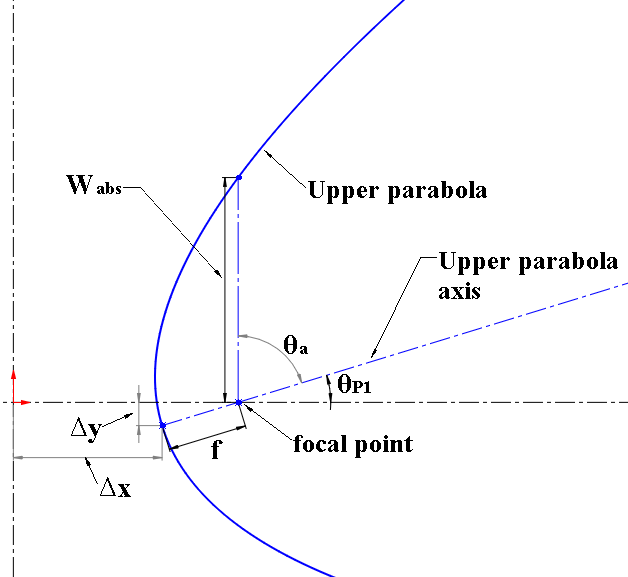
\includegraphics[width=0.9\columnwidth,height=6.0cm]{figs/upper_parabola.PNG}
		\subcaption{Upper parabola.}
	\end{minipage}
	\begin{minipage}{0.49\columnwidth}
		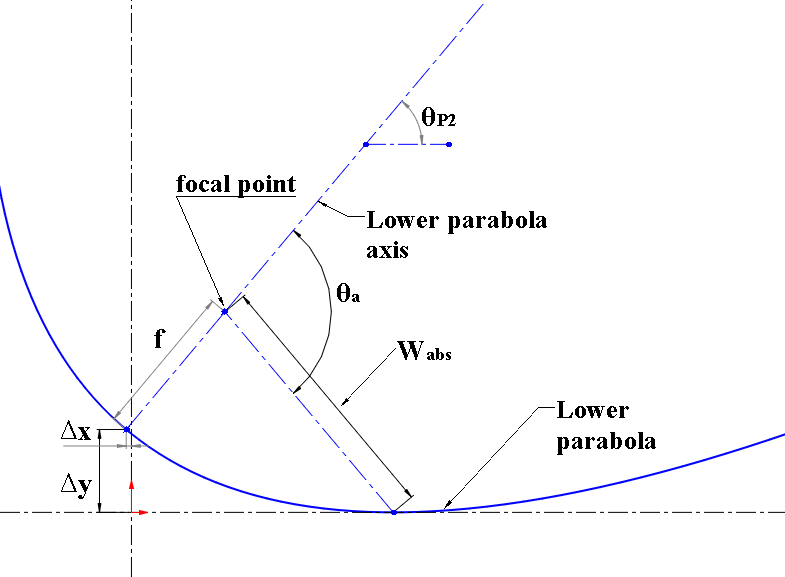
\includegraphics[width=0.9\columnwidth,height=6.0cm]{figs/lower_parabola.PNG}
		\subcaption{Lower parabola.}
	\end{minipage}
	\caption{(a) Upper and (b) lower parabolas placed at the final position.}
	\label{rottrans_two}
\end{figure}

\begin{table}[!ht]
	\centering
	\caption{Expressions for the parabolas' parameters.}
	\begin{tabular}{cp{3.3cm}l}
		\hline \\[-12pt]
		\vspace*{0.1cm} Parameter & Upper Parabola & Lower Parabola \\ [0pt]
		\hline \\[-12pt]
		$\theta_{{\rm{a}}}$ & $90 -\theta_{\!_{\rm{P1}}}$ & 2$\theta_{\!_{\rm{P2}}}$ \\ [5pt]
		%$\theta_{\!_{\rm{R}}}$ & 90 $- \alpha_{\!_{\rm{P1}}}$ & 90 $- \alpha_{\!_{\rm{P2}}}$ \\ [5pt]
		$\Delta \rm{x}$ & $\rm{{W_{abs}} - f\cos {\theta_{\!_{P1}}}}$ & $\rm{{W_{abs}} - ({W_{abs}} + f)\cos {\theta_{\!_{P2}}}}$ \\ [5pt]
		$\Delta \rm{y}$ & $\rm{- f\sin {\theta_{\!_{P1}}}}$ & $\rm{({W_{abs}} - f)\sin {\theta_{\!_{P2}}}}$ \\ 
		\hline 
	\end{tabular}
	\label{parabolas}
\end{table}

\newpage
The next step was to arrange the parabolas properly in a common coordinate system to form the full untruncated parabolic section shape APQD, shown in Figure \ref{twoparabolas22}. In this case, point D intercepts the x-axis and the vertical segment length AD equals $\rm{W_{abs}}$, the section end. The full aperture indicated by the segment PQ is obtained according to the angles of the parabola axes. The aperture was set to be vertical; therefore, the section is truncated at the line indicated by segment BC. The AB and DC curves represent the shapes of the upper and lower reflectors, respectively. Their coordinate limits are given in Table \ref{coordinates}.

\Figure[scale=0.55,placement=!ht,label={twoparabolas22},caption={Two parabolas arranged to form the truncated parabolic section (ABCD). Dashed curves of the parabolas were eliminated.},shortcaption={Two parabolas assembled to form the truncated parabolic section (ABCD)}]{figs/fig_primary3.PNG}

\begin{table}[!ht]
	\centering
	\caption{Reflector coordinate limits.}
	\begin{tabular}{lll}
		\hline \\[-12pt]
		\vspace*{0.1cm} Reflector & x limits & y limits \\ [0pt]
		\hline \\[-12pt]
		Upper & $\rm{{W_{abs}} \le {x} \le {x_{apt}}}$ & $\rm{{W_{abs}} \le {y} \le {y_{apt,upper}}}$ \\ [5pt]
		Lower & $\rm{{W_{abs}} \le {x} \le {x_{apt}}}$ & $\rm{0 \le {y} \le {y_{apt,lower}}}$ \\ 
		\hline 
	\end{tabular}
	\label{coordinates}
\end{table}

%The mathematical process of rotation and translation was achieved using the Affine transformation technique (\cite{Duffy2016}), which consists of applying a matrix multiplication as shown in Eq. (\ref{affine}):
%
%\begin{equation}
%\left[ {\begin{array}{*{20}{c}}
%		\mathrm{{{x }}}\\
%		\mathrm{{{y }}}\\
%		1
%		\end{array}} \right] = \left[ {\begin{array}{*{20}{c}}
%		1&0&\mathrm{\Delta x}\\
%		0&1&\mathrm{\Delta y}\\
%		0&0&1
%		\end{array}} \right]\left[ {\begin{array}{*{20}{c}}
%		\mathrm{\cos {\theta_{\!_R}}}&\mathrm{\sin {\theta_{\!_R}}}&0\\
%		\mathrm{- \sin {\theta_{\!_R}}}&\mathrm{\cos {\theta_{\!_R}}}&0\\
%		0&0&1
%		\end{array}} \right]\left[ {\begin{array}{*{20}{c}}
%		\mathrm{{{ x_p }}}\\
%		\mathrm{{{ y_p }}}\\
%		1
%		\end{array}} \right]
%\label{affine}
%\end{equation}
%
%\noindent with the parameters $\rm{\Delta x}$ and $\rm{\Delta y}$ as the displacements in x and y, respectively, $\rm{\theta_{\!_R}}$ as the angle of rotation (which is the complement of the parabola axis angle), and $\rm{{{x}}}$ and $\rm{{{y}}}$ are the new coordinates of the parabola calculated by the Affine transformation technique. 
%
%The mathematical equation to represent a rotated-translated parabola is implicit defined by an irreducible polynomial of second degree, which is complex solve for ray tracing applications. Another way of representing the portion of the parabolic reflectors was thus used to approximate the parabolic shapes to a $\rm{N_d}^{\rm{th}}$ degree polynomial fit  in the form of:
%
%\begin{equation}
%\mathrm{y = \sum\limits_{j = 0}^{N_d} {{a_j}x^j}}
%\label{eqP1}
%\end{equation}
%
%\noindent where the linear coefficients $\rm{a_{\!_{0}}}$, $\rm{a_{\!_{1}}}$, $\rm{a_{\!_{2}}}$, $\rm{a_{\!_{3}}}$, ..., $\rm{a_{\!_{Nd}}}$ and the degree order $\rm{N_d}$ were determined in a way to maximise the fit using a linear least-squares solver with linear constraints.

The equations used to model the parabolas consider x and y as functions of a new parametric variable $\rm{t_p}$ assigned for each parabolic shape, as shown in Eqs. (\ref{p_x}) and (\ref{p_y}). These parametric equations model the exact parabolic shapes and are quadratic polynomials in $\rm{t_p}$, which takes minimum process time to be solved. 

\begin{equation}
	\mathrm{x = \frac{1}{4f}\sin\theta_a t_{p}^2 + \cos\theta_a t_p + \Delta x}
	\label{p_x}
\end{equation}
\vspace*{-0.75cm}
\begin{equation}
	\mathrm{y = \frac{1}{4f}\cos\theta_a t_{p}^2 - \sin\theta_a t_p + \Delta y}
	\label{p_y}
\end{equation}

\noindent where the parametric variables range to provide x and y coordinates whose limits are established in Table \ref{coordinates}.

\subsection{Circular reflector design}

A quarter of a circle was used for the circular reflector, whose centre was set at \mbox{($\rm{W_{abs}}$, $\rm{W_{abs}}$)} and radius $\rm{W_{abs}}$. Eq. (\ref{quartercircle}) expresses the calculation for the circular section:

\begin{equation}
	\mathrm{{y} = {W_{abs}} - \sqrt {\mathrm{W_{abs}^2 - {{\left( {{x} - {W_{abs}}} \right)}^2}}}}
	\label{quartercircle}
\end{equation}

\noindent where the coordinate limits are $\rm{0 \le {x} \le {W_{abs}}}$ and $\rm{0 \le {y} \le {W_{abs}}}$. The shape of the circular sector is illustrated in Figure \ref{three_sections} by the curve DE. 

\subsection{Straight reflector design}

The straight reflector section comprises two vertically straight reflectors of height $\rm{H_{\!_{TS}}}$ above the circular section and ends at the absorber surface (whose y-coordinate is $\rm{y_{\!_{TS}}}$). The coordinate limits here are $\rm{0 \le {x} \le {W_{abs}}}$ and $\rm{W_{abs} \le {y} \le {y_{\!_{TS}}}}$. Figure \ref{three_sections} represents them by the vertical segments EF and AG.
%, as shown in Figure \ref{TS_SS}.

\subsection{End reflectors design}

The end reflectors are two identical flat surfaces, one at each end of the concentrator (west and east sides shown in Figure \ref{collector3D}), where their boundaries are the shapes of the other reflectors.

\subsection{Summary of overall coordinates}

Figure \ref{three_sections} illustrates all the reflectors arranged along with the main coordinates.

\Figure[scale=0.35,placement=!ht,label={three_sections},caption={Concentrator's cross-section view with the appropriate coordinate information.}]{figs/three_sections.PNG}

Figure \ref{three_sections3D} shows the concentrator in three dimensions where:

\begin{itemize}[topsep=5pt,partopsep=0pt] \itemsep0pt
\item AHIB and DKJC are the upper and lower parabolic reflectors;
\item ELKD is the circular reflector;
%\item ELMF and AHNG are the straight reflectors;
\item ABCDEFG and HIJKLMN are the western and eastern end reflectors, respectively;
\item FMNG is the absorber surface and BIJC is the aperture;
\item The concentrator’s main dimensions are: depth $\rm{W_{col}}$, height $\rm{H_{col}}$ and length $\rm{L_{col}}$.
\end{itemize}

\Figure[scale=0.55,placement=!ht,label={three_sections3D},caption={Final concentrator concept.}]{figs/collector3D-3.PNG}

\section{Ray Tracing and Optical Modelling}

The complex geometry of the IACPC makes it difficult to predict its optical performance with analytical equations. To overcome this challenge, a 3D ray tracing algorithm in Matlab was used to simulate direct solar radiation entering through the aperture, reflecting off the reflectors, and reaching the absorber. Figure \ref{triad} illustrates a 3D coordinate system used to represent the geometry of a ray in space. It defines a vector with its initial point $\rm{(x_0, y_0, z_0)}$ from which the ray originates and a point of incidence $\rm{(x_{\text{int}}, y_{\text{int}}, z_{\text{int}})}$ where the ray intersects the surface. It is also defined by its angular components  $\theta_{iy}$ and  $\theta_{iz}$. The diagram describes a ray's spatial orientation in the system's context.

\begin{figure}[!ht]
	\centering
	\begin{tikzpicture}[scale=5,tdplot_main_coords,very thick,framed]
		\coordinate (O) at (0,0,0);
		\tdplotsetcoord{P}{\rvec}{\thetavec}{\phivec};
		\draw[arrow] (0,0,0) -- (0.75,0,0) node[anchor=north east]{x (south)};
		\draw[arrow] (0,0,0) -- (0,0.75,0) node[anchor=north west]{z (east)};
		\draw[arrow] (0,0,0) -- (0,0,0.75) node[anchor=south]{y (up)};
		\draw[arrow,color=red] (P) node[anchor=west]{\color{black}Initial point ($\rm{x_0,y_0,z_0}$)} -- (O) node[anchor=east]{\color{black}Point of incidence ($\rm{x_{int},y_{int},z_{int}}$)};
		\draw[dashed, color=red] (O) -- (Pxy);
		\draw[dashed, color=red] (P) -- (Pxy);
		\tdplotdrawarc{(O)}{0.2}{0}{\phivec}{anchor=north}{$\rm{\theta_{iz}}$}
		\tdplotsetthetaplanecoords{\phivec}
		\tdplotdrawarc[tdplot_rotated_coords]{(O)}{0.25}{90}{\thetavec}{anchor= south west}{$\rm{\theta_{iy}}$}
	\end{tikzpicture}
	\caption{Orientation in 3D of one incoming ray going through the concentrator.}
	\label{triad}
\end{figure}

The flowchart in Figure \ref{flow-opt} outlines how to trace a ray through the concentrator and determine its optical efficiency. The process begins by defining the concentrator's boundaries and initialising the ray's path. As the ray is traced, intersections with the concentrator's reflectors -- such as the ends, parabolic surfaces, and straight segments -- are checked. Each intersection adds a reflection to the ray's path. The total number of reflections is summed if the ray reaches the absorber, and the optical efficiency is determined. If the ray fails to reach the absorber, it is rejected, and the optical efficiency is set to zero. The process ends when the efficiency is calculated, or the ray is rejected.

%\singlespacing
\begin{figure}[!ht]
	\centering
	\scalebox{0.8}[0.8]{
		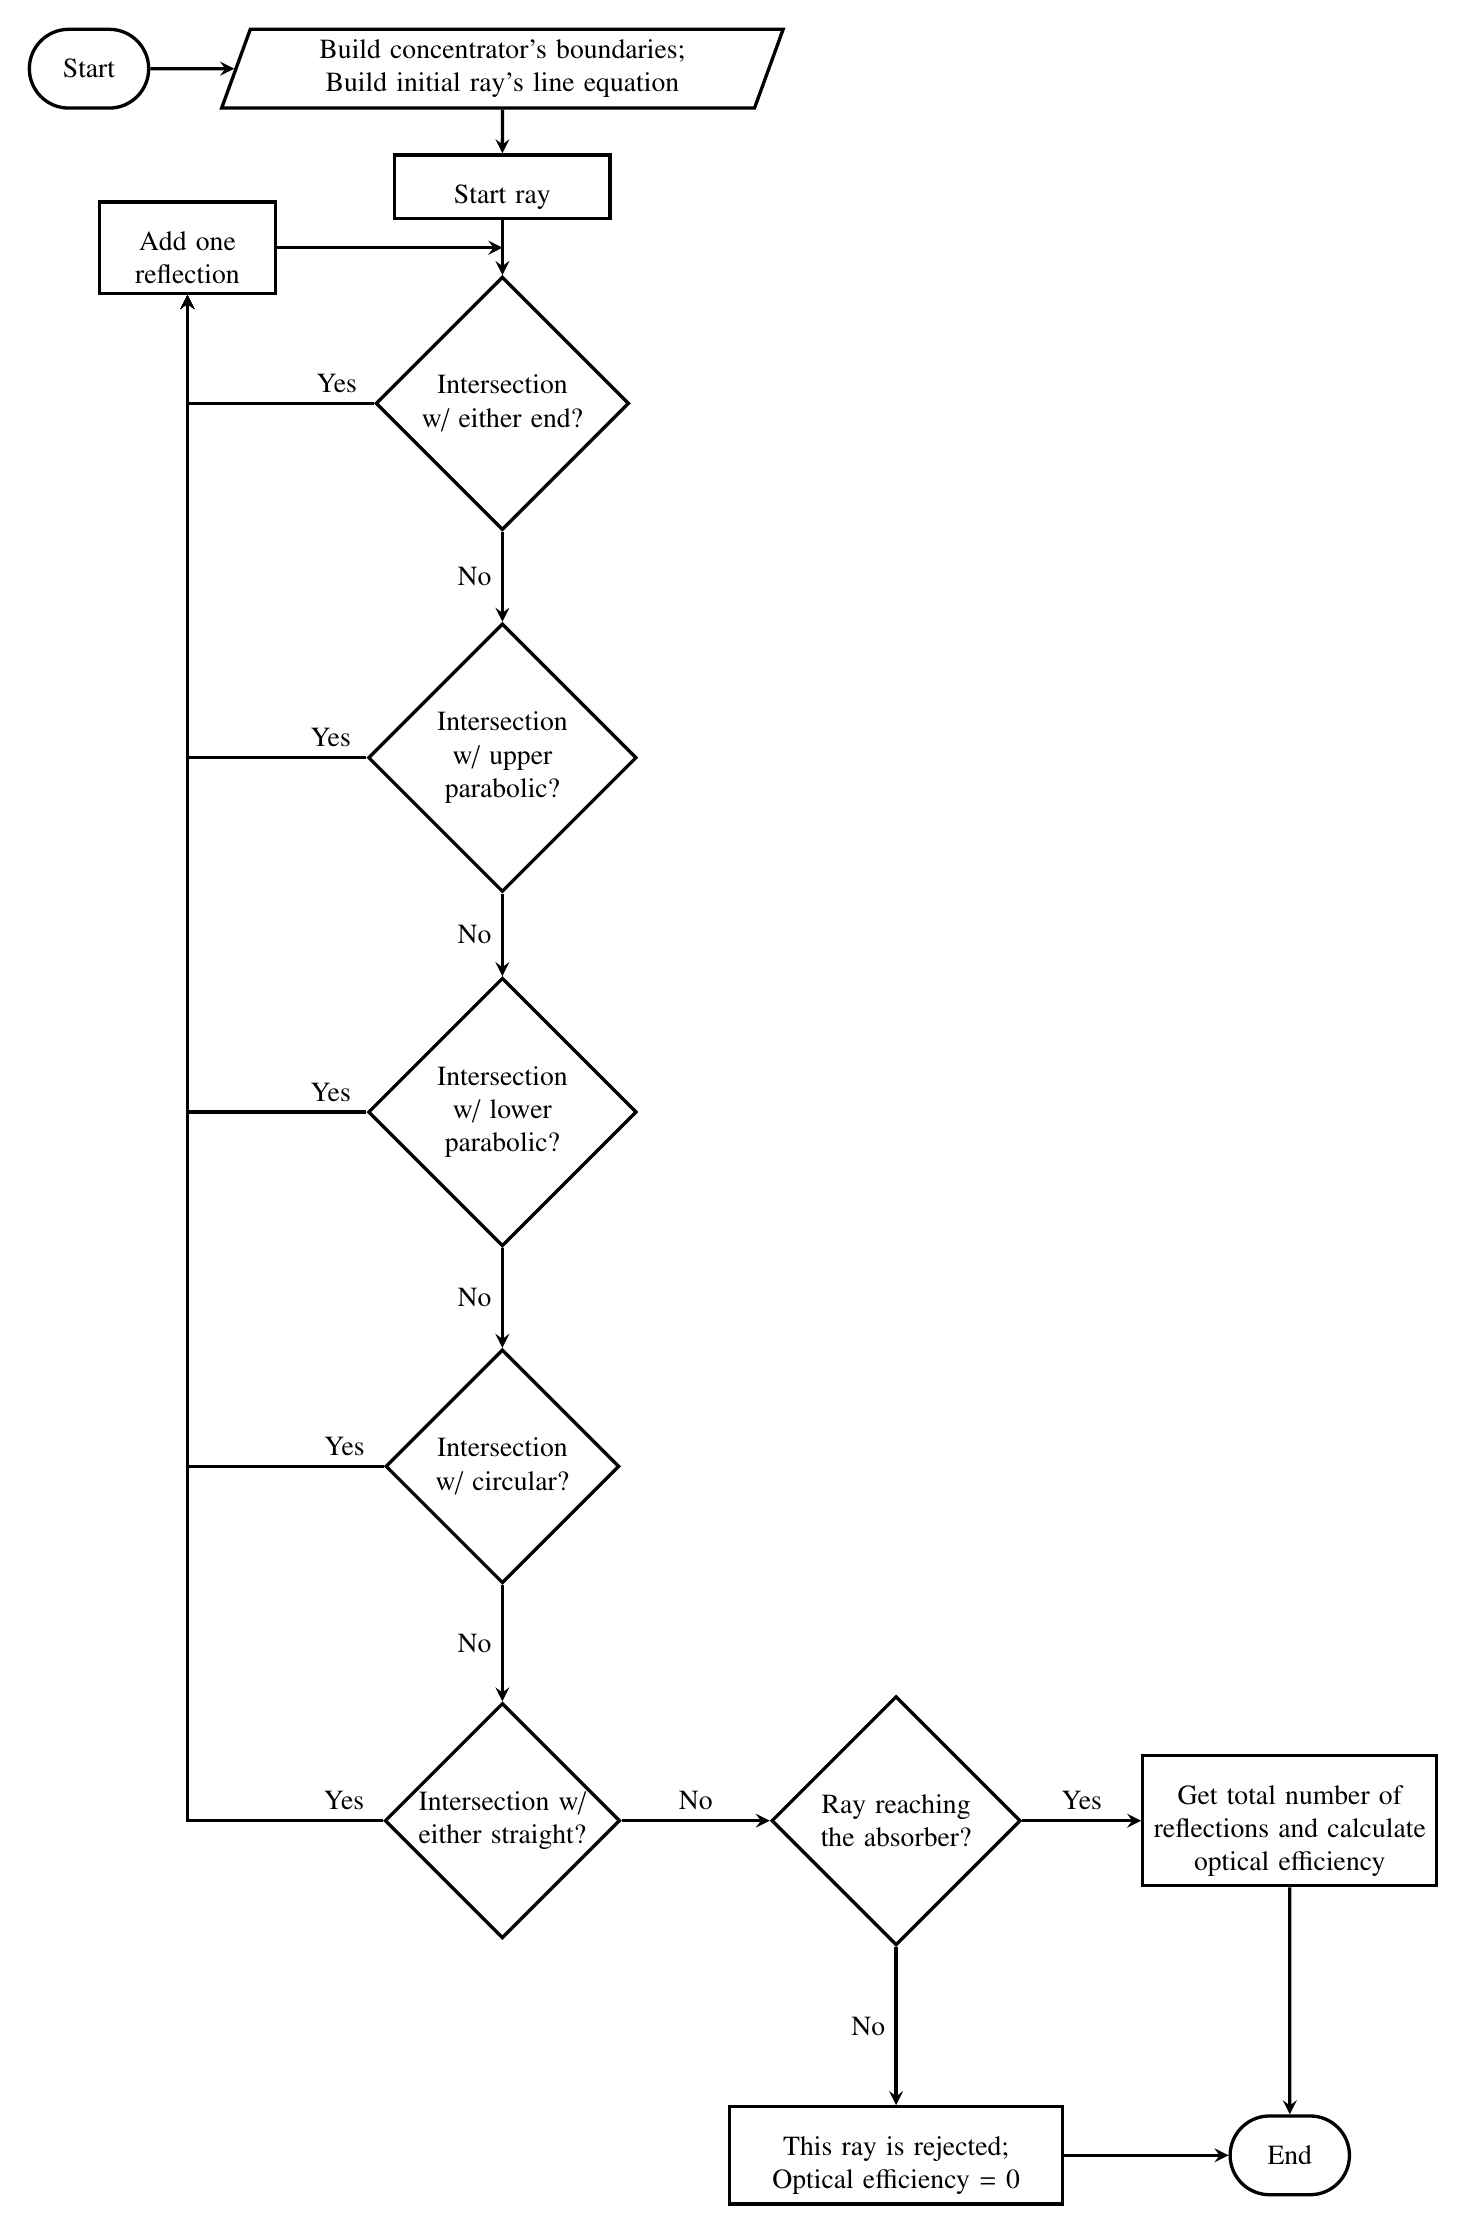
\begin{tikzpicture}[node distance = 3cm]
			\node[startstop,xshift=-1cm] (start) {Start};
			\node[input, right of=start,text width=6cm] (init) {Build concentrator's boundaries; Build initial ray's line equation};
			\node[block, below of=init, text width=4cm,yshift=1.5cm,text width=2.5cm] (new) {Start ray};
			\node[decision, below of =new,yshift=0.75cm] (rend) {Intersection w/ either end?};
			\node[decision, below of = rend,yshift=-1cm,text width = 2.25cm] (rupper) {Intersection w/ upper parabolic?};
			\node[decision, below of = rupper,yshift=-1cm,text width = 2.25cm] (rlower) {Intersection w/ lower parabolic?};
			\node[decision, below of = rlower,yshift=-1cm,text width = 2.25cm] (rcirc) {Intersection w/ circular?};
			\node[decision, below of = rcirc,yshift=-1cm,text width = 2.25cm] (rstr) {Intersection w/ either straight?};
			\node[decision, right of = rstr,xshift=1.5cm] (abs) {Ray reaching the absorber?};
			\node[block, right of=abs,xshift=2cm,text width=3.5cm] (calc) {Get total number of reflections and calculate optical efficiency};
			\node[startstop,below of=calc,yshift=-1.25cm] (end) {End};
			\node[block, below of=abs,yshift=-1.25cm,text width=4cm] (rej) {This ray is rejected; Optical efficiency = 0};
			
			\draw[arrow] (start) -- (init);
			\draw[arrow] (init) -- (new);
			\draw[arrow] (new) -- coordinate[midway](m1)(rend);
			\node[block, left of=m1,xshift=-1cm] (ref) {Add one reflection};
			\draw[arrow] (ref) -- (m1);
			\draw[arrow] (rend) -| coordinate[pos=0.1](m2) (ref); \node [black,above=0.01 of m2] {Yes};
			\draw[arrow] (rend) -- node[anchor=east] {No} (rupper);
			\draw[arrow] (rupper) -| coordinate[pos=0.1](m3) (ref); \node [black,above=0.01 of m3] {Yes};
			\draw[arrow] (rupper) -- node[anchor=east] {No} (rlower);
			\draw[arrow] (rlower) -| coordinate[pos=0.1](m4) (ref); \node [black,above=0.01 of m4] {Yes};
			\draw[arrow] (rlower) -- node[anchor=east] {No} (rcirc);
			\draw[arrow] (rcirc) -| coordinate[pos=0.1](m5) (ref); \node [black,above=0.01 of m5] {Yes};
			\draw[arrow] (rcirc) -- node[anchor=east] {No} (rstr);
			\draw[arrow] (rstr) -| coordinate[pos=0.1](m6) (ref); \node [black,above=0.01 of m6] {Yes};
			\draw[arrow] (rstr) -- node[anchor=south] {No} (abs);
			\draw[arrow] (abs) -- node[anchor=south] {Yes} (calc);
			%\draw[arrow] (calc) -- (next);
			%\draw[arrow] (next) |- coordinate[pos=0.01](m7) (m1); \node [black,left=0.01 of m7] {Yes};
			%\draw[arrow] (abs) |- coordinate[pos=0.1](m8) (rej); \node [black,left=0.01 of m8] {No};
			%\draw[arrow] (rej) -| (next);
			%\draw[arrow] (next) -- node[anchor=south] {Yes} (opt);
			\draw[arrow] (abs) -- node[anchor=east] {No} (rej);
			\draw[arrow] (calc) -- (end);
			\draw[arrow] (rej) -- (end);
		\end{tikzpicture}
	}
	
	\caption{Flowchart of the algorithm to execute the optical modelling.}
	\label{flow-opt}
\end{figure}

\doublespacing



%\Figure[scale=0.60,placement=!ht,label={orientation},caption={Concentrator's orientation in the space and one incoming ray going through the aperture.},frame]{figs/orientation.eps}

%\newpage
The following assumptions were made in the algorithm development:

\begin{itemize} [topsep=5pt,partopsep=0pt] \itemsep0pt
\item All reflectors are specular so the incident angle is equal to the reflected angle to the normal at the intersection point;
\item A density of 1 ray per mm$^{\rm 2}$ of aperture was initially placed on the surface, with rays distributed evenly. Each ray carried equal energy, independent of the solar altitude and azimuth angles. While higher ray densities were tested, they showed no significant impact on optical efficiency and only increased computing power;
\item The boundaries are the reflective surfaces shown in Figure \ref{three_sections3D}, where the rays go through the face BIJC.
\end{itemize}

The 2D ray tracing is only the particular case of the 3D ray tracing, at which the azimuth solar angle is zero. For all the 2D simulations, there are no reflections at the end reflectors. Figure \ref{RT-diagram} illustrates rays entering the concentrator and getting reflected until reaching the absorber in 2D and 3D, respectively.

\begin{figure}[ht!]
	\begin{minipage}{0.49\columnwidth}
		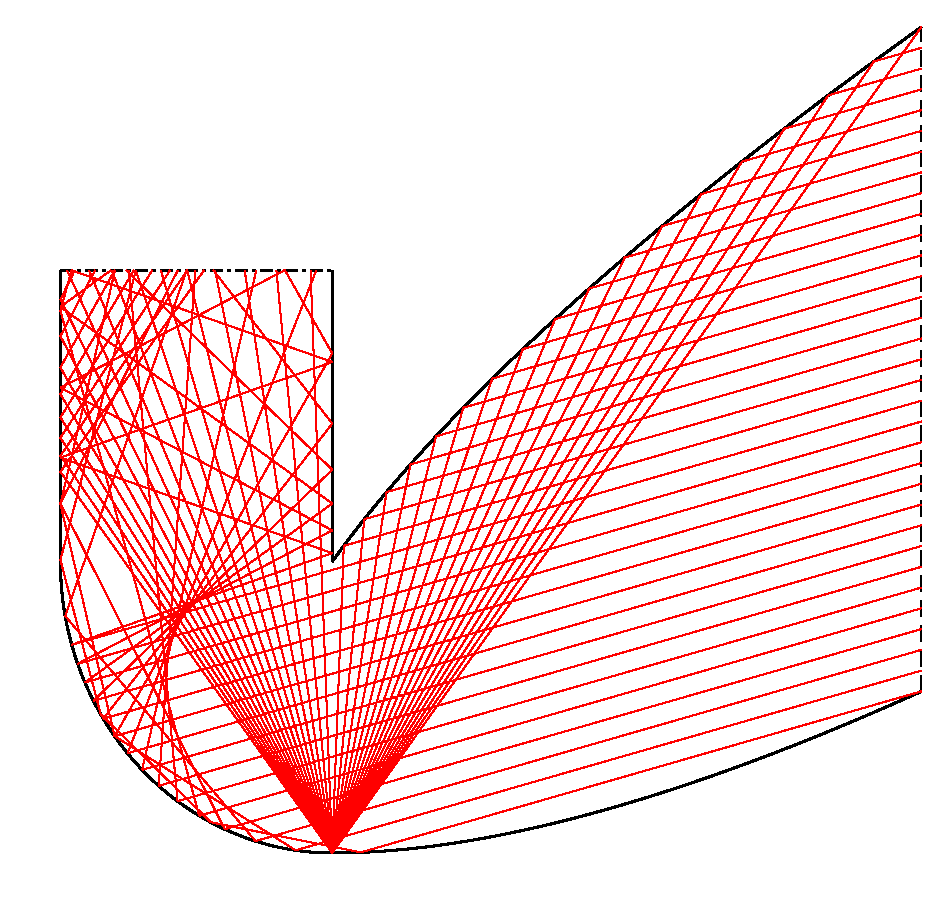
\includegraphics[width=0.90\columnwidth,height=5cm]{figs/2D-diagram-15.eps}
		\subcaption{2D RT diagram at $\rm{a_s = 15^o}$.}
		
		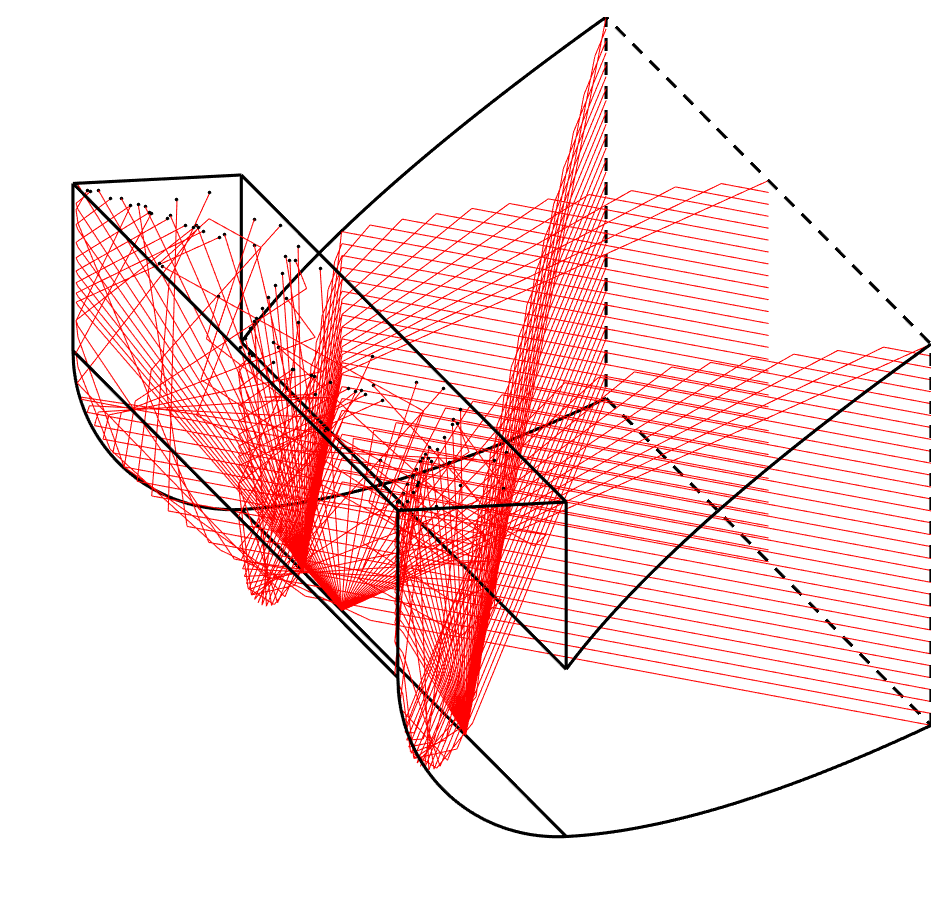
\includegraphics[width=0.95\columnwidth,height=5.5cm]{figs/3D-diagram-15.eps}
		\subcaption{3D RT diagram at $\rm{a_s = 15^o}$ and $\rm{\gamma_s = 70^o}$.}
	\end{minipage}
	\begin{minipage}{0.49\columnwidth}
		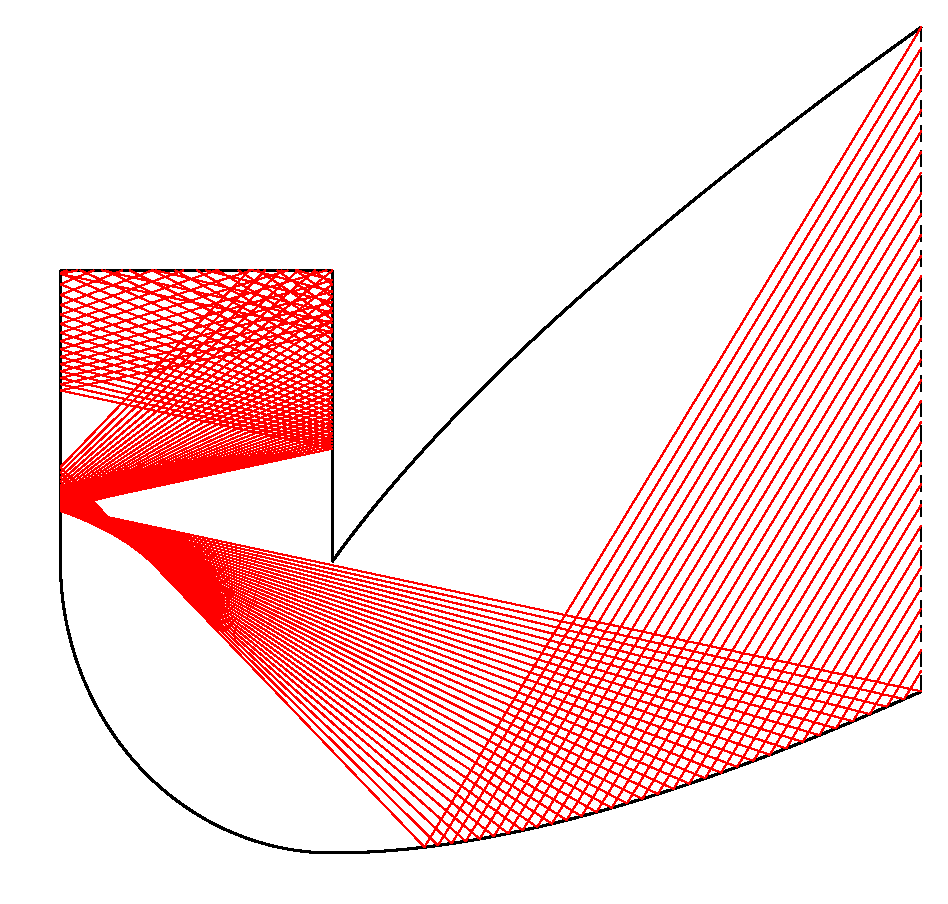
\includegraphics[width=0.90\columnwidth,height=5cm]{figs/2D-diagram-60.eps}
		\subcaption{2D RT diagram at $\rm{a_s = 60^o}$.}
		
		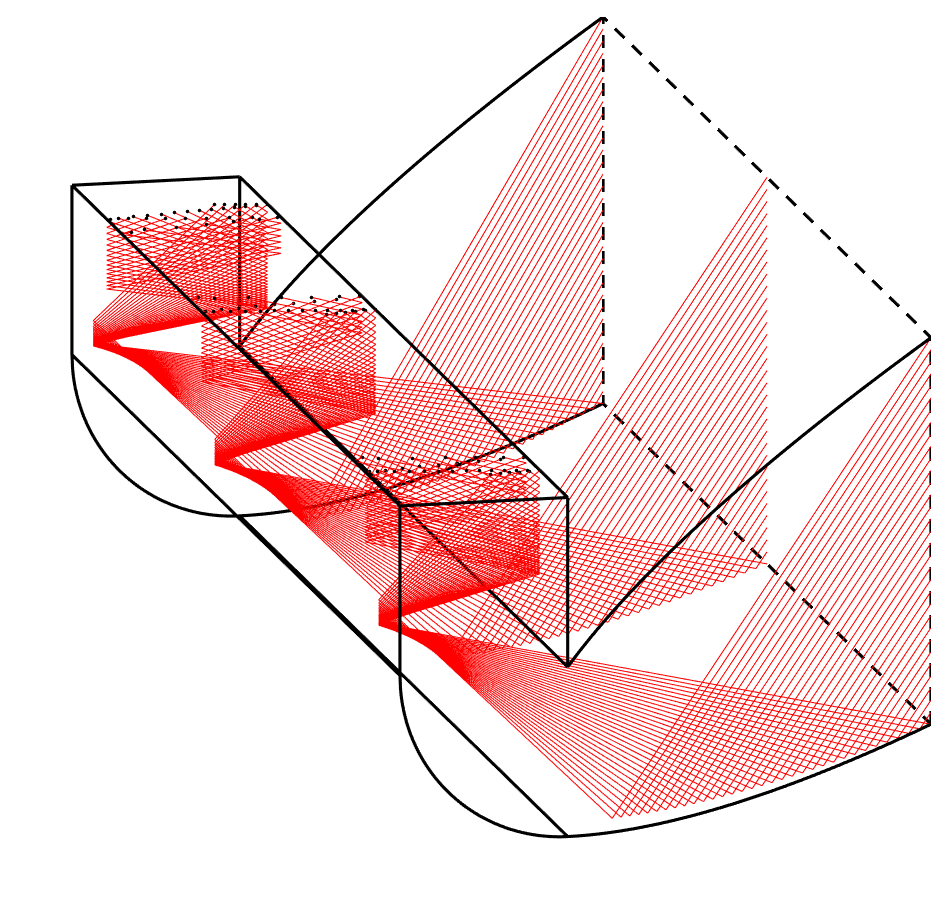
\includegraphics[width=0.95\columnwidth,height=5.5cm]{figs/3D-diagram-60.eps}
		\subcaption{3D RT diagram at $\rm{a_s = 60^o}$ and $\rm{\gamma_s = 10^o}$.}
		
	\end{minipage}
	\caption{Ray tracing diagrams in 2D and 3D.}
	\label{RT-diagram}
\end{figure}

%The glazing transmittance $\tau_{\rm{g}}$, calculated using equations described in \citet{Duffie2013}, is dependent of the inclination $\beta$, which affects the incident angle $\theta_{\rm{i}}$, defined as the angle between the incident solar ray and the normal to the glazing, is calculated by Eq. (\ref{incidence}):
%
%\begin{equation}
%\mathrm{\theta_i = {\cos ^{-1}}\left[ {\cos {a_s}\cos ({\gamma_s} - {\gamma_w})\sin \beta  + \sin {a_s}\cos \beta} \right]}
%\label{incidence}
%\end{equation}
%
%\noindent where $\gamma_{\rm{s}} = 0$ in the 2D analysis, and the concentrator azimuth angle $\gamma_{\rm{w}}$ is zero as the system is south facing.

The optical efficiency is defined as the ratio between the absorbed and the incident solar energy. Considering the number of reflections, glazing transmittance and absorber absorptance, it is calculated using Eq. (\ref{optical}) as a function of the reflectors' shape, the concentration ratio and the incident angle $\theta_{\rm i}$ from Eq. (\ref{incidence0}) (\cite{Sellami2013}):

\vspace{-0.75cm}
\begin{equation}
\mathrm{\eta_o = {\mathlarger{\sum\limits}_{\scriptscriptstyle i=1}^{\scriptscriptstyle \mathrm{N_{rays}}}{{\rho_{ref}^{{r_i}}}}}\tau_{glaz}\alpha_{abs}}
\label{optical}
\end{equation}

\noindent where $\rm{r_i}$ is the number of reflections of the solar ray i.

The effective concentration ratio ($\rm{C_{eff}}$), which is the product of the geometric concentration ratio and the optical efficiency, is given by Eq. (\ref{Ceff}). $\rm{C_{eff}}$ is useful to select shapes capable of enhancing both concentration of energy at the absorber and optical efficiency. All the optical outputs $\tau_{\rm {glaz}}$, $\eta_{\rm o}$ and $\rm{C_{eff}}$ can be calculated as averaged values to represent the whole period of operation for each particular concentrator. They were called $\tau_{\rm glaz,avg}$, $\eta_{\rm o,avg}$ and $\rm{C_{eff,avg}}$.

\vspace{-0.75cm}
\begin{equation}
\mathrm{C_{eff} = \eta_{\!_o}CR}
\label{Ceff}
\end{equation}

The collector's dimensions can also be related as dimensionless relative to the absorber width: $\rm{W^{*} = W_{col}/W_{abs}}$, $\rm{H^{*} = H_{col}/W_{abs}}$ and $\rm{L^{*} = L_{col}/W_{abs}}$. The dimensionless parameter A$^*$ was introduced to consider the reflector area relative to the absorber area, where:

\vspace{-0.75cm}
\begin{equation}
\mathrm{{A^*} = \frac{{{A_R}}}{{{A_{abs}}}} = \frac{{{W_r}}}{{{W_{abs}}}} + 2\frac{{{W^*}{H^*}}}{{{L^*}}}}
\label{reflectorarea}
\end{equation}

\noindent where $\rm{W_{ref}}$ (m) is the width of reflective material employed for a particular shape.

\section{Results and Discussion}

\subsection{Overview and collector specification}

This section was organised as follows:

\begin{itemize}[topsep=5pt,partopsep=0pt] \itemsep0pt
\item Design analysis of a standalone collector's geometry using the dimensionless parameters W$^{*}$, H$^{*}$ and A$^{*}$ at different parabolic shapes as a function of the truncation level (in terms of the geometric concentration ratio CR);
\item Optical performance considering the average values of optical efficiency $\rm{\eta_o}$ and effective concentration ratio $\rm{C_{eff}}$ at different shapes (in terms of $\theta_{\!_{\rm{P2}}}$) as a function of CR at a fixed absorber width, zero tertiary section height ($\rm{H_{TS} = 0}$) and $\rm{L_{col} = 10W_{abs}}$, 
\item Optical performance of two different geometries by varying the length;
\item Selection of the collector for further fabrication;
\item Evaluation of the cavity height on the optical efficiency and the energy distribution over the absorber;
\item Optical characterisation of the collector.
%\item Comparison of the combination of three different concentrator shapes on a fixed area of wall;
%\item Evaluation of the effect of the aperture size of the same collector at a fixed length;
%\item Analysis of different combinations in terms of aperture size at a fixed area of wall.
\end{itemize}

%\subsection{Collector specification}

An optical analysis was conducted for the solar air heating collector with the following specifications:

\begin{itemize} [topsep=5pt,partopsep=0pt] \itemsep0pt
    \item The absorber absorptance ($\alpha_{\rm{abs}}$) is 0.85;
    \item The reflector reflectance ($\rho_{\rm{ref}}$) is 0.95;
    \item A 4-mm thick low iron glass was employed with a refractive index of 1.526 and an extinction coefficient of 4 m$^{\!^{-1}}$. When the rays are perpendicular to the surface, the value of $\tau_{\rm{glaz}}$ is 0.90;
    \item The maximum truncation level was set to result in the minimum geometric concentration ratio of 2.0 regardless of the parabolic shape.
    \item The upper parabola axis angle was set to be coincident with the lowest solar altitude angle ($\theta_{\!_{\rm{P1}}}$ = 15$^{\circ}$);
    \item The range of lower parabola axis angles ($\theta_{\!_{\rm{P2}}}$) was between 44$^{\circ}$ and 61$^{\circ}$.
\end{itemize}

\subsection{Effect of the glazing inclination on the transmittance}

The glazing transmittance $\tau_{\rm{glaz}}$ varies in relation to the incident angle $\theta_{\rm{i}}$ as shown in Figure \ref{transm}. It was calculated using Eqs. (\ref{snell}), (\ref{rho_glaz}), (\ref{abs_glaz}) and (\ref{transmi}). The value of $\tau_{\rm{glaz}}$ is approximately 0.9 for incident angles lower than 40$^{\circ}$.

\Figure[scale=0.60,placement=!ht,label={transm},caption={Transmittance as function of the angle of incidence.}]{figs/transm.eps}

\newpage
The average transmittance calculated as a function of the glazing inclination is shown in Figure \ref{transmittance}. A maximum average transmittance is at \mbox{$\beta$ = 33$^{\circ}$} as 0.8907, thus is the inclination of which the glazing losses are minimum overall. Compared to the transmittance with the glazing placed vertically, there is a relative difference of 14\%. However, an inclination at $\beta$ = 33$^{\circ}$ brings practical difficulties, such as a high dust accumulation and rainwater over the glazing cover. For this reason, a steeper inclination was desirable, even though less solar energy is reaching the absorber. Therefore, \mbox{$\beta$ = 62$^{\circ}$} was chosen, where \mbox{$\tau_{\rm{g,avg}}$ = 0.8770}, more than 98\% of the maximum average transmittance.

\Figure[scale=0.60,placement=!ht,label={transmittance},caption={Average transmittance dependent on glazing inclination.}]{figs/transmittance.eps}

The results of instantaneous light transmittance against daytime is shown in Figure \ref{transm-time} for different glazing inclinations on 30$^{\rm th}$ June. The maximum transmittance profile is at $\beta$ = 33$^{\circ}$, whereas the one of inclination at the local latitude angle ($\beta$ = 53$^{\circ}$) and the one at $\beta$ = 62$^{\circ}$ do not present a significant difference. All three profiles are similar between 11:00 and 16:00 on this day. On the other hand, the vertical glazing profile shows the highest amount of solar reflection.

\Figure[scale=0.55,placement=!ht,label={transm-time},caption={Light transmittance throughout the day (30$^{\rm th}$ June).}]{figs/transm-time.eps}

\subsection{Design analysis of standalone collectors}

The dimensionless parameters $\rm{W^{*}}$ and $\rm{H^{*}}$ are presented by graphs in Figure \ref{size_region2}, where each graph corresponds to a particular shape. The maximum concentration ratio, obtained from the shape at $\theta_{\!_{\rm{P2}}} = 44^{\circ}$, was 2.98. $\rm{W^{*}}$ and $\rm{H^{*}}$ decrease as $\theta_{\!_{\rm{P2}}}$ increases for the same concentration ratio because the concentrator's acceptance angle is broader. For the same concentrator (fixed shape), the size increases when CR increases until its maximum aperture width, thus defining its maximum size (indicated by the dashed line in Figure \ref{size_region2}). The smallest concentrator has the shape of the narrowest acceptance angle ($\theta_{\!_{\rm{P2}}} = 44^{\circ}$) and the smallest concentration ratio (CR = 2.0) for being the most truncated ($\rm{W_{col} = 2.2W_{abs}}$ and $\rm{H_{col} = 2.2W_{abs}}$). In contrast, the largest concentrator has the narrowest acceptance angle but at the highest concentration ratio ($\rm{W_{col} = 7.3W_{abs}}$ and $\rm{H_{col} = 5.4W_{abs}}$). 

\Figure[scale=0.70,placement=!ht,label={size_region2},caption={Dimensionless parameters $\rm{W^{*}}$ and $\rm{H^{*}}$ matching particular CR for different shapes.}]{figs/size_region2.eps}

As shown in Figure \ref{reflector_region}, the dimensionless parameter $\rm{A^{*}}$ increases as the concentrator's size increases. Thus the graphs in Figures \ref{size_region2} and \ref{reflector_region} are similar. The reflector area varied from $\rm{5.4A_{abs}}$ for the smallest concentrator to nearly $\rm{24A_{abs}}$ for the largest one. Because this collector is an asymmetric compound parabolic concentrator, these graphs are similar to those found by \citet{Rabl1976} for symmetric concentrators.

\Figure[scale=0.70,placement=!ht,label={reflector_region},caption={Dimensionless parameter $\rm{A^{*}}$ matching particular CR for different shapes.}]{figs/reflector_region.eps}

%\Figure[scale=0.80,placement=!ht,label={size_region3},caption={Dimensionless parameter $\rm{A^{*}}$ matching particular CR for different shapes.}]{figs/size_region3.eps}

\subsection{Optical performance of standalone collectors}

\subsubsection{Optical performance by varying parabolic shape and truncation level}

The average optical efficiency as a function of CR for different shapes is shown in Figure \ref{eff_region2}. For concentrators of concentration ratio below 2.2, the shape of the highest optical efficiency is the one of $\theta_{\!_{\rm{P2}}} = 44^{\circ}$. For truncation levels resulting in a concentration ratio above 2.4, concentrators cannot accept a portion of direct solar radiation of solar altitude angles ($\rm{a_s}$) above 50$^{\circ}$, which is the reason why the graphs have decaying behaviours. The shape of $\theta_{\!_{\rm{P2}}} = 44^{\circ}$ and CR = 2.0 is the most efficient with $\rm{\eta_{o,avg} = 0.689}$ for being the smallest concentrator that accepts all direct solar radiation in the period of operation. The least efficient concentrator is the one of maximum CR ($\rm{\eta_{o,avg} = 0.432}$) because it requires more reflections for the solar rays to reach the absorber, and it does not accept direct solar radiation above $\rm{50^{\circ}}$ of $\rm{a_s}$, which is equivalent to 35\% of the period of operation.

\Figure[scale=0.67,placement=!ht,label={eff_region2},caption={$\rm{\eta_{o,avg}}$ matching particular CR for different shapes.}]{figs/eff_region2.eps}

The average effective concentration ratio $\rm{C_{eff,avg}}$ against CR and $\theta_{\!_{\rm{P2}}}$, is shown in Figure \ref{Ceff_region2}. Geometries of $\theta_{\!_{\rm{P2}}}$ below 56$^{\circ}$ have maximum values of $\rm{C_{eff,avg}}$ above 1.55 at each particular level of CR. After these conditions, the graphs dramatically drop as CR is increased due to the fall in optical efficiency, as discussed previously. The shape correspondent to the smallest $\rm{C_{eff,avg}}$ is the one of maximum CR ($\rm{C_{eff,avg} = 1.3}$) for being the least optically efficient; and the shape of maximum $\rm{C_{eff,avg}}$ is the one of $\theta_{\!_{\rm{P2}}} = 51^{\circ}$ and $\rm{CR = 2.5}$ although it is not able to accept direct solar radiation above $\rm{56^{\circ}}$ of $\rm{a_s}$. Concentrators of $\rm{CR = 2.0}$ are less effective in $\rm{C_{eff,avg}}$, despite being the most optically efficient concentrators.

\Figure[scale=0.65,placement=!ht,label={Ceff_region2},caption={$\rm{C_{eff,avg}}$ matching particular CR for different shapes.}]{figs/Ceff_region2.eps}

\subsubsection{Optical performance by varying concentrator length} 

The values of ${\rm \eta_{o,avg}}$ and $\rm{C_{eff,avg}}$ were calculated as a function of the dimensionless parameter $\rm{L^{*}}$ for two different concentrators: the most optically efficient (CR = 2.0) and one with the highest $\rm{C_{eff,avg}}$ (CR = 2.5). The results can be seen in Figure \ref{eff_length}. The values of ${\rm \eta_{o,avg}}$ assuming an infinite length, were 0.70 (CR = 2.0) and \mbox{0.662 (CR = 2.5)}. The end losses are higher for shorter concentrators due to more reflections. When the length is 3$\rm W_{abs}$, where $\rm \eta_{o,avg}$ is more than 95\% of the optical efficiency assuming infinite length. When $\rm{L_{col} = 10W_{abs}}$, the values of $\rm{\eta_{o,avg}}$ are more than 98\% of those assuming infinite length. Hence, a longer concentrator incurs fewer reflection losses at the ends, thus leading to higher optical efficiencies. However, the cost of additional reflective material and weight might not compensate for the little significant gain in energy collection.

\Figure[scale=0.75,placement=!ht,label={eff_length},caption={${\rm \eta_{o,avg}}$ matching particular $\rm{L^{*}}$ for two different concentrators.}]{figs/eff_length.eps}

\newpage
The end effect can be observed in more details when ${\rm \eta_{o,avg}}$ for four different length ratios are plotted against operation time. This is shown in Figure \ref{length_variance}, specifically on 30$^{\rm th}$ June for the smallest concentrator's performance (CR = 2.0). The end losses are higher in the beginning of the day due to higher values of the azimuth solar angles incurring in more reflections at the ends and therefore collectors collect less energy before noon, especially for shorter concentrators. 

\Figure[scale=0.65,placement=!ht,label={length_variance},caption={${\rm \eta_o}$ vs. time for a collector at different length ratios.}]{figs/length_variance.eps}

\subsection{Selection of the collector to be fabricated}

This topic used a criterion to select the collector's geometry to be fabricated for tests. The collector must accept solar radiation with $\rm{a_s}$ between 15$^{\circ}$ and 61$^{\circ}$. Once these limits were set, an initial design was sketched. The angles of both parabolic axes coincide with those limits, so all direct radiation within this range is accepted. From this design (shown in Figure \ref{collectors-61-50} in red), the absorber width achieved the maximum concentration ratio of 2.284. The actual aperture width ($\rm{W_{apt}}$) will be 0.33 m in order to have three collectors stacked on every metre of wall height. Hence, $\rm{W_{abs}}$ was found to be 0.145 m.

\Figure[scale=0.65,placement=!h,label={collectors-61-50},caption={Comparison between the collector at 61$^{\circ}$ of $\theta_{\!_{\rm{P2}}}$ (red) and the one at 50$^{\circ}$ (blue).}]{figs/collectors-61-50.eps}

As this collector is truncated, the range of angular acceptance may be broader than the limits previously defined. In order to validate this hypothesis, the ray tracing algorithm was used to check whether all the rays within this range were accepted. A graph of $\theta_{\rm{acc}}$ vs. ${\rm{a_s}}$ was plotted and shown in Figure \ref{acceptance}. The collector fully accepts direct radiation from 17$^{\circ}$ to 63$^{\circ}$ of ${\rm{a_s}}$, which exceeds the upper limit. Therefore, the collector's optical performance can be enhanced by further modifications to the reflectors. In this case, it was done by decreasing the lower parabola axis angle ($\theta_{\!_{\rm{P2}}}$). As this change in shape affects the number of reflections, $\rm{\eta_{\!_{o,avg}}}$ was calculated at different values of $\theta_{\!_{\rm{P2}}}$ and two graphs were plotted in Figure \ref{eff-alphaP2}. Although there is no significant gain in the average effective concentration ratio ($\rm{C_{eff,avg}}$ = 1.52) when both designs are compared, the parameter A* is reduced from 11.7 to 7.8, reducing the reflector area required by 33\%.

\Figure[scale=0.70,placement=!ht,label={acceptance},caption={Angular acceptance vs. solar altitude angle for the collector at 61$^{\circ}$ of $\alpha_{\!_{\rm{P2}}}$ (red) and the one at 50$^{\circ}$ of $\alpha_{\!_{\rm{P2}}}$ (blue).}]{figs/acceptance-graph.eps}

Furthermore, by ray tracing, the collector's angular acceptance at \mbox{$\theta_{\!_{\rm{P2}}}$ = 50$^{\circ}$} was calculated and shown in Figure \ref{acceptance} (in red). Although the full acceptance is up to 59$^{\circ}$, $\rm{\theta_{acc}}$ at 60$^{\circ}$ is above 90\%, which poorly influences the optical efficiency. From this analysis, the angles of the upper and lower parabola axes were 17$^{\rm o}$ and 50$^{\rm o}$, respectively. 

\Figure[scale=0.65,placement=!ht,label={eff-alphaP2},caption={Average optical efficiency {\itshape versus} lower parabola axis angle.}]{figs/eff-alphaP2.eps}

For the collector's length selection, the ray tracing technique was used to calculate the average optical efficiency as a function of this geometric parameter. The $\rm{\eta_{\!_{o,avg}}}$ versus $\rm{L_{col}}$ graph was plotted and shown in Figure \ref{eff-length}. For lengths above 2 m, there is little gain in efficiency (above 0.68), whereas, below this value, the reflection losses at the ends are higher, which worsens the optical performance. At $\rm{L_{col}}$ = 1.25 m, the collector's optical efficiency is 95\% of the maximum theoretical efficiency ($\rm{\eta_{\!_{o,avg}}}$ = 0.67). Therefore, this length was chosen for the collector's fabrication under optical consideration.

\Figure[scale=0.65,placement=!ht,label={eff-length},caption={Average optical efficiency {\itshape versus} collector's length.}]{figs/eff-length.eps}



\section{Optical characterisation of the proposed collector}

\subsection{Effect of the cavity height}

To understand the effect of the cavity height in the analysis, the average optical efficiency was calculated and shown in Figure \ref{opt-avg-hts} as a function of the tertiary section height. Adding a new reflective section will imply in more reflections, thus decreasing the average efficiency by approximately 3.5\%. To illustrate the effect of the tertiary section height, the collector's optical performance on 30$^{\rm th}$ June at three different heights was calculated and shown in Figure \ref{opt-eff-3hts}. The three profiles impose nearly the same efficiency from 09:00 to 10:30 and from 16:20 to 17:00. The highest difference is at 12:00, where $\eta_{\rm{o}}$ with no tertiary height is 0.71 and $\eta_{\rm{o}}$ at $\rm{H_{TS}}$ = $\rm{W_{abs}}$ is 0.61.

\Figure[scale=0.65,placement=!h,label={opt-avg-hts},caption={Average optical efficiency as function of the tertiary section height.}]{figs/opt-avg-hts.eps}

\Figure[scale=0.65,placement=!ht,label={opt-eff-3hts},caption={Optical efficiency profile for three tertiary section heights on 30$^{\rm th}$ June.}]{figs/opt-eff-3hts.eps}

Although the optical efficiency is reduced by the increase of the tertiary section height, the cavity distributes the incoming energy uniformly along the absorber surface. To demonstrate that in an example, the simulation results has the inputs: ${\rm{a_s}}$ at 54$^{\circ}$, $\gamma_{\rm{s}}$ at 0$^{\circ}$ and $\rm I_T$ at 1000~W/m$^2$. The results are shown in Figures \ref{Tertiary-hts0}, \ref{Tertiary-hts72} and \ref{Tertiary-hts145}. 

\newpage
From Figure \ref{Tertiary-hts0} with no tertiary section, a sharp peak in energy flux near the center of the absorber (close to 14 on the x-axis), with flux values exceeding 12500 W/m$^2$. The flux quickly diminishes from this central region, indicating that most of the energy is concentrated in a narrow band. All the energy is concentrated in 45 millimetres of width. 

\begin{figure}[ht!]
	\begin{minipage}{0.48\columnwidth}
		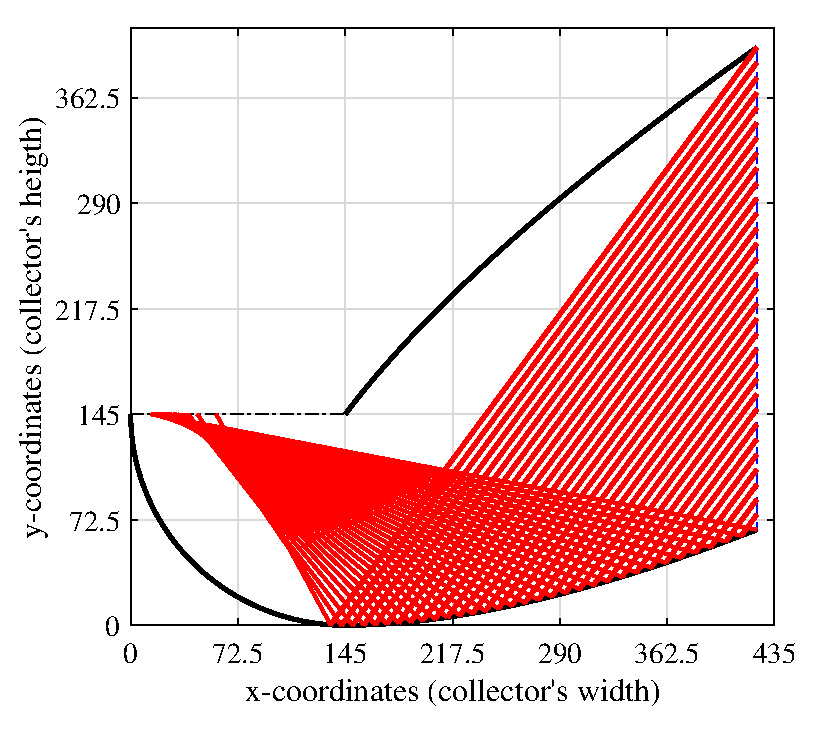
\includegraphics[scale=0.45]{figs/RT2D-hts0.eps}
		\subcaption{Ray tracing diagram (cross-section).}
		
	\end{minipage}
	\begin{minipage}{0.48\columnwidth}
		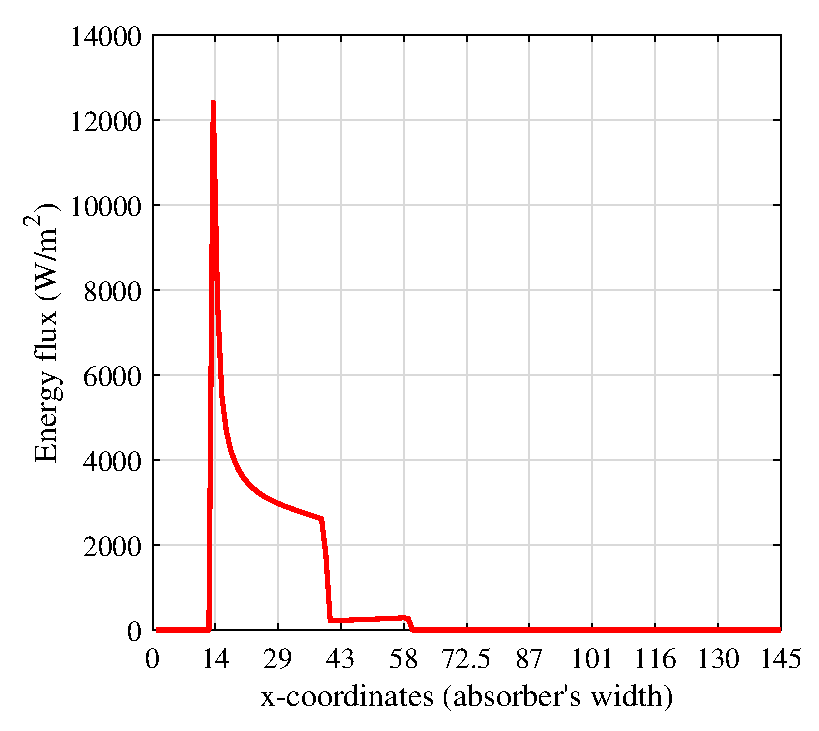
\includegraphics[scale=0.45]{figs/Energy2D-hts0.eps}
		%\\[-9mm]
		\subcaption{Energy flux distribution (cross-section).}
	\end{minipage}
	\\[3mm]
	\begin{minipage}{1.0\columnwidth}
		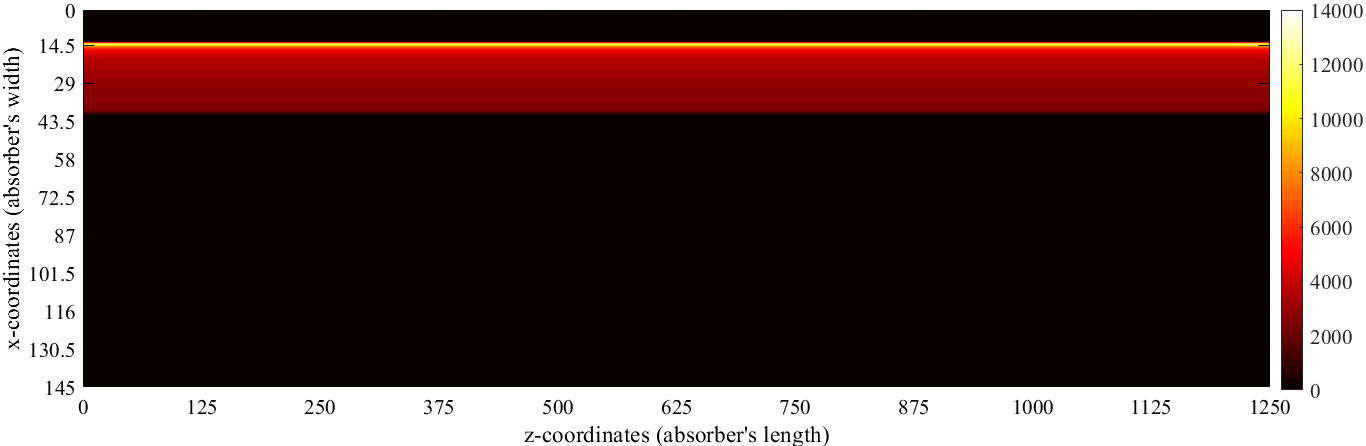
\includegraphics[scale=0.40]{figs/Energy3D-hts0.png}
		\subcaption{Energy flux distribution over the absorber surface (top view).}
	\end{minipage}
	
	\caption{Ray tracing diagram in 2D and energy flux distribution over the absorber width with no tertiary section.}
	\label{Tertiary-hts0}
\end{figure}

From Figure \ref{Tertiary-hts72} where the tertiary section height is half the width of the absorber, it can be observed that the energy flux peak is significantly reduced, reaching a maximum of 980 W/m$^2$) This represents a lower peak compared to the previous configuration shown in the earlier figure. Additionally, the decline in energy flux along the absorber width is more gradual, which implies in a smoother distribution of solar energy. It is evident that the peak region is concentrated within a narrow band of just 6 mm in width, highlighting a localised area of high intensity.

\begin{figure}[ht!]
	\begin{minipage}{0.48\columnwidth}
		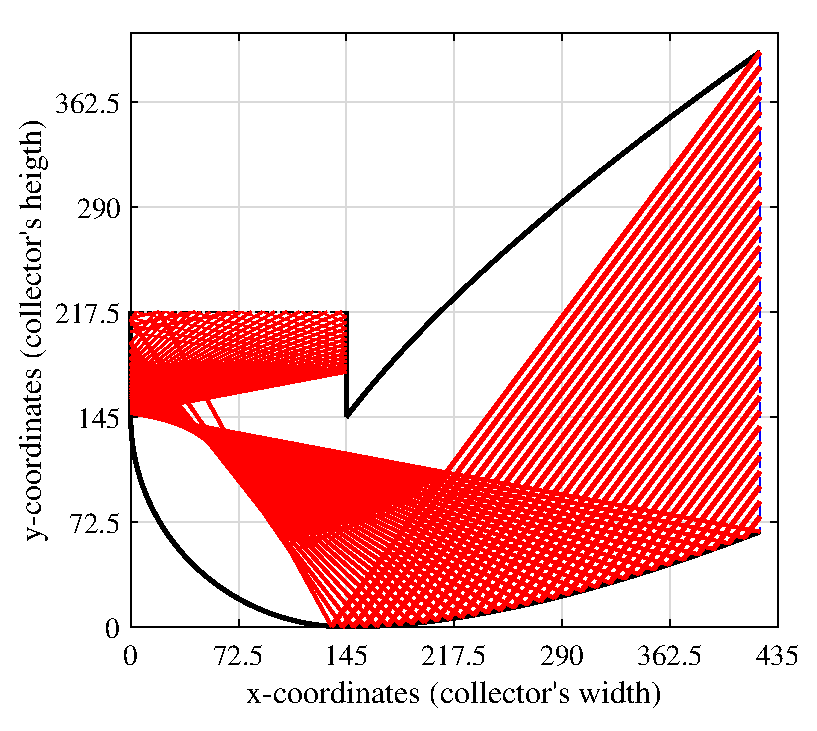
\includegraphics[scale=0.45]{figs/RT2D-hts72.eps}
		\subcaption{Ray tracing diagram (cross-section).}
		
	\end{minipage}
	\begin{minipage}{0.48\columnwidth}
		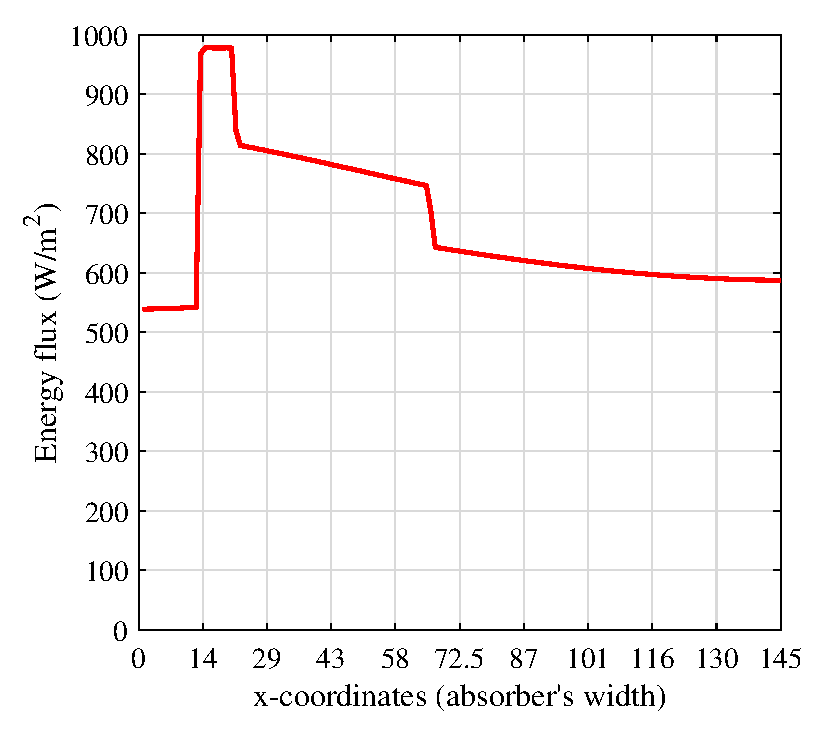
\includegraphics[scale=0.45]{figs/Energy2D-hts72.eps}
		%\\[-9mm]
		\subcaption{Energy flux distribution (cross-section).}
	\end{minipage}
	\\[3mm]
	\begin{minipage}{1.0\columnwidth}
		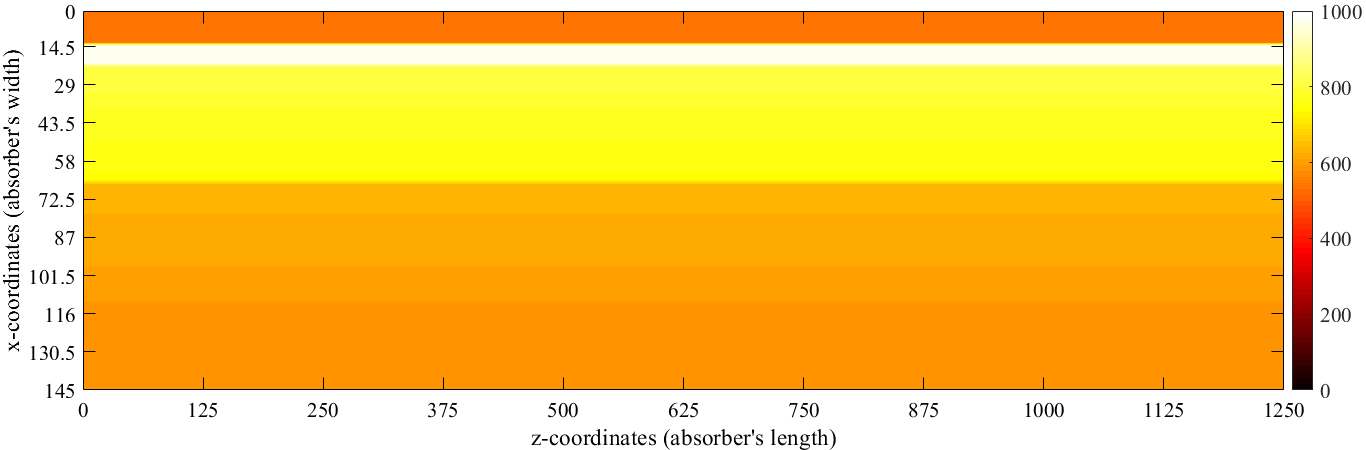
\includegraphics[scale=0.40]{figs/Energy3D-hts72.png}
		\subcaption{Energy flux distribution over the absorber surface (top view).}
	\end{minipage}
	
	\caption{Ray tracing diagram in 2D and energy flux distribution over the absorber width with tertiary section height of 72.5 mm.}
	\label{Tertiary-hts72}
\end{figure}

\newpage
From Figure \ref{Tertiary-hts145}, illustrates a scenario where the energy flux is more evenly distributed across the surface of the absorber. The maximum energy flux observed is 740 W/m$^2$ which spans across half of the absorber width. This broader distribution of energy is advantageous for improving the uniformity of heat transfer across the absorber. While the tertiary section contributes to this more balanced energy dispersion, it also leads to higher reflection losses. Despite this trade-off, the cavity height was set to be 0.145 m.

\begin{figure}[ht!]
	\begin{minipage}{0.48\columnwidth}
		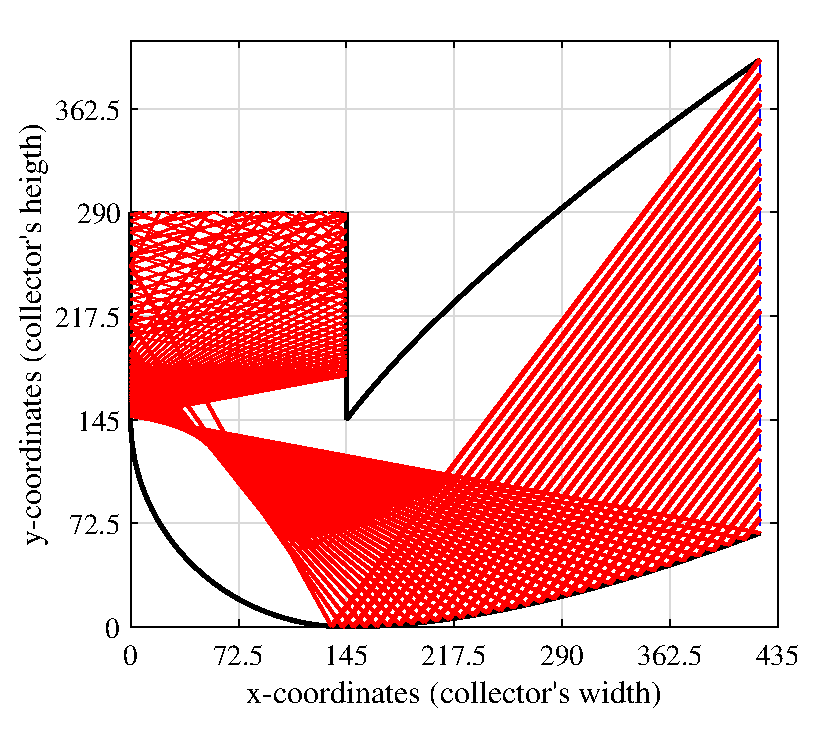
\includegraphics[scale=0.45]{figs/RT2D-hts145.eps}
		\subcaption{Ray tracing diagram (cross-section).}
		
	\end{minipage}
	\begin{minipage}{0.48\columnwidth}
		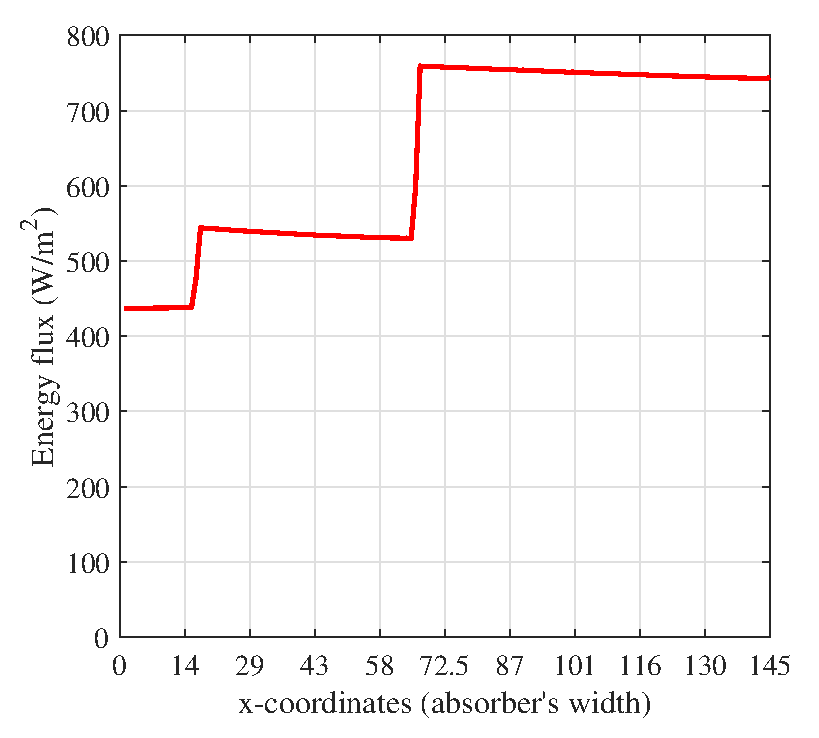
\includegraphics[scale=0.45]{figs/Energy2D-hts145.eps}
		%\\[-9mm]
		\subcaption{Energy flux distribution (cross-section).}
	\end{minipage}
	\\[3mm]
	\begin{minipage}{1.0\columnwidth}
		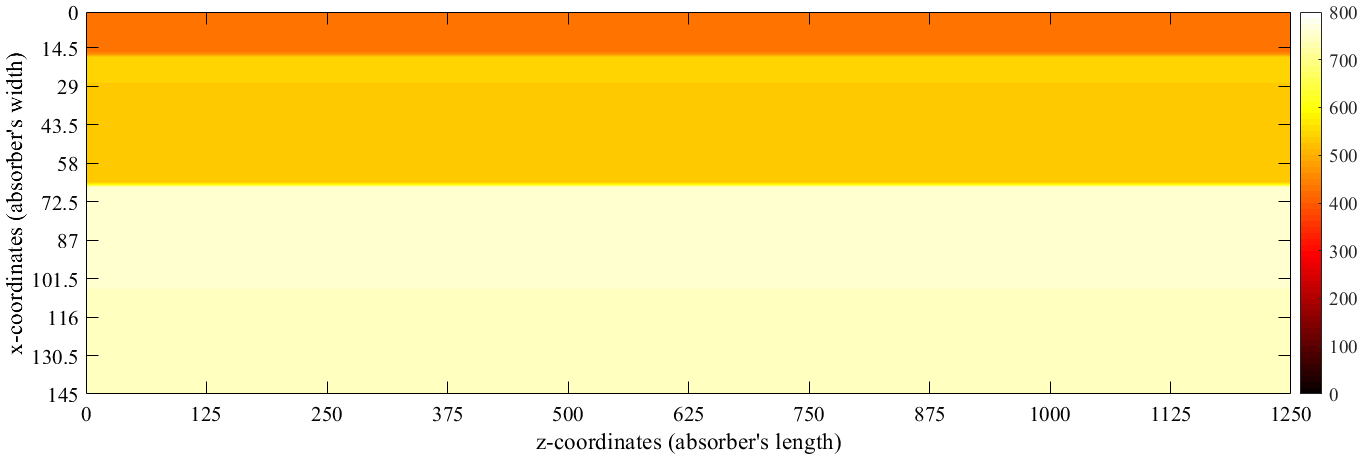
\includegraphics[scale=0.40]{figs/Energy3D-hts145.png}
		\subcaption{Energy flux distribution over the absorber surface (top view).}
	\end{minipage}
	
	\caption{Ray tracing diagram in 2D and energy flux distribution over the absorber width with tertiary section height of 145 mm.}
	\label{Tertiary-hts145}
\end{figure}

\subsection{Optical efficiency profile}

After the optical analysis, the concentrator's design was defined, as shown in Figure \ref{collector3p} and the main geometric parameters are summarised in Table \ref{optics_parameters}. The glazing inclination has been set at $\beta$ = 62$^{\circ}$ for practical reasons related to its width. 

\Figure[scale=0.70,placement=!ht,label={collector3p},caption={Cross section of the collector's final design.},frame]{figs/collector3p.eps}

\begin{table}[!ht]
	\caption{Geometric parameters of the concentrator to be fabricated.}
	\centering
	\begin{tabular}{p{1.75cm}p{4.5cm}p{2.0cm}}
		\hline \\[-10pt]
		Symbol & Geometric parameter & Value \\ [2pt]
		\hline \\[-12pt]
		$\rm{L_{col}}$ & Concentrator length & 1.25 m \\ [2pt]
		
		$\rm{H_{col}}$ & Concentrator height & 0.40 m \\ [2pt]
		
		$\rm{W_{col}}$ & Concentrator depth & 0.43 m \\ [2pt]
		
		$\rm{W_{abs}}$ & Absorber width & 0.145 m \\ [2pt]
		
		$\rm{A_{abs}}$ & Absorber area & 0.18 m$^2$ \\ [2pt]
		
		$\rm{W_{glaz}}$ & Glazing width & 0.27 m \\ [2pt]
		
		$\rm{A_{glaz}}$ & Glazing area & 0.34 m$^2$ \\ [2pt]
		
		$\beta$ & Glazing inclination & 62$^{\circ}$ \\ [2pt]
		
		$\rm{W_{apt}}$ & Aperture width & 0.33 m \\ [2pt]
		
		$\rm{A_{apt}}$ & Aperture area & 0.41 m$^2$ \\ [2pt]
		
		$\rm{H_{\!_{TS}}}$ & Cavity height & 0.145 m \\ [2pt]
		
		$\rm{CR}$ & Concentration ratio & 2.28 \\ [2pt]
		
		$\rm{A_{ref}}$ & Reflector area & 2 m$^2$ \\
		
		\hline 
	\end{tabular}
	\label{optics_parameters}
\end{table}

\newpage
Figure \ref{opt-eff-time} shows the optical profile as a function of daytime and date during the summer. The efficiency peaks between 12:00 and 14:00 during midday, as indicated by the red regions corresponding to the highest values (around 0.69). This period aligns with the solar noon, where solar altitude angle is highest, and the collector operates at maximum  optical performance. In contrast, the blue areas show that the optical efficiency diminishes in the early morning (09:00 -- 10:00) and late afternoon (16:00 -- 17:00). These lower values are likely due to reduced solar angles and optical losses due to higher reflections. Seasonal variations are also evident, with the highest efficiency observed near the summer solstice (21/06). During this time, the longer daylight hours and higher solar angles can contribute to more consistent and elevated optical efficiency throughout the day. As the dates progress toward the autumn equinox (21/09), there is a noticeable decline in efficiency, reflected by an expansion of the lower-efficiency regions (blue and green zones). This decline can be attributed to shorter daylight hours and lower solar angles as the season transitions, which increase optical losses and reduce the system's overall performance. The average optical efficiency for direct radiation of this collector is 0.67. To determine the energy an airflow absorbs, conducting experimental studies or using a reliable energy balance calculation is essential.

\Figure[scale=0.62,placement=!ht,label={opt-eff-time},caption={Optical efficiency profile throughout the whole period of operation.}]{figs/opt-eff-time.eps}

\section{Chapter Summary}

% The selection of an air heater concentrator with the absorber horizontally facing downwards aims to concentrate solar thermal energy inside the cavity and suppress heat losses. With the assistance of a ray tracing technique in 3D, an optical analysis has been undertaken to evaluate its optical efficiency considering factors as: glazing transmittance, truncation level, length and tertiary section height. The results show that there is a maximum value of optical efficiency for a particular parabolic reflector shape and a maximum value of glazing transmittance at different inclinations. It was also concluded that the energy distributed along the absorber area is more uniform with a tertiary section rather than without it even though the optical losses are higher. The effect of the tertiary section on the collector's performance needs to be further assessed, via thermal modelling and outdoor experiments. Finally, a solar concentrator design was proposed through optical analysis, and its 3D optical profile over time was presented at the end of the chapter. The proposed air heater concentrator is able to absorb in average 67\% of direct solar radiation during most part of the day in the period evaluated.

The chapter presented the design, development, and analysis of a solar air heating concentrator that integrates an inverted absorber with Asymmetric Compound Parabolic Concentrators (IACPC). This system was designed to enhance optical efficiency and reduce heat losses. The concentrator employs geometric configurations, including parabolic, circular, and straight reflectors, combined with a glazing cover to retain solar radiation and protect the system from environmental conditions. A tertiary section is added to improve energy distribution across the absorber, a feature that trades some optical efficiency for better heat transfer uniformity. The study uses 3D ray tracing simulations to evaluate the system's optical performance, focusing on factors such as glazing inclination, truncation levels, and reflector geometry. The results demonstrate an average optical efficiency of 67\% during the system's operating hours, highlighting its capability to harness direct solar radiation effectively. Key design optimisations include setting the concentration ratio at 2.28 and ensuring a compact structure with a length of 1.25 m and a height of 0.4 m. This makes the system suitable for practical applications, including integration into building fa\c{c}ades.


	\chapter{Experimental performance analysis}
\label{Cap:Exp}
%\vspace{-1.0cm}
%

This chapter aims to analyse the outdoor experimental performance of the solar air heater prototype fabricated using the concentrator designed in Chapter \ref{Cap:Opt}. This air heating system was fabricated and tested at Technological University Dublin, Ireland. The specific objectives are to:

\begin{itemize}
	\item Present the materials and components for fabrication;
	\item Describe the data collection procedure and equipment used;
	\item Evaluate the thermal performance of the system in an open loop configuration.
\end{itemize}

\section{Materials for the prototype}
	
\subsection{Absorber surface selection}

The function of the absorber surface in solar thermal systems is to retain thermal energy from incoming solar radiation. To meet this objective, carbon fibre weave fabric has been selected as the absorbing material (Figure \ref{CFphoto}). Although it is not conventionally employed in solar air heating systems (\cite{Shams2013}), its utilisation brings two advantages: i) it has natural perforations, and ii) it reduces the system's weight -- compared to an aluminium plate of the same dimensions, the carbon fibre surface is 40\% lighter.

\Figure[scale=0.3,placement=!ht,label={CFphoto},caption={Carbon fibre weave fabric (\cite{EasyComposites2017}).}]{figs/CFphoto.PNG}

\newpage
Carbon fibre weave's physical properties are presented in Table \ref{carbonfiber}. Absorptivity data were reported by \citet{Wu2012}, whereas thermal conductivity and specific heat were obtained from the material supplier Easy Composites (\cite{EasyComposites2017}). Despite being a modest thermal conductor, \citet{Gawlik2005} reported that this factor poorly influences the thermal efficiency of an air heating system with a perforated absorber.

\begin{table}[!ht]
	\caption{Carbon fibre weave properties.}
	\centering
	\begin{tabular}{p{5cm}p{4cm}}
		\hline \\[-12pt] 
		Property & Value \\ 
		\hline \\[-12pt] 
		Thickness & 0.30 mm \\ [3pt]
		Density & 1790 kg/m$^3$ \\ [3pt]
		Thermal Conductivity & 10.42 W/(m K) \\ [3pt]
		Specific Heat & 795 J/(kg K) \\ [3pt]
		Absorptivity & 0.85 \\ [1pt]
		\hline 
	\end{tabular} 
	\label{carbonfiber}
\end{table}

The carbon fibre weave fabric is made of multi-filament yarns, and the type of weave is considered according to the application (\cite{Tourlonias2016}). The area between the woven yarns are the perforations through which the flowing air passes. This porosity was calculated from data from morphology images (Figure \ref{CFmag}) by \citet{Shams2013}. The average perforation area and porosity values are 0.147 mm$^2$ and 4.2\%, respectively, and will be input as parameters in the thermal modelling depicted in \mbox{Chapter \ref{Cap:Thermal}}. The cost of this carbon fibre weave fabric was 24 \euro/${\rm m^2}$.

\Figure[scale=0.65,placement=!ht,label={CFmag},caption={Morphology image of carbon fibre sample taken at magnification of 15x.}]{figs/CFmag}

Epoxy laminating resin was applied to the corners of the surface to assemble the carbon fibre fabric onto the prototype. This was done to prevent splitting in the weave and ensure the surface remained stretched. The corners were then secured to a thin wooden frame with specific absorber dimensions (0.145 m x 1.25 m).

\subsection{Glazing cover selection}

A glazing material that enhances light transmission and avoids optical losses is needed. For the task, the selected glazing material for this system is a 4-mm thick tempered clear glass slab. This tempered property makes the glass safer and more durable than ordinary glass. It withstands 5 times more impact before shattering. If shattered, the fragments pose a reduced danger to the user, making it an attractive product for use in both commercial and domestic applications (\cite{FirstGlass2016}). The glass properties, such as absorptivity and transmittance, are shown in Table \ref{glass_tempered}. From the collector's design, the glazing dimensions are \mbox{0.27 m x 1.25 m}. The cost of the glass was 70 \euro/${\rm m^2}$.

\begin{table}[!ht]
	\caption{Glazing cover properties.}
	\centering
	\begin{tabular}{p{5cm}p{4cm}}
		\hline \\[-12pt] 
		Property & Value \\ 
		\hline \\[-12pt] 
		Thickness & 4 mm \\ [3pt]
		Density & 2500 kg/m$^3$ \\ [3pt]
		Absorptivity\footnotemark[1] & 0.02 \\ [3pt]
		Transmittance\footnotemark[1] & 0.90 \\ [3pt]
		Specific Heat & 880 J/(kg.K)  \\ [1pt]
		\hline 
	\end{tabular} 
	\label{glass_tempered}
\end{table}

\footnotetext[1]{Values at near normal incident light}

\subsection{Reflector surface selection}

The reflective material employed is \textit{MiroSun} from the German company Alanod, the only product used for solar applications. This reflective aluminium sheet is manufactured using a continuous physical vapour deposition (PVD) process applied for a super reflective layer to coil anodised material. Afterwards, the surface is protected by a nano-composite in a coil-coating process. Table \ref{reflector_M} shows the optical and physical properties of this material. From the concentrator's design, the total area of the reflector sheet used was 1.25 m x 1.20 m. The cost of the Alanod reflector was 50 \euro/${\rm m^2}$.

\begin{table}[!ht]
	\caption{\textit{MiroSun} reflector properties (\cite{Alanod2016}).}
	\centering
	\begin{tabular}{p{5cm}p{4cm}}
		\hline \\[-12pt] 
		Property & Value \\ 
		\hline \\[-12pt] 
		%Front Side Layer & PVD improved \\ [3pt]
		%Reverse Side Layer & Anodised \\ [3pt]
		Thickness & 0.5 mm \\ [3pt]
		Density & 2700 kg/m$^3$ \\ [3pt]
		%Max. Width & 1.25 m \\ [3pt]
		Total Reflectivity & 0.95 \\ [1pt]
		\hline 
	\end{tabular} 
	\label{reflector_M}
\end{table}

\subsection{Prototype's structure}

The materials used to fabricate the prototype's structure are listed as follows:

\begin{itemize}
	\item 0.7 m$^2$ of a 2-mm thick aluminium sheet to form the ends;
	\item 8 aluminium bars of 1.25 m in length to support and keep the reflectors in the desired position;
	\item 0.45 m$^2$ of 1-cm thick timber to form a cavity above the absorber surface in order to reduce heat losses;
	\item two 2.5-in diameter aluminium pipes of 10 cm in length for the airflow inlet and outlet;
	\item 1.8 m$^2$ of a 0.6-mm thick aluminium sheet to box the whole structure.
	
\end{itemize}

Figure \ref{Ass11} shows photographs of the assembled structure. The space between the reflectors and the outer aluminium sheet was filled with fibre glass wool to provide thermal insulation. The structure was wrapped with polyurethane foam board and sealed with waterproof tape.

\begin{figure}[ht!]
	\begin{minipage}{0.49\columnwidth}
		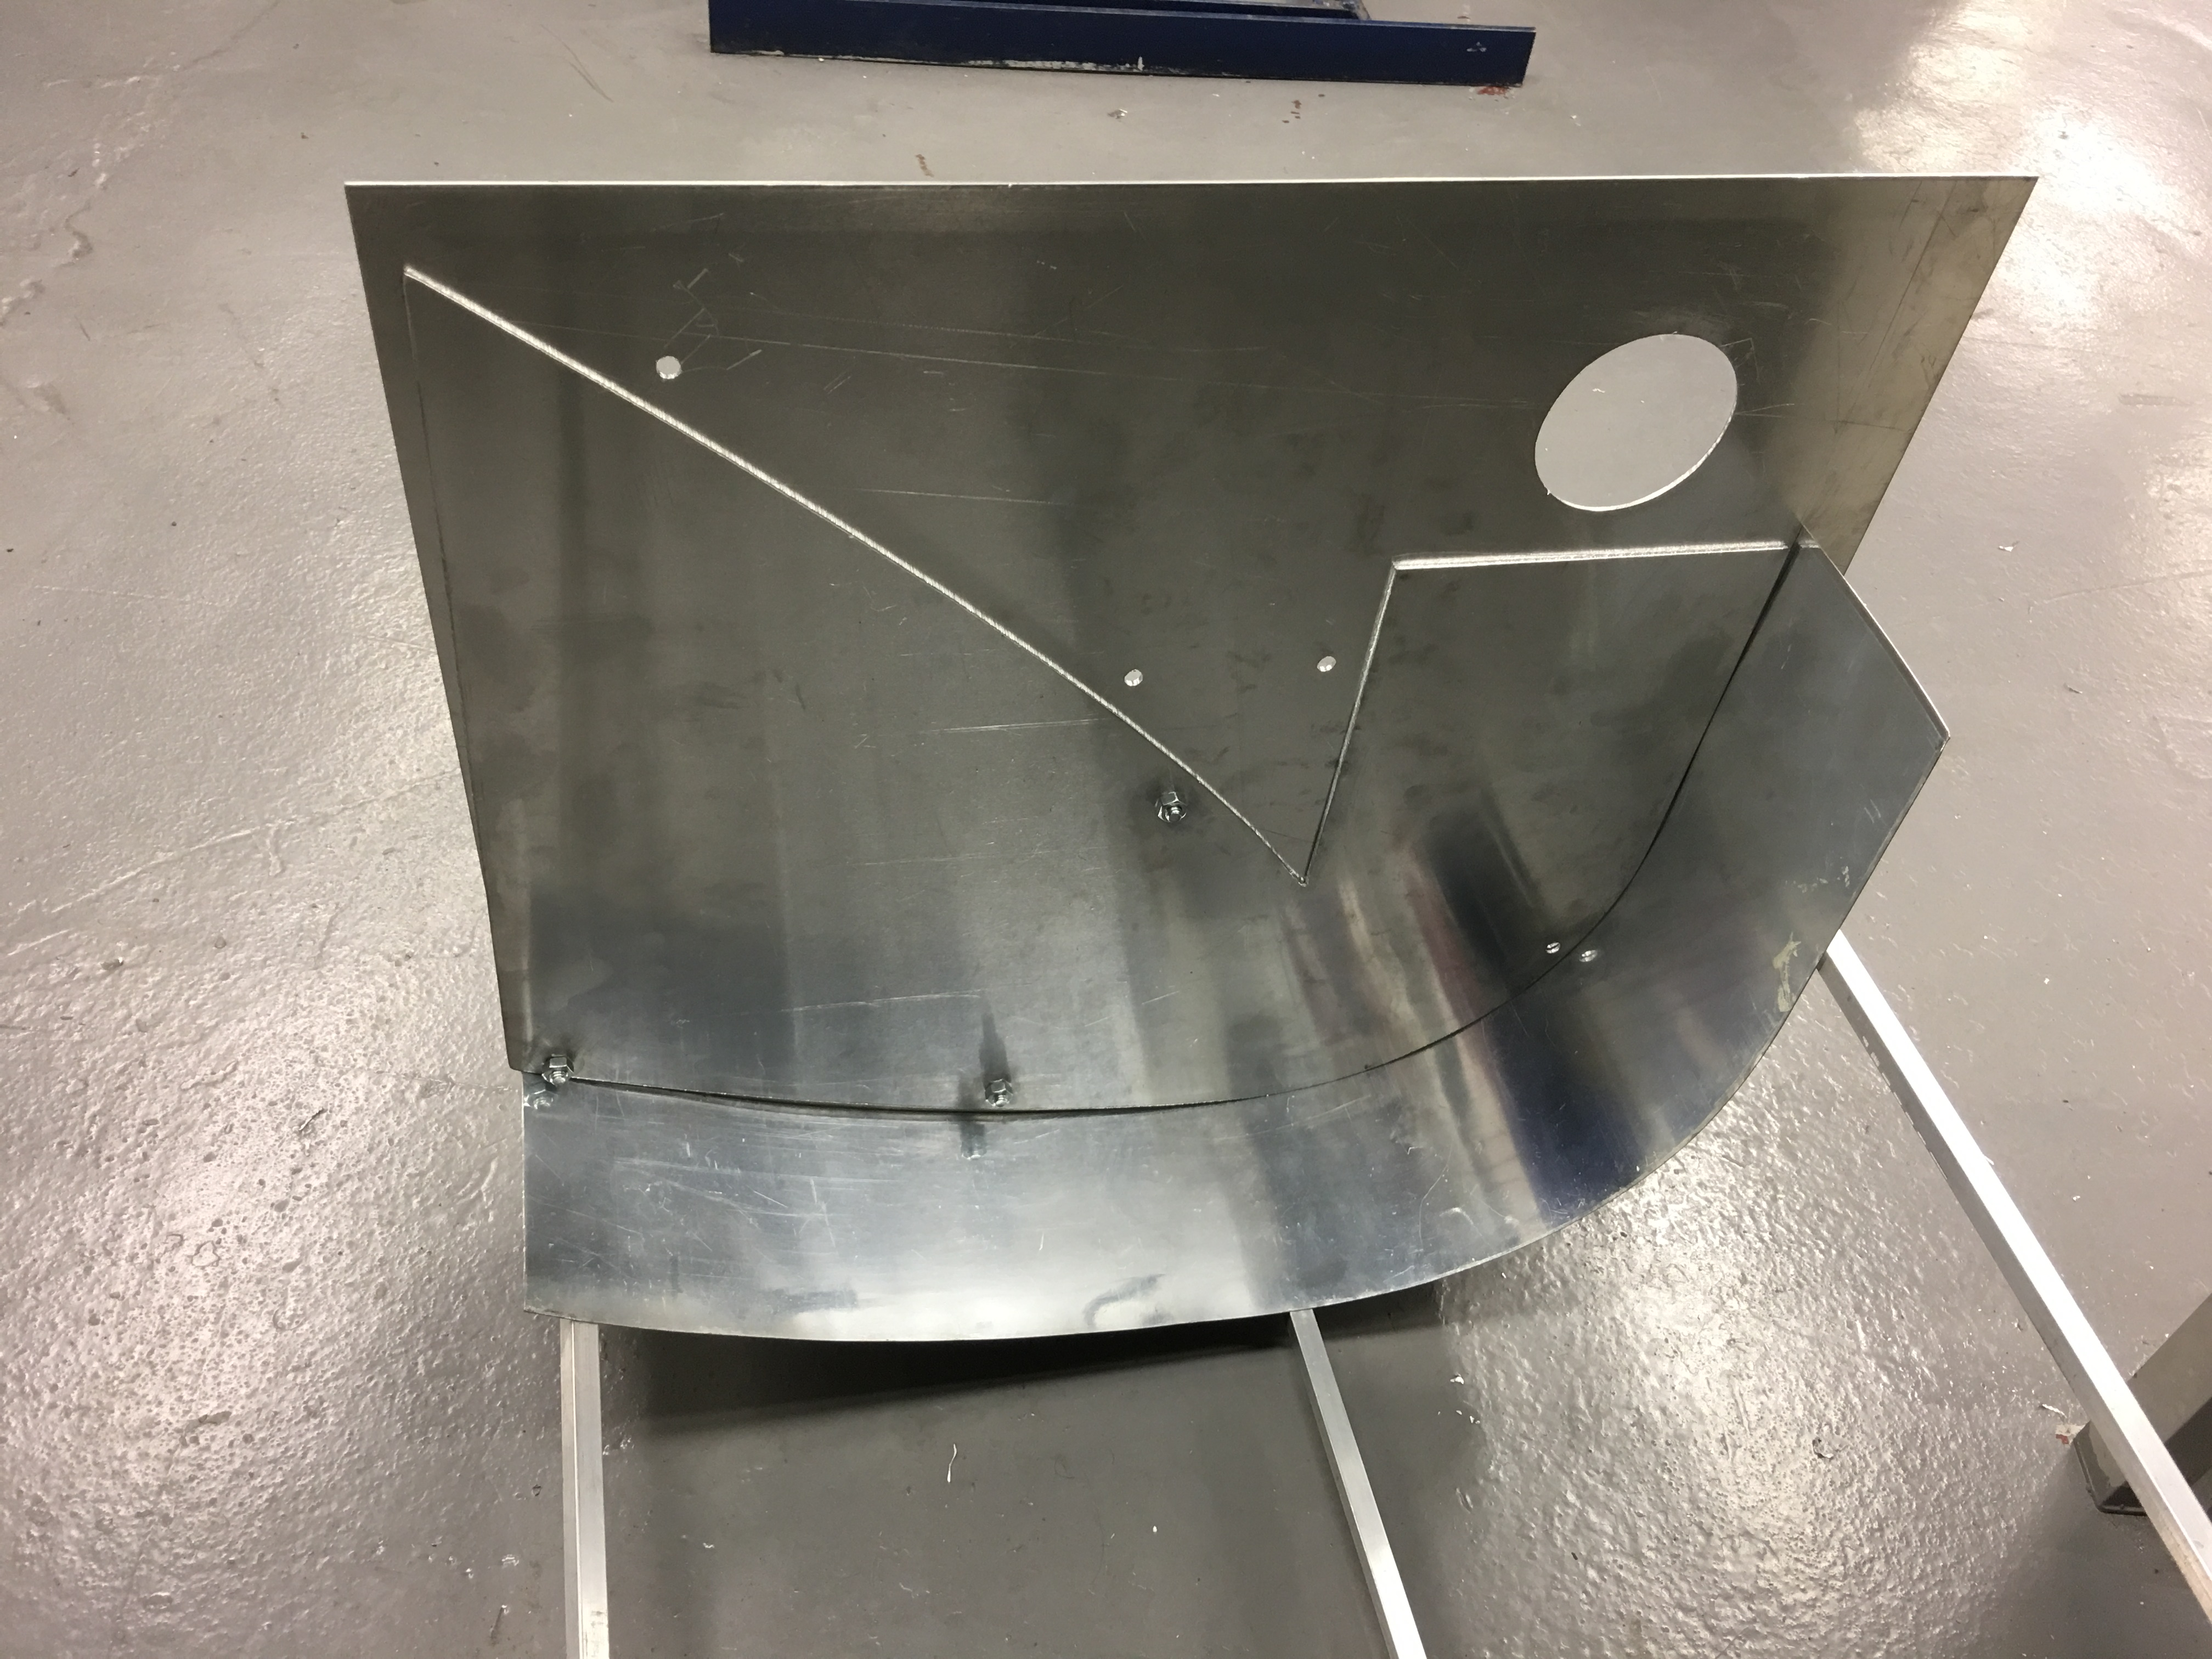
\includegraphics[width=0.95\columnwidth,height=5cm]{figs/Ass1.jpg}
		\subcaption{One end assembled.}
		
		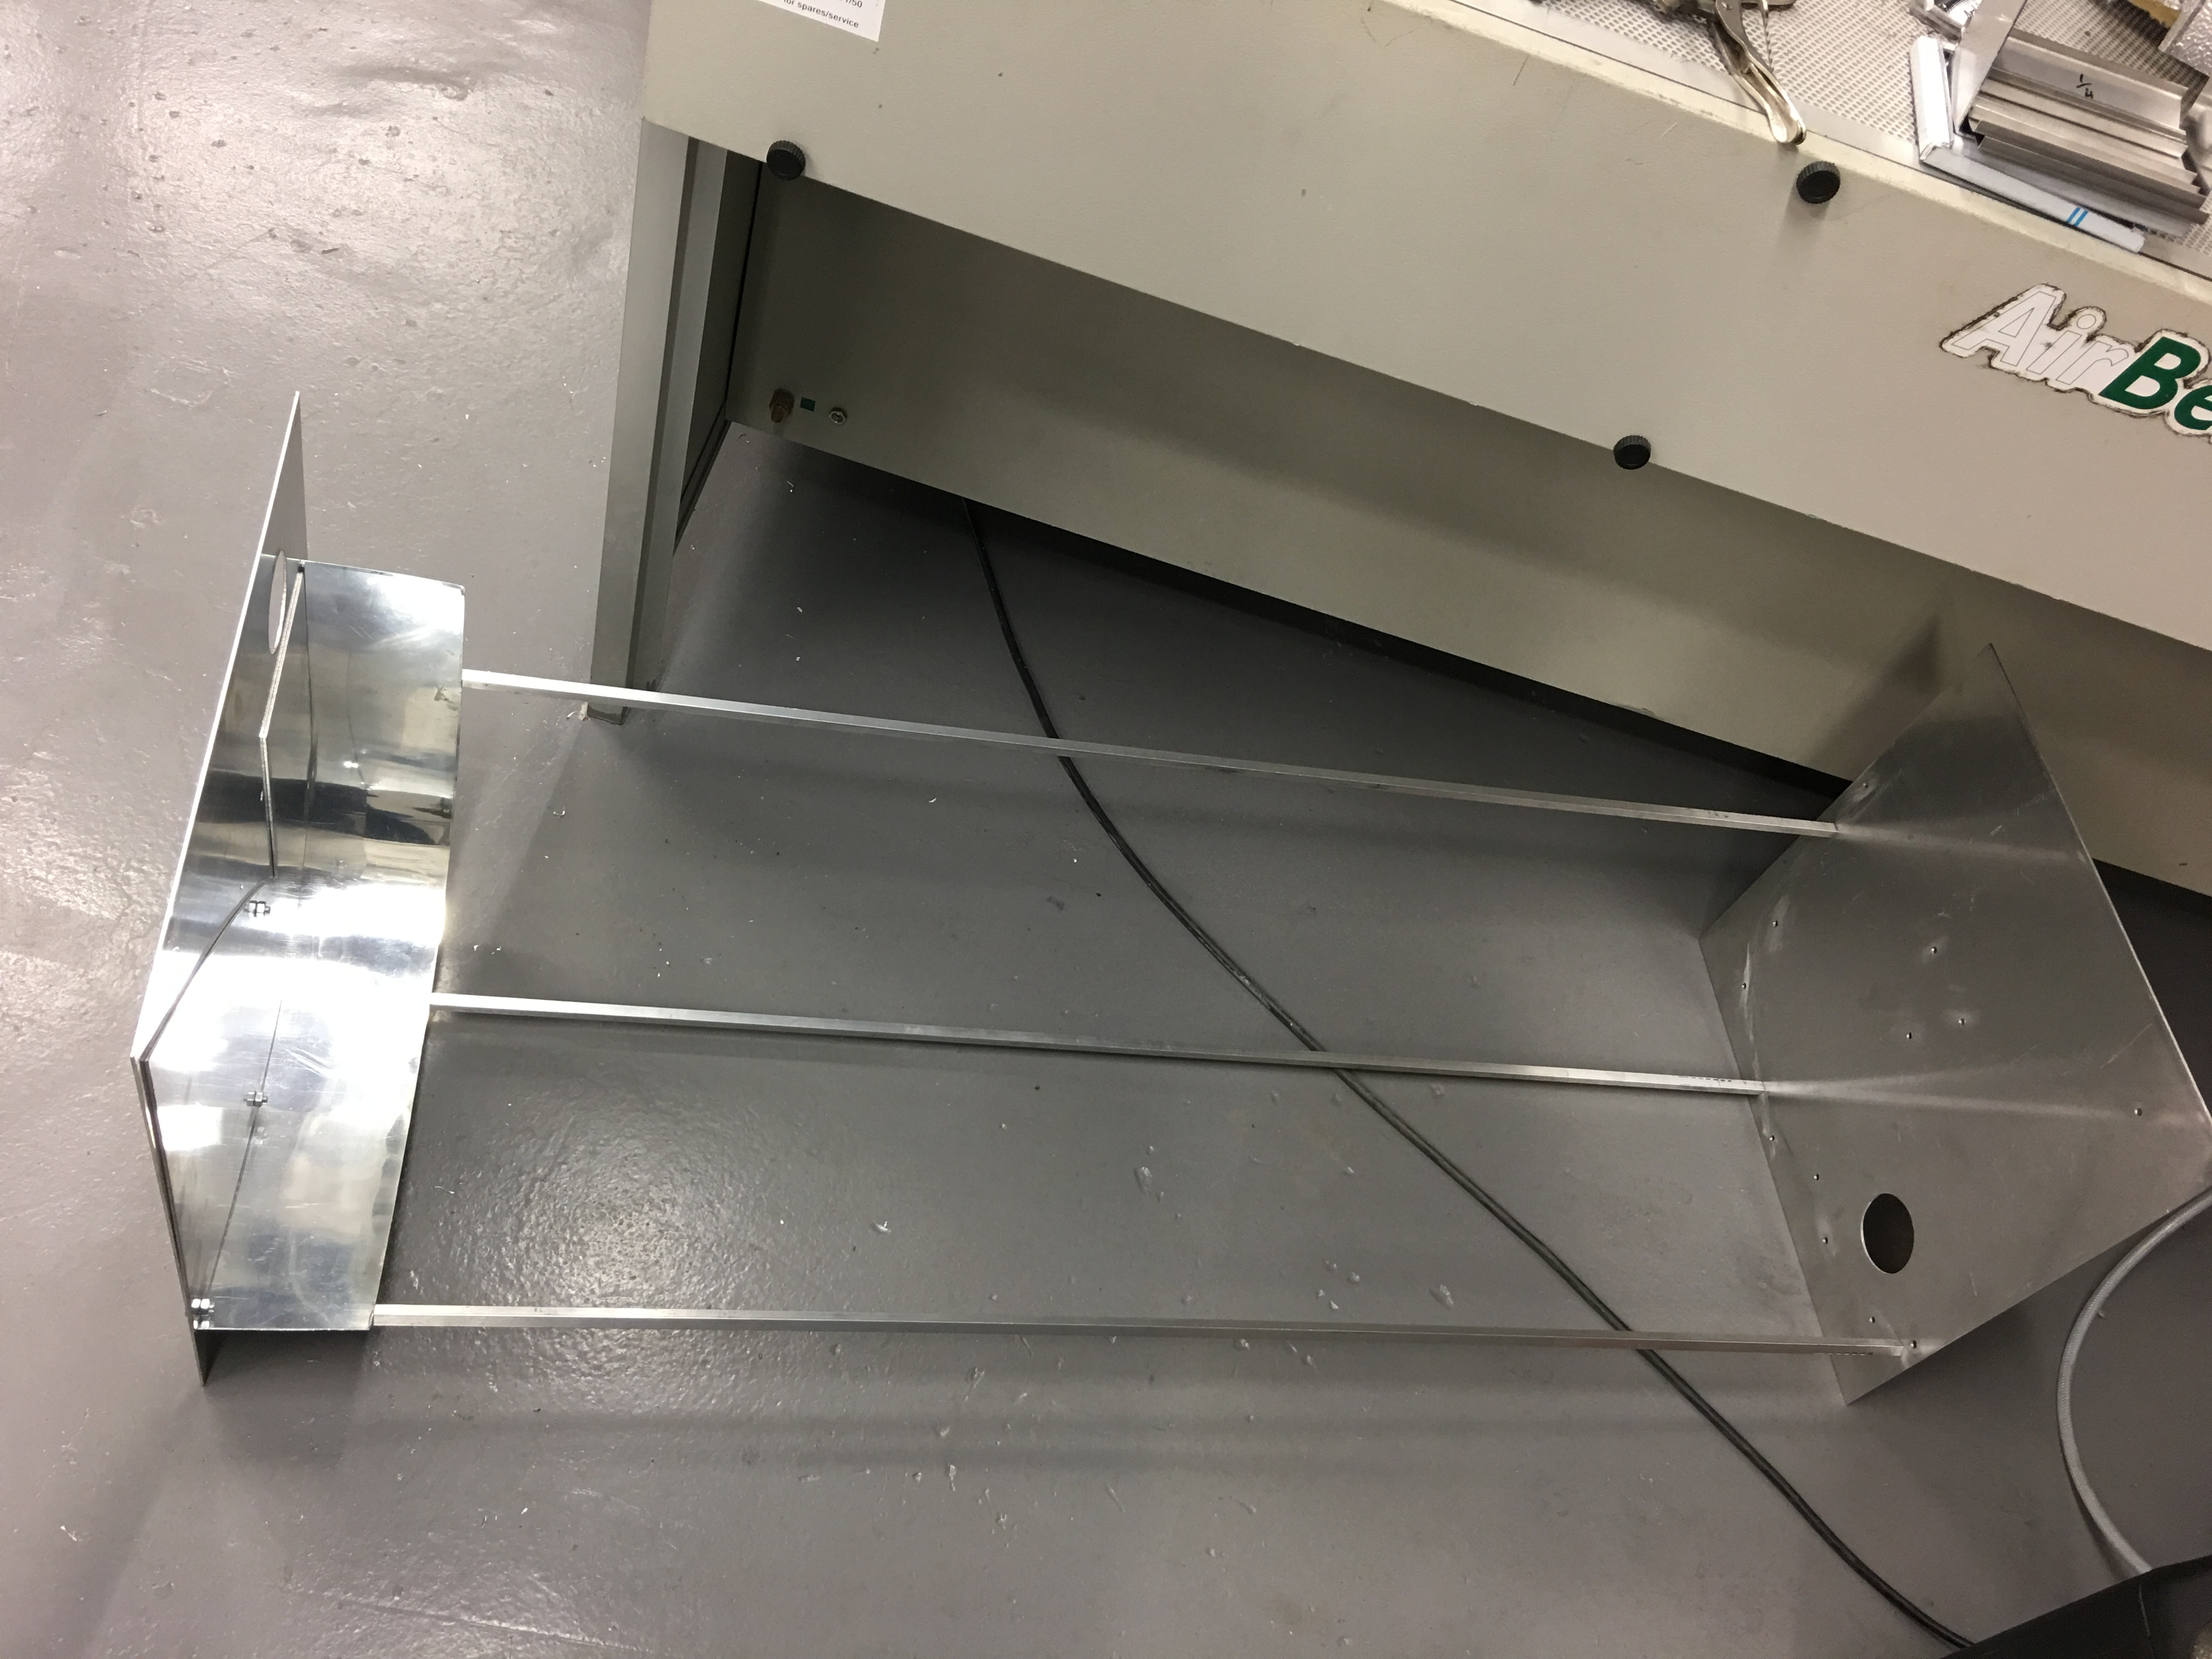
\includegraphics[width=0.95\columnwidth,height=5cm]{figs/Ass2.jpg}
		\subcaption{Two ends and aluminium bars assembled.}
	\end{minipage}
	\begin{minipage}{0.49\columnwidth}
		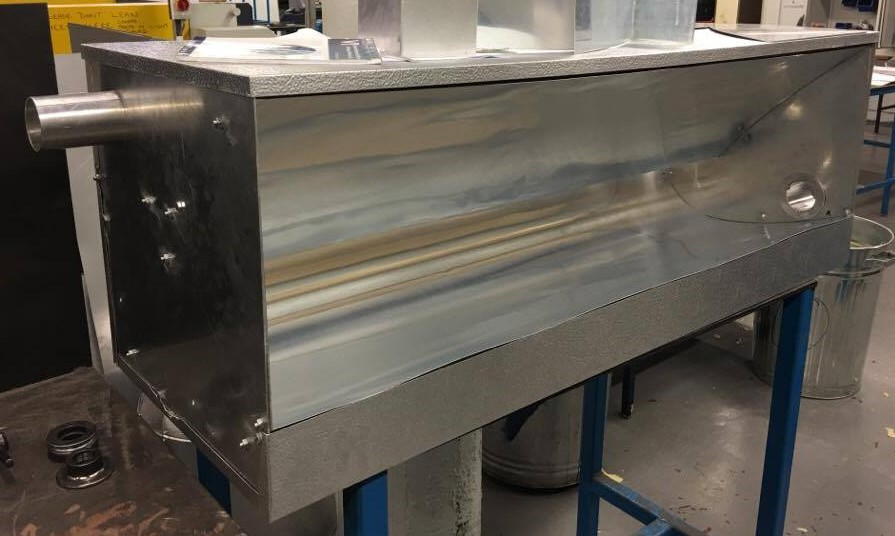
\includegraphics[width=0.95\columnwidth,height=5cm]{figs/Ass4.jpg}
		\subcaption{Closed structure.}
		
		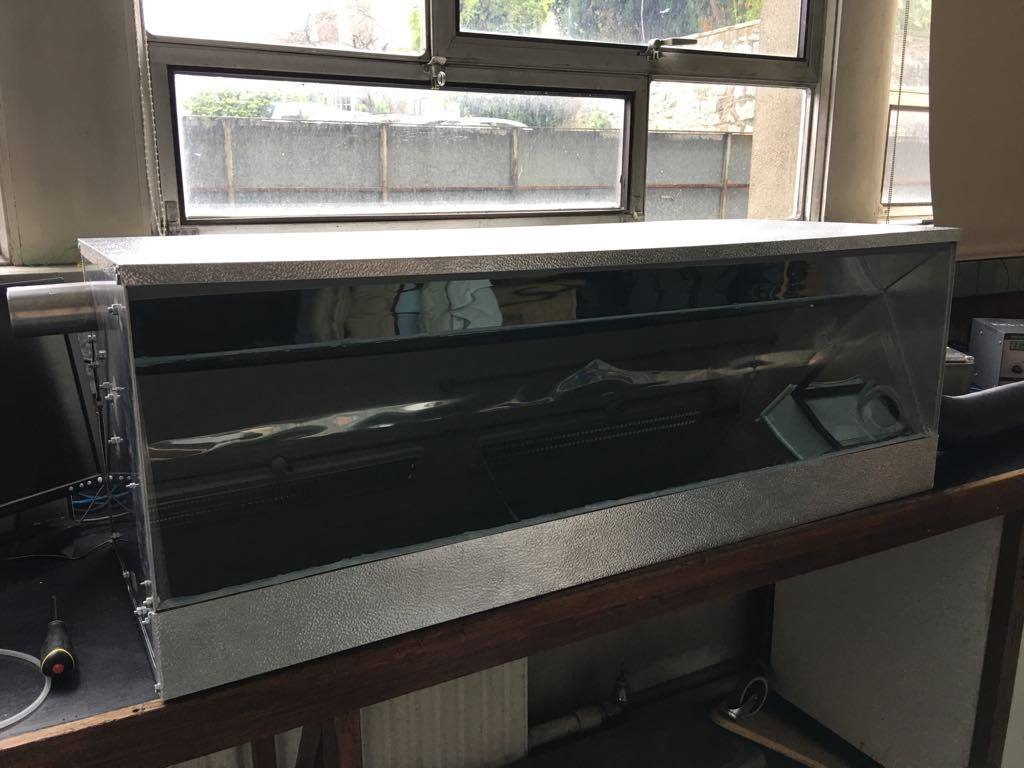
\includegraphics[width=0.95\columnwidth,height=5cm]{figs/Ass3.jpg}
		\subcaption{Closed structure with the glass.}
		
	\end{minipage}
	\caption{Parts of the prototype's structure and assembled}
	\label{Ass11}
\end{figure}

%\Figure[scale=0.45,placement=!ht,label={Structure1},caption={Aluminium structure of the solar air heater.}]{figs/Structure1.png}

\section{Instrumentation of the experimental unit}

Temperatures were measured at the inlet and outlet of air, absorber and glazing surfaces using type T (Cu-CuNi) PTFE insulated twist fine wire thermocouple sensors with an accuracy of $\pm$0.5 $^{\rm{o}}$C. Figures \ref{TC_abs} and \ref{TC_glaz} indicate the position of each thermocouple on the absorber and glazing surfaces, respectively. 18 thermocouples were used in total. As a matter of orientation, in both figures, the side where the thermocouple 1 is placed is the closest to the outlet.

\Figure[scale=0.50,placement=!ht,label={TC_abs},caption={Positions of the 12 thermocouples numbered from 1 to 12 placed on the absorber surface (dimensions in mm).}]{figs/absorber_thermocouple.PNG}

\Figure[scale=0.40,placement=!ht,label={TC_glaz},caption={Position of the three thermocouples numbered from 1 to 3 placed on the glazing surface (dimensions in mm).}]{figs/glass_thermocouple.PNG}

These temperature measurements were recorded at 1-minute intervals with a DL2e data logger connected directly to a computer, where the temperature data were downloaded via a USB port (\cite{Devices2018}). All thermocouples were labelled, inserted in a plug and connected to the data logger.

\newpage
The airflow was provided by a 12-W fan, where the rate was varied by a voltage adaptor with five different voltage inputs. The air velocity at the air outlet ($\rm{v_{in}}$, in m/s) was measured using a Testo 425 hot wire anemometer. These velocity levels were converted to airflow values using Eq. (\ref{Gpitot}).

%\begin{equation}
%\mathrm{{v_{out}} = \sqrt {\frac{{2{\mathrm{P_{out}}}}}{{{\mathrm{d_{air}}}}}}}
%\label{Vpitot}
%\end{equation}

\vspace{-0.75cm}
\begin{equation}
\mathrm{{G_{air}} = \frac{{{v_{in}}{A_{out}}{d_{air}}}}{{{A_{abs}}}}}
\label{Gpitot}
\end{equation}

\noindent where $\rm{A_{out}}$ is the cross-section area of the outlet pipe (m$^2$), $\rm{d_{air}}$ is the air density (kg/m$^3$) and  $\rm{G_{air}}$ is the mass airflow rate per absorber area (kg/(s.m$^{{\rm{2}}}$)).

The measured variables are subjected to systematic uncertainties due to instrumentation errors. It is thus necessary to calculate the standard uncertainty of each variable measured for the experimental work. Those measurements are temperature, air velocity and solar radiation. The accuracy of each instrument, taken from the manufacturer data is shown in Table \ref{uncertainty}.   

\begin{table}[!ht]
	\caption{Measurements and standard uncertainty.}
	\centering
	\begin{tabular}{p{3.0cm}p{3.5cm}p{3.5cm}}
		\hline \\[-10pt] 
		\rule[-1ex]{0pt}{2.5ex} Measurement & Accuracy & Uncertainty \\ [3pt]
		\hline \\[-10pt]
		\rule[-1ex]{0pt}{2.5ex} Temperature & ${\rm \pm0.55 ^{\rm o}C \pm0.3 ^{\rm o}C}$ & 0.36 $^{\rm o}$C \\ [5pt]
		\rule[-1ex]{0pt}{2.5ex} Air velocity &  $\pm$(0.03 + 5\% of ${\rm v_{in})}$ & 0.0173 + 0.0289${\rm v_{in}}$ \\ [5pt] 
		%\rule[-1ex]{0pt}{2.5ex}  & 0.070 & 650 \\ [5pt]
		%\rule[-1ex]{0pt}{2.5ex} 8.70 & 0.090 & 820 \\ [5pt]
		\rule[-1ex]{0pt}{2.5ex} Solar radiation & -- & 1\% of ${\rm I_{\!_T}}$ \\ [2pt]
		\hline 
	\end{tabular}
	\label{uncertainty}
	
\end{table}


\newpage
Table \ref{GxV} shows the air velocity and airflow rate values as a function of the voltage input input ($\rm{V_a}$) and a category corresponding to each level. Systematic uncertainties were also calculated for the airflow rate (${\rm u_g}$).

\begin{table}[!ht]
	\caption{Mass and volumetric flow rates calculated at each voltage input.}
	\centering
	\begin{tabular}{p{2.1cm}p{1.8cm}p{2.4cm}p{2.2cm}p{1.8cm}}
		\hline \\[-10pt] 
		\rule[-1ex]{0pt}{2.5ex} Voltage (V) & ${\rm v_{in}}$ (m/s) & $\rm{G_{air}}$ (kg/m$^2$.s) & ${\rm u_{g}}$ (kg/m$^2$.s)  & Code \\ [3pt]
		\hline \\[-10pt]
		\rule[-1ex]{0pt}{2.5ex} 4.92 & 1.83 & 0.038 & 0.0021 & Low\\ [5pt]
		\rule[-1ex]{0pt}{2.5ex} 5.82 & 2.59 & 0.054 & 0.0030 & Low-med \\ [5pt] 
		\rule[-1ex]{0pt}{2.5ex} 7.20 & 3.43 & 0.071 & 0.0039 & Medium \\ [5pt]
		\rule[-1ex]{0pt}{2.5ex} 8.70 & 4.30 & 0.089 & 0.0048 & Med-high  \\ [5pt]
		\rule[-1ex]{0pt}{2.5ex} 11.30 & 5.50 & 0.114 & 0.0060 & High \\ [2pt]
		\hline 
	\end{tabular} 
	\label{GxV}
\end{table}

%Hence, a 2$^{\rm{nd}}$ degree polynomial was fit from the previous data, as shown in \mbox{Eq. (\ref{Gfit}):} 

%\begin{equation}
%\mathrm{{G_{air}} =  - 6.3 \cdot {10^{ - 4}}V_a^2 + 0.022V_a - 0.054}
%\label{Gfit}
%\end{equation}

%The pressure drop across the prototype was calculated at each airflow level and are presented in Figure \ref{dP-Gair}.

%\Figure[scale=0.50,placement=!ht,label={dP-Gair},caption={Pressure drop for different mass airflow rates}]{figs/dP-Gair.eps}

An open-loop experimental system diagram is shown in Figure \ref{scheme_p}. A flexible duct was connected to the prototype's inlet. The fan flowed air through the duct to the collector. The power supply unit provided voltage to the fan and energy to the data logger.

\Figure[scale=0.90,placement=!ht,label={scheme_p},caption={Schematic diagram of the experimental unit.}]{figs/scheme_prototype.png}

Figure \ref{unit1} presents the prototype's front view. It was fixed to the ground to prevent it from moving due to severe wind conditions. The fan was enclosed and protected from the environment during the experiments, and the data logger was placed behind the prototype.

\Figure[scale=0.48,placement=!ht,label={unit1},caption={Open-loop outdoor prototype.}]{figs/unit3.png}

\section{Experimental results from the air heating prototype}

This section presents the experimental results from tests conducted at the five airflow rates and those without flow. The thermal performance of the prototype focused on evaluating the useful energy rate (or energy delivered), collector thermal efficiency and outlet air temperature. The useful heat rate transferred to the airflow is estimated by Eq. (\ref{usefulenergy}) (\cite{Kalogirou2004}) using temperature measurements from the inlet and outlet:

\vspace{-0.75cm}
\begin{equation}
\mathrm{{Q_u} = {G_{air}}{A_{abs}}{C_{p,air}}({T_{out}} - {T_{in}})}
\label{usefulenergy}
\end{equation}

The thermal efficiency, which is the ratio of useful heat rate to the incoming total solar radiation on the aperture, is calculated by Eq. (\ref{ThermalEf0}). The solar radiation data used in the calculations were downloaded from the Met Eireann website (\cite{MetEireann2018}). Such data were measured by a solar pyranometer placed at the horizontal.

\subsection{Experimental results at transient state}

Experimental results of measured temperatures and solar radiation were used to calculate energies and thermal efficiency hourly. One day of each level of airflow rate was taken for data treatment and discussion, from 9:00 to 17:00 in 2018. 

\subsubsection{Experimental results at zero airflow}

The equilibrium temperature that the absorber approaches when no energy is removed from the collector is known as the stagnation temperature (\cite{Rabl1985}). To verify this condition, the system's inlet and outlet were closed, and two tests were conducted on clear sky days, specifically on 2$^{\rm{nd}}$ and 3$^{\rm{rd}}$ July, as shown in Figure \ref{zero12}. The temperature profile of the absorber represents the average measurements from all 12 thermocouples placed on its surface. During both tests, peaks of maximum stagnation absorber temperatures reached 77 $^{\rm{o}}$C with an average $\rm{I_{\!_T}}$ of 830 W/m$^{\rm{2}}$ and $\rm{T_{amb}}$ of 22 $^{\rm{o}}$C occuring around 14:00 on both days.

\Figure[scale=0.70,placement=!ht,label={zero12},caption={Experimental results from 2$^{\rm{nd}}$ and 3$^{\rm{rd}}$ July at zero airflow.}]{figs/zero12.eps}

Figure \ref{thermocouples} shows the measured temperatures for each thermocouple positioned on the absorber surface in order to investigate the stagnation point. The temperatures at the left end (T10/T11/T12) are slightly higher than those at the right (T1/T2/T3). This difference can be attributed to the fact that at 14:00 on 2$^{\rm nd}$ July, the Sun's altitude and azimuth angles are 59$^{\rm o}$ and 14\textdegree. Consequently, a concentration of energy may be occurring on the left side, which explains the temperature variation. Another observation is that the energy flux was well distributed along the area, as most temperatures are near the average value.

\Figure[scale=0.40,placement=!ht,label={thermocouples},caption={Temperatures measured by the thermocouples on the absorber surface.}]{figs/thermocouples.png}

This result can be compared to the energy distribution obtained by the ray tracing algorithm used in Chapter 3 and shown in Figure \ref{case_ch4}. The analysis indicates that the left end of the absorber surface received significantly more energy compared to the right end, which is clearly reflected in the corresponding measured temperatures. In particular, the higher temperatures at the left end suggest that it is more effectively absorbing energy. Conversely, although the right end does not receive direct radiation, its temperatures are still relatively close to the average. This suggests that some level of energy redistribution or thermal conduction may be occurring. In summary, this analysis provides a means to validate the previously developed optical modelling.

\Figure[scale=0.40,placement=!ht,label={case_ch4},caption={Energy distribution on the absorber surface obtained via ray tracing, where the Sun's altitude and azimuth angles are 59$^{\rm o}$ and 14\textdegree.}]{figs/case_ch4.eps}

\newpage
\subsubsection{Experimental results with airflow}

The findings of a low airflow rate (0.038 kg/m$^2$.s) experiment are presented in Figure \ref{004}. It was conducted on 9$^{\rm{th}}$ June under clear sky conditions with the highest solar radiation values at the solar noon hour (13:00 -- 14:00), where its peak is 860 W/m$^2$. During this hour, the average outlet airflow temperature $\rm{T_{out}}$, ambient temperature $\rm{T_{amb}}$, and thermal efficiency $\eta_{\rm{th}}$ were observed to have average values of 51 $^{\rm{o}}$C, 23 $^{\rm{o}}$C, and 0.53, respectively. At around the peak of solar radiation, the maximum $\rm{T_{out}}$ was found to be 51~$^{\rm{o}}$C, resulting in an airflow temperature rise of 28 $^{\rm{o}}$C and a corresponding $\eta_{\rm{th}}$ of 0.54. The total incident solar radiation received during the test was estimated to be 20.46 MJ/m$^2$, of which a total useful energy collected $\rm{Q_{u}}$ of 7.64 MJ/m$^2$ was calculated, resulting in a daily thermal efficiency of 0.35.

\begin{figure}[!ht]
	\centering
	\begin{minipage}{0.49\textwidth}
		\centering
		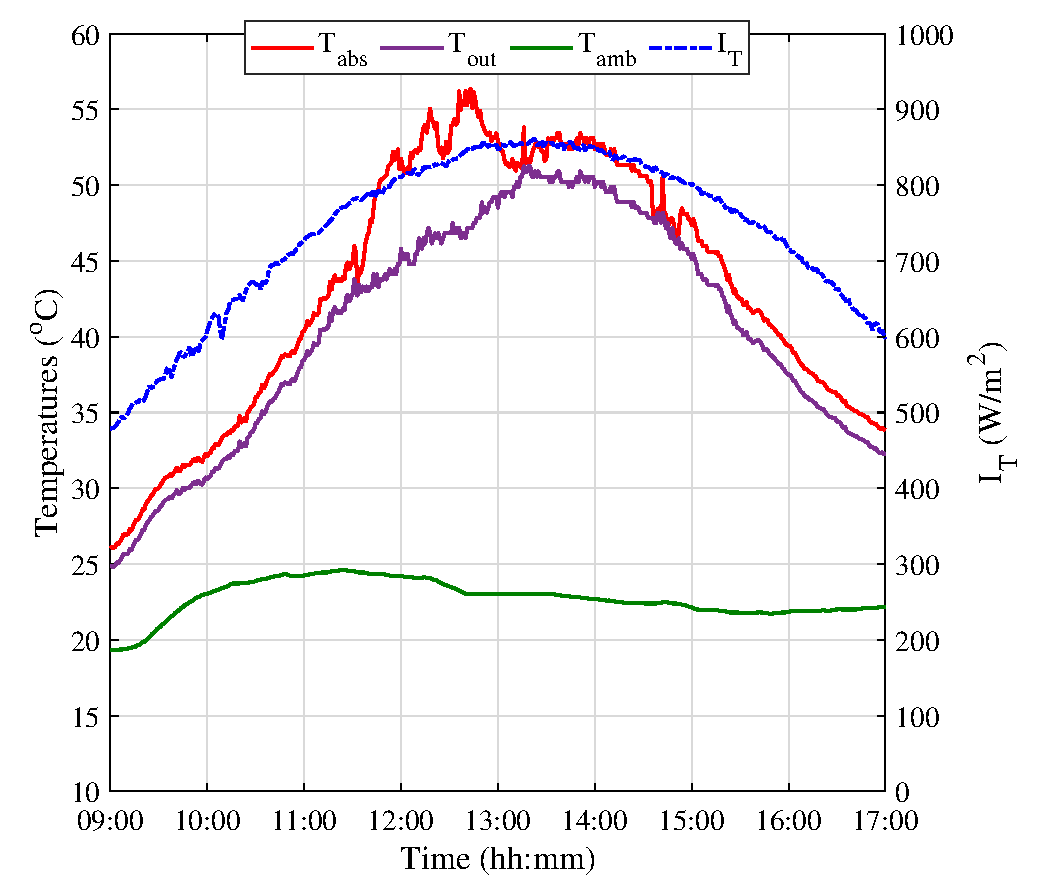
\includegraphics[width=0.98\textwidth]{figs/004-1.eps} % first figure itself
		\subcaption{Temperature results and solar data.}
	\end{minipage}\hfill
	\begin{minipage}{0.49\textwidth}
		\centering
		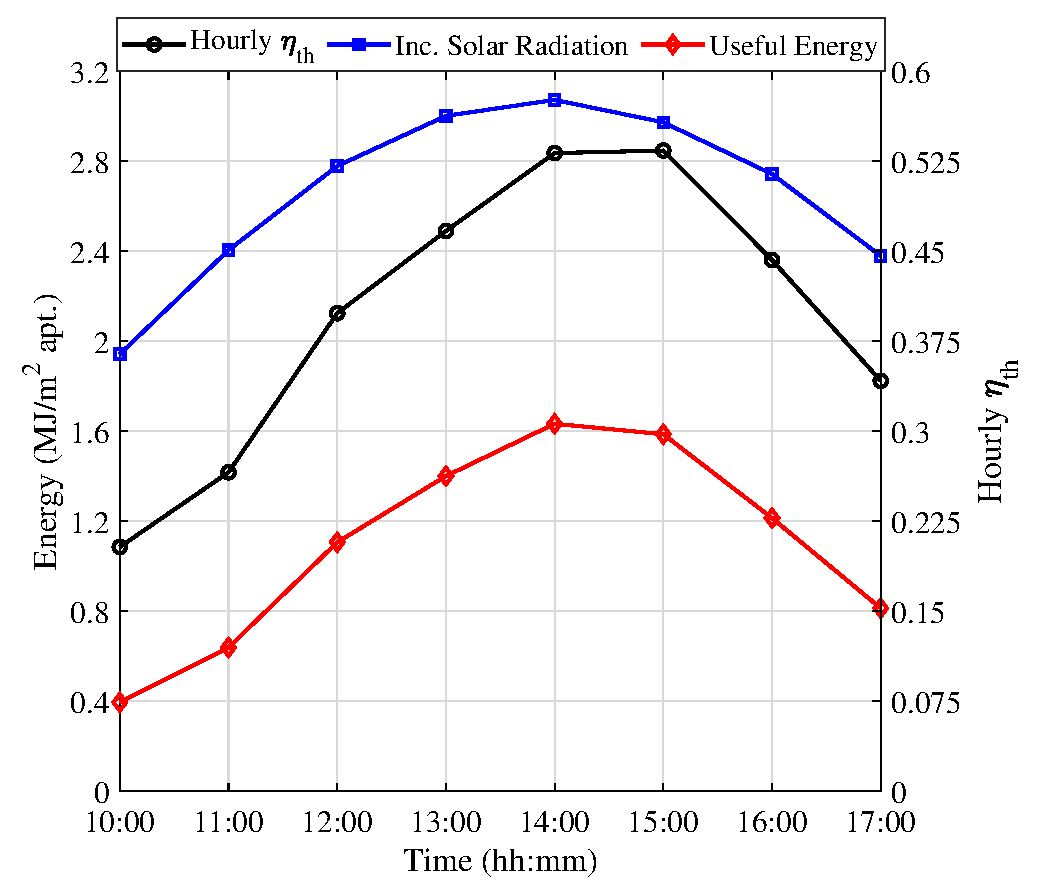
\includegraphics[width=0.98\textwidth]{figs/004-2.eps} % second figure itself
		\subcaption{Hourly performance and solar data.}
	\end{minipage}

	\caption{Experimental results from 9$^{\rm{th}}$ June at 0.038 kg/(s m$^2$).}
	\label{004}
\end{figure}

The results of an experiment conducted at a low-medium airflow rate (0.055 kg/m$^2$.s) under relatively clear sky conditions are depicted in Figure \ref{0055}. During the solar noon hour (13:00 -- 14:00), the airflow collected 1.7 MJ/m$^2$ of energy at an average outlet temperature of 43 $^{\rm{o}}$C and thermal efficiency of 55\%. The highest outlet temperature ($\rm{T_{out}}$) was recorded as 42 $^{\rm{o}}$C when the ambient temperature ($\rm{T_{amb}}$) was 20 $^{\rm{o}}$C, resulting in a maximum temperature rise of 22 $^{\rm{o}}$C. The total solar energy available was 21.29 MJ/m$^2$, while the total useful energy collected was 9.56 MJ/m$^2$. The thermal efficiency obtained for this day was 43\%.

%The highest outlet temperature ($\rm{T_{out}}$) was recorded as 43 $^{\rm{o}}$C when the ambient temperature ($\rm{T_{amb}}$) was 21 $^{\rm{o}}$C. The maximum temperature rise of the airflow was observed to be 22 $^{\rm{o}}$C, and the corresponding thermal efficiency ($\eta_{\rm{th}}$) during this period was estimated at 55\%. The total solar energy available was 21.29 MJ/m$^2$, while the total useful energy collected was 9.56 MJ/m$^2$. The thermal efficiency obtained for this day was 43\%. During the solar noon hour (13:00 -- 14:00), the airflow collected 1.7 MJ/m$^2$ of energy at an average outlet temperature of 43 $^{\rm{o}}$C.

%The experimental results of this test operating at low-med airflow (0.055 kg/m$^2$.s) are shown in Figure \ref{0055} under relatively clear sky condition. The highest $\rm{T_{out}}$ measured was 43 $^{\rm{o}}$C  when $\rm{T_{in}}$ = 23 $^{\rm{o}}$C and $\rm{T_{amb}}$ = 21 $^{\rm{o}}$C. The maximum airflow temperature rise was 20 $^{\rm{o}}$C observed between 13:00 and 14:00. The thermal efficiency ($\eta_{\rm{th}}$) on this same region was 55\%. The total solar energy available on 22$^{\rm{nd}}$ June was 21.29 MJ/m$^2$; the total useful energy collected was 9.56 MJ/m$^2$; and the thermal efficiency for this day obtained was 43\%. In the hour of solar noon (13h -- 14h), the airflow collected 1.7 MJ/m$^2$ of energy at an average $\rm{T_{out}}$ of 43 $^{\rm{o}}$C.


\begin{figure}[!ht]
	\centering
	\begin{minipage}{0.49\textwidth}
		\centering
		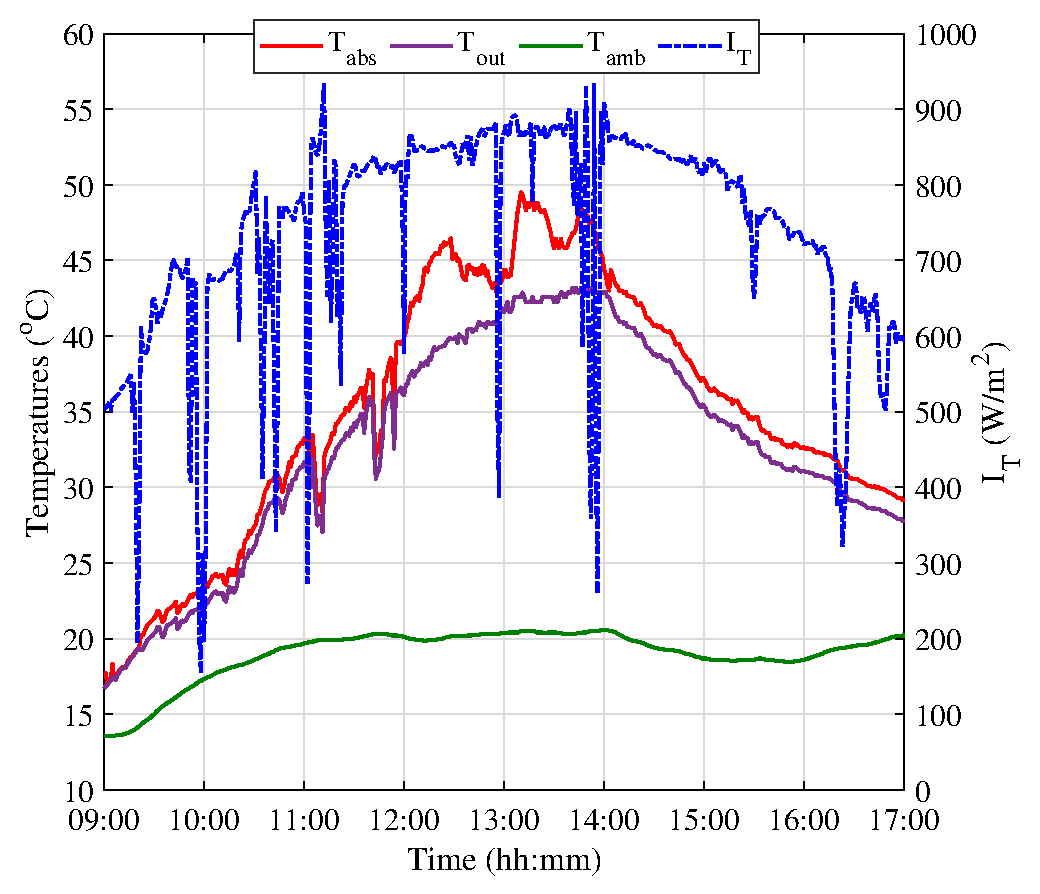
\includegraphics[width=0.98\textwidth]{figs/0055-1.eps} % first figure itself
		\subcaption{Temperature results and solar data.}
	\end{minipage}\hfill
	\begin{minipage}{0.49\textwidth}
		\centering
		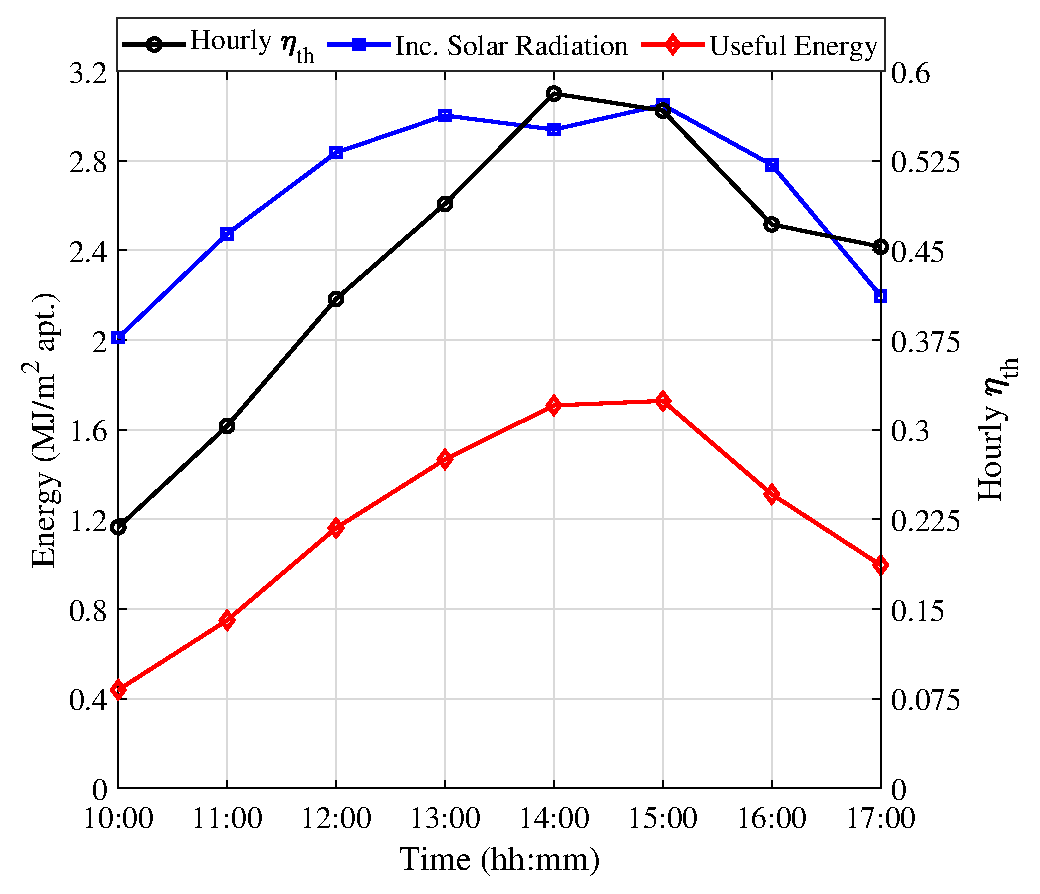
\includegraphics[width=0.98\textwidth]{figs/0055-2.eps} % second figure itself
		\subcaption{Hourly performance and solar data.}
	\end{minipage}
	
	\caption{Experimental results from 22$^{\rm{nd}}$ June at 0.054 kg/(s m$^2$).}
	\label{0055}
\end{figure}

The experimental results of the test operating at medium airflow (0.07 kg/m$^2$.s) are shown in Figure \ref{007} on 29$^{\rm{th}}$ May, in relatively clear sky conditions. The highest $\rm{T_{out}}$ was measured to be 41 $^{\rm{o}}$C  when $\rm{T_{amb}}$ was 21 $^{\rm{o}}$C. The maximum airflow temperature rise was 20 $^{\rm{o}}$C observed between 13:00 and 14:00. The thermal efficiency ($\eta_{\rm{th}}$) in this region was 58\%. The total incident solar energy available on this day was 21.4 MJ/m$^2$; the total useful energy collected was 10.03 MJ/m$^2$, and the average thermal efficiency obtained was 46\%. In the hour of highest solar radiation, the airflow collected 1.7 MJ/m$^2$ of energy at an average $\rm{T_{out}}$ of 40 $^{\rm{o}}$C.


\begin{figure}[!ht]
	\centering
	\begin{minipage}{0.49\textwidth}
		\centering
		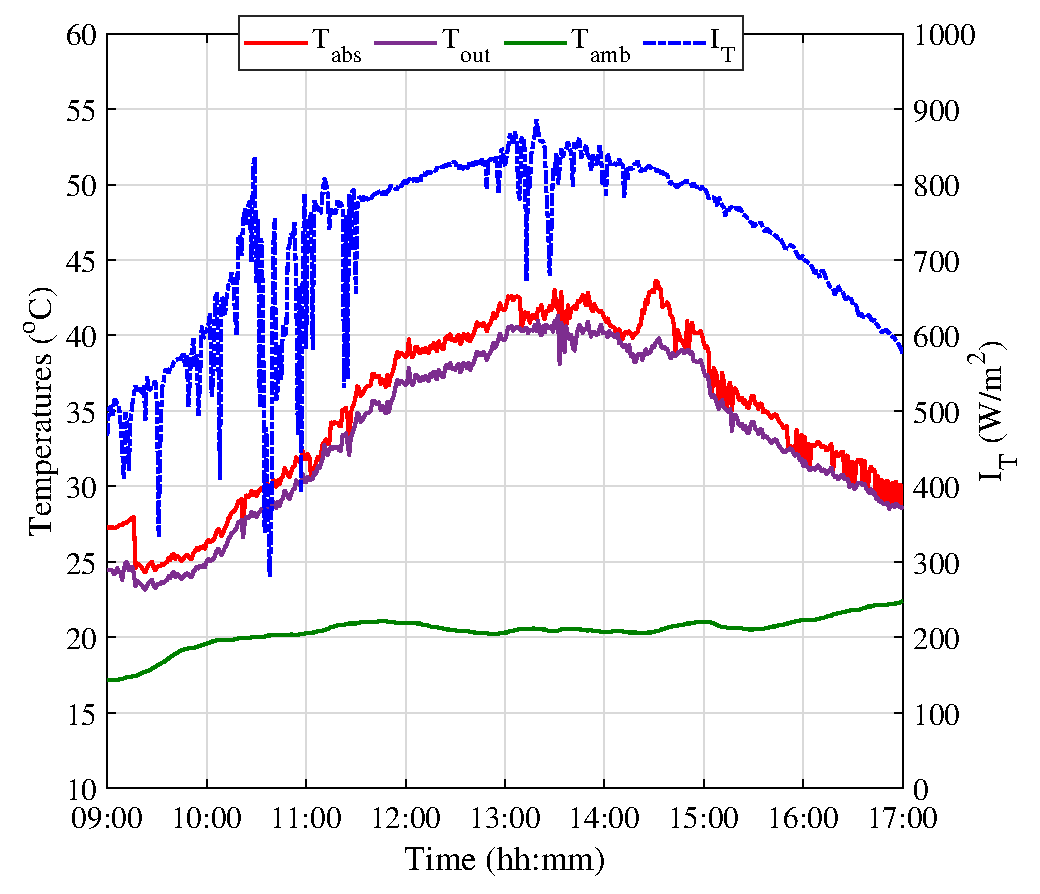
\includegraphics[width=0.98\textwidth]{figs/007-1.eps} % first figure itself
		\subcaption{Temperature results and solar data.}
	\end{minipage}\hfill
	\begin{minipage}{0.49\textwidth}
		\centering
		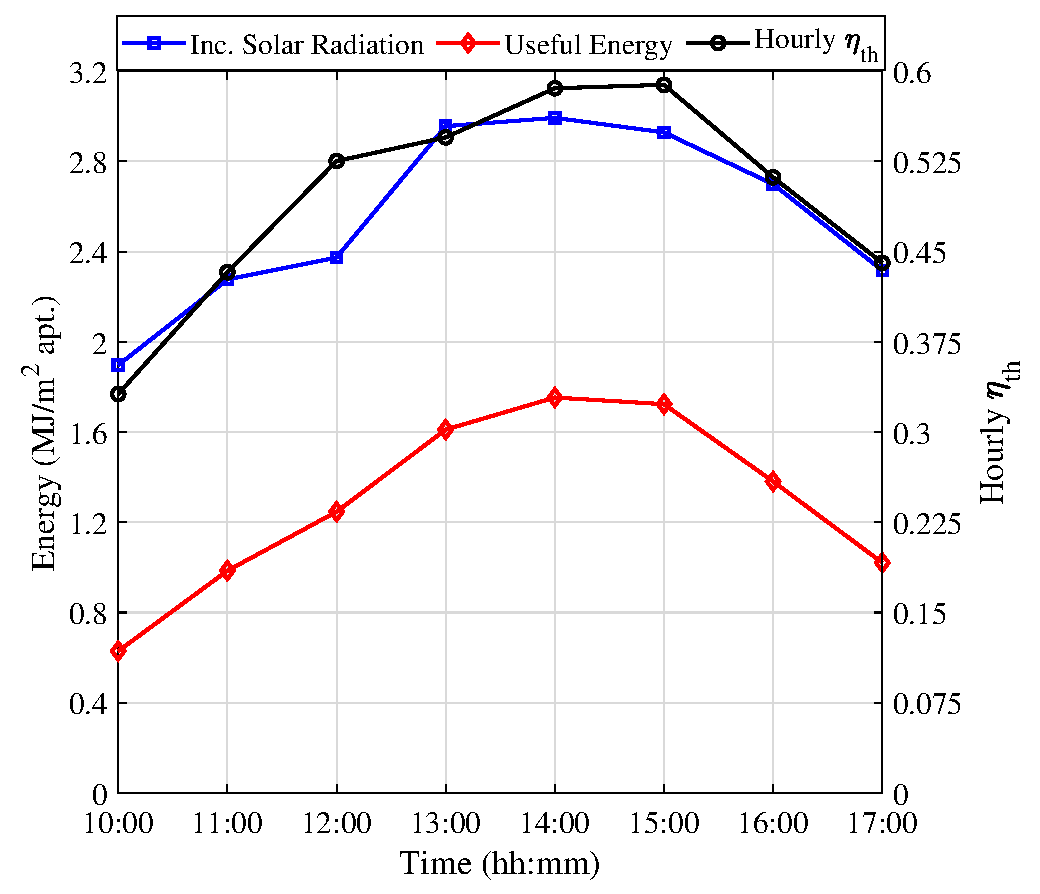
\includegraphics[width=0.98\textwidth]{figs/007-2.eps} % second figure itself
		\subcaption{Hourly performance and solar data.}
	\end{minipage}
	
	\caption{Experimental results from 29$^{\rm{th}}$ May at 0.071 kg/(s m$^2$).}
	\label{007}
\end{figure}

\newpage
The results of the test at med-high airflow (0.089 kg/m$^2$.s) are shown in Figure \ref{009} on 31$^{\rm{st}}$ May. Although the solar data is very transient on this day, $\rm{T_{out}}$ kept constant around 39 $^{\rm{o}}$C  when $\rm{T_{amb}}$ was 23 $^{\rm{o}}$C at solar noon hour. The maximum airflow temperature rise was 16 $^{\rm{o}}$C at the same hour. The thermal efficiency in this region was 59\%. The total solar radiation available was 15.6 MJ/m$^2$, $\rm{Q_{u}}$ was 7.18 MJ/m$^2$, and the average thermal efficiency obtained was 46\%. In the hour with highest solar radiation, the airflow collected 1.6 MJ/m$^2$ of energy at an average $\rm{T_{out}}$ of 39 $^{\rm{o}}$C.


\begin{figure}[!ht]
	\centering
	\begin{minipage}{0.49\textwidth}
		\centering
		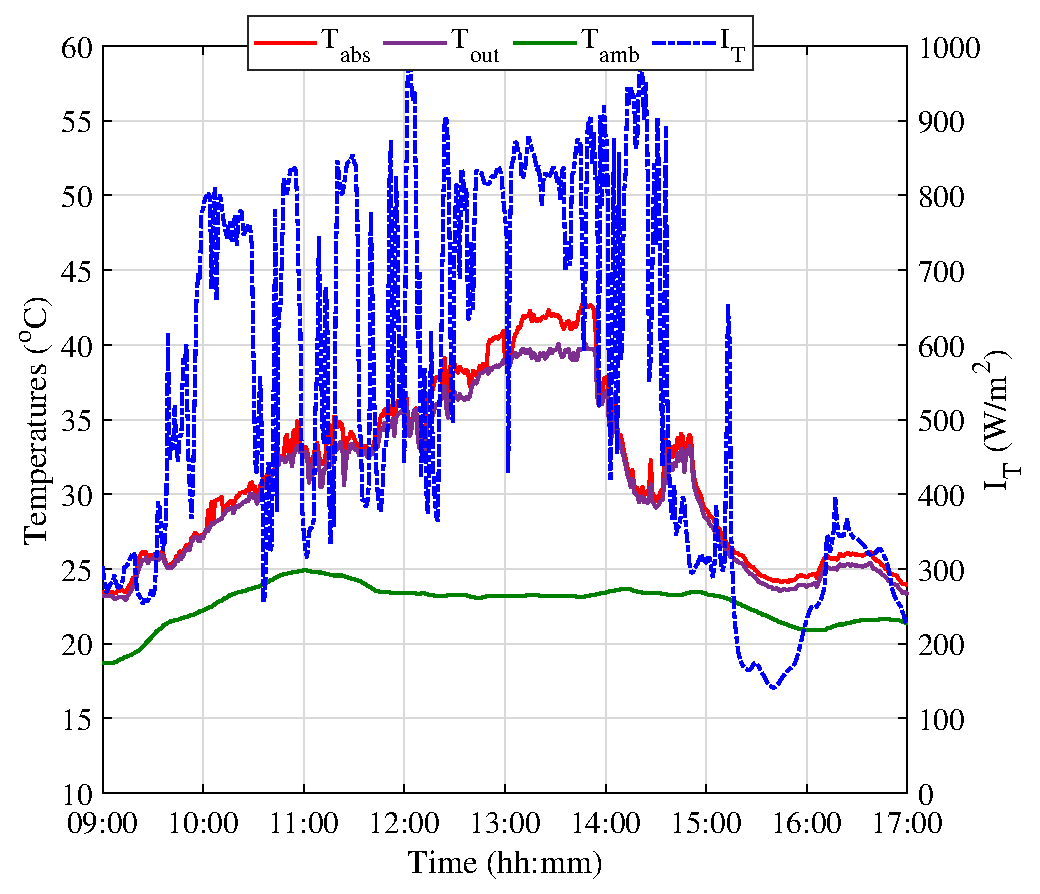
\includegraphics[width=0.98\textwidth]{figs/009-1.eps} % first figure itself
		\subcaption{Temperature results and solar data.}
	\end{minipage}\hfill
	\begin{minipage}{0.49\textwidth}
		\centering
		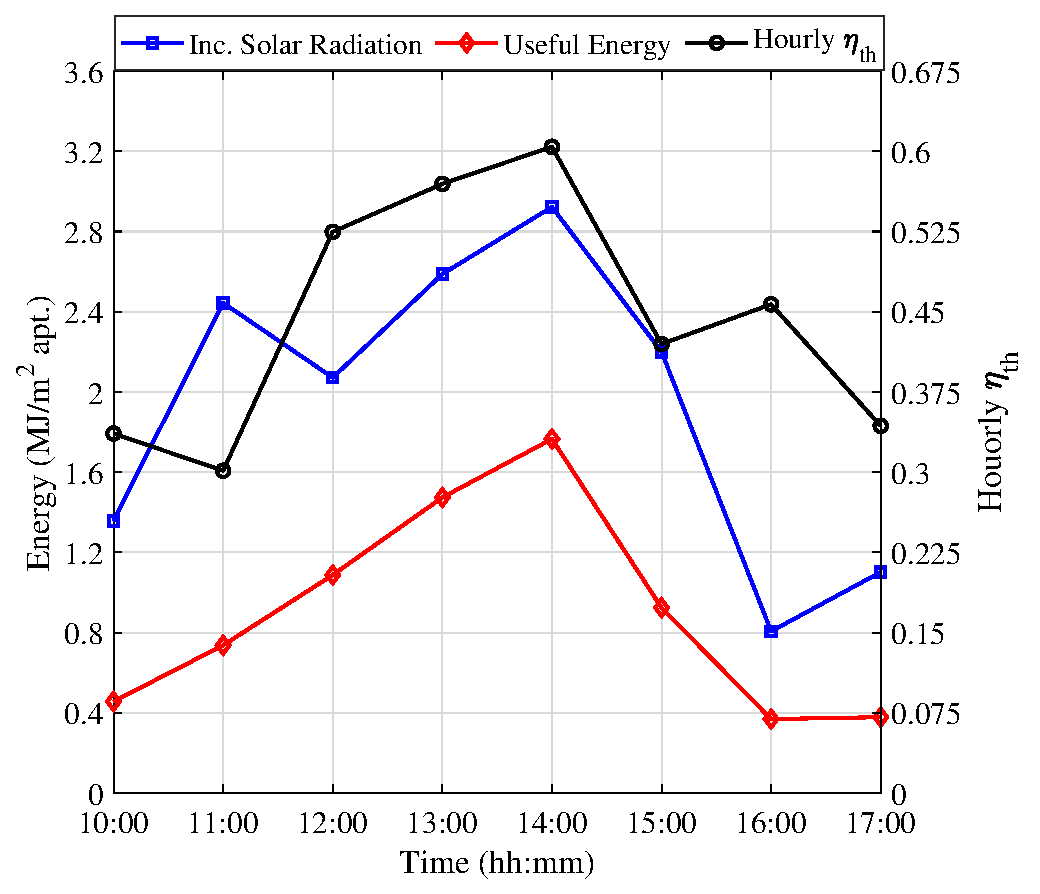
\includegraphics[width=0.98\textwidth]{figs/009-2.eps} % second figure itself
		\subcaption{Hourly performance and solar data.}
	\end{minipage}
	
	\caption{Experimental results from 31$^{\rm{st}}$ May at 0.089 kg/(s m$^2$).}
	\label{009}
\end{figure}

The results of a high airflow rate (0.114 kg/m$^2$.s) experiment are presented in Figure \ref{0115}. It was tested on June 28$^{\rm{th}}$ under clear sky conditions with the highest solar radiation values at the expected solar noon hour, where its peak was 850 W/m$^2$. During this hour, the average values of $\rm{T_{out}}$, $\rm{T_{amb}}$, and $\eta_{\rm{th}}$ were 38 $^{\rm{o}}$C, 27 $^{\rm{o}}$C, and 0.62, respectively. At around the peak of solar radiation, the maximum $\rm{T_{out}}$ was found to be 39 $^{\rm{o}}$C, resulting in the maximum airflow temperature rise of 12 $^{\rm{o}}$C and a corresponding $\eta_{\rm{th}}$ of 0.65. The total incident solar radiation during the test was estimated to be 21.07 MJ/m$^2$, of which the total useful energy collected $\rm{Q_{u}}$ was 9.8 MJ/m$^2$, resulting in a daily thermal efficiency of 0.47.

\begin{figure}[!ht]
	\centering
	\begin{minipage}{0.49\textwidth}
		\centering
		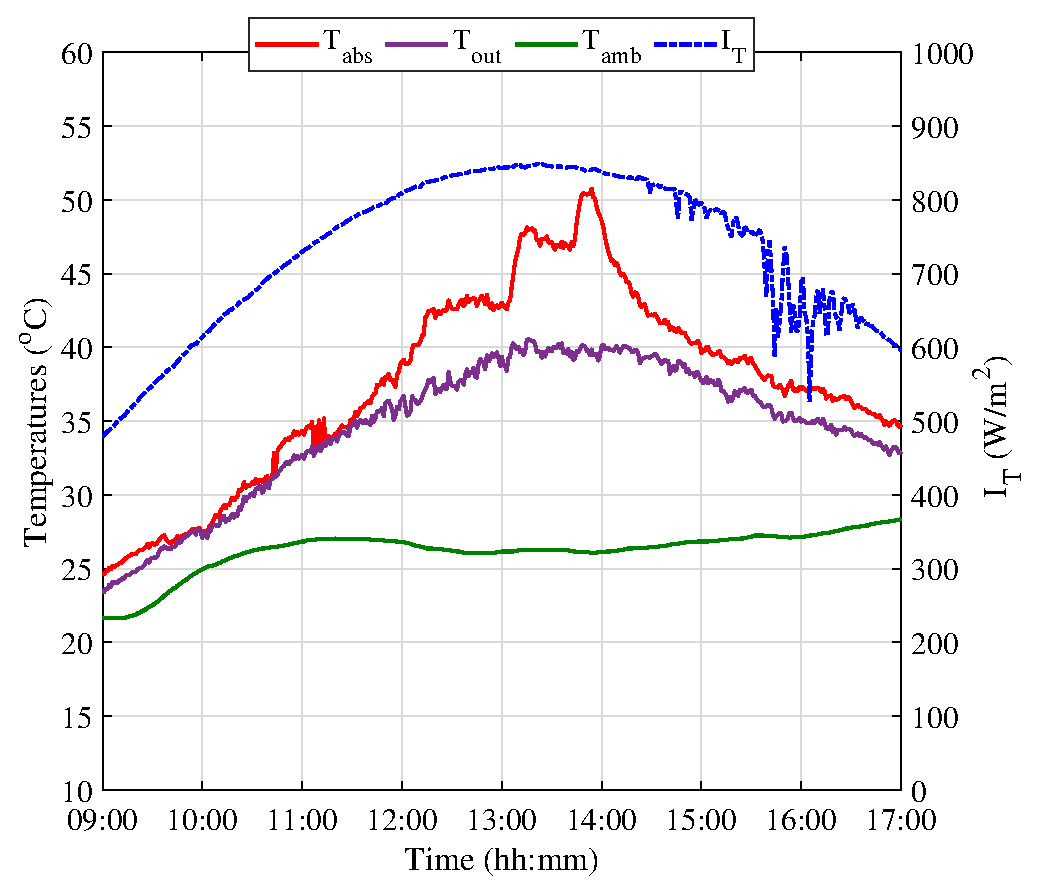
\includegraphics[width=0.98\textwidth]{figs/0115-1.eps} % first figure itself
		\subcaption{Temperature results and solar data.}
	\end{minipage}\hfill
	\begin{minipage}{0.49\textwidth}
		\centering
		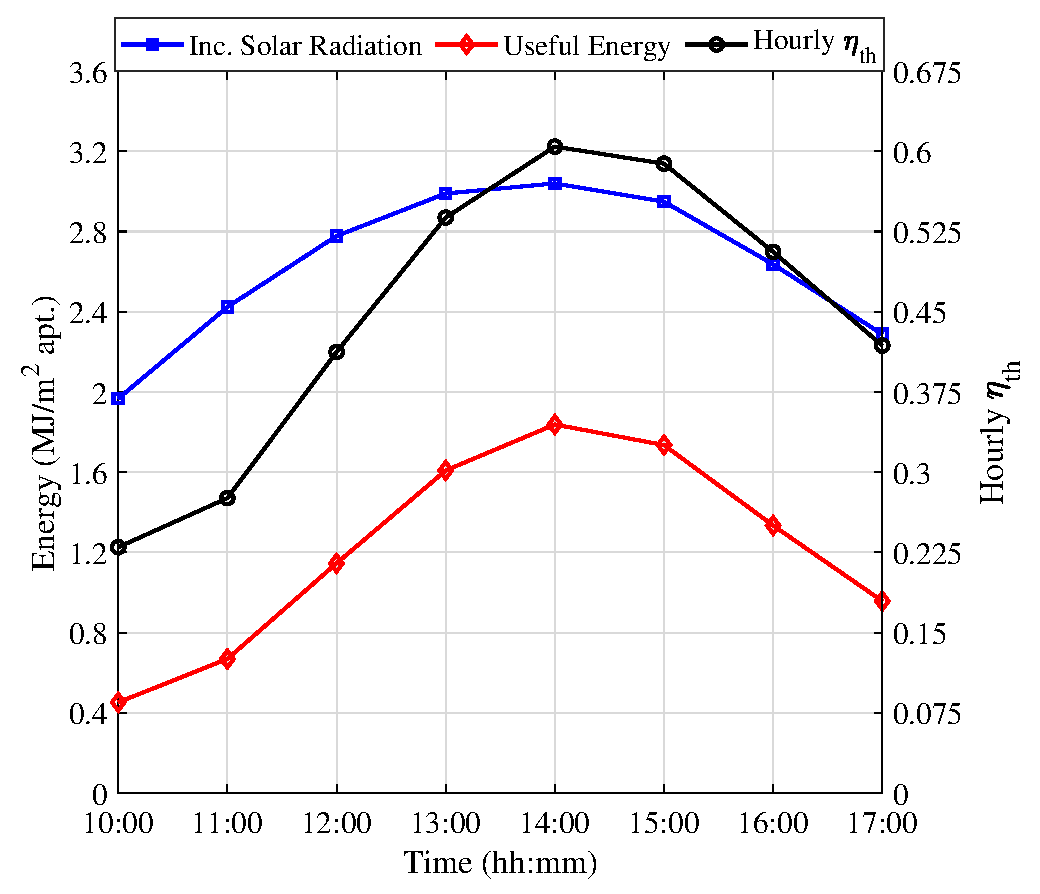
\includegraphics[width=0.98\textwidth]{figs/0115-2.eps} % second figure itself
		\subcaption{Hourly performance and solar data.}
	\end{minipage}
	
	\caption{Experimental results from 28$^{\rm{th}}$ June at 0.114 kg/(s m$^2$).}
	\label{0115}
\end{figure}

\newpage
\subsection{Experimental characterisation at nearly steady state}

The thermal characterisation of solar air heating relates the thermal efficiency under a steady state to each temperature rise normalised by the corresponding solar radiation according to the Hottel-Whillier-Bliss equation, expressed by Eq. (\ref{hottel-whiller-eq2}).

\vspace{-0.75cm}
\begin{equation}
\mathrm{\eta_{\rm{th}} = {F_{\!_R}}\eta_o - {F_{\!_R}}{U_{\!_L}}\frac{(T_{out} - T_{amb})}{I_{\!_T}}}
\label{hottel-whiller-eq2}
\end{equation}

\noindent where $\rm{F_{\!_R}}$ is the heat removal factor. From this equation, $\eta_{\rm{th}}$ can be plotted against $\rm{(T_{out} - T_{amb})/I_{\!_T}}$, resulting in a linear curve, with $\rm{F_{\!_R}}\eta_{\rm{o}}$ and $\rm{- F_{\!_R}{U_{\!_L}}}$ as the linear coefficient and the slope, respectively (\cite{Goswami2015}). 
%From this, the maximum thermal efficiency is $\rm{F_{\!_R}}\eta_{\rm{o}}$ when all the radiation absorbed is transferred to the airflow, but at no temperature change.

The experimental data collected for this analysis were during 10 minutes of tests around the solar noon period of clear days (nearly steady state condition), including all five airflow rates. This is when the direct radiation range is at a maximum of 800 -- 900~W/m$^{\rm{2}}$. To minimise the effects of the system's heat capacity, the data were taken in nearly symmetrical pairs, one before and one after noon, thus resulting in five averaged pairs for each day of experimental tests (\cite{Duffie2013}). Thermal efficiency was calculated by Eq. (\ref{ThermalEf0}). With all the data collected, the thermal efficiency curve was plotted in Figure \ref{ef_curve}. 

\Figure[scale=0.50,placement=!ht,label={ef_curve},caption={Hottel-Whillier-Bliss collector characterisation.}]{figs/exp_curve.eps}

\newpage
From these results, the parameters of Eq. (\ref{hottel-whiller-eq2}) were calculated: $\rm{F_{\!_R}}\eta_{\rm{o}}$ and $\rm{F_{\!_R}{U_{\!_L}}}$ are 0.652 $\pm$ 0.008 and -3.383 $\pm$ 0.328 respectively, and the coefficient of correlation is 0.8. It is important to state that $\rm{U_{\!_L}}$ is assumed to be weakly dependent on the absorber temperature in this operational range, where $\rm{(T_{out} - T_{amb})/I_{\!_T}}$ is between 0.015 and 0.037~m$^{\rm{2}}$.$^{\rm{o}}$C/W, so that the heat loss coefficient is constant (\cite{Rabl1985}). Compared to other work, \citet{Shams2016} characterised experimentally a solar air heating system with a similar geometry. They calculated the instantaneous thermal efficiency when the solar radiation varied between 937.6 and 1,085.4 W/m$^{\rm{2}}$. This resulted in a linear coefficient ($\rm{F_{\!_R}}\eta_{\rm{o}}$) of 0.73 and slope ($\rm{F_{\!_R}{U_{\!_L}}}$) of -3.25 W/m$^{\rm{2}}$.$^{\rm{o}}$C. The experimental results presented were influenced by varying ambient temperatures, as tests were conducted on days with different ambient conditions. The data were not normalized to account for these variations, which may have led to fluctuations in the observed response variables. Future studies could apply normalization techniques to improve comparison of results across different climatic conditions.

Next, Figure \ref{ef-Tout-Gair} shows thermal efficiency and outlet air temperature as functions of the mass airflow rate. From the thermal efficiency graph, it is possible to view a smooth increase in $\eta_{\rm{th}}$ when $\rm{G_{air}}$ becomes higher. The opposite behaviour is observed in the airflow temperature rise $(\rm{T_{out}} - \rm{T_{in}})$, where this variable dramatically drops when $\rm{G_{air}}$ varies from 0.04 to 0.09 kg/m$^2$.s and then falls smoothly by 2 $^{\rm{o}}$C.

\begin{figure}[ht!]
	\begin{minipage}{0.49\columnwidth}
		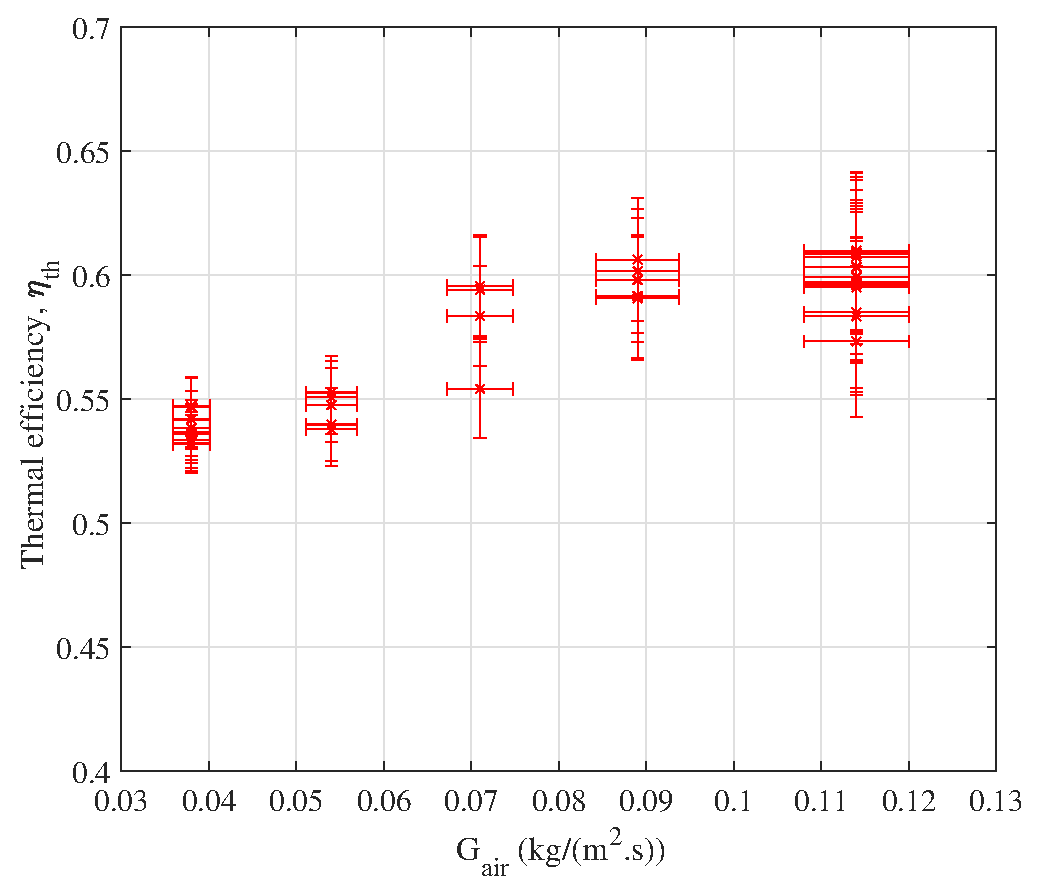
\includegraphics[width=0.98\columnwidth,height=6cm]{figs/ef-Gair2.eps}
		\subcaption{$\eta_{\rm{th}}$ vs. $\rm{G_{air}}$.}
	\end{minipage}
	\begin{minipage}{0.49\columnwidth}
		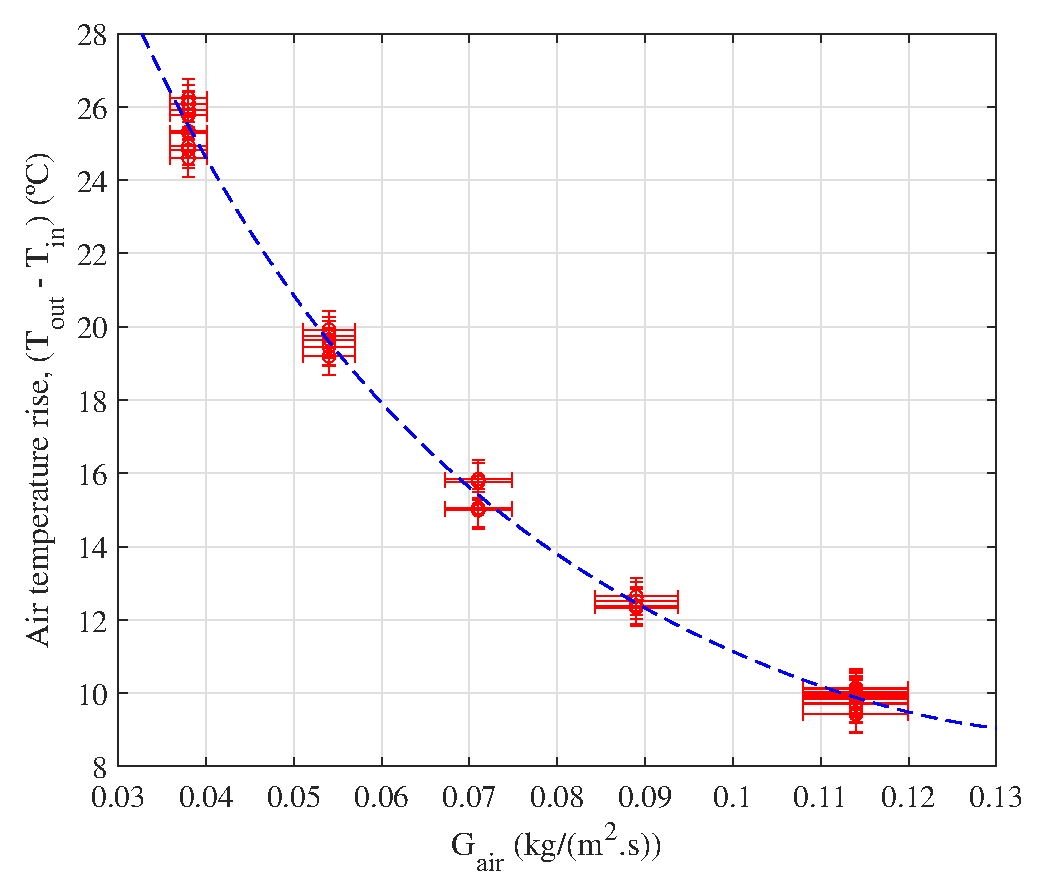
\includegraphics[width=0.98\columnwidth,height=6cm]{figs/dT-Gair2.eps}
		\subcaption{$\rm{(T_{out} - T_{in})}$ vs. $\rm{G_{air}}$.}
	\end{minipage}
    \caption{Graphs of thermal efficiency (a), and airflow temperature rise (b) at different airflow rates at nearly steady state condition.}
	\label{ef-Tout-Gair}
\end{figure}

%\subsection{Comparison of thermal performances}

%\citet{Koyuncu2006} tested 





\section{Chapter summary}

The fabrication of a solar air heating prototype for outdoor experimental tests has been detailed in this chapter. It outlined the selection of materials, the fabrication process and the data collection apparatus. Considering its material properties and the inherent perforation, carbon fibre weave with 85\% absorptivity was selected as the collector's absorber surface. 95\% reflectivity \textit{Mirosun} reflector sheet from the company Alanod was selected as the reflector material. A 4-mm thick tempered clear glass with 90\% transmittance was selected as the glazing cover.

The experiments were conducted in an open-loop configuration, where air was blown by a 12-W fan with a voltage adaptor to vary the airflow rate. Experimental results were obtained for airflow rates ranging from 0.038 to 0.115 kg/(m$^2$.s). Results show that the maximum outlet air temperatures at solar noon (13:00 to 14:00) varied from 40 $^{\rm{o}}$C at the highest airflow to 52 $^{\rm{o}}$C at the lowest and the thermal efficiency varied from 52\% to 62\%. 

Results were also evaluated at nearly steady-state conditions, where the maximum solar radiation range was at solar noon, 800 -- 900 W/m$^{\rm{2}}$. The thermal efficiency curve was plotted to characterise the system. The parameters of the Hottel-Whillier-Bliss equation were calculated: $\rm{F_{\!_R}}\eta_{\rm{o}}$ and $\rm{F_{\!_R}{U_{\!_L}}}$ are 0.65 and -3.39, respectively. The air temperature rise varied from 10~$^{\rm{o}}$C at the highest airflow rate to 26~$^{\rm{o}}$C at the lowest.







	\chapter{Heat Transfer Modelling and Simulation}
\label{Cap:Thermal}
%\vspace{-1.0cm}

%Modelling and simulation are important tools used for predicting a solar heating system's performance.

It is desirable to analyse theoretically a new solar energy, any given system before the prototype fabrication (\cite{Tchinda2008}). A thermal model for simulation of a solar air heater is an important tool to predict its long-term performance under different weather conditions (\cite{Shams2013}). Therefore, this chapter aims to: 

\begin{enumerate}[topsep=5pt,partopsep=0pt] \itemsep0pt
	\item develop a heat transfer model to simulate the thermal performance of the proposed solar air heater, when in operation;
	\item validate the model against experimental data from the tests described in Chapter \ref{Cap:Exp}.
	\item determine how to operate and control the collector based on model.
\end{enumerate}

%1) develop a heat transfer modelling to characterise and simulate the thermal performance of the proposed solar air heater in operation, and; 2) learn how to operate and control base on model. 

Consequently, the specific objectives of this chapter are to:

\begin{itemize}[topsep=5pt,partopsep=0pt] \itemsep0pt
	\item simulate the collector under different solar radiation levels and airflow rates;
	%\item Analyse the effect of the tertiary section on the performance;
	\item estimate outlet airflow temperatures;
	\item evaluate the system's thermal efficiency;
	\item determine useful energy delivered to the airflow;
	%\item Gain understanding of the interaction between system inputs, design parameters and system outputs.
\end{itemize}

%The model was simulated under steady and transient state conditions.

%The model envisages to simulate solar radiation; validate the design prior to fabrication; gain understanding of the interaction between system inputs and outputs, and design parameters; and learn how to operate and control based on the simulation.

The model will be employed to gain an insight and understanding of the interactions between system inputs and outputs shown in Figure \ref{block_diagram}. The model algorithm implemented for simulation was created to predict behaviour under transient state conditions. 

%At a later stage a model validation against experimental data (over the summer period using local weather data) will be undertaken by using statistical tools.

%The validated model will then be used to simulate the system's outlet air temperature and the total useful heat collected with several solar air heater connected altogether. The model was simulated under steady and transient state conditions.

\Figure[scale=0.50,placement=!ht,label={block_diagram},caption={Block diagram of the heat transfer model.},shortcaption={Block diagram of the heat transfer model}]{figs/block_diagram.eps}

\section{Solar air heating collector's heat transfer modelling}

The first step for modelling the solar air heating system is to establish what are the collector's components to be modelled for simulation. In this case there are three: the first one is the absorber surface, the second one is the glazing cover, and the last one is the airflow inside the collector. The next step is to state assumptions in order to simplify the model, which are listed as follows:

\begin{itemize}
	\item Solar radiation is incident uniformly over the components' surfaces;
	\item Absorber and glazing temperatures are uniform;
	\item Thermal and physical properties of the components are independent of temperature;
	\item Heat transfer at the reflectors and wooden cavity, and conduction losses are neglected;
	\item Airflow rate is uniform through all the absorber holes;
	%\item There is no interaction between the airflow and the air below the absorber;
\end{itemize}

The following step of the modelling depicts how the energy balance in the components are evaluated according to the following statements:

\begin{equation*}
\left( \begin{array}{l}
{\rm{\ \ \ \ \ \ Rate \ of}}\\
{\rm{\ internal \ energy }}\\
{\rm{\ in \ the \ absorber}}
\end{array} \right) = \left( \begin{array}{l}
{\rm{Absorbed \ solar}}\\
{\rm{\ \ radiation \ in}}\\
{\rm{\ \ the \ absorber}}
\end{array} \right) - \left( \begin{array}{l}
{\rm{\ \ Heat \ losses}}\\
{\rm{from \ absorber}}
\end{array} \right) - \left( \begin{array}{l}
{\rm{Useful \ heat}}\\
{\rm{ rate \ to \ airflow}}
\end{array} \right)
\label{text_equation_ABS}
\end{equation*}
\vspace*{-0.10cm}
\begin{equation*}
\left( \begin{array}{l}
{\rm{\ \ \ \ \ \ Rate \ of}}\\
{\rm{\ internal \ energy }}\\
{\rm{\ in \ the \ glazing}}
\end{array} \right) = \left( \begin{array}{l}
{\rm{Absorbed \ solar}}\\
{\rm{\ \ radiation \ in}}\\
{\rm{\ \ the \ glazing}}
\end{array} \right) + \left( \begin{array}{l}
{\rm{\ \ Heat \ losses}}\\
{\rm{from \ absorber}}
\end{array} \right) - \left( \begin{array}{l}
{\rm{Heat \ losses}}\\
{\rm{from \ glazing}}
\end{array} \right)
\label{text_equation_GLAZ}
\end{equation*}
\vspace*{-0.10cm}
\begin{equation*}
	\left( \begin{array}{l}
		{\rm{\ \ \ \ \ \ Rate \ of}}\\
		{\rm{\ useful \ energy }}\\
		{\rm{\ in \ the \ airflow}}
	\end{array} \right) = \left( \begin{array}{l}
		{\rm{Convective \ heat}}\\
		{\rm{\ transfer \ from \ the \ }}\\
		{\rm{\ \ absorber \ plate}}
	\end{array} \right) - \left( \begin{array}{l}
		{\rm{\ \ Heat \ losses}}\\
		{\rm{from \ airflow \ }} \\
		{\rm{to \ the \ glazing \ }}
	\end{array} \right) 
	\label{text_equation_air}
\end{equation*}

%\noindent where the heat losses are convective and radiative. %Translating the previous expressions into variables, Eqs. (\ref{EBabsorber1}) and (\ref{EBglazing1}) are obtained:

%\begin{equation}
%\mathrm{\frac{{d{U_{abs}}}}{{dt}} = {S_{abs}} - {Q_{\!_{L,1}}} - {Q_u}}
%\label{EBabsorber1}
%\end{equation}
%\vspace*{-0.5cm}
%\begin{equation}
%\mathrm{\frac{{d{U_{glaz}}}}{{dt}} = {S_{glaz}} + {Q_{\!_{L,1}}} - {Q_{\!_{L,2}}}}
%\label{EBglazing1}
%\end{equation}

\noindent where the heat losses are convective and radiative. In order to visualise how these heat rates are placed, Figure \ref{thermal_network} presents the collector's thermal network as an analogy to an electric circuit, where absorber, glazing and air inside the collector are nodes. The energy input here is the total solar radiation $\rm{I_{\!_{T}}}$, and mathematical expressions above each resistor were used to calculate the thermal resistances.

\Figure[scale=0.75,placement=!ht,label={thermal_network},caption={Thermal network to illustrate heat flows in the air heater, where the subscripts C and R refer to convection and radiation, respectively.}, shortcaption={Thermal network to illustrate heat flows in the air heater.}]{figs/resistances.png}

From the absorber node, the circuit path to the the right is the path of heat transfer to the airflow (upper path) and radiative (lower path) heat losses. At the upper path there is also the convective resistance from the airflow to the glazing indicating that there is convective loss inside the collector. Similarly there are losses from glazing to the ambient indicated by the thermal resistances to the right of its node. These heat transfer types will be addressed later. Applying the concept of heat loss rate as the ratio of temperature difference to the corresponding thermal resistance:

%Alternatively, the solar air heater's cross section with the indexes to represent the thermal energy losses is shown in Figure \ref{scheme_collector}.
%
%\Figure[scale=0.60,placement=!ht,label={scheme_collector},caption={Air heater's cross section with indexes for the heat losses.}]{figs/collector_HT.png}

\vspace{-0.75cm}
\begin{equation}
\mathrm{{M_{abs}}{C_{p,abs}}\frac{{d{T_{abs}}}}{{dt}} = {S_{abs}} - \left( {\frac{{{T_{abs}} - {T_{air}}}}{R_{\!_{HX}}} + \frac{{{T_{abs}} - {T_{glaz}}}}{R_{\!_{R1}}}} \right) }
\label{eqabsorber1}
\end{equation}
\vspace*{-0.25cm}
\begin{equation}
\mathrm{{M_{glaz}}{C_{p,glaz}}\frac{{d{T_{glaz}}}}{{dt}} = {S_{glaz}} + \left( {\frac{{{T_{air}} - {T_{glaz}}}}{R_{\!_{C1}}} + \frac{{{T_{abs}} - {T_{glaz}}}}{R_{\!_{R1}}}} \right) - \frac{{{T_{glaz}} - {T_{amb}}}}{{{\displaystyle{\left( {\frac{1}{{{R_{\!_{C2}}}}} + \frac{1}{{{R_{\!_{R2}}}}}} \right)}^{-1}}}}}
\label{eqglazing1}
\end{equation}
\vspace*{-0.25cm}
\begin{equation}
	\mathrm{G_{air}A_{abs}C_{p,air}\frac{dT_{air}}{dt} = \frac{(T_{abs} - T_{air})}{R_{\!_{HX}}} - \frac{(T_{air} - T_{glaz})}{R_{\!_{C1}}}}
	\label{EBair1}
\end{equation}

Substituting the thermal resistances by the mathematical expressions properly and isolating the derivative terms, Eqs. (\ref{EBabsorber2}), Eq. (\ref{EBglazing2}) and Eq. (\ref{EBair2}) are obtained.

\vspace{-0.75cm}
\begin{equation}
\mathrm{\frac{{d{T_{abs}}}}{{dt}} = \frac{1}{{M _{abs}}{C_{p,abs}}} \left[S_{abs} - {h_{\!_{R1}}}{A_{abs}}({T_{abs} - T_{glaz}}) - {h_{\!_{HX}}A_{abs}(T_{abs} - T_{air})} \right]} 
\label{EBabsorber2}
\end{equation}
\vspace*{-0.25cm}
\begin{equation}
\mathrm{\frac{{d{T_{glaz}}}}{{dt}} = \frac{1}{{{M_{glaz}}{C_{p,glaz}}}}}\left[ \begin{array}{l}
\mathrm{{S_{glaz}} + {h_{\!_{R1}}}{A_{abs}}( {{T_{abs}} - {T_{glaz}}} ) + {h_{\!_{C1}}}{A_{abs}}( {{T_{air}} - {T_{glaz}}} )}\\
\mathrm{- ( {{h_{\!_{R2}}} + {h_{\!_{C2}}}} ){A_{glaz}}( {{T_{glaz}} - {T_{amb}}} )}
\end{array} \right]
\label{EBglazing2}
\end{equation}
\vspace*{-0.25cm}
\begin{equation}
	\mathrm{G_{air}A_{abs}C_{p,air}\frac{dT_{air}}{dt} = h_{\!_{HX}}A_{abs}(T_{abs} - T_{air}) - h_{\!_{C1}}A_{abs}(T_{air} - T_{glaz})       }
	\label{EBair2}
\end{equation}

%Lastly, the thermal efficiency, which is the ratio of useful heat rate to the incoming total solar radiation on the aperture, is calculated by Eq. (\ref{ThermalEf}). Such efficiency can be evaluated either instantaneously or as an average over a certain period of time (\cite{Goswami2015}).
%
%\begin{equation}
%\mathrm{\mathlarger{\eta}_{\mathrm{th}} = \frac{Q_u}{I_{\!_T}A_{apt}}}
%\label{ThermalEf}
%\end{equation}

The next subsections describe how the absorbed solar radiation terms, convective and radiative heat transfer coefficients, useful energy rate and outlet air temperature from the thermal model were determined.

\subsection{Absorbed solar radiation terms}

%However, it is not possible to measure the amount of $\rm{G_{\!_{T}}}$ to be absorbed in the elements. Hence, it is necessary to estimate how much of the total solar radiation is absorbed by each element.

%The incident solar radiation on the solar collector's aperture undergoes optical losses on glazing cover and reflectors before it reaches the absorber surface. The optical loss on the glazing surface depends on the incident angle which varies over time of day and the absorption property of the glazing material. The optical efficiency varies based on the proportion of the beam and diffuse radiation for a particular time of the day.

%The total solar radiation ($\rm{I_{\!_{T}}}$) incident on the concentrator's aperture is the sum of the beam ($\rm{I_{\!_{B}}}$) and diffuse ($\rm{I_{\!_{D}}}$) components. However, since only part of the diffuse radiation is exploitable by concentrators, the factor $\xi$ must be defined, as being the fraction of total solar radiation accepted. Assuming that the diffuse distribution is isotropic, this factor can be estimated as (\cite{Prapas1987}):
%
%\begin{equation}
%\mathrm{\xi  = \frac{\displaystyle {\left( {{I_{\!_B}} + \frac{{{I_{\!_D}}}}{C}} \right)}}{{{I_{\!_T}}}}}
%\label{IC}
%\end{equation} 
%
%\noindent and therefore the incoming solar radiation available to reach the absorber surface is assumed to be $\rm{I_{\!_T}\xi}$. 
The portion of total solar radiation undergoes optical losses before it reaches the absorber -- expressed in terms of ${\eta_{\!_{0}}}$ and previously discussed in Chapters \ref{Cap:Lit} and \ref{Cap:Opt}. Hence, $\rm{S_{abs}}$ is given by Eq. (\ref{Sabs}).
%In order to estimate $\rm{S_{abs}}$, it is necessary to regard that the portion of incoming solar radiation goes through optical losses -- expressed in terms of ${\eta_{\!_{0}}}$ and previously discussed in Chapter \ref{Cap:Opt}. Therefore, $\rm{S_{abs}}$ is given by Eq. (\ref{Sabs}).

\vspace{-0.75cm}
\begin{equation}
\mathrm{{S_{abs}} = I_{\!_{T}}\xi A_{apt}\mathlarger{{\eta_{\!_{0}}}}}
\label{Sabs}
\end{equation}

The absorbed solar radiation by the glazing, which is based on the capacity of this component to retain the incoming radiation incident on the aperture, can be expressed as:

\vspace{-0.75cm}
\begin{equation}
\mathrm{{S_{glaz}} = I_{\!_{T}}A_{apt}{\mathlarger{\alpha}_{\mathrm{glaz}}}}
\label{Sglaz}
\end{equation}

\noindent where the glazing absorptivity $\alpha_{\rm{glaz}}$ was also estimated in Chapter \ref{Cap:Opt}.

\subsection{Radiative heat transfer coefficients}

The radiative heat transfer coefficient from the absorber to the glazing $\rm{h_{\!_{R1}}}$ can be evaluated by Eq. (\ref{hr1}):

\vspace{-0.75cm}
\begin{equation}
\mathrm{{h_{\!_{R1}}} = {\varepsilon _{eff}}\sigma \left( {T_{abs}^2 + T_{glaz}^2} \right)\left( {{T_{abs}} + {T_{glaz}}} \right)}
\label{hr1}
\end{equation}

\noindent where $\rm{\varepsilon_{eff}}$ is the effective emissivity, a radiative property developed by \citet{Rabl1976} for a CPC comprised by specular reflectors. Although the solar air heater to be modelled here is not a simple CPC, such methodology of assessing $\rm{h_{\!_{R1}}}$ was used, given the similarity of both geometries. The calculation of $\rm{\varepsilon_{eff}}$ takes into account: the radiative properties of the absorber, reflector and glazing, such as emissivity and reflectivity, and the concentrator's geometric concentration ratio. 
%Given the assumption os constant properties of the elements defined earlier, this effective emissivity assumes a constant value.

The radiative heat transfer coefficient from the glazing to the ambient $\rm{h_{\!_{R2}}}$ was evaluated by Eq. (\ref{hr2}):

\vspace{-0.75cm}
\begin{equation}
\mathrm{{h_{\!_{R2}}} = {\varepsilon _{glaz}}\sigma \left( {T_{glaz}^2 + T_{amb}^2} \right)\left( {{T_{glaz}} + {T_{amb}}} \right)}
\label{hr2}
\end{equation}

\noindent where the glazing is considered to emit radiation to the ambient only, which absorbs all the emitted energy from that, thus acting as a blackbody (\cite{Duffie2013}).

\subsection{Convective heat transfer coefficients}

%The estimation of $\rm{h_{\!_{C1}}}$ takes two stages of heat transfer: the first is from the absorber to the bottom of the tertiary section and the second is from there to the glazing cover. In the first stage, as the hotter surface is at the top inside the cavity, no convective current will be developed naturally, since the lighter mass of air is always above the heavier. Such type of heat transfer is called pure conduction downwards and then the Nusselt number is a unity (\cite{Cengel2005}). Due to this phenomenon, air layers are formed below the absorber surface inside the cavity (indicated in Figure \ref{figTS}). The convective heat transfer coefficient for this stage is given by:
%
%%it is assumed that the air below the absorber within the tertiary section does not circulate naturally. As there is no heat losses to the reflectors and above the absorber, the heat loss can only "escape" downwards in a conductive manner, thus leading to formation of air layers at that location (indicated in Figure \ref{figTS}). Such type of heat transfer is called pure conduction downwards, where the Nusselt number is unity (\cite{Cengel2005}). The convective heat transfer coefficient for this stage is given by:
%
%\begin{equation}
%\mathrm{h_{\!_{C11}} = \frac{{{k_{air}}}}{{{H_{\!_{TS}}}}}Nu_{\!_{C11}} = \frac{{{k_{air}}}}{{{H_{\!_{TS}}}}}}
%\label{hc11}
%\end{equation}
%
%\noindent where the air thermal conductivity $\rm{k_{air}}$ is calculated as (\cite{Rabl1976}):
%
%\begin{equation}
%\mathrm{{k_{air}} = 4.86 \cdot {10^{-4}}T^{0.7}}
%\label{kair}
%\end{equation}
%
%\noindent with $\rm{k_{air}}$ evaluated at the average temperature between $\rm{T_{abs}}$ and $\rm{T_{\!_{TS}}}$.
%
%\Figure[scale=0.65,placement=!ht,label={figTS},caption={Convective heat transfer taking place within the tertiary section and at the surroundings of the glazing (whose coefficients are $\rm{h_{\!_{C11}}}$ and $\rm{h_{\!_{C12}}}$, respectively).}]{figs/figTS.eps}
%
%The second stage involves the heat transfer from the air at the surroundings of the glazing to this component by natural convection. Hence, the convective heat transfer coefficient $\rm{h_{\!_{C12}}}$ is calculated as:
%
%\begin{equation}
%\mathrm{h_{\!_{C12}} = \frac{{{k_{air}}}}{{{{\overline W}_{glaz}}}}Nu_{\!_{C12}} = a{(Ra)^b}}
%\label{hc12a}
%\end{equation}
%
%\noindent where the parameters a and b depend on the geometry and the flow regime (\cite{Cengel2005}). Assuming laminar flow and an average glazing inclination, a = 0.56 and \mbox{b = 1/4} (\cite{Rabl1976}). The Rayleigh number is defined by Eq.(\ref{hc12b}):
%
%\begin{equation}
%\mathrm{Ra = {\frac{{g{\beta_{th}}}}{{\nu_{air}^2}}{{\overline W}_{glaz}}({T_{c}} - {T_{glaz}})\Pr}}
%\label{hc12b}
%\end{equation}
%
%\noindent where: $\rm{T_{c}}$ is the temperature near the glazing assumed to be the average between $\rm{T_{\!_{TS}}}$ and $\rm{T_{glaz}}$ (shown in Figure \ref{figTS}); the volume expansion coefficient $\beta_{\rm{th}}$ is 1/$\rm{T_{c}}$ as the air is considered an ideal gas; the Prandtl number Pr is assumed to be a constant value; and $\rm{\overline W_{glaz}}$ and $\nu_{\rm{air}}$ are the glazing characteristic length and the air kinematic viscosity, respectively, which are calculated as follows:
%
%\begin{equation}
%\mathrm{{\overline W _{glaz}} = \frac{{{L_{col}}{W_{glaz}}}}{{2({L_{col}} + {W_{glaz}})}}}
%\end{equation}
%\vspace*{-0.5cm}
%\begin{equation}
%\mathrm{{\nu_{air}} = {9.76 \cdot 10^{-10}}{T^{1.7}}}
%\label{nuair}
%\end{equation}
%
%\noindent where, in this stage, $\rm{k_{air}}$ and ${\nu_{\rm{air}}}$ is evaluated at $\rm{T_{c}}$.  Substituting Eqs. (\ref{kair}), (\ref{nuair}) and (\ref{hc12b}) in Eq. (\ref{hc12a}) and thus making arrangements, $\rm{h_{\!_{C12}}}$ can be obtained after the above considerations:
%
%\begin{equation}
%\mathrm{{h_{\!_{C12}}} = 14.2{\left( {\frac{{{T_{c}} - {T_{glaz}}}}{{{{\overline W }_{glaz}}}}} \right)^{0.25}}T_{c}^{ - 0.4}}
%\label{hc12}
%\end{equation}
%
%In order to find $\rm{T_{\!_{TS}}}$ and then calculate $\rm{h_{\!_{C11}}}$ and $\rm{h_{\!_{C12}}}$, an auxiliary equation must be proposed. From the thermal network, it is possible to state that the convective heat loss rate from the absorber to the tertiary section bottom is equivalent to the rate from that position to the glazing, which is presented by Eq. (\ref{Qseries}):
%
%\begin{equation}
%\mathrm{{h_{\!_{C11}}}{A_{abs}}({T_{abs}} - {T_{\!_{TS}}}) = {h_{\!_{C12}}}{A_{glaz}}({T_{\!_{TS}}} - {T_{glaz}})}
%\label{Qseries}
%\end{equation}
%
%This non-linear equation has only $\rm{T_{\!_{TS}}}$ as unknown variable. Newton's Method was applied to solve it iteratively (\cite{Hoffman2001}). After finding $\rm{T_{\!_{TS}}}$, the values of $\rm{h_{\!_{C11}}}$ and $\rm{h_{\!_{C12}}}$ are calculated and, finally, the convective heat transfer coefficient $\rm{h_{\!_{C1}}}$ is obtained:
%
%\begin{equation}
%\mathrm{{h_{\!_{C1}}} = \frac{1}{\displaystyle \frac{1}{h_{\!_{C11}}} + \frac{1}{h_{\!_{C12}}}}}
%\label{hc1}
%\end{equation}
%
%It is important to highlight that when $\rm{H_{\!_{TS}}}$ = 0, it would not be possible to calculate $\rm{h_{\!_{C11}}}$. However, this issue can be overcome by making $\rm{h_{\!_{C11}}}$ = 0, replacing $\rm{T_{\!_{TS}}}$ by $\rm{T_{abs}}$ and proceeding to calculate $\rm{h_{\!_{C12}}}$ with no need to apply any iterative method. In this case, $\rm{h_{\!_{C1}}}$ will be equivalent to $\rm{h_{\!_{C12}}}$. 

%\begin{equation}
%\mathrm{T_{\!_{TS}}^{(j+1)} = T_{\!_{TS}}^{(j)} - %\frac{{{F_1}(T_{\!_{TS}}^{(j)})}}{\displaystyle {{{\left. %{\left( {\frac{{d{F_1}}}{{d{T_{\!_{TS}}}}}} \right)} %\right|}_{T_{\!_{TS}}^{(j)}}}}}}
%\label{NRM}
%\end{equation}

%\noindent where j is the iteration step. The function F$_1$ -- which is Eq. (\ref{Qseries}) with its terms rearranged in only one hand side -- and the derivative of f$_1$ in relation to $\rm{T_{\!_{TS}}}$ are evaluated at $\rm{T_{\!_{TS}}^{(j)}}$. The initial guess is always the average between $\rm{T_{abs}}$ and $\rm{T_{glaz}}$. The absolute difference between $\rm{T_{\!_{TS}}^{(j+1)}}$ and $\rm{T_{\!_{TS}}^{(j)}}$ must be smaller than the tolerance level for convergence. 

In order to calculate the heat transfer coefficient from airflow to glazing $\rm{h_{\!_{C1}}}$, it is assumed that the airflow circulating within the collector loses part of its thermal energy to the glazing by convection. Therefore, the estimation of $\rm{h_{\!_{C1}}}$ is given by Eq. (\ref{hc1}) (\cite{Zheng2016}):

\vspace{-0.75cm}
\begin{equation}
\mathrm{{h_{\!_{C1}}} = \frac{k_{air}}{L_{col}}{Nu_{\!_{C1}}} = \frac{{{k_{air}}}}{{{L_{col}}}}\left( {0.664{\rm{Re}}_{\!_{C1}}^{1/2}{\rm{Pr}}^{1/3}} \right)}
\label{hc1}
\end{equation}

\noindent where it is assumed that the air thermal properties are evaluated at the average between $\rm{T_{abs}}$ and $\rm{T_{in}}$; the Reynolds number based on the air velocity at the inlet ($\rm{v_{in}}$) is:

\vspace{-0.75cm}
\begin{equation}
\mathrm{{{\mathop{\rm Re}\nolimits}_{\!_{C1}}} = \frac{{{v_{in}}{L_{col}}}}{{{\mathlarger{\nu}_{air}}}}}
\label{Rec1}
\end{equation}

In order to calculate the heat transfer coefficient from glazing to ambient $\rm{h_{\!_{C2}}}$, it is assumed that the convection loss is forced by the wind. Therefore, the estimation of it is given by Eq. (\ref{wind}) (\cite{Tchinda2008}):

\vspace{-0.75cm}
\begin{equation}
	\mathrm{h_{\!_{C2}} = 2.8 + 3v_w}
	\label{wind}
\end{equation}

%\subsection{Useful energy rate and outlet air temperature}

%The useful heat rate transferred to the airflow is determined by Eq. (\ref{usefulenergy}):
%
%\begin{equation}
%\mathrm{{Q_u} = {G_{air}}{A_{abs}}{C_{p,air}}({T_{out}} - {T_{in}})}
%\label{usefulenergy}
%\end{equation}

%The useful energy rate was given in Eq. (\ref{usefulenergy}). It should be noted that the outlet air temperature is unknown in the modelling. Therefore, understanding heat transfer from the absorber to the airflow becomes necessary to estimate $\rm{T_{out}}$. To do so, another way of assessing $\rm{Q_u}$ is by using fundamentals of heat exchange (\cite{Incropera2006}), which is proposed by means of Eq. (\ref{heatlog}):
%
%\begin{equation}
%\mathrm{{Q_u} = {h_{\!_{HX}}}A_{abs}^{'}\Delta {T_m}}
%\label{heatlog}
%\end{equation}
%
%\noindent where $\rm{A_{abs}^{'}}$ is the absorber surface area excluding holes:
%
%\begin{equation}
%\mathrm{A_{abs}^{'} = A_{abs}(1 - \varphi_p)}
%\label{areap}
%\end{equation}
%
%\noindent and $\rm{\Delta {T_m}}$ is called logarithmic mean temperature difference, which needs to take into account the absorber, inlet and outlet air temperatures, calculated as:
%
%\begin{equation}
%\mathrm{\Delta {T_m} = \frac{{({T_{abs}} - {T_{out}}) - ({T_{abs}} - {T_{in}})}}{{\displaystyle \ln \left({\frac{{{T_{abs}} - {T_{out}}}}{{{T_{abs}} - {T_{in}}}}} \right)}}}
%\label{Tlog}
%\end{equation}
%
%Combining Eqs. (\ref{usefulenergy}) and (\ref{heatlog}), and then isolating $\rm{T_{out}}$, Eq. (\ref{Tair}) is obtained.
%
%\begin{equation}
%\mathrm{{T_{out}} = {T_{abs}} - ({T_{abs}} - {T_{in}})\left[ {1 - \exp \left( { - \frac{{{h_{\!_{HX}}}(1 - \varphi_{p} )}}{{{G_{air}}{C_{p,air}}}}} \right)} \right]}
%\label{Tair}
%\end{equation}

The convective heat transfer coefficient for the air flowing through a perforated plate ($\rm{h_{\!_{HX}}}$) is calculated by the correlation developed by \citet{Kutscher1994} for a normal flow:

\vspace{-0.75cm}
\begin{equation}
\mathrm{{h_{\!_{HX}}} = \frac{{{k_{air}}}}{{{\varphi_h}}}Nu_{h} = \frac{{{k_{air}}}}{{{\varphi_h}}}\left[ {2.75{{\left( {\frac{\ell }{{{\varphi_h}}}} \right)}^{ - 1.2}}{\rm{Re}}_{h}^{0.43}} \right]}
\label{convectionholes}
\end{equation}

\noindent where the hole pitch and the hole diameter at the absorber are calculated based on the hole area $\rm{A_h}$ in Eqs. (\ref{phole}) and (\ref{dhole}), respectively, whereas Figure \ref{pitch} illustrates a drawing of carbon fibre fabric to indicate the geometry parameters used in the modelling. 

\vspace{-0.75cm}
\begin{equation}
\mathrm{\ell = \sqrt{\frac{{{\mathrm{A_h}}}}{\varphi_{\mathrm{p}}}}}
\label{phole}
\end{equation}
\vspace*{-0.25cm}
\begin{equation}
\mathrm{{\varphi_h} = \sqrt{{\mathrm{A_h}}}}
\label{dhole}
\end{equation}

\Figure[scale=0.50,placement=!ht,label={pitch},caption={Carbon fibre magnified image and drawing for indication of geometric parameters.}]{figs/carbonfiber2.png}

Furthermore, the Reynolds number in the holes is:

\vspace{-0.75cm}
\begin{equation}
\mathrm{{{\mathop{\rm Re}\nolimits} _h} = \frac{{{v_h}{\varphi_h}}}{{{\mathlarger{\nu} _{air}}}}}
\label{reynoldshole}
\end{equation}

\noindent with the average air velocity in the holes as:

\vspace{-0.75cm}
\begin{equation}
\mathrm{{v_h} = \frac{{{G_{air}}}}{{{d_{air}}\varphi_p}}}
\label{vh}
\end{equation}

\noindent where the air physical properties $\rm{d_{air}}$, $\rm{k_{air}}$ and $\rm{\nu_{air}}$ were evaluated at a temperature assumed to be the average between $\rm{T_{in}}$ and $\rm{T_{out}}$ so the value of $\rm{h_{\!_{HX}}}$ could be estimated. 

The useful energy rate $\rm{Q_u}$ was given in Eq. (\ref{usefulenergy}). It should be noted that the outlet air temperature is unknown in the modelling. Therefore, understanding heat transfer from the absorber to the airflow becomes necessary to estimate $\rm{T_{out}}$. One way of assessing this temperature is finding $\rm{T_{air}}$ by solving the energy balance equations and assuming that as the average between inlet and outlet temperatures.

\section{Simulation results and model validation}

\subsection{Simulation settings}

After describing all the variables and parameters, the method for solving the system of two ordinary differential equations (ODEs) must be defined, which is the explicit Euler method for initial condition. It derives from the Taylor series truncated at the second term where the solution of the model is fairly accurate for small values of time step $\Delta \mathrm{t}$ (\cite{Hoffman2001}). The ODEs system is then shown in Eq. (\ref{sysEq}):

\vspace{-0.75cm}
\begin{equation}
\left\{ \begin{array}{l}
\mathrm{{T_{abs}}({t_{m + 1}}) = {T_{abs}}({t_m}) + \Delta t \cdot {f_1}({T_{abs}}({t_m}),{T_{glaz}}({t_m}),{T_{air}}({t_m}))}\\
\mathrm{{T_{glaz}}({t_{m + 1}}) = {T_{glaz}}({t_m}) + \Delta t \cdot {f_2}({T_{abs}}({t_m}),{T_{glaz}}({t_m}),{T_{air}}({t_m}))}\\
\mathrm{{T_{air}}({t_{m + 1}}) = {T_{air}}({t_m}) + \Delta t \cdot {f_3}({T_{abs}}({t_m}),{T_{glaz}}({t_m}),{T_{air}}({t_m}))      }
\end{array} \right.
\label{sysEq}
\end{equation}

\noindent where the functions f$_1$, f$_2$ and f$_3$ are the right hand sides of Eqs. (\ref{EBabsorber2}), (\ref{EBglazing2}) and (\ref{EBair2}), respectively. The initial conditions are the data collected at 9 am of each day of experiment and the time step $\Delta \mathrm{t}$ was set as 1 s. The algorithm used for modelling and simulation was implemented in Matlab$^{\circledR}$ and it followed the steps depicted as follows:

%The time step $\Delta \mathrm{t}$ was set as 0.01 s to reduce truncation error. The initial conditions are:

%%\begin{equation*}
%%\left\{ \begin{array}{l}
%%\mathrm{{T_{abs}}(0) = {T_{amb}}}\\
%%\mathrm{{T_{glaz}}(0) = {T_{amb}}}
%%\end{array} \right.
%%\end{equation*} 

%the initial values of $\rm{T_{abs}}$, $\rm{T_{glaz}}$ and $\rm{T_{in}}$ were at ambient temperature $\rm{T_{amb}}$.

%%\noindent and the inlet air temperature $\rm{T_{in}}$ also considered to be at $\rm{T_{amb}}$. 


\begin{description}[before={\setcounter{descriptcount}{0}},font=\bfseries\stepcounter{descriptcount}\thedescriptcount~]
	\item Input geometric parameters, optical efficiency data ($\eta_{\!_{0}}$) and the components' physical properties;
	\item Input solar radiation ($\rm{I_{\!_T}}$), ambient temperature ($\rm{T_{amb}}$), inlet air temperature ($\rm{T_{in}}$) and wind speed ($\rm{v_w}$) data;
	%, $\rm{I_{\!_B}}$ and $\rm{I_{\!_D}}$
	%\item Input optical efficiency data ($\eta_{\!_{0}}$);
	\item Set time step ($\Delta \rm{t}$), simulation time ($\rm{t_{s}}$ = 8h), initial conditions and initiate time index m = 1;
	\item Run current time ($\rm{t_m}$);
	\item Calculate the terms $\rm{S_{abs}}$, $\rm{S_{glaz}}$, $\rm{h_{\!_{R1}}}$, $\rm{h_{\!_{R2}}}$, $\rm{h_{\!_{C1}}}$, $\rm{h_{\!_{C2}}}$ and $\rm{h_{\!_{HX}}}$;
	%\item Initiate iteration step (j) as zero and assume initial guess as $\rm{T_{\!_{TS}}^{(j)}}$;
	%\item Apply Newton's method to calculate $\rm{T_{\!_{TS}}}$;
	%\item Calculate $\Delta \rm{T_{\!_{TS}}}$ = $\lvert \rm{T_{\!_{TS}}^{(j+1)}}$ -- $\rm{T_{\!_{TS}}^{(j)}} \rvert$;
	%\item Check convergence: if $\Delta \rm{T_{\!_{TS}}}$ is smaller than tolerance level (tol), calculate $\rm{h_{\!_{C1}}}$. If not, do $\rm{j = j + 1}$ and go back to step 8;
    %\item Use $\rm{T_{\!_{TS}}}$ to calculate $\rm{h_{\!_{C1}}}$;
	%\item Check if air is flowing through the air heater. If not, go to step 16;
	%\item Initiate iteration step (j) as zero and assume initial guess as $\rm{T_{out}^{(j)}}$;
	%\item Apply Fixed Point Iteration to calculate $\rm{T_{out}}$;
	%\item Calculate $\Delta \rm{T_{out}}$ = $\lvert \rm{T_{out}^{(j+1)}}$ -- $\rm{T_{out}^{(j)}} \rvert$;
	%\item Check convergence: if $\Delta \rm{T_{out}}$ is smaller than tolerance level, use $\rm{T_{out}}(t_m)$ to calculate $\rm{Q_u}(t_m)$ and $\eta_{\rm{th}}(\rm{t_m})$. If not, do $\rm{j = j + 1}$ and go back to step 13;
    %\item Use $\rm{T_{out}}(t_m)$ to calculate $\rm{Q_u}(t_m)$ and $\eta_{\rm{th}}(\rm{t_m})$;
	\item Calculate $\rm{T_{abs}}(t_{m+1})$, $\rm{T_{glaz}}(t_{m+1})$ and $\rm{T_{air}}(t_{m+1})$;
	\item Calculate $\rm{T_{out}}(t_{m+1})$ and $\rm{Q_u}(t_m)$;
	%\item Go to the next time ($\rm{t_{m+1} = t_m + \Delta t}$);
	\item Check if $\rm{t_{m+1}}$ is the final time. If so, end the simulation. If not, do m = m + 1 and go back to step 4.
\end{description}

%\Figure[scale=0.48,placement=!ht,label={flowchart},caption={Simulation procedure flowchart of the thermal modelling.}]{figs/HT_flowchart.eps}

\begin{table}[!ht]
	\caption{Model parameters values used in the heat transfer modelling.}
	\centering
\begin{tabular}{p{1.75cm}p{5.5cm}p{2.5cm}}
	\hline \\[-10pt]
	Symbol & Model parameter & Value \\ [2pt]
	 \hline \\[-12pt]
	$\rm{C_{p,abs}}$ & Absorber heat capacity & 1000 J/(kg K) \\ [2pt]
	
	$\rm{M_{abs}}$ & Absorber mass & 0.075 kg \\ [2pt]
	
	$\rm{A_{abs}^{'}}$ & Absorber area without holes & 0.17 m$^2$ \\ [2pt]
	
	$\varphi_{\rm{p}}$ & Carbon fibre porosity & 4.19\% \\ [2pt]
	
	$\rm{A_h}$ & Hole area & 0.147 mm$^2$ \\ [2pt]
	
	$\ell$ & Hole pitch & 1.87 mm \\ [2pt]
	
	$\varphi_{\rm{h}}$ & Hole diameter & 0.383 mm \\ [2pt]
 
	$\rm{C_{p,glaz}}$ & Glazing heat capacity & 880 J/(kg K) \\ [2pt]
 
	$\rm{M_{glaz}}$ & Glazing mass & 3.7 kg \\ [2pt]
	
    $\rm{n_{glaz}}$ & Glazing refraction index & 1.526 \\ [2pt]
 
	$\rm{K_{ext}}$ & Glaz. extinction coefficient & 4 m$^{-1}$ \\ [2pt]
	
	$\rm{{\overline W}_{glaz}}$ & Glaz. characteristic length & 0.11 m \\ [2pt]
	
	%$\rho_{\rm{ref}}$ & Reflector reflectivity & 0.95 \\ [2pt]

	$\varepsilon_{\rm{eff}}$ & Effective emissivity & 0.68 \\ [2pt]

	$\rm{C_{p,air}}$ & Air heat capacity & 1000 J/(kg K) \\ [2pt]
 
	$\rm{Pr}$ & Prandtl number & 0.72 \\ [2pt]

	$\xi$ & Intercept factor & 0.93 \\ [2pt]
 
	$\Delta {\rm{t}}$ & Time step & 1 s \\ 
	\hline 
\end{tabular}
	\label{model_parameters}
\end{table}

The experimental data were used to validate the heat transfer model. The purpose of validation is to determine if the model is an accurate representation of this air heating system (\cite{Banks1987}). In order to measure the model accuracy in predicting experimental data, an error estimator was used: the mean absolute error (MAE), defined as the percentage mean of absolute errors relative to individual observations. Such estimator is calculated by Eq. (\ref{MAE})(\cite{Pujol-Nadal2015}):

\vspace{-0.75cm}
\begin{equation}
\mathrm{MAE(\% ) = \frac{{100}}{{{N_{obs}}}}\sum\limits_{i = 1}^{{N_{obs}}} {\left| {\frac{{{X_{exp,i}} - {X_{sim,i}}}}{{{X_{exp,i}}}}} \right|} }
\label{MAE}
\end{equation}

\noindent where $\rm{X_{exp,i}}$ is the experimental (observed) value and $\rm{X_{sim,i}}$ is the simulated (estimated) value of the same variable. Another way to measure accuracy is to assess the frequency and magnitude of residues (difference between experimental and simulated values) generated by the mathematical model. A positive residue indicates model underestimation while a negative one indicates overestimation.

\subsection{Model validation}

The model validation consisted of comparing the simulated variables $\rm{T_{out}}$ and $\rm{Q_{u}}$ to the experimental ones under the same conditions of the experimental results presented in Chapter \ref{Cap:Exp}.

\subsubsection{Validation of results at low airflow rate}

Figure \ref{004-3}(a) shows the graphs of solar radiation data, experimental and simulated results of the test on 9$^{\rm{th}}$ June ($\rm{G_{air}}$ = 0.04 kg/m$^2$.s), whereas Figures \ref{004-3}(b) and \ref{004-3}(c) present the residue plot in relation to the simulated values. On this clear sky day the calculated MAE for $\rm{T_{out}}$ and $\rm{Q_{u}}$ are 1.9\% and 5.3\%, respectively. During the hour of highest solar radiation (13:00 -- 14:00) the residues are mostly between $\pm$1 $^{\rm{o}}$C and $\pm$20 W/m$^2$. It was found that 70\% of the residues have magnitude of $\pm$1 $^{\rm{o}}$C;  80\% are between $\pm$20 W/m$^2$ and 60\% of the predictions are underestimated (positive residues).

%From Figure \ref{004-3}(b), the maximum relative error is close to 4\% observed in the beginning and end of the day; such error corresponds to 1 $^{\rm{o}}$C of residue. From 11:00 to 13:00 and 14:00 to 15:30 the model prediction underestimates the performance by 2 $^{\rm{o}}$C at most. From Figure \ref{004-3}(c), the maximum relative error is 20\% observed between 09:00 to 10:00; however, this error corresponds only to 20 W/m$^2$ in residue. From 10:00 the model predicts the performance by less than 10\% of relative error, corresponding to 40 W/m$^2$ of underestimation.


\begin{figure}[ht!]
\begin{minipage}{0.60\columnwidth}
		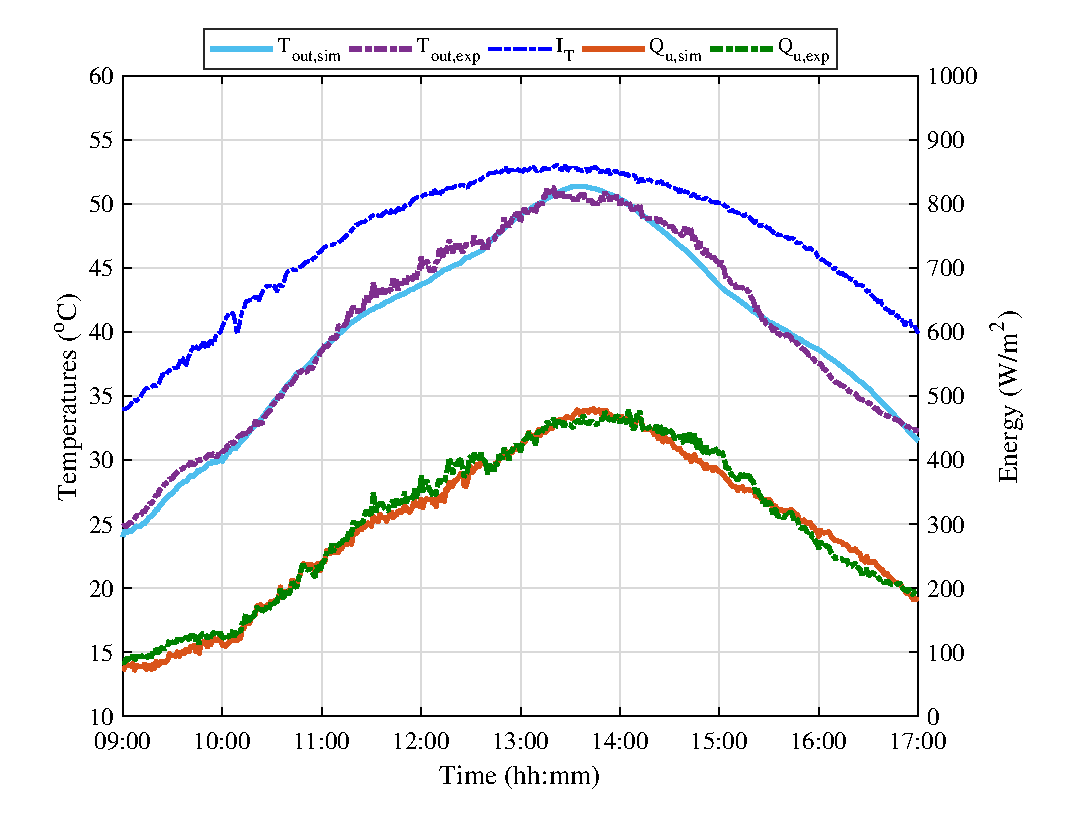
\includegraphics[width=0.99\columnwidth,height=65mm]{figs/004-3.eps}
		%\\[-9mm]
		\subcaption{Experimental and simulated results over time.}
	\end{minipage}
	\begin{minipage}{0.39\columnwidth}
		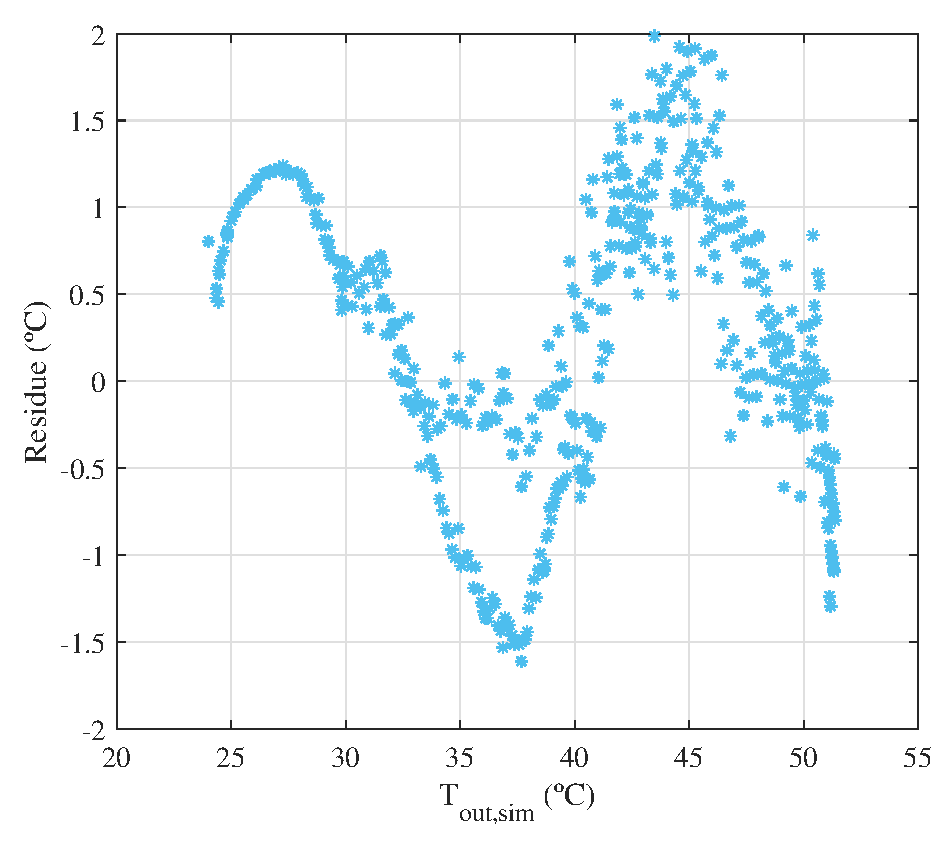
\includegraphics[scale=0.5,width=1.0\columnwidth]{figs/004-residue-5.eps}
		\subcaption{Residue vs. simulated $\rm{T_{out}}$.}
		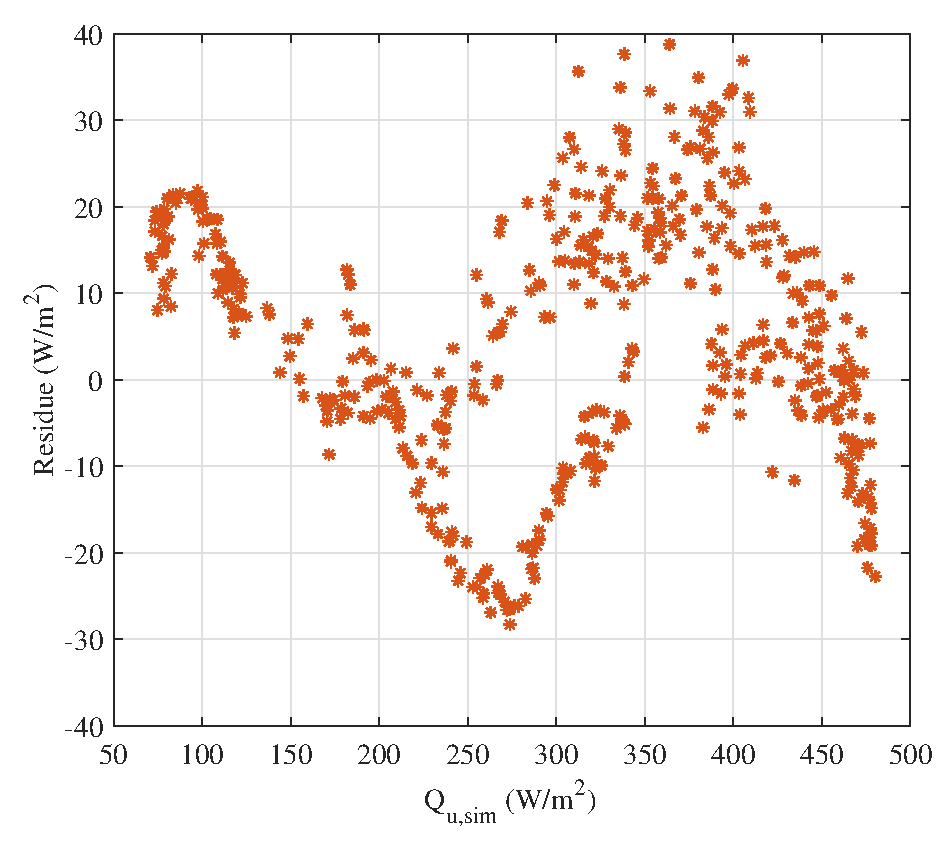
\includegraphics[scale=0.5,width=1.0\columnwidth]{figs/004-residue-6.eps}
		\subcaption{Residue vs. simulated $\rm{Q_{u}}$.}
	\end{minipage}
	
	\caption{(a) Experimental and simulated results, (b) residues of $\rm{T_{out}}$, and (c) residues of $\rm{Q_{u}}$ from 09$^{\rm{th}}$ June at 0.04 kg/(s m$^2$).}
	\label{004-3}
\end{figure}

%\Figure[scale=0.63,placement=!ht,label={004-3},caption={Experimental and simulated results from 09$^{\rm{th}}$ June at 0.04 kg/m$^2$.s. MAE is 2.3\% in terms of $\rm{T_{out}}$ and 7.1\% in terms of $\rm{Q_u}$.}]{figs/004-3.eps}

\subsubsection{Validation of results at low-med airflow rate}

Figure \ref{0055-3}(a) shows solar radiation, experimental and simulated data of the test on 22$^{\rm{nd}}$ June ($\rm{G_{air}}$ = 0.055 kg/(s m$^2$)). On this clear sky day with intermittent clouds, the calculated MAE regarding $\rm{T_{out}}$ and $\rm{Q_{u}}$ are 2.2\% and 6.0\%, respectively. Although it was a day with sudden variation in solar radiation at different moments, the model predicted the outputs which most of the residues are between -0.5 and 1 $^{\rm{o}}$C, and -10 and 30 W/m$^2$, except in two periods: after 16:00, when the decay of $\rm{I_{\!_T}}$ lasted 10 minutes before rising to the natural trend; and shortly before 14:00, when $\rm{I_{\!_T}}$ became highly unstable. These events might explain why the model underestimated the outputs by more than 1.5 $^{\rm{o}}$C and 30 W/m$^2$. From Figures \ref{0055-3}(b) and \ref{0055-3}(c), 85\% of the residues have magnitude of $\pm$1 $^{\rm{o}}$C;  90\% of the residues are between $\pm$30 W/m$^2$ and 88\% of the predictions are underestimated.

%The regions of maximum error is observed in the beginning and in the end of the operation (6\% in $\rm{T_{out}}$ and 20\% in $\rm{Q_u}$). 

\begin{figure}[ht!]
\begin{minipage}{0.60\columnwidth}
		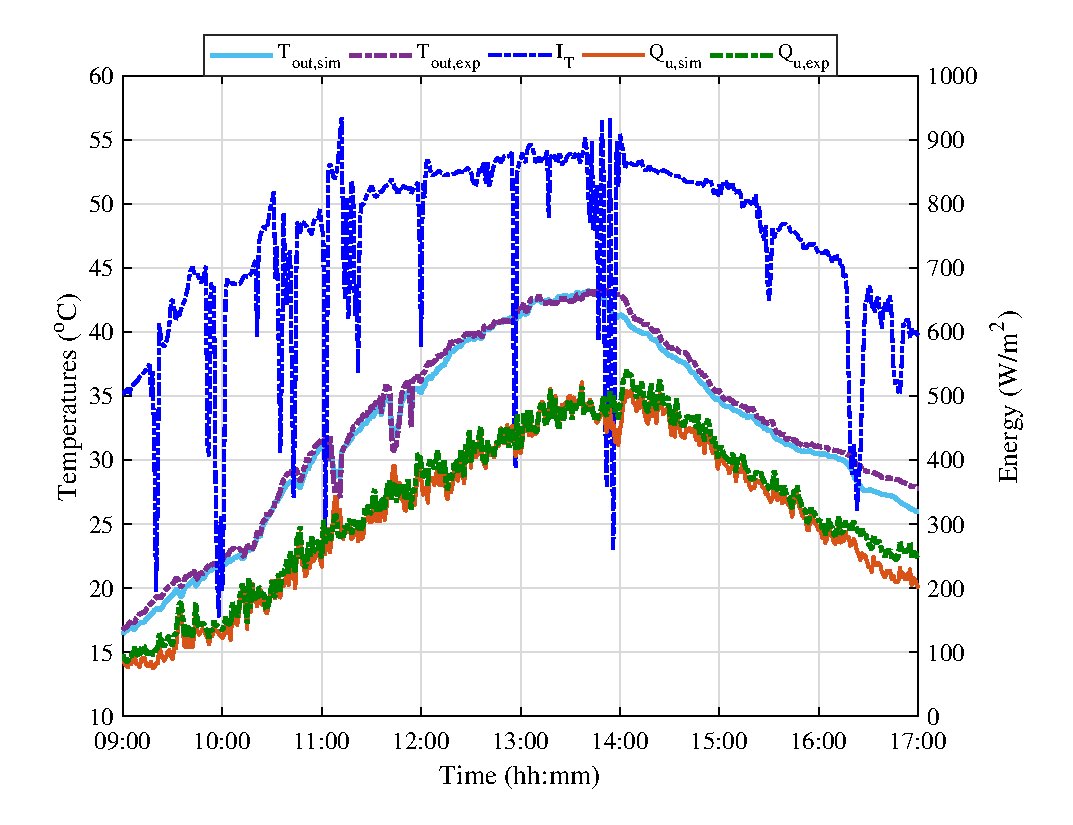
\includegraphics[width=0.99\columnwidth,height=65mm]{figs/0055-3.eps}
		%\\[-9mm]
		\subcaption{Experimental and simulated results over time.}
	\end{minipage}
	\begin{minipage}{0.39\columnwidth}
		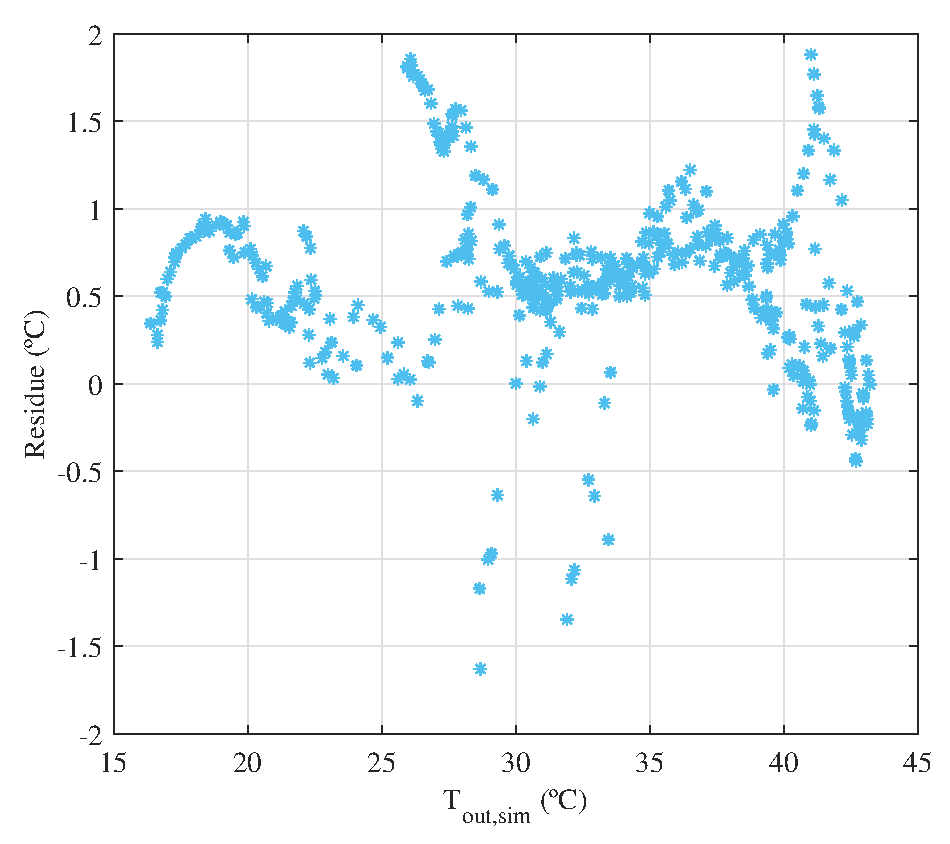
\includegraphics[scale=0.5,width=1.0\columnwidth]{figs/0055-residue-5.eps}
		\subcaption{Residue vs. simulated $\rm{T_{out}}$.}
		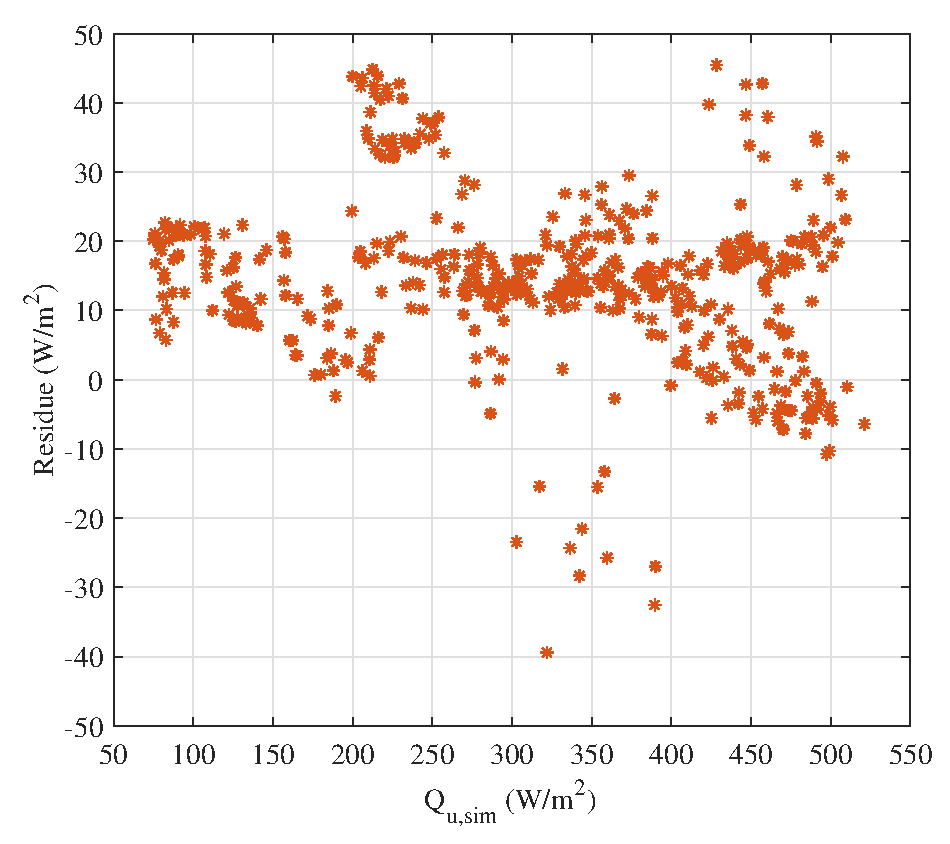
\includegraphics[scale=0.5,width=1.0\columnwidth]{figs/0055-residue-6.eps}
		\subcaption{Residue vs. simulated $\rm{Q_{u}}$.}
	\end{minipage}
	
	\caption{(a) Experimental and simulated results, (b) residues of $\rm{T_{out}}$, and (c) residues of $\rm{Q_{u}}$ from 22$^{\rm{nd}}$ June at 0.055 kg/(s m$^2$).}
	\label{0055-3}
\end{figure}

%\Figure[scale=0.60,placement=!ht,label={0055-3},caption={Experimental and simulated results from 22$^{\rm{nd}}$ June at 0.055 kg/m$^2$.s. MAE is 4.3\% in terms of $\rm{T_{out}}$ and 11.8\% in terms of $\rm{Q_u}$.}]{figs/0055-3.eps}

\subsubsection{Validation of results at medium airflow rate}

Figure \ref{007-3}(a) shows the graphs of solar radiation data, experimental and simulated results of the test on 29$^{\rm{th}}$ May ($\rm{G_{air}}$ = 0.07 kg/m$^2$.s), whereas Figures \ref{007-3}(b) and \ref{007-3}(c) present the residue plot in relation to the simulated values. On this clear sky day with intermittent clouds mainly before 12:00, the calculated MAE for $\rm{T_{out}}$ and $\rm{Q_{u}}$ are 1.6\% and 4.9\%, respectively. The outputs also did not fall substantially due to the solar radiation's sudden variation. In this case, the model underestimated 88\% of the predictions, where 95\% of the residues are between $\pm$1 $^{\rm{o}}$C and 93\% are between $\pm$30 W/m$^2$. It is also noted that the maximum residue is less than 1.2 $^{\rm{o}}$C and less than 40 W/m$^2$. 

\begin{figure}[ht!]
\begin{minipage}{0.60\columnwidth}
		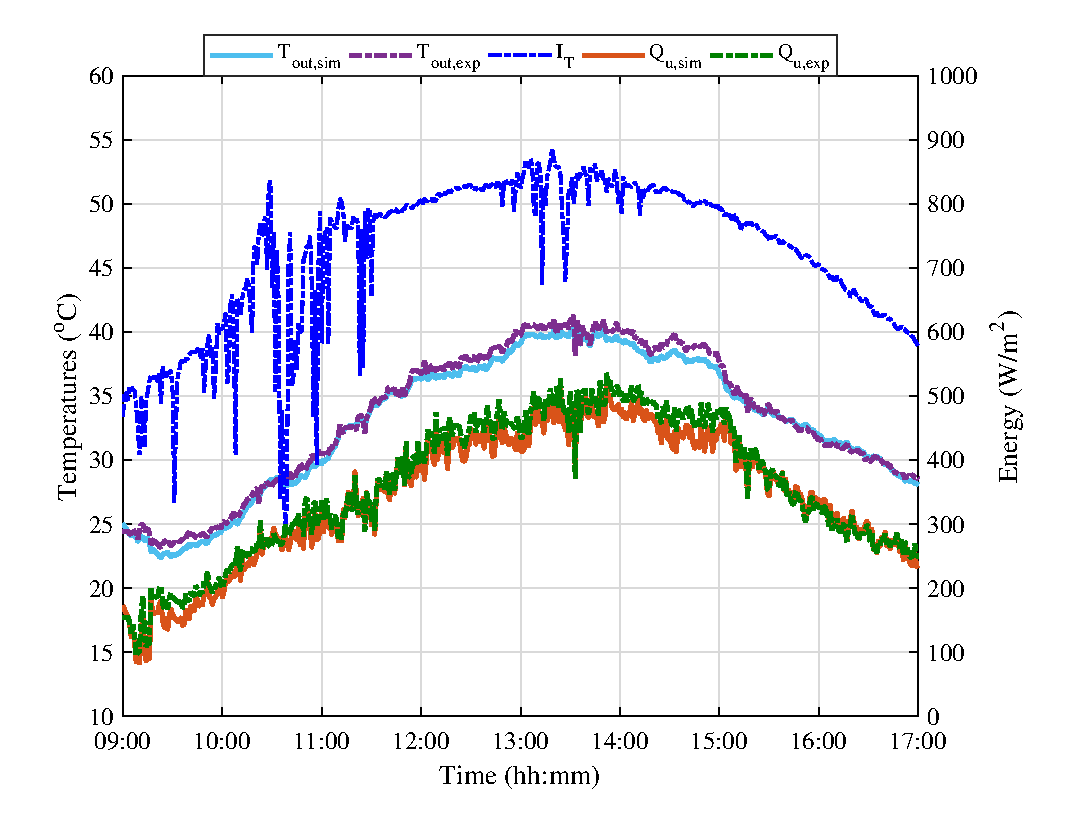
\includegraphics[width=0.99\columnwidth,height=65mm]{figs/007-3.eps}
		%\\[-9mm]
		\subcaption{Experimental and simulated results over time.}
	\end{minipage}
	\begin{minipage}{0.39\columnwidth}
		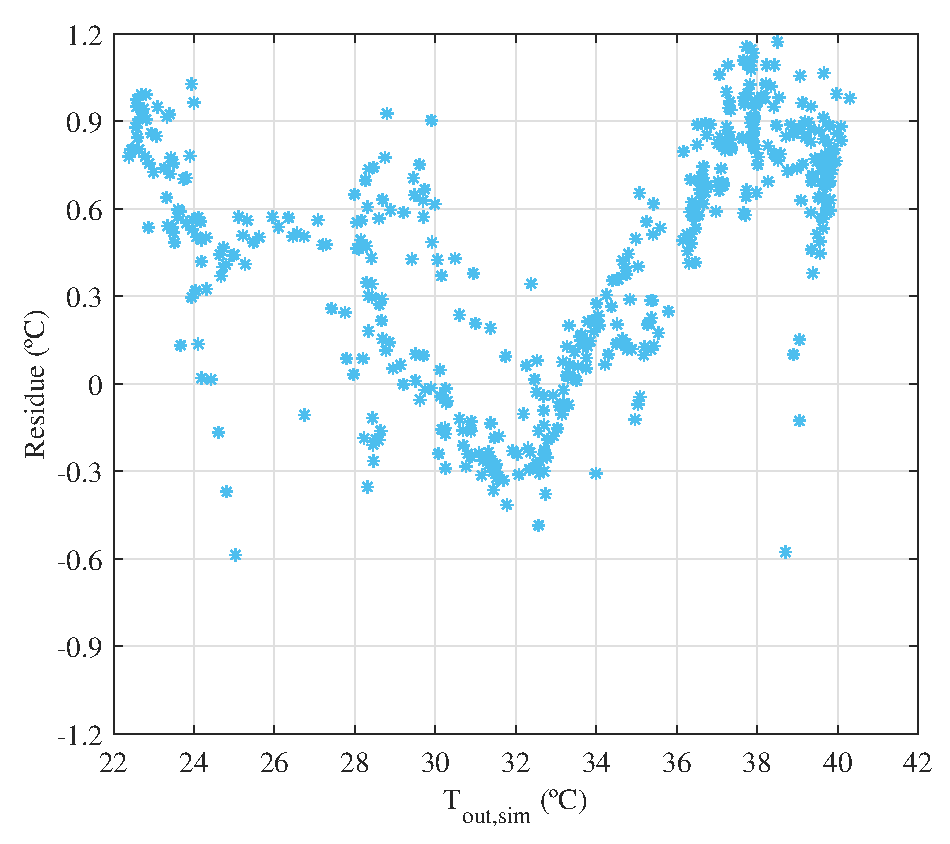
\includegraphics[scale=0.5,width=1.0\columnwidth]{figs/007-residue-5.eps}
		\subcaption{Residue vs. simulated $\rm{T_{out}}$.}
		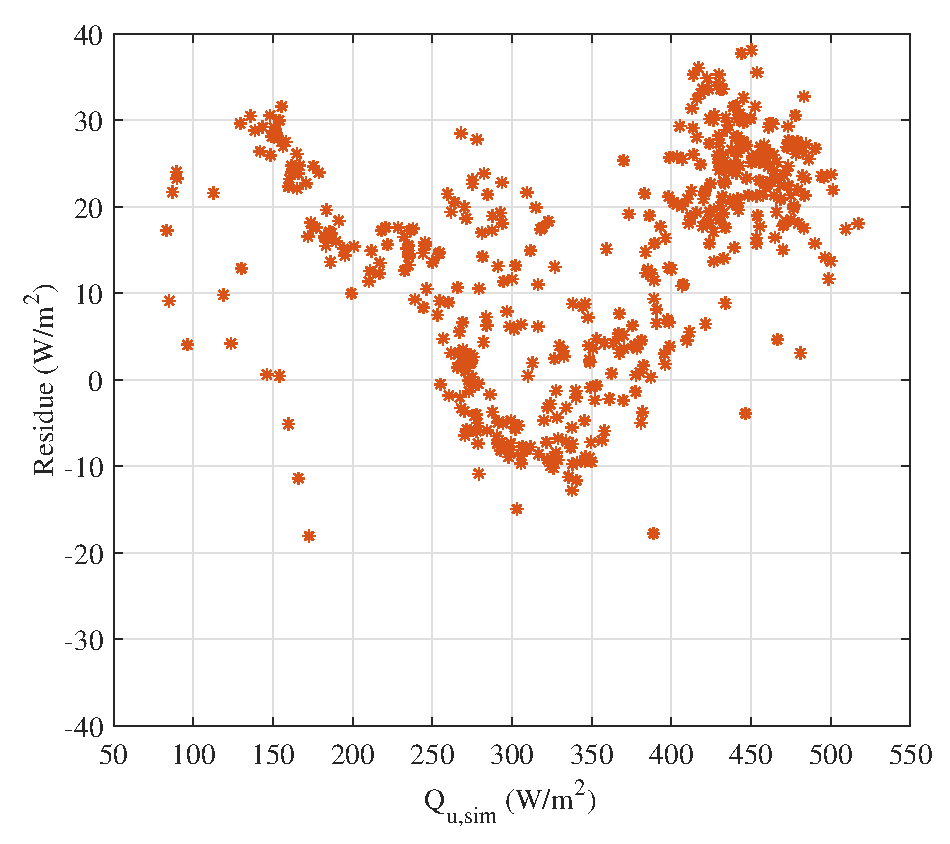
\includegraphics[scale=0.5,width=1.0\columnwidth]{figs/007-residue-6.eps}
		\subcaption{Residue vs. simulated $\rm{Q_{u}}$.}
	\end{minipage}
	
	\caption{(a) Experimental and simulated results, (b) residues of $\rm{T_{out}}$, and (c) residues of $\rm{Q_{u}}$ from 29$^{\rm{th}}$ May at 0.07 kg/(s m$^2$).}
	\label{007-3}
\end{figure}

%\Figure[scale=0.63,placement=!ht,label={007-3},caption={Experimental and simulated results from 29$^{\rm{th}}$ May at 0.07 kg/m$^2$.s. MAE is 6.3\% in terms of $\rm{T_{out}}$ and 19\% in terms of $\rm{Q_u}$.}]{figs/007-3.eps}

\subsubsection{Validation of results at medium-high airflow rate}

Figure \ref{009-3}(a) shows solar radiation, experimental and simulated data of the test on 29$^{\rm{th}}$ May ($\rm{G_{air}}$ = 0.09 kg/m$^2$.s). The calculated MAE for $\rm{T_{out}}$ and $\rm{Q_{u}}$ are 2.5\% and 13.7\%, respectively. The model prediction is the least accurate in this case due to high variations in $\rm{I_{\!_T}}$ throughout the day. From 14:00 to 15:00 the model overestimated the experimental data by more than 2 $^{\rm{o}}$C and more than 56 W/m$^2$ and up to 130 W/m$^2$. This large difference can be due to any unknown experimental fluctuation during the test. From Figures \ref{009-3}(b) and \ref{009-3}(c), the simulated outputs were also underestimated compared to the experimental results in 79\% of the cases. It was found that 70\% of the residues have magnitude of \mbox{$\pm$1 $^{\rm{o}}$C} and 75\% are between $\pm$40 W/m$^2$.

\begin{figure}[ht!]
\begin{minipage}{0.60\columnwidth}
		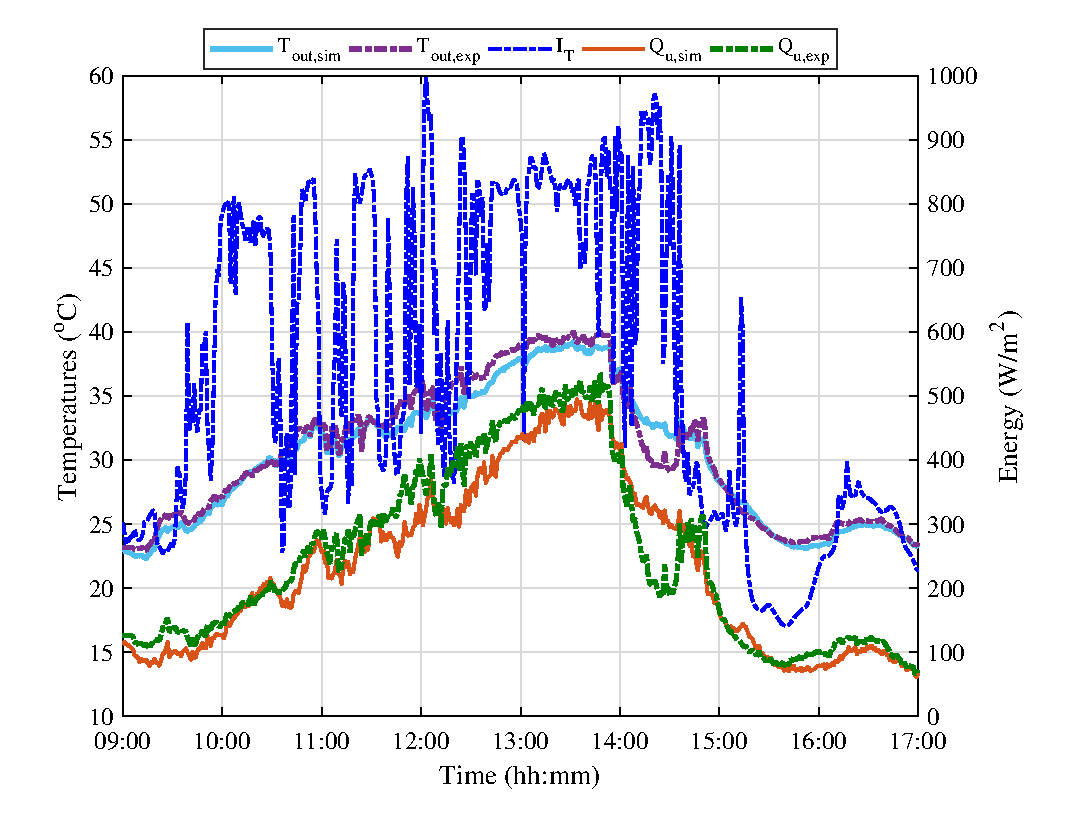
\includegraphics[width=0.99\columnwidth,height=65mm]{figs/009-3.eps}
		%\\[-9mm]
		\subcaption{Experimental and simulated results over time.}
	\end{minipage}
	\begin{minipage}{0.39\columnwidth}
		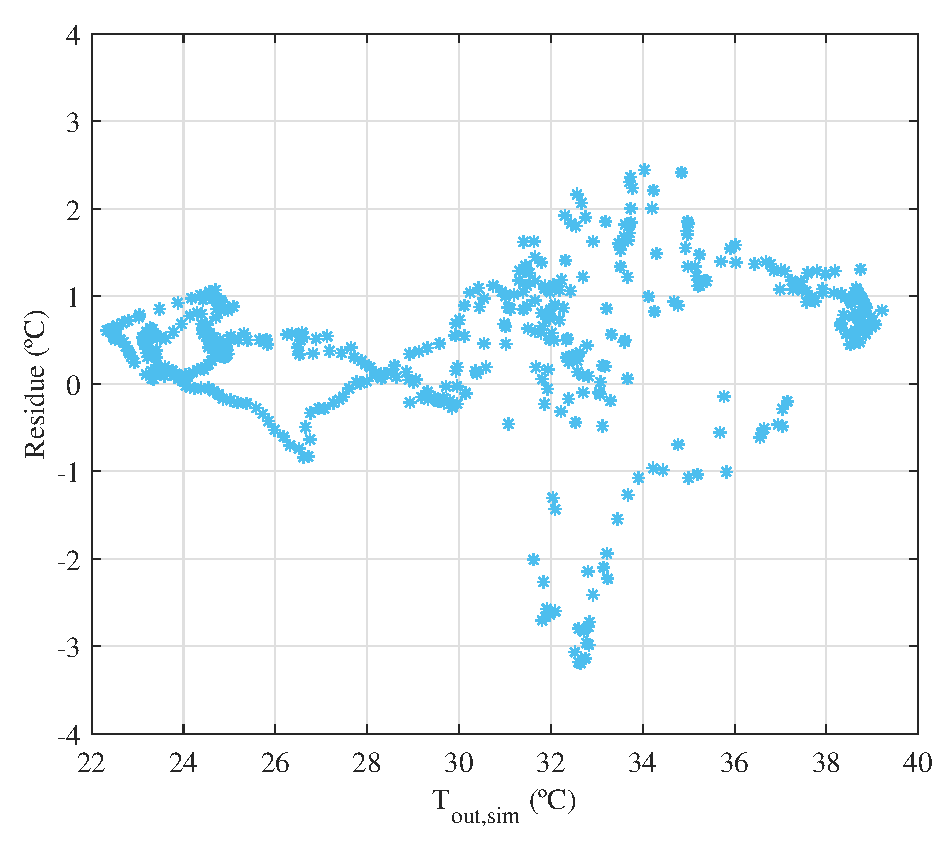
\includegraphics[scale=0.5,width=1.0\columnwidth]{figs/009-residue-5.eps}
		\subcaption{Residue vs. simulated $\rm{T_{out}}$.}
		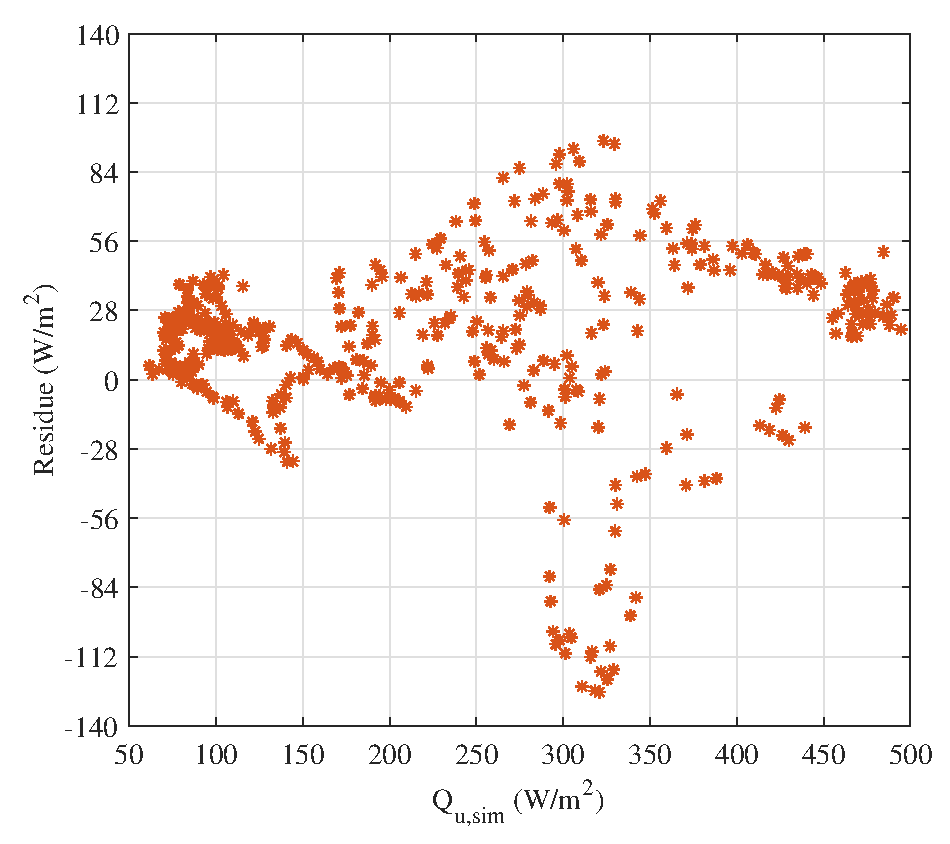
\includegraphics[scale=0.5,width=1.0\columnwidth]{figs/009-residue-6.eps}
		\subcaption{Residue vs. simulated $\rm{Q_{u}}$.}
	\end{minipage}
	
	\caption{Experimental and simulated results from 31$^{\rm{st}}$ May at 0.09 kg/(s m$^2$).}
	\label{009-3}
\end{figure}

%\Figure[scale=0.63,placement=!ht,label={009-3},caption={Experimental and simulated results from 31$^{\rm{st}}$ May at 0.09 kg/m$^2$.s. MAE is 4.9\% in terms of $\rm{T_{out}}$ and 27.5\% in terms of $\rm{Q_u}$.}]{figs/009-3.eps}

\subsubsection{Validation of results at high airflow rate}

Figure \ref{0115-3}(a) shows the graphs of solar radiation data, experimental and simulated results of the test on 28$^{\rm{th}}$ June ($\rm{G_{air}}$ = 0.115 kg/(s m$^2$), whereas Figures \ref{0115-3}(b) and \ref{0115-3}(c) present the residue plot in relation to the simulated values. On this clear sky day the calculated MAE for $\rm{T_{out}}$ and $\rm{Q_{u}}$ are 1.1\% and 7.0\%, respectively. In this case, the model underestimated 78\% of the predictions, where 83\% of the residues are between $\pm$0.6 $^{\rm{o}}$C and 83\% are between $\pm$30 W/m$^2$. After 14:00 the model mostly underestimated $\rm{Q_{u}}$ by 20 to 40 W/m$^2$. It is also noticed that the maximum residue is less than 1.0 $^{\rm{o}}$C and less than 40 W/m$^2$.

\begin{figure}[ht!]
\begin{minipage}{0.60\columnwidth}
		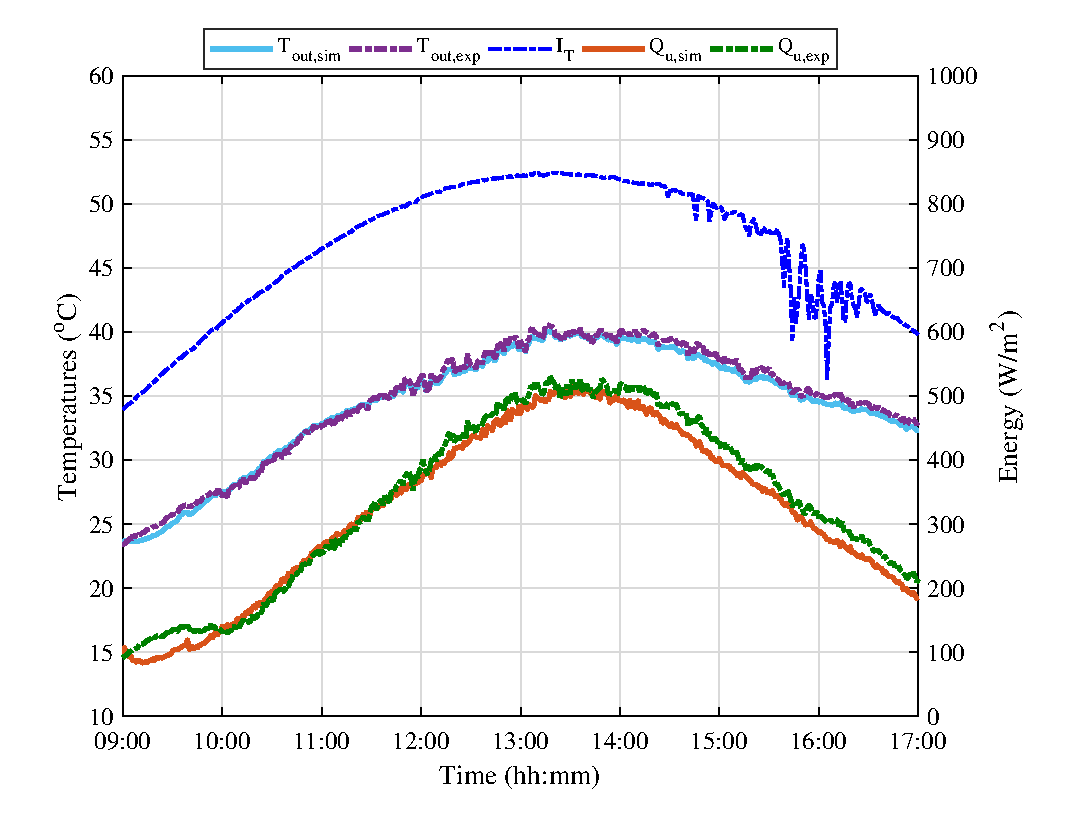
\includegraphics[width=0.99\columnwidth,height=65mm]{figs/0115-3.eps}
		%\\[-9mm]
		\subcaption{Experimental and simulated results over time.}
	\end{minipage}
	\begin{minipage}{0.39\columnwidth}
		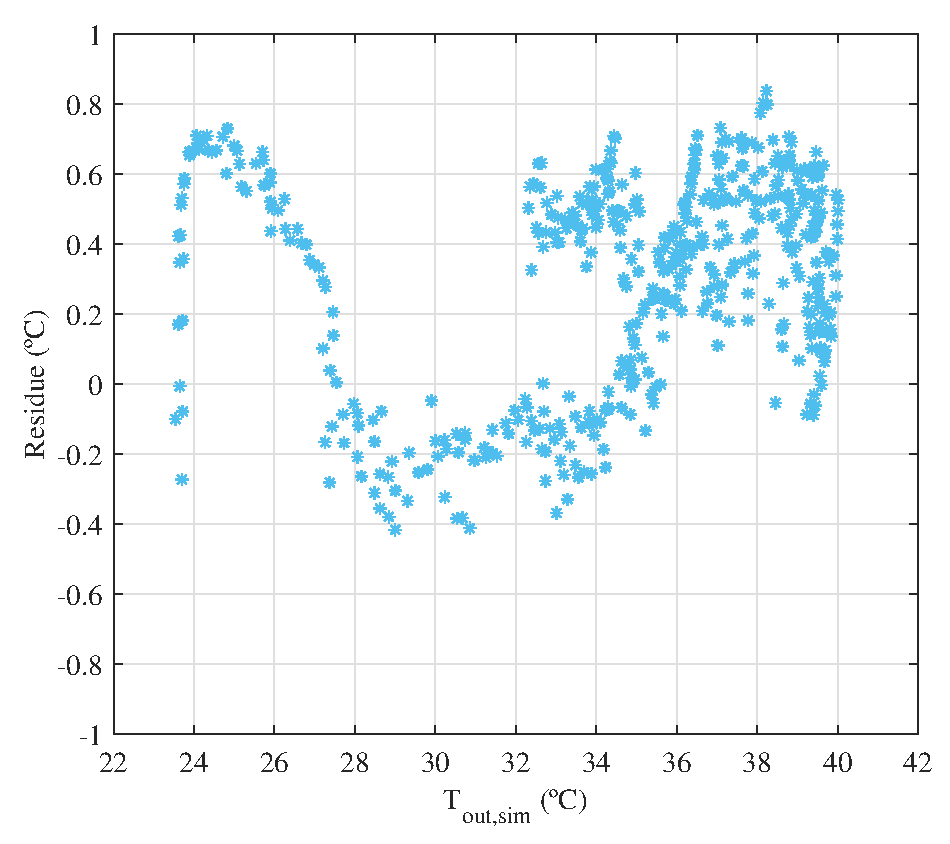
\includegraphics[scale=0.5,width=1.0\columnwidth]{figs/0115-residue-5.eps}
		\subcaption{Residue vs. simulated $\rm{T_{out}}$.}
		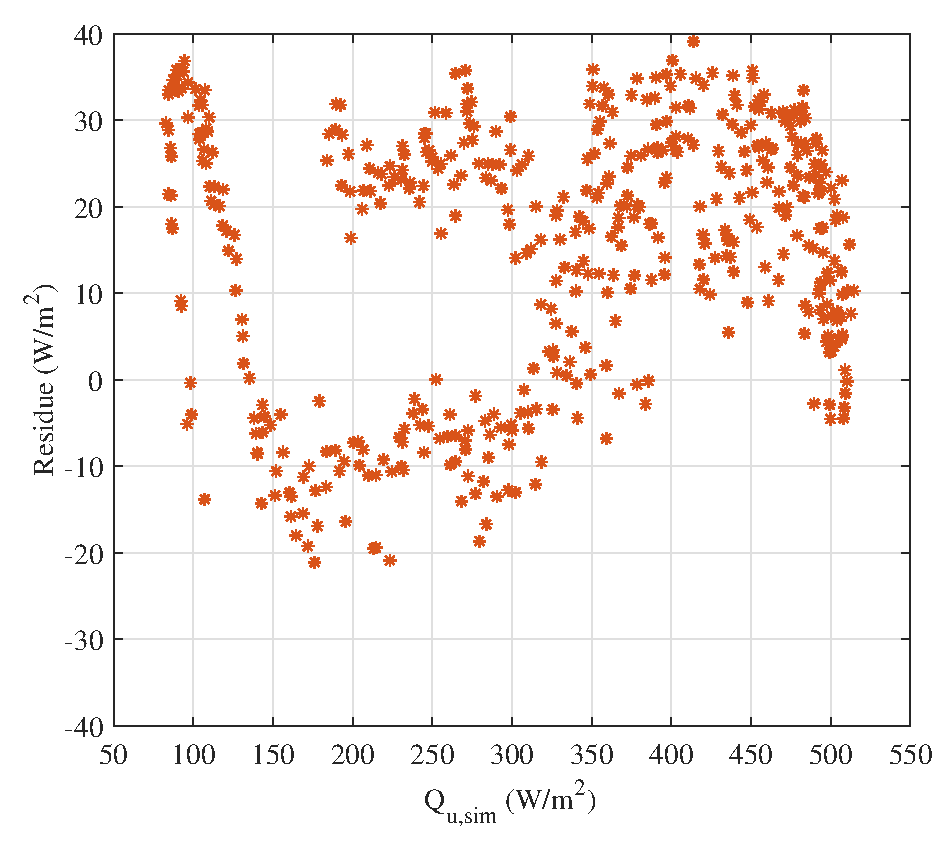
\includegraphics[scale=0.5,width=1.0\columnwidth]{figs/0115-residue-6.eps}
		\subcaption{Residue vs. simulated $\rm{Q_{u}}$.}
	\end{minipage}
	
	\caption{(a) Experimental and simulated results, (b) residues of $\rm{T_{out}}$, and (c) residues of $\rm{Q_{u}}$ from 28$^{\rm{th}}$ June at 0.115 kg/(s m$^2$).}
	\label{0115-3}
\end{figure}

%\Figure[scale=0.63,placement=!ht,label={0115-3},caption={Experimental and simulated results from 28$^{\rm{th}}$ June at 0.115 kg/m$^2$.s. MAE is 2.2\% in terms of $\rm{T_{out}}$ and 14\% in terms of $\rm{Q_u}$.}]{figs/0115-3.eps}

Hence, from the calculated MAE and residue plots, there was no effect of the airflow rate and time of operation on the model prediction. To check if solar radiation has influence on the model prediction, all residues were plotted against $\rm{I_{\!_T}}$ and shown in Figure \ref{res_it}. It can be seen that the residues are concentrated on the region of $\rm{I_{\!_T}}$ above 600 W/m$^2$ and most of them are between $\pm$2.0 $^{\rm{o}}$C and $\pm$50 W/m$^2$. The highest residues were observed for days with high intermittent clouds.

\begin{figure}[ht!]
	\begin{minipage}{0.49\columnwidth}
		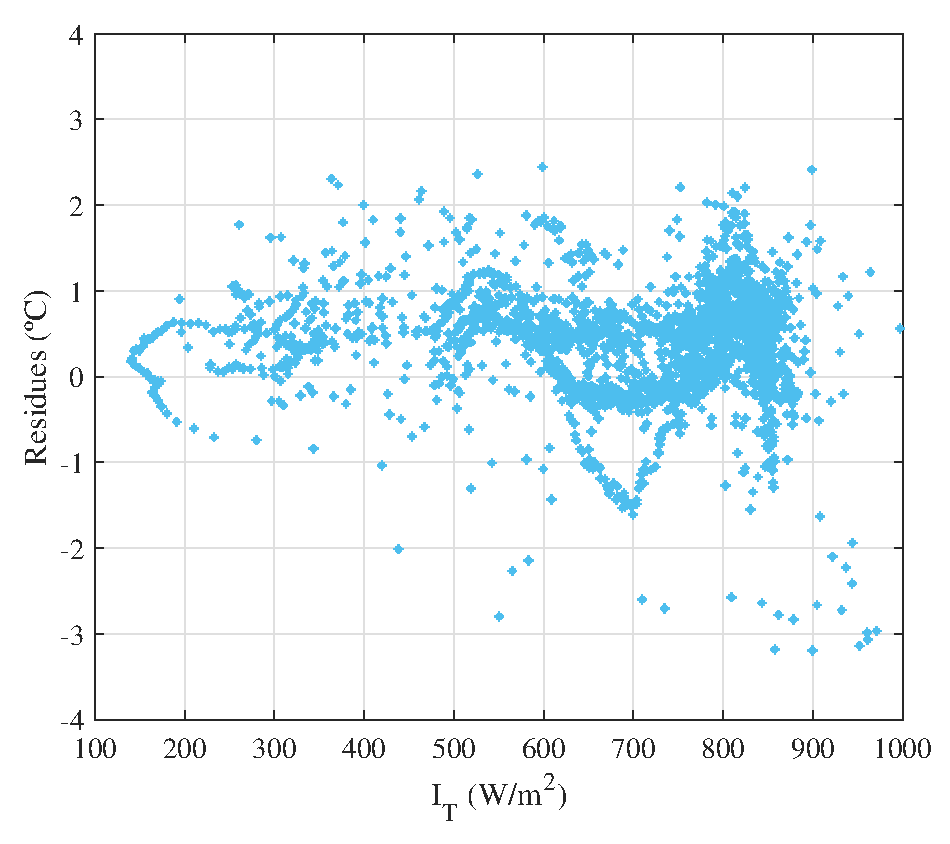
\includegraphics[width=0.95\columnwidth,height=5.5cm]{figs/residueT_it.eps}
		\subcaption{Residue vs. solar radiation for $\rm{T_{out}}$.}
	\end{minipage}
	\begin{minipage}{0.49\columnwidth}
		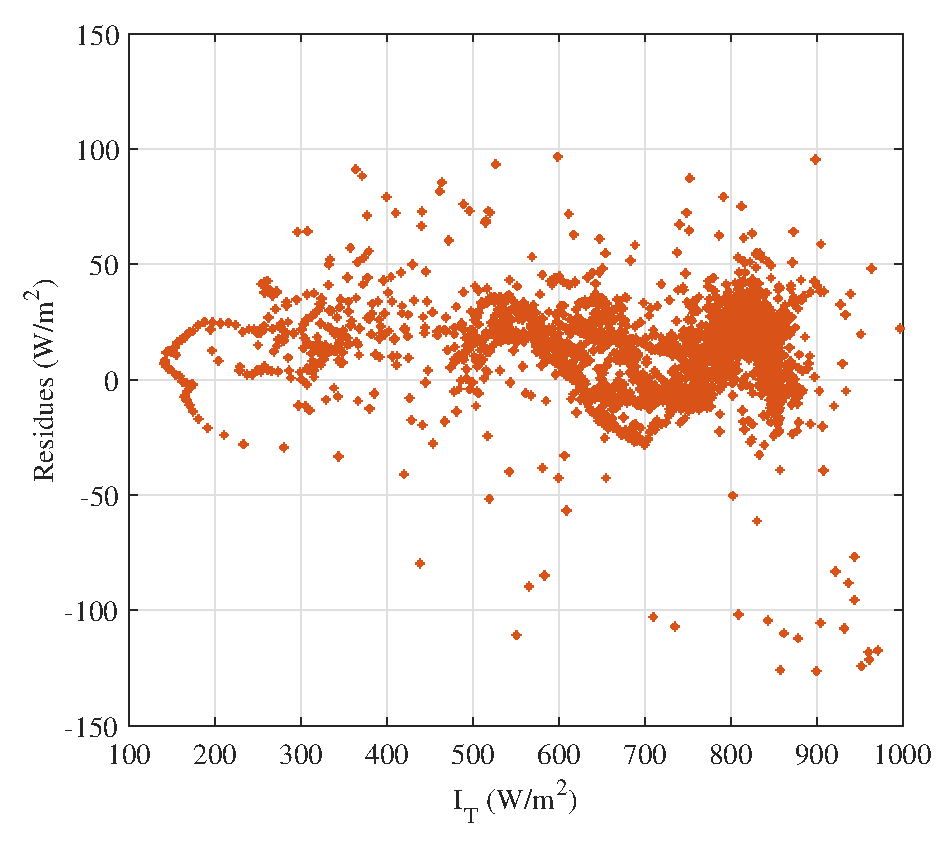
\includegraphics[width=1.0\columnwidth,height=5.5cm]{figs/residueQ_it.eps}
		\subcaption{Residue vs. solar radiation for $\rm{Q_u}$.}
	\end{minipage}
	\caption{Residues vs. solar radiation for (a) $\rm{T_{out}}$, and (b) $\rm{Q_u}$.}
	\label{res_it}
\end{figure}

Another way to analyse these residue data is by plotting the cumulative frequency distribution of each simulated output, as shown in Figure \ref{cdf}. From the cumulative distributions, 95\% of the data predicted have residues between $\pm$2 $^{\rm{o}}$C and $\pm$50 W/m$^{2}$C. It was also found that 65\% of the predictions are underestimated, which highlights the underestimation of the simulation results at most of the time.

\begin{figure}[ht!]
	\begin{minipage}{0.49\columnwidth}
		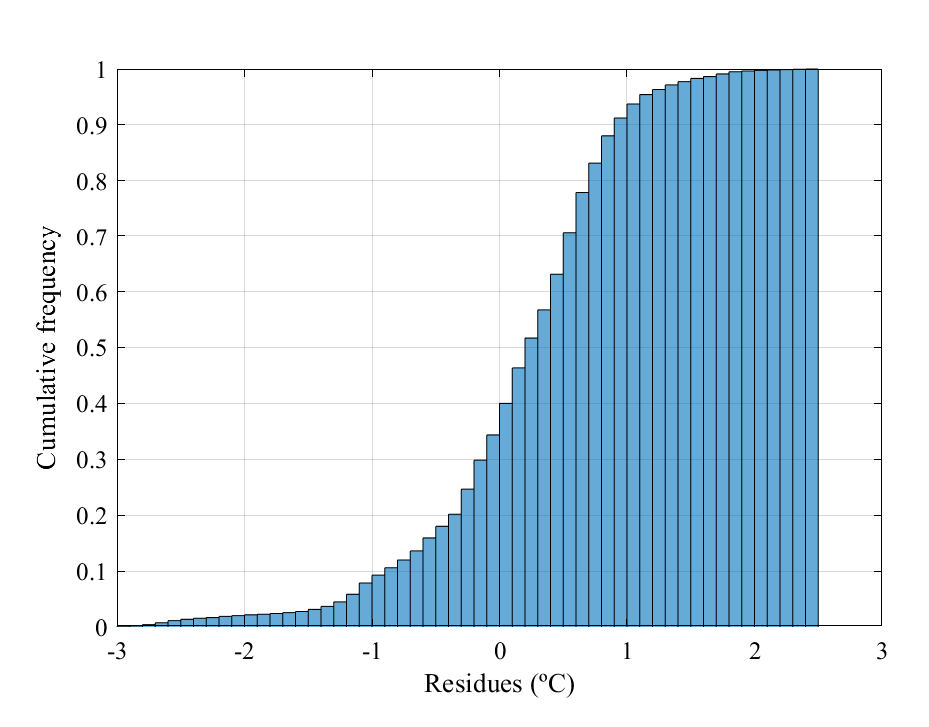
\includegraphics[width=0.95\columnwidth,height=5.5cm]{figs/cdf_T.eps}
		\subcaption{Cumulative frequency of residues from $\rm{T_{out}}$.}
	\end{minipage}
	\begin{minipage}{0.49\columnwidth}
		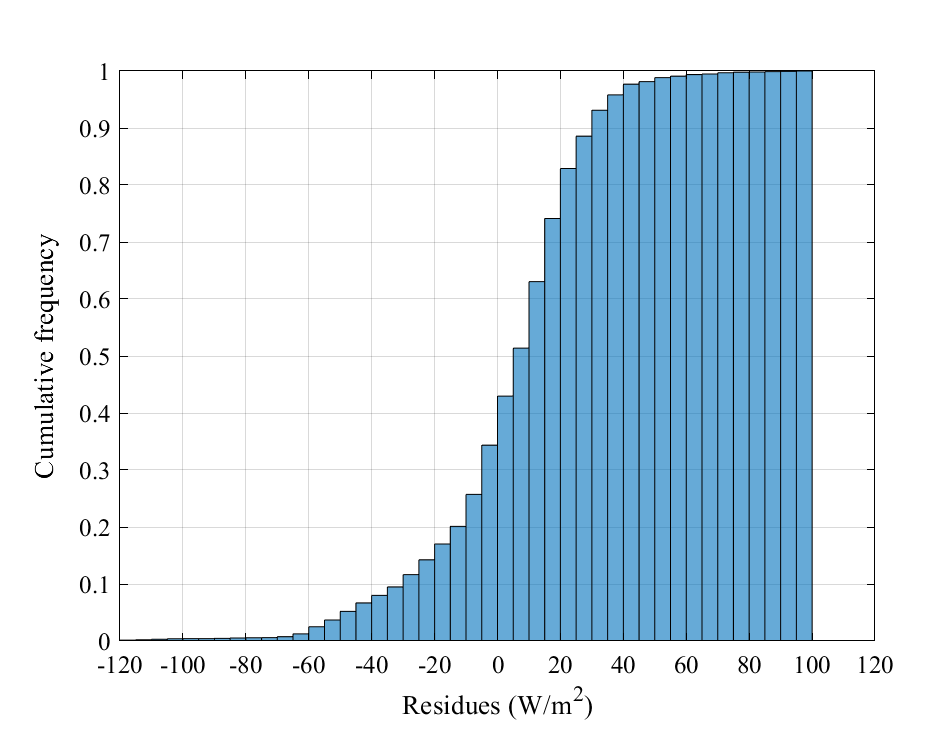
\includegraphics[width=1.0\columnwidth,height=5.5cm]{figs/cdf_Q.eps}
		\subcaption{Cumulative frequency of residues from $\rm{Q_u}$.}
	\end{minipage}
	\caption{Residual cumulative frequency distribution of (a) $\rm{T_{out}}$, and (b) $\rm{Q_u}$.}
	\label{cdf}
\end{figure}


\section{Thermal characterisation from simulation results}

After validation, the heat transfer model was used to characterise the system's thermal performance under the conditions of clear sky days at transient state. The inputs ranges, of which this system can be modelled, are depicted as follows:

\begin{description}
	\item[Solar radiation:] 500 -- 1000 W/m$^2$, where the lowest limit corresponds to the airflow temperature increase at the beginning of the operation;
	\item[Mass airflow rate:] 0.04 -- 0.12 kg/(s m$^2$), where the limits are coincident to the ones of the tests;
	\item[Ambient temperature:] 20 -- 30 $^{\rm{o}}$C, which includes all the measured data on clear sky days;
	\item[Wind speed:] 0 -- 10 m/s, to include all the data taken from Met Eireann website.
\end{description}

%In the first scenario,

%The parameters $\rm{T_{amb}}$, $\rm{v_w}$ and $\rm{I_{\!_T}}$ were kept constant during the simulations regardless the amount of beam and diffuse components, which allows to assume that $\gamma = $1.





%\begin{table}[!ht]
%	\caption{Input values for simulation}
%	\centering
%	\begin{tabular}{p{5.1cm}p{3.7cm}}
%		\hline \\[-10pt] 
%		\rule[-1ex]{0pt}{2.5ex} Model Input & Value/Range \\ [3pt]
%		\hline \\[-10pt]
%		\rule[-1ex]{0pt}{2.5ex} Total solar radiation ($\rm{I_{\!_T}}$) & 500 -- 1000 W/m$^2$ \\ [5pt]
%		\rule[-1ex]{0pt}{2.5ex} Ambient temperature ($\rm{T_{amb}}$) & 20 -- 30 $\rm{^o}$C \\ [5pt] 
%		\rule[-1ex]{0pt}{2.5ex} Wind speed ($\rm{v_w}$) & 0 -- 10 m/s \\ [5pt]
%		\rule[-1ex]{0pt}{2.5ex} Inlet air temperature ($\rm{T_{in}}$) & 20 -- 30 $\rm{^o}$C  \\ [5pt]
%		\rule[-1ex]{0pt}{2.5ex} Airflow rate ($\rm{G_{air}}$) & 0.04 -- 0.12 kg/(m$^2$.s)  \\ [5pt]
%		%\rule[-1ex]{0pt}{2.5ex} Optical efficiency ($\eta_{\rm{o}}$) & Eq. (\ref{optHts}) \\ 
%		
%		\hline 
%	\end{tabular} 
%	\label{inputs}
%\end{table}

\subsection{Thermal performance of a single collector}

To characterise this air heating system with one concentrator, a particular clear sky day (30$^{\rm{th}}$ June) was taken to represent the results. The simulation was performed at the five different airflow rates and the correspondent graphs of $\rm{T_{out}}$ were plotted in Figure \ref{Touts_sim}. All the temperature profiles reached their maximum levels in the hour of highest solar radiation ($\rm{I_{\!_T}}$ = 860 W/m$^2$). 

\Figure[scale=0.69,placement=!ht,label={Touts_sim},caption={Simulated $\rm{T_{out}}$ at the five different airflow rates used in the tests, under conditions of 30$^{\rm{th}}$ June.}]{figs/series_1st.eps}

With the simulation data obtained, Figure \ref{Tout-IT-Gair} presents the surface and contour plot to fit the air temperature rise ($\Delta \rm{T}$) as function of the solar radiation and airflow rate. In overall, the air temperature rise is observed from $\rm{I_{\!_T}}$ above 500 W/m$^2$ and increases in a nearly linear was as more energy is coming into the system. The opposite effect is noticed as the airflow is increased because $\Delta \rm{T}$ is inversely proportional to $\rm{G_{air}}$. Temperature rises above 27 $^{\rm{o}}$C can be obtained at airflow rate of 0.04 kg/(s m$^2$) when $\rm{I_{\!_T}}$ is above \mbox{860 W/m$^2$}.

\begin{figure}[ht!]
	\begin{minipage}{0.49\columnwidth}
		\includegraphics[scale=0.49]{figs/Tout_x_GT_Gair.eps}
		\subcaption{Surface plot.}
	\end{minipage}
	\begin{minipage}{0.49\columnwidth}
		\includegraphics[scale=0.49]{figs/contour_dT.eps}
		\subcaption{Contour plot.}
	\end{minipage}
	\caption{(a) Surface and (b) contour plot of air temperature rise vs. solar radiation and airflow rate.}
	\label{Tout-IT-Gair}
\end{figure}

%\Figure[scale=0.60,placement=!ht,label={Tout-IT-Gair},caption={Surface plot of air temperature rise vs. solar radiation and airflow rate.}]{figs/Tout_x_GT_Gair.eps}

To express these results in terms of useful energy, Figure \ref{QU-Tout-Gair} shows surface and contour plot of this output against air temperature rise and airflow rate. $\rm{Q_u}$ increases as $\rm{G_{air}}$ and $\Delta \rm{T}$ become higher as it is directly proportional to both inputs. The temperature increases more at lower airflow rates but at the cost of delivering low useful energy rate, which highlights the trade-off between energy collected and outlet air temperature.

\begin{figure}[ht!]
	\begin{minipage}{0.49\columnwidth}
		\includegraphics[scale=0.48]{figs/QU_Tout_Gair.eps}
		\subcaption{Surface plot.}
	\end{minipage}
	\begin{minipage}{0.49\columnwidth}
		\includegraphics[scale=0.48]{figs/contour_Q.eps}
		\subcaption{Contour plot.}
	\end{minipage}
	\caption{(a) Surface and (b) contour plot of useful energy vs. air temperature rise and airflow rate.}
	\label{QU-Tout-Gair}
\end{figure}

%\Figure[scale=0.60,placement=!ht,label={QU-Tout-Gair},caption={Surface plot of useful energy rate vs. air temperature rise and airflow rates.}]{figs/QU_Tout_Gair.eps}

Figure \ref{ef_curve2} shows simulated data takes under the same conditions depicted in Chapter \ref{Cap:Exp} at nearly steady state. Comparing the parameters of the Hottel-Whillier-Bliss equation, $\rm{F_{\!_R}}\eta_{\rm{o}}$ and $\rm{ F_{\!_R}{U_{\!_L}}}$ calculated by the thermal model are 0.64 and -3.02, respectively, with relative difference of 2\% and 10\% in relation to the parameters of the experimental data. The coefficient of correlation  of the simulated curve is 0.9.

\Figure[scale=0.65,placement=!ht,label={ef_curve2},caption={Experimental and simulated thermal efficiency curves.}]{figs/ef_curve2.eps}

\subsection{Simulation of three connected collectors}

The thermal performance of three collectors that are interconnected was analysed with regard to their connection in series and parallel configurations. The reason for selecting three collectors in this simulation is due to their collective total aperture height of approximately 1 meter when stacked above one another on a wall.

\subsubsection{Connection in series}

Figure \ref{D-series} illustrates the frontal view drawing of the collectors arranged in series. In this configuration, the airflow enters the system through the labeled inlet duct and exits through the indicated outlet duct. The drawing indicates that the airflow leaving the first collector (IACPC 1) immediately enters the second collector (IACPC 2) at its right end, while the airflow leaving IACPC 2 enters the third collector (IACPC 3) at its left end.

\Figure[scale=0.70,placement=!ht,label={D-series},caption={Frontal view of three collectors connected in series.}]{figs/Drawing-Series.png}

The outlet air temperature profiles at four different airflow levels throughout time of operation for the other two collectors are shown in Figure \ref{Temp-series}, where the results are for (a) the second collector and (b) for the third one.

\begin{figure}[ht!]
	\begin{minipage}{0.49\columnwidth}
		\includegraphics[scale=0.49]{figs/series_2nd.eps}
		\subcaption{Simulation results for the second collector.}
		
	\end{minipage}
	\begin{minipage}{0.49\columnwidth}
		\includegraphics[scale=0.49]{figs/series_3rd.eps}
		\subcaption{Simulation results for the third collector.}
		
	\end{minipage}
	\caption{Simulated $\rm{T_{out}}$ at four different airflow rates, for connection in series.}
	\label{Temp-series}
\end{figure}

Figure \ref{series2} shows the useful heat and the mean air temperature at noon hour as function of the airflow rate leaving each collector. The maximum mean $\rm{T_{out}}$ of the system is 72 $^{\rm{o}}$C for the lowest level of $\rm{G_{air}}$. On the other hand, the highest $\rm{G_{air}}$ is able to collect the highest $\rm{Q_{u}}$ value of 21.5 MJ/m$^{\rm 2}$ in total and delivering a mean temperature at noon of 48 $^{\rm{o}}$C. It is important to mention that the highest airflow rate can deliver approximately the same outlet air temperature as the the system consisting of a standalone collector at the lowest airflow rate. However the three-collector system collects 3 times more useful heat.  

\Figure[scale=0.65,placement=!ht,label={series2},caption={Total useful heat and mean $\rm{T_{out}}$ as function os the airflow rate level for connection in series.}]{figs/Qu-Tout-Gair-series.eps}

\subsubsection{Connection in parallel}

In Figure \ref{D-parallel} is shown the drawing of the collectors in frontal view connected in series, where the airflow is fed through the duct labelled as inlet. The main airflow is split into three equal airflows, each one coming into each collector on the left end. After leaving them on the right end, the small airflows are gathered and leave the system by the outlet duct.

\Figure[scale=0.70,placement=!ht,label={D-parallel},caption={Frontal view of three collectors connected in parallel.}]{figs/D-Parallel.png}

In Figure \ref{parallel1} is shown the graph of useful heat and outlet air temperature versus airflow rate for connection in parallel. In this case there is no increase in $\rm{T_{out}}$ but only for energy collection. This is the reason why the $\rm{T_{out}}$ graph is the profile leaving the first collector from Figure \ref{series2}. However the useful heat collection was found to be higher than for the system in series if the same level of $\rm{G_{air}}$ is considered. For instance, at $\rm{G_{air}}$ = 0.12 kg/(m$^{\rm 2}$.s), $\rm{Q_{u}}$ = 22.5 MJ/m$^{\rm 2}$. This type of connection is useful if the operator needs to deliver more thermal energy with a considerable increase in $\rm{T_{out}}$.

\Figure[scale=0.65,placement=!ht,label={parallel1},caption={Total useful heat and mean $\rm{T_{out}}$ as function os the airflow rate level for connection in parallel.}]{figs/Qu-Tout-Gair-parallel.eps}

%\subsubsection{Connection in series/parallel}

%\Figure[scale=0.70,placement=!ht,label={D-combo1-23},caption={Frontal view of three collectors connected in series/parallel mode 1.}]{figs/D-Combo1-23.png}

%\Figure[scale=0.70,placement=!ht,label={D-combo12-3},caption={Frontal view of three collectors connected in series/parallel mode 2.}]{figs/D-Combo12-3.png}

%\section{CFD modelling and simulation}
%
%Computational fluid dynamics or CFD is the analysis of systems involving fluid flow, heat and mass transfer by means of computer-based simulation. The technique is very powerful and spans a wide range of industrial and non-industrial application areas. The availability of affordable high-performance computing hardware and the introduction of user-friendly interfaces have led to a recent upsurge of interest, and CFD has entered into the wider industrial community since the 1990s. There are several unique advantages of CFD over experiment-based approaches to fluid systems design:
%
%\begin{itemize}
%    \item substantial reduction of lead times and costs of new designs;
%    \item ability to study systems where controlled experiments are difficult or impossible to perform (e.g., very large systems);
%    \item ability to study systems under hazardous conditions at and beyond their normal performance limits (e.g., safety studies and accident scenarios);
%    \item practically unlimited level of detail of results.
%\end{itemize}
%
%The equations governing the fluid flow are the continuity (conservation of mass), the Navier-Stokes (balance of momentum), and the energy (conservation of energy) equations. These equations form a system of coupled non-linear partial differential equations (PDEs). Due to the coupled nature of the equations and the presence of non-linear terms, the fluid flow equations are not trivial to be solved by analytical methods. Closed form analytical solutions are possible only if these PDEs can be made linear, either because non-linear terms naturally drop out or because the non-linear terms are  neglected compared to others. If the non-linearities in the governing PDEs cannot be neglected, which is often the case for most engineering flows, numerical methods need to be used to obtain solutions(\cite{Yadav2013}).

%CFD is the art of replacing the differential equations governing the Fluid Flow, with a set of algebraic equations (this process is called the discretization), which in turn can be solved with the aid of a digital computer to get an approximate solution. The commonly used discretization methods in CFD analysis are the finite difference method (FDM), the finite volume method (FVM), the finite element method (FEM), and the boundary element method (BEM). Some special cases of flow problems can also be solved using nonstandard method like, boundary integral methods, spectral methods, and pseudo-spectral methods. From the 1960s the aerospace industry has integrated CFD techniques into the design, R&D and manufacture of aircraft and jet engines.

%Increasingly CFD is becoming a vital component in the design of industrial products and processes. The ultimate aim of developments in the CFD field is to provide a capability comparable with other CAE (computer-aided engineering) tools such as stress analysis codes. The main reason why CFD has lagged behind is the tremendous complexity of the underlying behaviour, which precludes a description of fluid flows that is at the same time economical and sufficiently complete. The availability of affordable high-performance computing hardware and the introduction of user-friendly interfaces have led to a recent upsurge of interest, and CFD has entered into the wider industrial community since the 1990s. There are several unique advantages of CFD over experiment-based approaches to fluid systems design:

\section{Case study: barley drying}

%Barley is a versatile crop that finds application in the production of malted goods, flour or flakes for bakery products, formulation of dietary products, and animal feed. Around 90\% of barley is utilized for malting due to its sturdy grain texture, the presence of a protective hull during germination, and the long-standing tradition in brewing (Food Agricultural Organization of the United Nations, 2014).

Drying is a thermal process involving the evaporation of moisture from grains in order to maintain 
their quality during storage and prevent the proliferation of bacteria, fungi, and pests. Drying also enables farmers to produce higher quality products that are suitable for both personal consumption and commercial purposes. For cereal grain, the recommended safe moisture content is typically within the range of 13 -- 16\% on a dry basis. Heated air is employed to dry, being the most common means of heat transfer. As a result of the heat application, a concentration gradient is established, creating a vapour pressure differential that causes moisture to move from the interior of the kernel towards the surface; the moisture is then evaporated and carried away from the product by the circulating air (\cite{Bala2017}).

Barley is a versatile crop used for the production of malted products, flour, flakes for bakery, dietary formulations, and animal feed. The majority of barley production, approximately 90\%, is intended for malting purposes due to the grain's firm texture, the presence of a protective hull during the germination process, and traditional use in brewing. The malting process involves hydration, germination, and drying, which convert the starch and protein in barley seeds into amino acids and fermentable carbohydrates. These components are utilized by yeast during the fermentation process and contribute to the sensory characteristics of the malt. It is essential that the metabolic activity and germination index of barley are preserved following processing, drying, and storage to facilitate effective germination (\cite{Soares2016}).

In order to dry barley for malting, it is advised to maintain the maximum temperature in the grains at 45 $^{\rm{o}}$C, which can typically be achieved by using inlet air temperatures of approximately 60 -- 65 $^{\rm{o}}$C (\cite{Embrapa2021}; \cite{Syngenta2020}). These temperature parameters are crucial to achieve proper drying of barley grains without harming their cell structure, which in turn preserves their ability to germinate successfully. (\cite{Soares2016}).

Mathematical models can be employed to describe the process of drying. The thermal energy demand to dry a certain mass of product $\rm{M_{bar}}$ is described by Eq. (\ref{heat-duty}) (\cite{McCabe1993}):

\vspace{-0.75cm}
\begin{equation}
	\mathrm{Q_{dryer} = M_{bar}}\left[
	\begin{array}{l} 
		\mathrm{C_{p,bar}(T_{bar,out} - T_{bar,in}) + X_{in}C_{p,wl}(T_v - T_{bar,in}) + (X_{in} - X_{out})\lambda_v } \\
		\mathrm{+ X_{out}C_{p,wl}(T_{bar,out} - T_v) + (X_{in} - X_{out})C_{p,v}(T_{bar,out} - T_v)   }
	\end{array} \right]
	\label{heat-duty}
\end{equation}

\noindent where it takes into account: i) the initial and final barley's moisture content $\rm{X_{in}}$ and $\rm{X_{out}}$; ii) the initial barley temperature $\rm{T_{bar,in}}$; iii) the air temperature at the dryer's inlet; iv) implicitly, the air humidity, and; v) specific heat of barley, liquid and vapour water, and latent heat of vaporization. The inlet air temperature at the dryer is the outlet temperature at the solar heating system $\rm{T_{out}}$. The estimation of the temperature of vaporization $\rm{T_v}$ considers the ambient relative humidity and ambient temperature, and can be found using a numerical algorithm.

This energy demand is provided by an airflow pre-heated by gas burner, electric resistance or, partially, by solar air heaters to offset any other source of heating. Therefore, this topic aims at simulating the use of the solar air heating system previously validated to provide heated air to partially meet the energy required to dry barley. The assumptions for the simulation are depicted as follows:

%\Figure[scale=0.65,placement=!ht,label={auxiliary},caption={Schematic drawing of main heating system and auxiliary system for air heating.}]{figs/auxiliary.png}

\begin{itemize}
	\item Initial moisture content of barley is 20\% to be dried until it reaches 15\%;
	\item The source of heating is obtained by burning natural gas whose calorific value is 40 MJ/m$^{\rm{3}}$ (\cite{GOVUK2022});
	%\item 3 liters of natural gas is needed to dry 1 ton of barley by 1\% of moisture content;
	\item The airflow temperature set to dry barley is 60 $^{\rm{o}}$C so that it speeds up the drying process while it does not hinge metabolic activity;
	\item The dryer is adiabatic.
\end{itemize}

The present topic considered three scenarios: 
\begin{enumerate}
	\item Simulating only a gas burner to heat the airflow up to 60 $^{\rm{o}}$C to meet the energy demand;
	\item Simulating the solar heating system and a gas burner to heat the airflow up to 60 $^{\rm{o}}$C to meet the energy demand;
	\item Simulating only the solar heating system to heat the airflow with no air temperature limit to meet the energy demand.
\end{enumerate}

% Figure \ref{diagram-dry} shows the block diagram of the drying operation simulated in this topic. The whole system includes heating by the solar air heating system (SAHS), gas burner, a control system and a barley dryer. The control system is used to manipulate airflow rate to keep the airflow temperature lower or equal 60 $^{\rm{o}}$C. In case the temperature is lower, the valve is manipulated to allow natural gas (NG) to be fed into the gas burner to the airflow to reach 60 $^{\rm{o}}$C. In scenario 1, the SAHS is turned off hence the fresh air is entering the gas burner directly. In scenario 2, both SAHS and gas burner work together. Lastly, in scenario 3 the valve is closed off so that the fresh air is exclusively heated by the SAHS.

Figure \ref{diagram-dry} illustrates the schematic diagram of the drying process discussed in this study. The system comprises several key components: the Solar Air Heating System (SAHS), a gas burner, a control system, and a barley dryer. The role of the control system is to regulate the airflow rate, maintaining the airflow temperature at or below 60 $^{\rm{o}}$C. When this temperature falls below that threshold, the valve adjusts to introduce natural gas (NG) into the gas burner, raising the airflow temperature to 60 $^{\rm{o}}$C. In Scenario 1, the SAHS is inactive, allowing ambient air to enter the gas burner directly. In Scenario 2, both the SAHS and the gas burner operate simultaneously. Finally, in Scenario 3, the valve is closed, relying solely on the SAHS to heat the incoming fresh air.

\Figure[scale=0.74,placement=!ht,label={diagram-dry},caption={Block diagram of the simulated process of solar drying.}]{figs/system-drying.png}

All the scenarios considered the calculation of the barley mass dried and the amount of $\rm{CO_2}$ released to atmosphere by burning natural gas in 8h of operation to match the solar heating system working hours (9:00 to 17:00). The airflow rate levels used were the ones used previously in the model simulation. The solar radiation levels used was the real solar data presented in Figure \ref{Touts_sim} of 30$^{\rm{th}}$ June 2018 (clear sky day).

To illustrate in terms of energy, the SAHS is considered to be operating in series with the lowest and highest evaluated flow rates, as shown in Figures \ref{dry_1col}, \ref{dry_2col}, and \ref{dry_3col}. In these Figures, the red line represents the energy required for heated air to enter the dryer at 60 $^{\rm{o}}$C, while the blue line represents the energy supplied by the SAHS. In Figure \ref{dry_1col}, which represents the energy at the output of the first solar collector, for both flow rates, there is an energy deficit between the supplied and required energy, necessitating the activation of the gas burner to bridge this gap. In Figure \ref{dry_2col}, illustrating the energy at the output of the second collector, for the lowest airflow rate, there is a period of operation (between 12:20 and 14:30) where the energy from the SAHS surpasses the required energy, resulting in a surplus, and thus, the burner does not need to operate. Conversely, in Figure \ref{dry_3col}, at the output of the third collector, the period of surplus energy extends (between 11:30 and 15:00), requiring less from the burner. In the simulation with the highest airflow rate, the energy deficit naturally decreases.

\begin{figure}[ht!]
	\begin{minipage}{0.50\columnwidth}
		\includegraphics[scale=0.45]{figs/dry_low_1col.eps}
		\subcaption{Energy results at $\rm{G_{air}}$ = 26.10 kg/h.}
		
	\end{minipage}
	\begin{minipage}{0.50\columnwidth}
		\includegraphics[scale=0.45]{figs/dry_high_1col.eps}
		\subcaption{Energy results at $\rm{G_{air}}$ = 78.30 kg/h.}
		
	\end{minipage}
	\caption{Simulated energies for two different airflow rates at the first collector in series.}
	\label{dry_1col}
\end{figure}


\begin{figure}[ht!]
	\begin{minipage}{0.50\columnwidth}
		\includegraphics[scale=0.45]{figs/dry_low_2col.eps}
		\subcaption{Energy results at $\rm{G_{air}}$ = 26.10 kg/h.}
		
	\end{minipage}
	\begin{minipage}{0.50\columnwidth}
		\includegraphics[scale=0.45]{figs/dry_high_2col.eps}
		\subcaption{Energy results at $\rm{G_{air}}$ = 78.30 kg/h.}
		
	\end{minipage}
	\caption{Simulated energies for two different airflow rates at the second collector in series.}
	\label{dry_2col}
\end{figure}


\begin{figure}[ht!]
	\begin{minipage}{0.50\columnwidth}
		\includegraphics[scale=0.45]{figs/dry_low_3col.eps}
		\subcaption{Energy results at $\rm{G_{air}}$ = 26.10 kg/h.}
		
	\end{minipage}
	\begin{minipage}{0.50\columnwidth}
		\includegraphics[scale=0.45]{figs/dry_high_3col.eps}
		\subcaption{Energy results at $\rm{G_{air}}$ = 78.30 kg/h.}
		
	\end{minipage}
	\caption{Simulated energies for two different airflow rates at the third collector in series.}
	\label{dry_3col}
\end{figure}

\subsection{Scenario 1 -- Air heating by gas burner alone}

The required heat rate transferred to the airflow by the gas burner is calculated by Eq. (\ref{usefulenergy}). At an average ambient temperature of 25 $^{\rm{o}}$C and average relative humidity of 55\% on a clear sky day, the energy demand $\rm{Q_{dryer}}$ calculated is 0.05 kWh/kg of dried barley. Table \ref{gas-only} shows the values of energy required, mass dried, volume of natural gas burned and mass of $\rm{CO_2}$ released for each airflow level.

\begin{table}[h]
	\caption{Quantity of barley dried and amount of $\rm{CO_2}$ released for 8h of operation as function of the airflow rate only using gas burner for air heating.}
	\centering
	
	\begin{tabular}{ccccc}
		\hline \\ [-10pt]
		$\rm{G_{air}}$ (kg/h) & $\rm{Q_{req}}$ (kWh) & $\rm{M_{bar,dried}}$ (kg) & Gas volume (L) & $\rm{M_{CO2}}$ (kg) \\
		\hline \\ [-12pt]
		26.10 & 2.053 & 41 & 184.75 & 0.364 \\ [2pt]
		39.15 & 3.083 & 61 & 277.50 & 0.547 \\ [2pt]
		52.20 & 4.108 & 81 & 369.75 & 0.728 \\ [2pt]
		78.30 & 6.161 & 122 & 554.50 & 1.092 \\ 
		\hline
	\end{tabular}
	
	\label{gas-only}
\end{table}

At this airflow rate range and operating for 8 hours, 41 -- 122 kg of barley can be dried to reduce its moisture content from 20 to 15\% in dry basis.

\subsection{Scenario 2 -- Air heating using gas burner and solar system}

In this scenario, the energy required to heat the airflow to 60 $^{\rm{o}}$C is partially provided by the solar heating system and the complementary is by the gas burner. The connection between solar collectors in the system is also considered. Table \ref{gas-solar} shows the values for a connection of up to 3 collectors in series of energy required and energy provided by each mode, volume of natural gas burned, mass of $\rm{CO_2}$ released and the solar fraction for each airflow level. The solar fraction is defined as the ratio of the energy provided by the solar system ($\rm{Q_u}$) and the energy required ($\rm{Q_{req}}$). Additionally, Table \ref{gas-solar-parallel} shows values for a connection of 3 collectors operating in parallel, where the total airflow rates are triple the values for the range in series (78.30 -- 235 kg/h).


\begin{table}[h]
	\caption{Quantity of barley dried and amount of $\rm{CO_2}$ released for 8h of operation as function of the airflow rate using gas burner and solar system for air heating for connection of up to 3 collectors in series.}
	\centering
	
	\begin{tabular}{rrrrrrrr}
		\hline \\ [-10pt]
		 \makecell{$\rm{G_{air}}$ \\ (kg/h)} & \makecell{$\rm{Q_{req}}$ \\ (kWh)} & 	\makecell{$\rm{Q_{u}}$ \\ (kWh)} & 	\makecell{$\rm{Q_{burner}}$  \\ (kWh)} & \makecell{Gas Volume \\ (L)} & \makecell{$\rm{M_{CO2}}$  \\ (kg)} & \makecell{Solar \\ Fraction} \\
		\hline \\ [-10pt]
		\multicolumn{7}{c}{After the $\rm{1^{st}}$ collector} \\ \hline \\ [-10pt]
		26.10 & 2.053 & 0.933 & 1.119 & 100.75 & 0.198 & 0.4547 \\ [2pt]
		39.15 & 3.083 & 0.978 & 2.106 & 189.50 & 0.373 & 0.3171 \\ [2pt]
		52.20 & 4.108 & 1.000 & 3.108 & 279.75 & 0.551 & 0.2434 \\ [2pt]
		78.30 & 6.161 & 1.100 & 5.061 & 455.50 & 0.897 & 0.1785 \\
		\hline \\ [-10pt]
		\multicolumn{7}{c}{After the $\rm{2^{nd}}$ collector in series} \\ \hline \\ [-10pt]
		26.10 & 2.053 & 1.544 & 0.508 & 45.75 & 0.090 & 0.7524 \\ [2pt]
		39.15 & 3.083 & 1.635 & 1.448 & 130.31 & 0.257 & 0.5304 \\ [2pt]
		52.20 & 4.108 & 1.726 & 2.382 & 214.38 & 0.422 & 0.4202 \\ [2pt]
		78.30 & 6.161 & 1.908 & 4.253 & 382.75 & 0.754 & 0.3097 \\ 
		\hline \\ [-10pt]
		\multicolumn{7}{c}{After the $\rm{3^{rd}}$ collector in series} \\ \hline \\ [-10pt]
		26.10 & 2.053 & 1.819 & 0.233 & 21.00 & 0.041 & 0.7904 \\ [2pt]
		39.15 & 3.083 & 2.015 & 1.068 & 96.13 & 0.189 & 0.6850 \\ [2pt]
		52.20 & 4.108 & 2.211 & 1.897 & 170.75 & 0.336 & 0.5766 \\ [2pt]
		78.30 & 6.161 & 2.603 & 3.558 & 320.25 & 0.631 & 0.4225 \\
		\hline
	\end{tabular}
	
	\label{gas-solar}
\end{table}

The amount of barley dried is the same as shown in Table \ref{gas-only} because the air temperature is set to 60 $^{\rm{o}}$C to enter the dryer. For a connection of 3 collectors in series, this solar heating system can offset from 42 to 79\% of the energy provided by the gas burner alone. 

\begin{table}[h]
	\caption{Quantity of barley dried and amount of $\rm{CO_2}$ released for 8h of operation as function of the airflow rate using gas burner and solar system for air heating for connection of 3 collectors in parallel.}
	\centering
	
	\begin{tabular}{rrrrrrrr}
		\hline \\ [-10pt]
		\makecell{$\rm{G_{air}}$ \\ (kg/h)} & \makecell{$\rm{Q_{req}}$ \\ (kWh)} & 	\makecell{$\rm{Q_{u}}$ \\ (kWh)} & 	\makecell{$\rm{Q_{burner}}$  \\ (kWh)} & \makecell{Gas Volume \\ (L)} & \makecell{$\rm{M_{CO2}}$  \\ (kg)} & \makecell{Solar \\ Fraction} \\
		\hline \\ [-10pt]
		3x26.10 & 6.161 & 4.870 & 1.291 & 116.20 & 0.229 & 0.7904 \\ [2pt]
		3x39.15 & 9.250 & 6.336 & 2.914 & 262.55 & 0.517 & 0.6850 \\ [2pt]
		3x52.20 & 12.325 & 7.107 & 5.218 & 469.66 & 0.925 & 0.5766 \\ [2pt]
		3x78.30 & 18.483 & 7.810 & 10.673 & 960.60 & 1.892 & 0.4225 \\ 
		\hline
	\end{tabular}
	
	\label{gas-solar-parallel}
\end{table}

Considering collectors operating in parallel, the energy required is evidently increased due to higher airflow levels. The useful energy collected by the solar system is also higher. The solar fraction calculated is the same obtained when the system is operated in series, meaning that both connections will offset the the same energy levels relative to the required ones. The advantage of operating in parallel over in series is that the amount of barley dried is increased by 3 times: 122 -- 366 kg of barley can be dried to reduce its moisture content from 20 to 15\% in dry basis.




\subsection{Scenario 3 -- Air heating using solar system alone}

In this scenario, the energy transferred to the airflow is only provided by the solar collectors. For most of the time, the solar energy is insufficient to rise the temperature to 60 $^{\rm{o}}$C, which resulted in low drying rates, and therefore in lower dried mass of barley. Table \ref{solar-only} shows the mass of barley that can be dried if only the solar heating system is would be used in the operation. The quantity of mass dried varies from 22 -- 61 kg, considerably less compared to the other systems as the drying rate is lower. 

\begin{table}[h]
	\caption{Quantity of barley dried and amount of $\rm{CO_2}$ released for 8h of operation as function of the airflow rate using solar system alone for air heating for connection of 3 collectors in series.}
	\centering
	
	\begin{tabular}{cccccccc}
		\hline \\ [-10pt]
		\multirow{2}{*}{ $\rm{G_{air}}$  (kg/h)} & \multicolumn{2}{c}{After $\rm{1^{st}}$ collector} & \multicolumn{2}{c}{After $\rm{2^{nd}}$ collector} & \multicolumn{2}{c}{After $\rm{3^{rd}}$ collector} \\
		
		 & \makecell{$\rm{Q_{u}}$ \\ (kWh)} & 	\makecell{$\rm{M_{bar,dried}}$ \\ (kg)} & 	\makecell{$\rm{Q_{u}}$  \\ (kWh)} & \makecell{$\rm{M_{bar,dried}}$ \\ (kg)} & \makecell{$\rm{Q_{u}}$  \\ (kWh)} & \makecell{$\rm{M_{bar,dried}}$ \\ (kg)} \\
		\hline \\ [-10pt]
		26.10 & 0.933 & 22 & 1.544 & 33 & 1.819 & 37 \\ [2pt]
		39.15 & 0.978 & 24 & 1.635 & 37 & 2.015 & 43 \\ [2pt]
		52.20 & 1.000 & 25 & 1.726 & 40 & 2.211 & 50 \\ [2pt]
		78.30 & 1.100 & 28 & 1.908 & 47 & 2.603 & 61 \\ 
		\hline
	\end{tabular}
	
	\label{solar-only}
\end{table}

When the air heating collectors are connected in parallel, the thermal energy absorbed by the airflow rate is higher, which results in more mass dried, as shown in Table \ref{gas-only-parallel}. As the airflow rate is tripled, the quantity of barley dried is tripled as well (66 -- 84 kg), which is an advantage over the connection in series.

\begin{table}[h]
	\caption{Quantity of barley dried and amount of $\rm{CO_2}$ released for 8h of operation as function of the airflow rate using solar system alone for air heating for connection of 3 collectors in parallel.}
	\centering
	
	\begin{tabular}{ccc}
		\hline \\ [-10pt]
		$\rm{G_{air}}$ (kg/h) & $\rm{Q_{u}}$ (kWh) & $\rm{M_{bar,dried}}$ (kg) \\
		\hline \\ [-10pt]
		3x26.10 & 2.800 & 66 \\ [2pt]
		3x39.15 & 2.933 & 72 \\ [2pt]
		3x52.20 & 3.000 & 75 \\ [2pt]
		3x78.30 & 3.300 & 84 \\ 
		\hline
	\end{tabular}
	
	\label{gas-only-parallel}
\end{table}

%From the airflow range used in this research, one common level can be taken to compare the 3 scenarios treated previously, which is 78.3 kg/h. This comparison can be made considering mass of barley dried, volume of natural gas burnt and solar fraction, as shown in Table \ref{scenario-comparison}.  The data suggests that the use of solar air heating systems can significantly reduce the reliance on gas heating, with the gas burner + SAHS in parallel system having the lowest consumption of gas and highest solar fraction of all the systems listed. However, the choice of heating system will depend on various factors, including the availability of sunlight, the cost and availability of natural gas.

In this study, a particular airflow range was utilized, and a common level of 78.3 kg/h can be used to compare the three previously analyzed scenarios. This assessment can be conducted by examining the mass of dried barley, the amount of natural gas burned, and the solar fraction, all of which are presented in Table \ref{scenario-comparison}.  The gas burner system has the highest gas volume consumption of 554.5 L and a solar fraction of 0, meaning it relies completely on gas for heating. On the other hand, the SAHS standalone system produces less dried mass, but both connections have a solar fraction of 1, indicating that they rely solely on solar energy. The results indicate that the use of solar air heating systems can substantially reduce dependence on natural gas heating. Specifically, the gas burner + SAHS in parallel configuration exhibited the lowest gas consumption and highest solar fraction among all the listed systems with gas burner. Nevertheless, the selection of a heating system will depend on various factors, such as sunlight availability, natural gas cost, and accessibility.

\begin{table}[h]
	\caption{Comparison of the 3 scenarios at $\rm{G_{air}}$ = 78.3 kg/h for 8h of operation. }
	\centering
	
	\begin{tabular}{lrrr}
		\hline \\ [-10pt]
		Type of system & $\rm{M_{bar,dried}}$ (kg) & Gas volume (L) & Solar fraction \\
		\hline \\ [-10pt]
		Gas burner only & 122 & 554.50 & 0.00 \\ [2pt]
		Gas burner + SAHS series & 122 & 320.25 & 0.42 \\ [2pt]
		Gas burner + SAHS parallel & 122 & 116.20 & 0.79 \\ [2pt]
		SAHS series & 61 & 0.00 & 1.00 \\ [2pt] 
		SAHS parallel & 65 & 0.00 & 1.00 \\
		\hline
	\end{tabular}
	
	\label{scenario-comparison}
\end{table}

\section{Chapter Summary}

A thermal modelling and simulation of the proposed solar air heating system was developed and it was validated against experimental data. Results show that, in general, the heat transfer model underestimates 65\% of the data and 95\% of the residues generated are between $\pm$2 $^{\rm{o}}$C and $\pm$50 W/m$^2$. In overall, the mean absolute error in terms of temperature was found to be 2\% and in terms of useful energy was 8\%. After validation, the system has been characterised within a certain range of inputs.

The model was also used to simulate results at nearly steady state condition. The thermal efficiency curve was plotted and compare it to the experimental one. The parameters of the Hottel-Whillier-Bliss equation $\rm{F_{\!_R}}\eta_{\rm{o}}$ and $\rm{ F_{\!_R}{U_{\!_L}}}$ calculated by the thermal model are 0.64 and -3.02, with relative difference of 2\% and 10\%, respectively, in relation to the parameters of the experimental data.

The thermal modelling was also used to predict the thermal performance of three connected collectors in series and in parallel. The connection in series is able to deliver higher outlet airflow temperatures whereas the connection in parallel can collect more useful heat but delivering the same airflow temperature as if it is leaving the first collector in series.

Lastly, this model was used for simulating barley drying. Three scenarios were considered to meet the energy demand: simulating only a gas burner to heat the airflow up to 60 $^{\rm{o}}$C; simulating the solar heating system and a gas burner to heat the airflow up to 60 $^{\rm{o}}$C, and; simulating only the solar heating system to heat the airflow with no air temperature limit. From an specific airflow level used in the simulations, the gas burner system has the highest gas volume consumption and a solar fraction of 0, meaning it relies completely on gas for heating. On the other hand, the SAHS standalone system produces less dried mass, but both connections have a solar fraction of 1, indicating that they rely solely on solar energy. The results indicate that the use of solar air heating systems can substantially reduce dependence on natural gas heating. Specifically, the gas burner + SAHS in parallel configuration exhibited the lowest gas consumption and highest solar fraction among all the listed systems with gas burner. Nevertheless, the selection of a heating system will depend on various factors, such as sunlight availability, natural gas cost, and accessibility.





%A for abbreviations
\nomenclature[A]{ODE}{Ordinary Differential Equation}
\nomenclature[A]{CPC}{Compound Parabolic Concentrator}
\nomenclature[A]{CFD}{Computational Fluid Dynamics}
\nomenclature[A]{IACPC}{Inverted Absorber Compound Parabolic Concentrator}

%N for latin
\nomenclature[N]{$\rm{U}$}{Internal energy (J)}
\nomenclature[N]{$\rm{S}$}{Solar radiation rate absorbed (W)}
%\nomenclature[N]{$\rm{Q_{L,1}}$}{Heat loss rate from the absorber (W)}
%\nomenclature[N]{$\rm{Q_{L,2}}$}{Heat loss rate from the glazing (W)}
\nomenclature[N]{$\rm{Q_{u}}$}{Useful energy rate transferred to the airflow (W)}
\nomenclature[N]{$\rm{t}$}{Time (s)}
\nomenclature[N]{R}{Thermal resistance (K/W)}
\nomenclature[N]{h}{Heat transfer coefficient (W/(m$^2$K))}
\nomenclature[N]{$\rm{T}$}{Temperature (K)}
\nomenclature[N]{$\rm{M}$}{Mass (kg)}
\nomenclature[N]{$\rm{I_D}$}{Diffuse solar radiation (W/m$^2$)}
\nomenclature[N]{$\rm{I_B}$}{Beam solar radiation (W/m$^2$)}
\nomenclature[N]{$\rm{C}$}{Geometric concentration ratio}
\nomenclature[N]{$\rm{I_T}$}{Global solar radiation (W/m$^2$)}
\nomenclature[N]{$\rm{A}$}{Area (m$^2$)}
\nomenclature[N]{$\rm{L_{col}}$}{Collector length (m)}
%\nomenclature[N]{$\rm{\overline W_{glaz}}$}{Glazing characteristic length (m)}
%\nomenclature[N]{$\rm{T_c}$}{Temperature at the surroundings of the glazing (K)}
\nomenclature[N]{$\rm{Re}$}{Reynolds number}
\nomenclature[N]{$\rm{Ra}$}{Rayleigh number}
\nomenclature[N]{$\rm{Pr}$}{Prandtl number}
\nomenclature[N]{$\rm{W}$}{Width (m)}
\nomenclature[N]{$\rm{k_{air}}$}{Air thermal conductivity (W/m K)}
\nomenclature[N]{$\rm{C_{p}}$}{Specific heat (J/(kg K))}
\nomenclature[N]{$\rm{G_{air}}$}{Mass airflow rate based on the absorber area (kg/(s m$^2$))}
\nomenclature[N]{$\rm{A_{abs}^{'}}$}{Absorber area without the holes (m$^2$)}
\nomenclature[N]{$\rm{Nu}$}{Nusselt number}
\nomenclature[N]{$\rm{v}$}{Air velocity (m/s)}
\nomenclature[N]{$\rm{g}$}{Acceleration due to gravity (9.81 m/s$^2$)}
\nomenclature[N]{H}{Height (m)}
\nomenclature[N]{$\rm{U_L}$}{Overall heat loss coefficient (W/(m$^2$ K))}
\nomenclature[N]{$\rm{d_{air}}$}{Air density (kg/m$^3$)}
\nomenclature[N]{$\rm{N_{obs}}$}{Number of observations}
\nomenclature[N]{$\rm{X_{exp}}$}{Experimental or observed value of the variable X}
\nomenclature[N]{$\rm{X_{sim}}$}{Simulated of predicted value of the variable X}
%\nomenclature[N]{$\rm{MAE}$}{Mean absolute error}
\nomenclature[N]{$\rm{a_{s}}$}{Altitude solar angle}
\nomenclature[N]{$\rm{t_{ST}}$}{Solar time}
\nomenclature[N]{$\rm{t_{LST}}$}{Local standard time}
\nomenclature[N]{$\rm{E_{T}}$}{Equation of time}
\nomenclature[N]{$\rm{l_{ST}}$}{Standard longitude}
\nomenclature[N]{$\rm{l_{local}}$}{Local longitude}
\nomenclature[N]{$\rm{X_{in}}$}{Barley moisture content at the dryer's inlet (in dry base)}
\nomenclature[N]{$\rm{X_{out}}$}{Barley moisture content at the dryer's outlet (in dry base)}

%P for greek
\nomenclature[P]{$\rm{\ell}$}{Hole pitch (m)}
\nomenclature[P]{$\rm{\varphi_p}$}{Absorber porosity}
\nomenclature[P]{$\rm{\varphi_h}$}{Hole size (m)}
%\nomenclature[P]{$\rm{\Delta T_{m}}$}{Logarithmic mean difference temperature (K)}
\nomenclature[P]{$\Delta \rm{t}$}{Time step (s)}
\nomenclature[P]{$\nu_{\rm{air}}$}{Air kinematic viscosity (m$^2$/s)}
\nomenclature[P]{$\varepsilon_{\rm{eff}}$}{Effective emissivity}
\nomenclature[P]{$\varepsilon$}{Infra-red emissivity}
\nomenclature[P]{$\alpha$}{Absorptivity}
\nomenclature[P]{$\beta_{\rm{th}}$}{Volume expansion coefficient of the air (K$^{-1}$)}
\nomenclature[P]{$\sigma$}{Stefan-Boltzmann constant ($5.67$ \rm{x} ${10^{-8}}$ W/(m$^2$ K$^4$))}
\nomenclature[P]{$\eta_{\rm{th}}$}{Thermal efficiency}
\nomenclature[P]{$\eta_{\rm{o}}$}{Optical efficiency}
\nomenclature[P]{$\xi$}{Mean absolute error}
\nomenclature[P]{$\tau$}{Transmissivity}
\nomenclature[P]{$\gamma_{\rm{col}}$}{Collector's azimuth angle}
\nomenclature[P]{$\gamma_{\rm{s}}$}{Solar azimuth angle}

%S for subscripts
\nomenclature[S]{in}{Air at the inlet}
\nomenclature[S]{out}{Air at the outlet}
\nomenclature[S]{h}{Hole}
\nomenclature[S]{w}{Wind}
\nomenclature[S]{R1}{Radiation from absorber to glazing}
\nomenclature[S]{C1}{Convection from absorber to glazing}
\nomenclature[S]{R2}{Radiation from glazing to ambient}
\nomenclature[S]{C2}{Convection from glazing to ambient}
%\nomenclature[S]{C11}{Convection from absorber to bottom of tertiary section}
%\nomenclature[S]{C12}{Convection from bottom of tertiary section to glazing}
\nomenclature[S]{HX}{Convection from absorber to airflow}
\nomenclature[S]{abs}{Absorber}
\nomenclature[S]{glaz}{Glazing}
\nomenclature[S]{amb}{Ambient}
\nomenclature[S]{apt}{Aperture}
\nomenclature[S]{TS}{Tertiary section}
\nomenclature[S]{avg}{Average}
\nomenclature[S]{v}{Vaporization point}
\nomenclature[S]{bar}{Barley grains}


%constant solar radiation at various levels, ambient temperature and wind speed at the steady state condition, and; ii) solar radiation, ambient temperature and wind speed data under transient state. Table \ref{inputs} presents all the inputs values used in the simulation.

%In the first scenario,

%The parameters $\rm{T_{amb}}$, $\rm{v_w}$ and $\rm{I_{\!_T}}$ were kept constant during the simulations regardless the amount of beam and diffuse components, which allows to assume that $\gamma = $1. The constant values of $\rm{T_{amb}}$ and $\rm{v_w}$ used are averages over the period of operation (summertime). The effect of the tertiary section height ($\rm{H_{\!_{TS}}}$) was under investigation and the optical efficiency $\eta_{\rm{o}}$ assumed average values over the period of operation, only as a function of $\rm{H_{\!_{TS}}}$. Hence, the relationship between $\eta_{\rm{o}}$ and $\rm{H_{\!_{TS}}}$ is given by Eq. (\ref{optHts}):

%\begin{equation}
%\mathrm{\eta_o = 0.6801 - 0.2386H_{\!_{TS}} + 0.0492H_{\!_{TS}}^2}
%\label{optHts}
%\end{equation}

%\noindent which is a quadratic curve fit from the optical data obtained by the 3D ray tracing discussed in Chapter \ref{Cap:Opt}. %Table \ref{inputs} presents all the inputs values used in the simulation. The range of inputs selected is depicted as follows:

%%\begin{description}
%%	\item[Solar radiation:] range of 0 -- 1200 W/m$^2$, which corresponds from zero to high levels achievable in the summer;
%%	\item[Mass airflow rate:] from 0.04 to 0.11 kg/(m$^2$.s) to represent the values used in the experiments (Table \ref{GxV});
%%	\item[Tertiary section height:] 0 -- 0.29 m (or 0 -- 2$\rm{W_{abs}}$) to better understand the effect of this parameter.
%%\end{description}

%In the last scenario, solar and met data used are from 2014 measured at Kevin St roof. Therefore, the simulation steps must be ran once per day. Table \ref{inputs} presents all the inputs values used in the simulation. 

%Moreover, the data collection frequency is once a minute and then was interpolated to be used once a second throughout the period of analysis. 

%%\begin{table}[!ht]
%%	\caption{Input values for simulation}
%%	\centering
%%	\begin{tabular}{p{5.1cm}p{3.7cm}}
%%		\hline \\[-10pt] 
%%		\rule[-1ex]{0pt}{2.5ex} Model Input & Value/Range \\ [3pt]
%%		\hline \\[-10pt]
%%		\rule[-1ex]{0pt}{2.5ex} Total solar radiation ($\rm{I_{\!_T}}$) & 0 -- 1200 W/m$^2$ \\ [5pt]
%%		\rule[-1ex]{0pt}{2.5ex} Ambient temperature ($\rm{T_{amb}}$) & 23 $\rm{^o}$C \\ [5pt] 
%%		\rule[-1ex]{0pt}{2.5ex} Wind speed ($\rm{v_w}$) & 6 m/s \\ [5pt]
%%		\rule[-1ex]{0pt}{2.5ex} Tertiary section height ($\rm{H_{\!_{TS}}}$) & 0 -- 0.29 m  \\ [5pt]
%%		\rule[-1ex]{0pt}{2.5ex} Airflow rate ($\rm{G_{air}}$) & 0.04 -- 0.11 kg/(m$^2$.s)  \\ [5pt]
%%		\rule[-1ex]{0pt}{2.5ex} Optical efficiency ($\eta_{\rm{o}}$) & Eq. (\ref{optHts}) \\ 
		
%%		\hline 
%%	\end{tabular} 
%%	\label{inputs}
%%\end{table}

%\begin{table}[!ht]
%	\caption{Input values for simulation}
%	\centering
%	\begin{tabular}{p{5.1cm}p{3.7cm}p{4.9cm}}
%		\hline \\[-10pt] 
%		\rule[-1ex]{0pt}{2.5ex} \multirow{2}{*}{Input} & \multicolumn{2}{c}{Value/Range} \\ [3pt]
%		\cline{2-3} \\[-10pt]
%		& Steady state & Transient state \\ [3pt]
%		\hline \\[-10pt]
%		\rule[-1ex]{0pt}{2.5ex} Total solar radiation ($\rm{I_{\!_T}}$) & 700 -- 1100 W/m$^2$ & Solar data from 2014 \\ [5pt]
%		\rule[-1ex]{0pt}{2.5ex} Ambient temperature ($\rm{T_{amb}}$) & 20 $\rm{^o}$C  & Met data from 2014 \\ [5pt] 
%		\rule[-1ex]{0pt}{2.5ex} Wind speed ($\rm{v_w}$) & 6 m/s & Met data from 2014 \\ [5pt]
%		\rule[-1ex]{0pt}{2.5ex} Airflow rate ($\rm{G_{air}}$) & 0.02 -- 0.09 kg/(m$^2$.s) & 0.027, 0.051, 0.064 kg/(m$^2$.s)  \\ [5pt]
%		\rule[-1ex]{0pt}{2.5ex} Tertiary section height ($\rm{H_{\!_{TS}}}$) & 0 -- 0.29 m & 0 -- 0.29 m \\ [5pt]
%		\rule[-1ex]{0pt}{2.5ex} Optical efficiency ($\eta_{\!_{0}}$) & Eq. (\ref{optHts}) & Data from Chapter \ref{Cap:Opt} \\
%		\hline 
%	\end{tabular} 
%	\label{inputs}
%\end{table}

%\subsection{Steady state condition}

%\Figure[scale=0.65,placement=!ht,label={Tabs-t-GT},caption={Absorber temperature along time for different radiation levels with no airflow through the collector and no tertiary section.}]{figs/Tabs_x_t_GT.png}

%\Figure[scale=0.70,placement=!ht,label={QL-GT-emit},caption={Graph of the heat losses for different radiation levels and glazing emissivities.}]{figs/QL_x_GT_emit.png}

%%Figure \ref{Tout-IT-Gair} presents the outlet air temperature variation as function of the solar radiation for different airflow rates with no tertiary section. As $\rm{I_{\!_T}}$ goes up, the estimated values of $\rm{T_{out}}$ are found higher due to the more intense incoming energy to the system. Temperatures above 55 $^{\rm{o}}$C were obtained for  airflow rates smaller than 0.04 kg/(m$^2$.s) with $\rm{I_{\!_T}}$ above \mbox{1000 W/m$^2$}. Moreover, as the airflow rate is increased, the variation in temperature becomes smaller.

%%\Figure[scale=0.60,placement=!ht,label={Tout-IT-Gair},caption={Outlet air temperature as function of total solar radiation for different airflow rates with no tertiary section.}]{figs/Tout_x_GT_Gair.eps}

%At this level of solar radiation, the outlet air temperature and the thermal efficiency were evaluated as function of the airflow rate without tertiary section, which is shown in Figure \ref{Tout-eff-Gair}. Both graphs have an exponential profile, which is typical of first-order models. As $\rm{G_{air}}$ increases, the heat losses become smaller, making $\eta_{\rm{th}}$ to approximate the value of $\eta_{\rm{o}}$. On the other hand, $\rm{T_{out}}$ decreases and tends to the inlet temperature $\rm{T_{in}}$ due to the higher mass of airflow to be heated. It is a trade-off between thermal efficiency and outlet air temperature.

%\Figure[scale=0.48,placement=!ht,label={Tout-eff-Gair},caption={Outlet air temperature and thermal efficiency \textit{versus} mass airflow rate, for $\rm{I_{\!_T} = 900 W/m^2}$ with no tertiary section.}]{figs/Tout_eff_x_Gair.png}

%%To express these results in terms of the useful energy, Figure \ref{QU-Tout-Gair} presents the relationship between that and outlet air temperature for different airflow rates. $\rm{Q_u}$ increases as $\rm{G_{air}}$ and $\rm{T_{out}}$ become higher. This temperature increases more at lower airflow rates but at the cost of delivering low useful heat rate, which highlights the trade-off between thermal efficiency and outlet air temperature.

%%\Figure[scale=0.60,placement=!ht,label={QU-Tout-Gair},caption={Useful heat rate \textit{versus} outlet air temperature for different mass airflow rates with no tertiary section.}]{figs/QU_Tout_Gair.eps}

%To begin analysing the effect of the tertiary section height on the thermal performance, Figure \ref{Tabs_hTS_GT} shows the absorber temperature variation as a function of $\rm{H_{\!_{TS}}}$ for different solar radiation levels, with no airflow. It was observed that $\rm{T_{abs}}$ goes up as the height increases up to a region of maximum temperature when $\rm{H_{\!_{TS}}}$ is around 72.5 mm (half the value of absorber width). From there $\rm{T_{abs}}$ drops slightly at higher values of $\rm{H_{\!_{TS}}}$ because the optical losses outperform the convection suppression within the cavity. The temperatures at this optimum region are 12\% higher in average compared to the ones with no tertiary section, which is positive in terms of heat transfer purposes. \citet{Kothdiwala1997} carried out experimental tests on an IACPC to investigate the absorber temperature at different heights. They found out that this temperature increases as the tertiary section becomes higher but no optimal height was observed in the tests.

%\Figure[scale=0.55,placement=!ht,label={Tabs_hTS_GT},caption={Absorber temperature as function of the tertiary section at different solar radiation levels without airflow rate.}]{figs/Tabs_hTS_GT.png}

%%Introducing the tertiary section on this analysis, Figure \ref{Tout_hTS_Gair} illustrates the effect of  $\rm{H_{\!_{TS}}}$ on $\rm{T_{out}}$ at two levels of airflow rate. As $\rm{G_{air}}$ goes up, the tendency is to reduce convection suppression thus leading to smaller variations in $\rm{T_{out}}$. Despite these small changes in temperature, a region of maximum $\rm{T_{out}}$ was also observed but at around 29 mm of $\rm{H_{\!_{TS}}}$ (one fifth of the absorber width). For  $\rm{H_{\!_{TS}}}$ above 145 mm $\rm{T_{out}}$ becomes smaller than the temperature without tertiary section. For airflow rates above 0.04 kg/(m$^2$.s), the gain in $\rm{T_{out}}$ is not considerable. The same behaviour was also noticed for other solar radiation levels.

%\Figure[scale=0.65,placement=!ht,label={Tout_hTS_Gair},caption={Outlet air temperature \textit{versus} tertiary section height at different airflow rates and $\rm{I_{\!_T}}$ = 900 W/m$^2$.}]{figs/Tout_hTS_Gair.png}

%%\begin{figure}[ht!]
%%%%		\includegraphics[width=0.95\columnwidth,height=5cm]{figs/Tout_hTS_Gair1.eps}
%%		\subcaption{Graph for $\rm{G_{air}}$ = 0.040 kg/(m$^2$.s).}

%%	\end{minipage}
%%	\begin{minipage}{0.49\columnwidth}
%%		\includegraphics[width=0.95\columnwidth,height=5cm]{figs/Tout_hTS_Gair2.eps}
%%		\subcaption{Graph for $\rm{G_{air}}$ = 0.115 kg/(m$^2$.s).}
		
%%	\end{minipage}
%%	\caption{Outlet air temperature \textit{versus} tertiary section height at two different airflow rates and $\rm{I_{\!_T}}$ = 1000 W/m$^2$.}
%%	\label{Tout_hTS_Gair}
%%\end{figure}

%\Figure[scale=0.70,placement=!ht,label={Tabs-hTS},caption={Graph of the absorber temperature as function of the tertiary section.}]{figs/Tabs_x_hTS.png}

%%A similar trend can be observed to the useful heat rate, shown in Figure \ref{QL-QU-hTS}. In the particular case where $\rm{I_{\!_T}}$ = 1000 W/m$^2$ and $\rm{G_{air}}$ = 0.04 kg/(m$^2$.s), a maximum value in $\rm{Q_u}$ was found at $\rm{H_{\!_{TS}}}$ = 29 mm, with a gain of approximately 3\% compared to the useful heat rate with no tertiary section. The graph of heat losses as function of the height was also plotted to demonstrate how it decreases as $\rm{H_{\!_{TS}}}$ becomes higher. Above 29 mm this reduction does not compensate the optical losses and then $\rm{Q_u}$ starts decaying.  

%%\Figure[scale=0.60,placement=!ht,label={QL-QU-hTS},caption={Heat losses and useful heat \textit{versus} tertiary section height at $\rm{I_{\!_T}}$ = 1000 W/m$^2$ and $\rm{G_{air}}$ = 0.04 kg/(m$^2$.s).}]{figs/QL_QU_x_hTS.eps}

%%Another way of assessing the performance of a solar air heating system is by evaluating the thermal efficiency under steady state according to the Hottel-Whillier-Bliss equation, expressed by Eq. (\ref{hottel-whiller-eq}):

%%\begin{equation}
%%\mathrm{\eta_{\rm{th}} = \eta_o - {U_{\!_L}}\frac{(T_{out} - T_{amb})}{I_{\!_T}}}
%%\label{hottel-whiller-eq}
%%\end{equation}

%%\noindent where $\rm{U_{\!_L}}$ is the system's overall heat loss coefficient. From this equation, $\eta_{\rm{th}}$ can be plotted against $\rm{(T_{out} - T_{amb})/I_{\!_T}}$, resulting in a linear curve, with $\eta_{\rm{o}}$ and $\rm{- {U_{\!_L}}}$ as the linear coefficient and the slope, respectively (\cite{Goswami2015}). From this, the maximum thermal efficiency is $\eta_{\rm{o}}$ when all the radiation absorbed is transferred to the airflow, but with no temperature change. Figure \ref{curve_efficiency1} shows a thermal efficiency curve for each tertiary section height in order to analyse the effect of this parameter on $\eta_{\rm{th}}$.
%and it decreases as the temperature difference goes up due to higher heat losses.

%%\Figure[scale=0.60,placement=!ht,label={curve_efficiency1},caption={Efficiency curves for different tertiary section heights.}]{figs/curve_efficiency1.eps}

%%These results show that the curve with no tertiary section has the highest slope because there is no convection suppression. This configuration is outperformed by the one with 29 mm in $\rm{H_{\!_{TS}}}$ for abscissa values above 0.01 m$^2$K/W. The performance represented by curves with $\rm{H_{\!_{TS}}}$ of 145 and 290 mm are less efficient due to smaller optical efficiencies although more convection losses are suppressed. Over the full operational range analysed, a system with tertiary section height between 29 and 72.5 mm is more efficient than the other configurations. In order to better analyse this result, the coefficients of Eq. (\ref{hottel-whiller-eq}) for each configuration is shown in Table \ref{hottel-whiller}.

%%\begin{table}[!ht]
%%	\caption{Hottel-Whiller-Bliss coefficients for different tertiary section heights.}
%%	\centering
%%	\begin{tabular}{p{2cm}p{1.5cm}p{1.5cm}}
%%		\hline \\[-10pt] 
%%		$\rm{H_{TS}}$ (m) & $\eta_{\rm{o}}$ & $\rm{U_{\!_L}}$ \\ [3pt]
%%		\hline \\[-10pt] 
%%		0 & 0.6801 & 3.320 \\ [5pt]
%%		0.029 & 0.6732 & 2.677 \\ [5pt]
%%		0.0725 & 0.6631 & 2.547 \\ [5pt]
%%		0.145 & 0.6465 & 2.478 \\ [5pt]
%%		0.290 & 0.6150 & 2.419 \\ [5pt]
%%		\hline 
%%\end{tabular} 
%%\label{hottel-whiller}
%%\end{table}

%%As the tertiary section height increases, $\eta_{\rm{o}}$ is reduced due to higher number of reflections as well as $\rm{{U_{\!_L}}}$ due to more convection suppression. The reduction of $\rm{{U_{\!_L}}}$ when $\rm{H_{\!_{TS}}}$ changes from 0 to 29 mm is the highest and this might be the reason why the configuration at 29 mm of $\rm{H_{\!_{TS}}}$ has the best performance, which makes this height as the optimal one. For $\rm{H_{\!_{TS}}}$ higher than 29 mm, the reduction in $\rm{{U_{\!_L}}}$ is gradual so it does not compensate the optical losses involved. This optimal height is a trade-off between optical efficiency and reduced convective heat losses from the absorber.

%\subsection{Transient state condition}
%
%\Figure[scale=0.65,placement=!ht,label={transient1},caption={Outlet air temperature \textit{versus} daytime at different tertiary section heights for $\rm{G_{air}}$ = 0.027 kg/(m$^2$.s) on 25/07/2014.}]{figs/transient_state_Gair1.png}

	\chapter{Conclusions}
\label{Cap:Con}
%

The conclusions from this PhD work are listed as follows:

\begin{itemize}
	\item Development of a 3D ray tracing for optical analysis of direct radiation to assist the selection of a collector design: an optical analysis has been undertaken to evaluate its optical efficiency considering factors as: glazing transmittance, truncation level, length and tertiary section height. The results show that there is a maximum value of optical efficiency for a particular parabolic reflector shape and a maximum value of glazing transmittance at different inclinations. The proposed air heater concentrator is able to absorb in average 67\% of direct solar radiation during most part of the day in the period evaluated;
	
	\item Performance of experimental work to characterise the specific type of collector:
	the experiments were carried out in open loop configuration, where the air was blown by a 12-W fan with a voltage adaptor to vary the airflow rate. Experimental results were analysed for different airflow rates ranging between 0.04 and 0.115 kg/m$^2$.s. Results show that the maximum outlet air temperatures at solar noon (13:00 to 14:00) varied from 40 $^{\rm{o}}$C at the highest airflow to 52 $^{\rm{o}}$C at the lowest and the thermal efficiency varied from 52\% to 62\%. 
	
	\item Thermal modelling of the solar air heating concentrator and validation against experimental results: it was shown that, in general, the heat transfer model underestimates 65\% of the data and 95\% of the residues generated are between $\pm$2 $^{\rm{o}}$C and $\pm$50 W/m$^2$. In overall, the mean absolute error in terms of temperature was found to be 2\% and in terms of useful energy was 8\%. The model was also used to simulate results at nearly steady state condition. The thermal efficiency curve was plotted and compare it to the experimental one. The parameters of the Hottel-Whillier-Bliss equation were calculated by the thermal model with relative difference of 2\% and 10\%, respectively, in relation to the parameters of the experimental data.
	
	\item Thermal simulation of a system consisted of more than one collector connected together: The thermal modelling was also used to predict the thermal performance of three connected collectors in series and in parallel. The connection in series is able to deliver higher outlet airflow temperatures whereas the connection in parallel can collect more useful heat but delivering the same airflow temperature as if it is leaving the first collector in series.
	
	
	\item Use of this thermal model for simulating barley drying: Three scenarios were considered to meet the energy demand: simulating only a gas burner to heat the airflow up to 60 $^{\rm{o}}$C; simulating the solar heating system and a gas burner to heat the airflow up to 60 $^{\rm{o}}$C, and; simulating only the solar heating system to heat the airflow with no air temperature limit. From an specific airflow level used in the simulations, the gas burner system has the highest gas volume consumption and a solar fraction of 0, meaning it relies completely on gas for heating. On the other hand, the SAHS standalone system produces less dried mass, but both connections have a solar fraction of 1, indicating that they rely solely on solar energy.
	
	
\end{itemize}

The suggestions for the future are listed as follows:

\begin{itemize}
	\item Use the ray tracing technique to simulate diffuse radiation in 3D to have better results for optical modelling;
    \item Run experiments using more than one solar air heating collector connected to find the best configuration in terms of air temperature delivered and energy collection.
    \item Perform a Computational Fluid Dynamics (CFD) modelling to better understand the heat transfer within the concentrator. Simulations will be undertaken to investigate the effect of the tertiary section height and the collector's size;
    \item Develop a control algorithm to deliver airflow temperature at a certain set-point and further use of proper equipment to maintain this air temperature at the set-point according to the application required.
    \item Couple a solar air heating system to a real dryer and run experiments to measure how much barley can be dried at a fixed air temperature.
\end{itemize}








	\newpage
	\lhead{}
	\printbibliography[title={References}]
	\addcontentsline{toc}{chapter}{References}
	\newpage
	
\end{document}